%%%%%%%%%%%%%%%%%%%%%%%%%%%%%%%%%%%%%%%%%%%%%%%%%%%%%%%%%%%%%%%%%%%%%%%%%%%%%%
% INSTRUCTIONS
%%%%%%%%%%%%%%%%%%%%%%%%%%%%%%%%%%%%%%%%%%%%%%%%%%%%%%%%%%%%%%%%%%%%%%%%%%%%%%
% ASU Dissertation Template
% By Robert Kutter (robert@kutterconsulting.com), 2014
% 
% This is a LaTeX template for typesetting Arizona State University dissertations and theses 
% following the guidelines in the July 2013 format manual (the latest version at the 
% time of posting). The template file is 'dissertation_template_latex.tex'. 
% 
% ## Features 
% 
% Arizona State University already offers a LaTeX dissertation template, but this new 
% template offers several new features: 
% 
% * Includes all required and optional sections, including a copyright page, dedication, 
% acknowledgements, preface, endnotes, and biographical sketch
% * Correct formatting for main matter (chapters) and back matter (appendices), which 
% makes it easy to organize your entire document
% * For the typesetting engine, works with either pdftex or xetex (xetex makes it easy to 
% use any of the approved fonts)
% * For references, works with natbib and biblatex (biblatex makes it easy to use Chicago, 
% MLA, and APA style references)
% * Better separation of content and formatting (e.g., write your table captions however 
% you want and they will appear correctly in the list of tables). This arrangement makes 
% it much easier to produce another (much better looking version) of your 
% dissertation/thesis in case you want to share a better-looking version with colleagues. 
% * Internal document references work (e.g., clicking on an in-text citation jumps down 
% to that citation in the references list) 
% * Bookmarks work, so there is a navigation side menu in the PDF that contains the 
% major document elements (table of contents, each chapter heading, etc.), which makes 
% the PDF easier to navigate
% * Write PDF metadata (including title, name, keywords, etc.) automatically
% * Uses 'memoir' documentclass, which makes it easier to change formatting and create a 
% book-length work in general
% 
% ## Making the sample file 
% 
% You can create a sample using 'dissertation_template_latex_sample.tex' and the various 
% sample files. The sample file is already set up to pull in the sample chapter and 
% appendix, so you can just run 'pdflatex' or 'xelatex' on the sample file itself to 
% get a sample PDF based on this template. (See how to use latexmk to easily make the 
% sample file below.) 
% 
% ## Notations in template
% 
% This template is organized so that the code you need to change is indicated 
% with '%<'. For example: 
% 
%     \newcommand*{\pointsize}{12pt}          %<Set the font size
% 
% Optional changes are indicated with '%~'. For example: 
% 
%     \chapter*{Acknowledgements}             %~Acknowledgements are optional
% 
% Important warnings are indicated with '%!'  
% 
% ## Including other files
% 
% Make sure that LaTeX can find any external files that are called in this document 
% (e.g., chapters and bibliography files). The easiest way to achieve that is to put them 
% in the same folder as this file.
% 
% ## Making with latexmk
% 
% I recommend using 'latexmk' to typeset your document. It's an excellent command line 
% tool that will run and re-run TeX, BibTeX, biber, etc. until the document is completely
% typeset. So you don't need to manually run pdftex, then biber, then pdftex to format
% citations for example. 'latexmk' is usually bundled with TeX distributions, but you 
% can also get it here: http://users.phys.psu.edu/~collins/software/latexmk-jcc/
% 
% ### Making your dissertation/thesis with the template
% 
% To use 'latexmk' to process this document with pdftex, open a terminal and do: 
% 
%     latexmk -pdf dissertaton_template_latex.tex
% 
% To use 'latexmk' to process this document with xetex, open a terminal and do: 
% 
%     latexmk -pdf -xelatex dissertaton_template_latex.tex
% 
% ### Making the sample file
% 
% To use 'latexmk' to process the sample file with pdftex, open a terminal and do: 
% 
%     latexmk -pdf dissertation_template_latex_sample.tex
% 
% To use 'latexmk' to process the sample file with xetex, open a terminal and do: 
% 
%     latexmk -pdf -xelatex dissertation_template_latex_sample.tex
% 
% ### Continuous preview mode
% 
% 'latexmk' also has a continuous preview mode (-pvc), which watches a .tex file for 
% changes and re-runs TeX whenever it's updated. It's a great tool for checking 
% formatting, e.g.: 
% 
%     latexmk -pdf -xelatex -pvc dissertaton_template_latex.tex
% 
% ## TeX engines
% 
% This template will run with either pdftex or xetex. You will probably want to use
% xetex in order to use fonts such as Garamond, Century, etc. (Make sure these fonts are 
% installed on your system before trying to use them with xetex.) But pdftex sometimes 
% runs much faster than xetex , so for drafting, you may want to use pdftex and then 
% check the output periodically with xetex. 
% 
% ## Memoir documentclass
% 
% This template uses the 'memoir' document class which has excellent documentation: 
% www.tex.ac.uk/ctan/macros/latex/contrib/memoir/memman.pdf
% If you need to change the formatting for some reason or if you need to understand 
% what this code is doing, start by checking the 'memoir' documentation. 'memoir' also 
% offers a lot of features and customization if you need to do something not already
% included in the template (e.g., numbering equations consistently). And of course, CTAN
% (http://www.ctan.org/) has documentation for all the packages used in this template. 
% 
% ## Currently no style or class
% 
% I have intentionally not created a style file. All the code appears in this 
% document. (I have found that troubleshooting formatting and other issues when a custom
% style file is being used can be a headache.) As a result, the document includes a 
% lengthy preamble, but it also means that you have all the relevant code in one document. 
% If there is enough interest in either a style file or packaging everything in a class, 
% I will create them. 
% 
% ## Pandoc
% 
% I have adapted some code from the default pandoc latex template for this template. 
% Pandoc is a great utility, and you can learn about pandoc 
% here: http://johnmacfarlane.net/pandoc/
% 
% ## Contact
% 
% Feel free to contact me with questions or suggestions: 
% Robert Kutter (robert@kutterconsulting.com)
% 
% Find out more about me and my work here: http://kutterconsulting.com
%%%%%%%%%%%%%%%%%%%%%%%%%%%%%%%%%%%%%%%%%%%%%%%%%%%%%%%%%%%%%%%%%%%%%%%%%%%%%%
% Preamble
%%%%%%%%%%%%%%%%%%%%%%%%%%%%%%%%%%%%%%%%%%%%%%%%%%%%%%%%%%%%%%%%%%%%%%%%%%%%%%
\newcommand*{\pointsize}{12pt}          %<Set the font size; make sure the size is correct
                                        %   for the font you will use
\documentclass[letterpaper,             % Use US letter-size paper
              oneside,                 % No verso and recto differences
              \pointsize]              % Uses the font size defined above
              {memoir}
% \documentclass[12pt,letterpaper]{report}
\renewcommand{\cleardoublepage}%        % \cleardoublepage will create entirely blank 
  {\clearpage}%                         %   pages depending on settings (e.g., usually 
                                        %   before start of \mainmatter); redefine it here
                                        %   so that no entirely blank pages are created
                                        %   automatically
%%%%%%%%%%%%%%%%%%%%%%%%%%%%%%%%%%%%%%%
% (Some) Packages
%%%%%%%%%%%%%%%%%%%%%%%%%%%%%%%%%%%%%%%
\usepackage{graphicx}                   % For importing image files
\usepackage{etoolbox}                   % For advanced commands throughout preamble
\usepackage{microtype}                  %~Improves kerning and protrusion (optional); 
                                        %   See here for an introduction: 
                                        %   http://www.khirevich.com/latex/microtype/

\providetoggle{usemicrotype}            % TRUE = microtype is being used
\makeatletter                           %   (Used to turn of microtype protrusion in the 
\@ifpackageloaded{microtype}%           %   table of contents.)
  {\settoggle{usemicrotype}{true}}%
  {\settoggle{usemicrotype}{false}}
\makeatother
\usepackage{changepage}                 % For changing page layout (e.g., margins) in the 
                                        %   middle of the document
\usepackage{calc}					    % Calculate text widths; used in page layout 
                                        %   changes
% \usepackage{natbib}
% \bibliographystyle{plainnat}

%%%%%%%%%%%%%%%%%%%%%%%%%%%%%%%%%%%%%%%
% Title page, input
%%%%%%%%%%%%%%%%%%%%%%%%%%%%%%%%%%%%%%%
\listadd{\titlelines}%
  {Building Vision and Language Models with Implicit Supervision}             %<Enter the title of the dissertation
\listadd{\titlelines}%
  {and Increased Efficiency}            % If you want to 
                                        %   split the title across lines,
                                        %   use another \listadd command for the 
                                        %   second line
\newcommand*\Author{ZHIYUAN FANG}                      %<Enter your name; must match official transcript
\newcommand*{\documentname}%
  {Dissertation}                        %<Enter the type of document (capitalized)
\newcommand*{\degreename}
  {Doctor of Philosophy}                %<Enter the type of degree (capitalized)
\newcommand*\defdate{April 2022}                       %<Give month (written out fully) and year of 
                                        %   the oral defense
\listadd{\committeechair}{Yezhou Yang}   %<Enter committee chair name; use \listadd for
%\listadd{\committeechair}{Another name}%   for additional names
\newcommand*{\chairlabel}{Chair}        %<If you have co-chairs, replace this text with 
                                        %   'Co-Chair'
\listadd{\committeemember}{Chitta Baral} %<Enter committee member names; use \listadd for
\listadd{\committeemember}{Huan Liu} %   additional names
\listadd{\committeemember}{Zicheng Liu} %   additional names

\newcommand*{\gradmonth}{May}         %<Enter the graduation date; month can only be: 
                                        %  May, August, or December
\newcommand*{\gradyear}{2022}           %<Enter the graduation year, e.g. 2014

\listadd{\keywords}{Vision and Language}          %<Enter keywords; use \listadd for
% \listadd{\keywords}{Re}          %   additional names (up to 6)
\newcommand*{\graddate}{\gradmonth%     % Compose full graduation date
  \space\gradyear}    

%%%%%%%%%%%%%%%%%%%%%%%%%%%%%%%%%%%%%%%
% Page layout
%%%%%%%%%%%%%%%%%%%%%%%%%%%%%%%%%%%%%%%
\settrimmedsize{\stockheight}%          % Specifies \paperheight and \paperwidth
  {\stockwidth}{*} 
\settrims{0pt}{0pt}                     % Set location of page in relation to the stock. 
                                        % Paper and stock size are equivalent, 
                                        % so both \trimtop and \trimedge are set to 0pt
\newlength{\forfootskip}
\setlength{\forfootskip}%
  {3\baselineskip}
\newlength{\textblockheight}            % Calculate height of text block to leave room
\setlength{\textblockheight}{9.0in}     %   for footers, keeping page numbers outside
\addtolength{\textblockheight}%         %   the 1in vertical margins
  {-\forfootskip}
\settypeblocksize{\textblockheight}%    % Calculated by 1.0in vertical margins and 
  {*}{*}                                %   letting margins set the width of the typeblock                      
\setulmargins{1.0in}{*}{*}              % Set upper margin (\uppermargin, not \topmargin); 
                                        %   calculate the bottom margin
\setlrmarginsandblock{1.25in}{1.25in}{*}%~Set margins and calculate width of typeblock
\setheaderspaces{*}{0.5\baselineskip}{*}% Arguments: '\headdrop', '\headsep', and/or ratio
                                        %   Note: This is only used in the list of 
                                        %   contents sections
\setheadfoot{\baselineskip}%            % Set '\headheight' and '\footskip'
  {\forfootskip}
\checkandfixthelayout                   % Required by memoir package after setting layout
\settypeoutlayoutunit{in}               % Write layout dimensions to log file in inches

%%%%%%%%%%%%%%%%%%%%%%%%%%%%%%%%%%%%%%%
% Fonts
%%%%%%%%%%%%%%%%%%%%%%%%%%%%%%%%%%%%%%%
\usepackage[T1]{fontenc}                % Standard option to handle, e.g., accented 
                                        %   characters like 'ö' better
\usepackage{amssymb,amsmath}            % For AMS-LaTeX, see here for more: 
                                        %     http://www.ams.org/publications/authors/tex/amslatex
\usepackage{ifxetex,ifluatex}           % Can check if XeTeX or LuaTeX was used to typeset
\usepackage{fixltx2e}                   % Provides \textsubscript
\IfFileExists{upquote.sty}%             % Use upquote if available, for 
  {\usepackage{upquote}}{}              %   straight quotes in verbatim environments
                                        
% Load fonts depending on the 
%   typesetting engine
\ifnum 0\ifxetex 1\fi\ifluatex 1\fi=0   % If pdftex
  \usepackage[utf8]{inputenc}           %   'utf8' should match the encoding of this file
                                        %
                                        %~Set up your font in pdftex here
                                        %
\else 									% If xetex or luatex 
  \ifxetex                              % If xetex
    \usepackage{mathspec}               % Matches non-math open-type font to math 
                                        %   open-type font (use 'mathspec' if you want to
                                        %   write math in unicode)
    \usepackage{xunicode}               % Convert LaTeX character macros to unicode
  \else                                 % If luatex\usepackage{fontspec}
    \usepackage{fontspec}               % Use fontspec for (open type) font selection
  \fi
  \defaultfontfeatures{Mapping=tex-text,% Font spec setting
    Scale=MatchLowercase} 
  \newcommand*{\euro}{€}
  \setmainfont{Garamond}                %<Set the main font; make sure the font is correct
                                        %   for the font size (See ASU Style Guide)
%  \setmathfont(Digits,Latin,Greek)%     %~Uncomment two lines to set a font for math%
%    {MATHFONT} 
\fi

%%%%%%%%%%%%%%%%%%%%%%%%%%%%%%%%%%%%%%%
% Line spacing
%%%%%%%%%%%%%%%%%%%%%%%%%%%%%%%%%%%%%%%
\DoubleSpacing                         % True double spacing
\BeforeBeginEnvironment{quote}         % Memoir leaves most special material 
  {\SingleSpacing}                     %   single spaced, but makes block quotes 
\AfterEndEnvironment{quote}%           %   double-spaced; fix to follow ASU style guide
  {\vspace{-\baselineskip} %
  \DoubleSpacing}
\BeforeBeginEnvironment{quotation}%
  {\SingleSpacing}
\AfterEndEnvironment{quotation}%
  {\vspace{-\baselineskip} %
  \DoubleSpacing}

\setlength{\footnotesep}{\baselineskip}% Double space *between* footnotes
\renewcommand*{\footnoterule}{%        % Redefine footnoterule so that initial footnote
  \kern-3pt%                           %   still appears right under the rule (changing
  \hrule width 0.4\columnwidth         %   \footnotesep also changes the space between the
  \kern 2.6pt                          %   rule and the first footnote
  \vspace{-0.5\baselineskip}           % (Here is the vertical space adjustment)
  }

%%%%%%%%%%%%%%%%%%%%%%%%%%%%%%%%%%%%%%%
% Page numbering
%%%%%%%%%%%%%%%%%%%%%%%%%%%%%%%%%%%%%%%
\makepagestyle{ASU}
  \makeevenfoot{ASU}{}{\thepage}{}
  \makeoddfoot{ASU}{}{\thepage}{}

%%%%%%%%%%%%%%%%%%%%%%%%%%%%%%%%%%%%%%%
% Title page, formatting
%%%%%%%%%%%%%%%%%%%%%%%%%%%%%%%%%%%%%%%
\newlength{\savedfootskip}
\setlength{\savedfootskip}{\footskip}
\newcommand{\titlepagesetup}{%          % Page layout for title page
  \changepage%                          % Adjustment to page dimensions: 
    {\savedfootskip}%                   %   text height
    {}%                                 %   text width
    {}%                                 %   even-side margin
    {}%                                 %   odd-side margin
    {}%                                 %   column sep.
    {}%                                 %   topmargin
    {}%                                 %   headheight
    {}%                                 %   headsep
    {-\savedfootskip}%                  %   footskip
}

\newcommand{\closetitlepagesetup}{%     % Undo set up for title page
  \changepage{-\savedfootskip}{}{}{}{}%
    {}{}{}{\savedfootskip}%
}

\makeatletter                           % Do not modify this section; Enter info above
\newcommand*{\titlepageASU}{
  \titlepagesetup
  \clearpage
  \begin{center}
  \SingleSpacing
  \thispagestyle{empty}
    \renewcommand*{\do}[1]{##1 \\[2\baselineskip]} 
    \dolistloop{\titlelines}
    by \\[2\baselineskip]
    \Author \\[5\baselineskip]
    A \documentname~Presented in Partial Fulfillment \\
    of the Requirements for the Degree \\
    \degreename \\
    \vfill                              % Vertically center the portion below
    Approved \defdate~by the \\
    Graduate Supervisory Committee: \\[\baselineskip]
    \renewcommand*{\do}[1]{##1, \chairlabel \\} 
    \dolistloop{\committeechair} 
    \renewcommand*{\do}[1]{##1 \\} 
    \dolistloop{\committeemember}
    \vfill                              % Vertically center the portion above
    ARIZONA STATE UNIVERSITY \\[\baselineskip]
    \graddate
  \end{center}
  \clearpage
  \closetitlepagesetup
}
\makeatother

%%%%%%%%%%%%%%%%%%%%%%%%%%%%%%%%%%%%%%%
% Heading styles
%%%%%%%%%%%%%%%%%%%%%%%%%%%%%%%%%%%%%%%
% Note: memoir also has \book and \part commands; do not use these
\makechapterstyle{ASU}{%                % Define chapter heading style
  \renewcommand*{\chapterheadstart}{}   % Chapter title flush with top margin
  \renewcommand*{\chapnamefont}%        % Set font for 'Chapter' or 'Appendix' 
    {\normalfont}
  \renewcommand*{\chapnumfont}%         % Set font for number in chapter headings
    {\normalfont}
  \renewcommand*{\afterchapternum}%     % Insert a double line break after 
    {\\[\baselineskip]}                 %   chapter number
  \renewcommand*{\chaptitlefont}%       % Set font for chapter title name
    {\normalfont}
  \setlength{\afterchapskip}{0pt}       % Set vertical space between chapter title and
                                        %   first paragraph; equivalent to one line break
                                        %   (vertical space = \afterchapskip + \baselineskip)
                                        % Note: This \afterchapskip value is only used in 
                                        %   front matter
  \renewcommand*{\printchapternum}{%    % Center justify chapter number
    \centering \chapnumfont %
    \thechapter}                                        
  \renewcommand*{\printchaptertitle}[1]%% Center justify 
    {\expandafter\centering %           %   \MakeUppercase has issues; see here for some 
    \expandafter\chaptitlefont %        %   details: https://tex.stackexchange.com/questions/35680/uppercase-in-newcommand
    \expandafter\MakeUppercase %        %   Accented characters and some fonts may not
    \expandafter{##1}}                  %   uppercase correctly; if that happens, just 
                                        %   type the chapter title in uppercase
}

\setsecnumdepth{all}                    %~Enter the levels that you want to have numbered
                                        %   (Default is to number all [5 levels deep].)

\newcommand{\divisionbeforeskip}%       % Create default formatting for headings
  {\baselineskip}
\newcommand{\divisionindent}%
  {0.5em}
\newcommand{\divisionfont}{\normalfont} % Font must be \normalfont
\newcommand{\divisionafterskip}%
  {\baselineskip}

\setbeforesecskip{\divisionbeforeskip}  % Apply default formatting to all heading levels
\setsecindent{\divisionindent}          % Note: If you change \setsecnumdepth above, you 
\setsecheadstyle{\divisionfont}         %   will need to set the indent for all lower 
\setaftersecskip{\divisionafterskip}    %   levels to '0pt'; otherwise, they will be 
                                        %   preceded by unnecessary space
\setbeforesubsecskip{\divisionbeforeskip}
\setsubsecindent{\divisionindent}
\setsubsecheadstyle{\divisionfont}
\setaftersubsecskip{\divisionafterskip}

\setbeforesubsubsecskip{\divisionbeforeskip}
\setsubsubsecindent{\divisionindent}
\setsubsubsecheadstyle{\divisionfont}
\setaftersubsubsecskip{\divisionafterskip}

\setbeforeparaskip{\divisionbeforeskip}
\setparaindent{\divisionindent}
\setparaheadstyle{\divisionfont}
\setafterparaskip{\divisionafterskip}

\setbeforesubparaskip{\divisionbeforeskip}
\setsubparaindent{\divisionindent}
\setsubparaheadstyle{\divisionfont}
\setaftersubparaskip{\divisionafterskip}

%%%%%%%%%%%%%%%%%%%%%%%%%%%%%%%%%%%%%%%
% Paragraph formatting
%%%%%%%%%%%%%%%%%%%%%%%%%%%%%%%%%%%%%%%
%\sloppybottom                          % Reduce the chances of widows
\raggedbottom                           % Loosens vertical spacing requirements, so 
                                        %   \sloppybottom doesn't make pages look bad; 
                                        %   it also prevents large gaps in the middle of
                                        %   pages and pushes them to the bottom of pages
\indentafterchapter                     % Overrides the default which is not to indent 
                                        %   the first paragraph in a chapter, but it 
                                        %   looks odd in some places to not indent
                                        %   paragraphs

%%% List Titles %%%
\renewcommand{\contentsname}%           % Set heading for each list
  {Table of Contents}%                  %   Formatted as chapter headings by default, so
\renewcommand{\listtablename}%          %   no additional heading formatting is needed
  {List of Tables}
\renewcommand{\listfigurename}% 
  {List of Figures}

%%% Depth %%%
\settocdepth{subparagraph}              % Include 5 levels deep (all levels) in TOC

%%% Fonts %%%
\makeatletter% 
\patchcmd{\l@part}%                     % Patch the command that writes part-level entries
    {\cftpartfont {#1}}%                %   to the table of contents, so they are in 
    {\normalfont \texorpdfstring{%      %   'normalfont' and uppercase
      \uppercase{#1}}{{#1}} }%
    {\typeout{Success: Patch %
      'l@part' to uppercase %
      part-level headings in the %
      table of contents.}}%
    {\typeout{Fail: Patch %
      'l@part' to uppercase % 
      part-level headings in the %
      table of contents.}}%
\makeatother%

\makeatletter% 
\patchcmd{\l@chapapp}%                  % Patch the command that writes chapter-level 
    {\cftchapterfont {#1}}%             %   entries to the table of contents, so they are 
    {\normalfont \texorpdfstring{%      %   in 'normalfont' and uppercase
      \uppercase{#1}}{{#1}} }%
    {\typeout{Success: Patch %
      'l@chapapp' to uppercase %
      part-level headings in the %
      table of contents.}}%
    {\typeout{Fail: Patch %
      'l@chapapp' to uppercase %
      part-level headings in the %
      table of contents.}}%
\makeatother%

% If not using 'hyperref', use the following commands to adjust 'part' and 'chapter' 
%   level headings in the TOC
%\renewcommand*{\cftpartfont}%         % Uppercase 'part' and 'chapter' headings
%  {\normalfont\MakeTextUppercase}     % Note: Sending \MakeTextUppercase to the TOC 
%\renewcommand*{\cftchapterfont}%      %   conflicts with hyperref and breaks it!
%  {\normalfont\MakeTextUppercase}%    

\usepackage{titlecaps}                  % Set up headline style for captions in the 
                                        %   lists of tables and figures
                                        % Note: ASU style guide does not provide 
                                        %   comprehensive guidelines for headlines, so 
                                        %   Chicago style for headline style is used
                                        % Note: Last word in title is not explicitly 
                                        %   capitalized; in general, these settings are
                                        %   broadly correct, but captions should be 
                                        %   reviewed to ensure they are being capitalized
                                        %   properly
\Resetlcwords
\Addlcwords{a an the}                   % Leave articles lowercase
\Addlcwords{and but for or nor}         % Leave conjunctions lowercase
\Addlcwords{aboard about above across % % Leave all prepositions lowercase
  after against along amid among anti % %   (This is a [non-exhaustive] list of common 
  around as at before behind below %    %   one-word prepositions)
  beneath beside besides between %
  beyond but by concerning considering %
  despite down during except excepting %
  excluding following for from in %
  inside into like minus near of off %
  on onto opposite outside over past %
  per plus regarding round save since %
  than through to toward towards under %
  underneath unlike until up upon %
  versus via with within without}
\Addlcwords{ according\space{to} %      % Leave two-word conjunctions lowercase
  ahead\space{of} apart\space{from} %   %   (This is a [non-exhaustive] list of common 
  as\space{for} as\space{of} %          %   two-word prepositions.) 
  as\space{per} as\space{regards} %
  aside\space{from} astern\space{of} %
  back\space{to} because\space{of} %
  close\space{to} due\space{to} %
  except\space{for} far\space{from} %
  in\space{to} inside\space{of} %
  instead\space{of} left\space{of} %
  near\space{to} next\space{to} %
  on\space{to} opposite\space{of} %
  opposite\space{to} out\space{from} %
  out\space{of} outside\space{of} %
  owing\space{to} prior\space{to} %
  pursuant\space{to} rather\space{than} %
  regardless\space{of} right\space{of} %
  subsequent\space{to} such\space{as} %
  thanks\space{to} that\space{of} %
  up\space{to}} 
  
\renewcommand{\cfttableaftersnumb}%     % Put table captions in List of Tables in title
  {\titlecap}%                          %   case
\renewcommand{\cftfigureaftersnumb}%    % Put table captions in List of Figures in title
  {\titlecap}%                          %   case

\renewcommand*{\cftpartpagefont}%       % Use normal font for all page numbers
  {\normalfont}
\renewcommand*{\cftchapterpagefont}%
  {\normalfont}
\renewcommand*{\cftsectionpagefont}%
  {\normalfont}
\renewcommand*{\cftsubsectionpagefont}%
  {\normalfont}
\renewcommand*{\cftsubsubsectionpagefont}%
  {\normalfont}
\renewcommand*{\cftsubsubsectionpagefont}%
  {\normalfont}
\renewcommand*{\cftparagraphpagefont}%
  {\normalfont}
\renewcommand*{\cftsubparagraphpagefont}%
  {\normalfont}
\renewcommand*{\cftfigurepagefont}%
  {\normalfont}
\renewcommand*{\cfttablepagefont}%
  {\normalfont}

\cftpagenumbersoff{part}                % Turn off page numbers for 'part's, which are 
                                        %   actually serving as headings within the TOC

%%% Vertical Space %%%
\setlength{\cftbeforepartskip}{0pt}     % Remove all additional vertical spacing so TOC
\setlength{\cftbeforechapterskip}{0pt}  %   is double spaced uniformly
\setlength{\cftbeforesectionskip}{0pt}
\setlength{\cftbeforesubsectionskip}{0pt}
\setlength{\cftbeforesubsubsectionskip}{0pt}
\setlength{\cftbeforeparagraphskip}{0pt}
\setlength{\cftbeforesubparagraphskip}{0pt}
\setlength{\cftbeforefigureskip}{0pt}
\setlength{\cftbeforetableskip}{0pt}

\renewcommand{\insertchapterspace}{%    % By default, extra vertical space (10pt) is 
  \addtocontents{lof}%                  %   inserted between tables and figures from 
    {\protect\addvspace{0pt}}%          %   different chapters; remove this extra space.
  \addtocontents{lot}%
    {\protect\addvspace{0pt}}%
}

%%% Horizontal Space %%%
\newlength{\levelindentincrement}       % Set indent to increase by the same amount for
\setlength{\levelindentincrement}{2em}  %   each level in the TOC; don't adjust figure
\newlength{\levelindent}                %   or table indents
\setlength{\levelindent}%
  {\levelindentincrement}
\setlength{\cftchapterindent}%
  {\levelindent}
\addtolength{\levelindent}%
  {\levelindentincrement}
\setlength{\cftsectionindent}%
  {\levelindent}
\addtolength{\levelindent}%
  {\levelindentincrement}
\setlength{\cftsubsectionindent}%
  {\levelindent}
\addtolength{\levelindent}%
  {\levelindentincrement}
\setlength{\cftsubsubsectionindent}%
  {\levelindent}
\addtolength{\levelindent}%
  {\levelindentincrement}
\setlength{\cftparagraphindent}%
  {\levelindent}
\addtolength{\levelindent}%
  {\levelindentincrement}
\setlength{\cftsubparagraphindent}%
  {\levelindent}
\addtolength{\levelindent}%
  {\levelindentincrement}

\setlength{\cftchapternumwidth}%        % Decrease space between number and heading for
  {0.85\cftchapternumwidth}             %   all heading levels
\setlength{\cftsectionnumwidth}%
  {0.85\cftsectionnumwidth}
\setlength{\cftsubsectionnumwidth}%
  {0.85\cftsubsectionnumwidth}
\setlength{\cftsubsubsectionnumwidth}%
  {0.85\cftsubsubsectionnumwidth}
\setlength{\cftparagraphnumwidth}%
  {0.85\cftparagraphnumwidth}
\setlength{\cftsubparagraphnumwidth}%
  {0.85\cftsubparagraphnumwidth}
\setlength{\cftfigurenumwidth}%         % Figure has the same 'level' as 'chapter' in the
  {\cftchapternumwidth}                 %   figure list, so make the number spacing the 
                                        %   same as for chapters
\setlength{\cfttablenumwidth}%          % Table has the same 'level' as 'chapter' in the
  {\cftchapternumwidth}                 %   table list, so make the number spacing the 
                                        %   same as for chapters

%%% Leaders/dots %%%
\renewcommand*{\cftdotsep}{1.7}         % Set distance between dots for all heading levels
\renewcommand*{\cftchapterleader}%      % Turn on dots for 'chapter' level
  {\normalfont\cftdotfill{\cftdotsep}}
\makeatletter                           % Bring leader dots over to page number (no gap)
  \renewcommand{\@pnumwidth}{1.55em}    %~Manually adjust
  \renewcommand{\@tocrmarg}{2.55em}
\makeatother

%%% Printing List Titles and Headers in Content Lists
% Table of Contents (TOC)
\copypagestyle{ASUtoc}{ASU}%            % Page style for regular page in TOC
  \makeevenhead{ASUtoc}%
    {\leftmark}{}{Page}
  \makeoddhead{ASUtoc}%
    {\leftmark}{}{Page}

\copypagestyle{ASUtocFirst}{ASU}%       % Custom page headers for first page of TOC 
  \makeevenhead{ASUtocFirst}%           %    (print out the title)
    {}%
    {\printchaptertitle{\contentsname}}%
    {} 
  \makeoddhead{ASUtocFirst}%
    {}%
    {\printchaptertitle{\contentsname}}%
    {}

\renewcommand{\tocheadstart}{}%         % Usually content list titles are printed like 
                                        %   chapter headings; empty that formatting 

\renewcommand{\printtoctitle}[1]{}%     % Don't print TOC title using default method; 
                                        %   it will be output in the header

\renewcommand{\aftertoctitle}{%         % On the first page of the TOC, print out the
  \thispagestyle{ASUtocFirst}%          %   TOC title using a custom page style and print 
  \hfill Page\par%                      %   the heading for the page below in the regular
  }%                                    %   textbox 
                                        % Note: Need '\par' before lists; see here: https://tex.stackexchange.com/questions/49882/yet-another-perhaps-a-missing-item-error

% List of Tables (LOT)
\copypagestyle{ASUlot}{ASU}%            % Page style for regular page in list of tables
  \makeevenhead{ASUlot}{Table}{}{Page}
  \makeoddhead{ASUlot}{Table}{}{Page}

\copypagestyle{ASUlotFirst}{ASU}%       % Custom page headers for first page of list of  
  \makeevenhead{ASUlotFirst}%           %   tables (print out the title)
    {}%
    {\printchaptertitle{\listtablename}}%
    {} 
  \makeoddhead{ASUlotFirst}%
    {}%
    {\printchaptertitle{\listtablename}}%
    {}

\renewcommand{\lotheadstart}{}%         % Usually content list titles are printed like 
                                        %   chapter headings; empty that formatting; 

\renewcommand{\printlottitle}[1]{}%     % Don't print LOT title using default method; 
                                        %   it will be output in the header

\renewcommand{\afterlottitle}{%         % On the first page of the list of tables, print
  \thispagestyle{ASUlotFirst}%          %   out the title using a custom page style and 
  Table\hfill Page\par}%                %   print heading below in regular textbox

% List of Figures (LOF)
\copypagestyle{ASUlof}{ASU}
  \makeevenhead{ASUlof}{Figure}{}{Page}
  \makeoddhead{ASUlof}{Figure}{}{Page}

\copypagestyle{ASUlofFirst}{ASU}%       % Custom page headers for first page of list of  
  \makeevenhead{ASUlofFirst}%           %   figures (print out the title)
    {}%
    {\printchaptertitle{\listfigurename}}%
    {} 
  \makeoddhead{ASUlofFirst}%
    {}%
    {\printchaptertitle{\listfigurename}}%
    {}  

\renewcommand{\lofheadstart}{}%         % Usually content list titles are printed like 
                                        %   chapter headings; empty that formatting 

\renewcommand{\printloftitle}[1]{}%     % Don't print LOF title using default method; 
                                        %   it will be output in the header

\renewcommand{\afterloftitle}{%         % On the first page of the list of figures, print
  \thispagestyle{ASUlofFirst}%          %   out the title using a custom page style and 
  Figure\hfill Page\par}                %   print heading below in regular textbox

%%% Page layout (dimensions) for Contents Lists
\newlength{\verticalpush}               % Set up to change page dimensions for the table 
                                        %   of contents
                                        % Push everything down so all the content is still
                                        %   1in from the top of the page, including the  
                                        %   header, so the header is available for titles
                                        %   on the first page of contents lists and then
                                        %   the headings on subsequent pages 
\setlength{\verticalpush}%              % Calculate difference between \headdrop and the 
  {1.0in - \headdrop}                   %   total upper margin (1in), so you can push 
                                        %   the top of the header down into the textbox

\newcommand{\contentslistsetup}{%       % Set up for contents lists
  \changepage%                          % Adjustment to page dimensions: 
    {-\baselineskip}%                   %   text height
    {}%                                 %   text width
    {}%                                 %   even-side margin
    {}%                                 %   odd-side margin
    {}%                                 %   column sep.
    {\verticalpush}%                    %   topmargin
    {}%                                 %   headheight
    {}%                                 %   headsep
    {-\verticalpush+\baselineskip}%     %   footskip
}

\newcommand{\closecontentslistsetup}{%  % Undo set up for contents lists
  \changepage{\baselineskip}{}{}{}{}%
    {-\verticalpush}{}{}{\verticalpush-\baselineskip}%
}

% Content lists can also be output directly. If the following command were used, all the 
%   headings would have to be output manually (i.e., can't rely on any memoir macros for 
%   formatting or setting in contents lists headings and lists). It would be best to 
%   create a custom macro, such as '\customtoc', to output headings and content lists 
%   following the style guide. 
%
% \makeatletter
%   \@starttoc{toc}
% \makeatother

% These pages partly explain why it's difficult to use 'afterpage' to change page layout 
%   settings (essentially, it's because everything inside \afterpage has a local scope). 
%   If it were possible to use 'afterpage' in that way, the content lists would  be 
%   easier to format. A new page layout could be called after the first page of each 
%   content  list. Instead, use page marks to get the layout required by the style guide. 
% https://tex.stackexchange.com/questions/97126/attempts-to-manually-change-linewidth-ignored-by-latex
% https://tex.stackexchange.com/questions/85729/page-styles-only-work-for-thispagestyle-under-afterpage

%%%%%%%%%%%%%%%%%%%%%%%%%%%%%%%%%%%%%%%
% Footnotes and Endnotes
%%%%%%%%%%%%%%%%%%%%%%%%%%%%%%%%%%%%%%%
\usepackage{chngcntr}                   % Modify counters (e.g., for figures, footnotes)
\counterwithout*{footnote}{chapter}     % Make footnote numbering continuous throughout

\providetoggle{useendnotes}
\settoggle{useendnotes}{true}           %<Set to 'true' if you want to use endnotes
\iftoggle{useendnotes}{%                % Use the command \pagenote to create endnotes
                                        %   in the running text. They will be collected
                                        %   and printed in a 'Notes' section at the end
                                        %   of the document

  \makepagenote                         % Required in preamble if using endnotes
  \continuousnotenums                   % Numbering does *not* reset after each chapter
  \renewcommand*{\pagenotesubhead}[3]{} % No subheads inside note list (default is to 
                                        %   divide them by chapter)
  \renewcommand*{\notenuminnotes}[1]%   % Remove extra space between note number and note
    {\normalfont #1.}                   %   text
  \renewcommand{\postnoteinnotes}%      % Double space *between* notes
    {\par\vspace{\baselineskip}}
}{}                                     % Do nothing here if not using endnotes

%%%%%%%%%%%%%%%%%%%%%%%%%%%%%%%%%%%%%%%
% Bibliography
%%%%%%%%%%%%%%%%%%%%%%%%%%%%%%%%%%%%%%%
% \newcommand{\bibfilename}{sample_library}%<Enter the name of the *.bib file containing the 
%                                         %   reference information for sources cited in
%                                         %   the text. God help you if you're doing 
%                                         %   citations manually. 
% \newcommand{\bibheading}{References}    %<Enter the heading for the references section:
%                                         %   'References', 'Works Cited', or 'Bibliography'

% \providetoggle{usebiblatex}             % True = a biblatex package is being used; 
%                                         %   False = 'natbib' is being used
% \settoggle{usebiblatex}{true}           %~Set to 'false' to use 'natbib' intead of 
%                                         %   biblatex; I strongly recommend using biblatex
%                                         %   because natbib is rather old and will break 
%                                         %   for innocuous things like underscores in URLs 
% \iftoggle{usebiblatex}{%                % Settings for citation package
% %                                       % Settings for 'biblatex' or a version of 
% %                                       %   'biblatex'
%   \usepackage[authordate,%                 
%               backend=biber,%           % Recommend to use 'biber' instead of 'bibtex'
%               doi=only,%                % Avoid printing URLs
%               isbn=false]%              % Don't print ISBN numbers
%               {biblatex-chicago}        %~Other possibilities include: 'biblatex', 
%                                         %   'biblatex-apa', and 'biblatex-mla'
%   \bibliography{\bibfilename} 
%   \setcounter{biburlnumpenalty}{9000}   % Break URLs in bibliography across lines
%   \setcounter{biburlucpenalty}{9000}
%   \setcounter{biburllcpenalty}{9000}

%   \usepackage[style=american,%          % Settings for quotation marks; load after 
%     english=american]{csquotes}%        %   'inputenc'; only use with biblatex; throws 
%   \MakeOuterQuote{"}%                   %   error when used with natbib
% }{%                                     % Settings for 'natbib'
%   \usepackage{natbib}%
%   \newcommand{\natbibstyle}{asudis}%    %~Enter the name of the *.bst file to use to 
%                                         %   format citations with natbib. Default is 
%                                         %   'asudis'. I do not know where 'asudis' came
%                                         %   from, but apparently it formats citations
%                                         %   correctly because it was included with the 
%                                         %   previous LaTeX template. 
%   \renewcommand{\bibname}{\bibheading}%  
% }

% I'd rather still use old natbib package, the new package sucks.
\usepackage{natbib}


%%%%%%%%%%%%%%%%%%%%%%%%%%%%%%%%%%%%%%%
% Tables and figures
%%%%%%%%%%%%%%%%%%%%%%%%%%%%%%%%%%%%%%%
\captiondelim{. }                       %~Use period (.) after caption number instead of 
                                        %   colon (:). Change according to style guide. 
\captionstyle[\raggedright]%            % Set justifcation for [one line captions] 
  {\raggedright}                        %   and {multiple line captions}
\setlength{\belowcaptionskip}{0pt}      % Bring caption down closer to figure/table
\makeatletter                           % Consecutive numbering throughout 
  \counterwithout{figure}{chapter}      %   (including back matter)
  \counterwithout{table}{chapter} 
  \renewcommand\@memfront@floats{} 
  \renewcommand\@memmain@floats{} 
  \renewcommand\@memback@floats{} 
\makeatletter

%%% Tables %%%
%
% Note: 'memoir' natively supports commands from the following table-related packages: 
%   tabularx, ccaption, booktabs.
% Everyone has particular ideas about how tables should look, so you may need to 
%   load additional packages and modify the code below to get tables (and figures) to 
%   look the way you want them to. 
\setfloatadjustment{table}{\raggedright}% Left justify material inside table floats
\usepackage{tabu}                       % 'tabu' is an excellent table package; it can 
                                        %   automatically size column widths and has a 
                                        %   lot of customizations that other packages do
                                        %   not. It also has a 'longtabu' environment that 
                                        %   emulates 'longtable' with additional features
                                        %   from the 'tabu' package. If you don't want 
                                        %   to use it, you can comment this line out. 
%%% Figures %%%
\setfloatadjustment{figure}%            % Left justify material inside figure floats
  {\raggedright}

\makeatletter                           % Define custom macro called '\maxwidth{}' that
  \def\maxwidth#1{%                     %   allows you to specify the maximum width of an 
    \ifdim%                             %   imported image. See below for an example.
      \Gin@nat@width>#1 #1%             %   
    \else%                              % Source: http://tex.stackexchange.com/questions/86350/includegraphics-maximum-width
      \Gin@nat@width%
    \fi}
\makeatother
%
% Example \maxwidth: 
%
%   \includegraphics[width=\maxwidth]{\textwidth}]{image.pdf}
% 
% Note: This will keep an image inside the horizontal margins assuming the image starts 
%   on the right margin (i.e., no horizontal space before the image). 

%%%%%%%%%%%%%%%%%%%%%%%%%%%%%%%%%%%%%%%
% Hyperref settings
%%%%%%%%%%%%%%%%%%%%%%%%%%%%%%%%%%%%%%%

%%% URL Settings %%%
\PassOptionsToPackage{hyphens}{url}
\usepackage[breaklinks=true]{hyperref}  % 'hyperref' should be loaded at the end of the 
                                        %   preamble; Note: the uppercasing commands used 
                                        %   throughout the preamble can conflict with it, 
                                        %   especially when non-standard fonts or 
                                        %   different file encodings are used
\urlstyle{same}                         % Set URLs in the same font as regular text

\tolerance 1414                         % Help URLs from entering margins
\hbadness 1414                          %   Source: https://tex.stackexchange.com/questions/3033/forcing-linebreaks-in-url
\emergencystretch 1.5em
\hfuzz 0.3pt
\widowpenalty=10000
\vfuzz \hfuzz

%%% Create metadata strings
\usepackage{hyperxmp}                   % For metadata 
\renewcommand*{\do}[1]{#1\ }%           % Build title string to output to pdf document
\newcommand*{\onelinetitle}{%        
  \dolistloop{\titlelines}%
}
\edef\theonelinetitle%
  {\onelinetitle}

\renewcommand*{\do}[1]{{#1}\ }%          % Build keyword string to output to pdf document
\newcommand*{\pdfkeywordsstring}{%        
  \dolistloop{\keywords}%
}
\edef\thepdfkeywordsstring%
  {\pdfkeywordsstring}

\newcommand*{\pdfcopyrightstring}%      % Build copyright message string
  {Copyright \copyright\space\gradyear\ by \Author.%
  {\space}All rights reserved.}

\ifpdf                                  % Build pdf creator string (for pdfTeX)
  \makeatletter
  \def\extractpdftexversion#1-#2-#3 #4%
    \@nil{#3}
  \edef\pdfcreator{pdfTeX \expandafter%
    \extractpdftexversion\pdftexbanner\@nil}
  \makeatother
\fi
\ifxetex                                % Build pdf creator string (for XeTeX)
  \edef\pdfcreator{XeTeX %
    \the\XeTeXversion\XeTeXrevision}
\fi

\edef\pdfsummary{%                      % Build pdf summary
  A \documentname Presented in\space
  Partial Fulfillment of the\space
  Requirements for a \degreename\space 
  from Arizona State University}

%%% Enter metadata and other settings
\hypersetup{                            % Set pdf metadata
  pdftitle={\theonelinetitle},          % Title
  pdfauthor={\Author},                  % Author
  pdfcreator={\pdfcreator},             % Enter the TeX writer for good documentation 
 %pdfproducer={},                       % Let 'pdfproducer' be filled automatically
  pdfsubject={\pdfsummary},             % Subject of the document
  pdfkeywords=\thepdfkeywordsstring,    % List of keywords
  hidelinks={true},                     % Links look like regular text (no colors, boxes)
  breaklinks={true},                    % Allow links to break across lines
}
\ifxetex                                % If processing with XeTeX
  \hypersetup{unicode=true}             % Must use 'true' in XeTeX
\else
  \hypersetup{unicode=true}             % Default is to use 'true' otherwise, as well
\fi
\ifpdf                                  % Copyright message; probably only works in pdfTeX
  \hypersetup{
    pdfcopyright={\pdfcopyrightstring},   
    pdfinfo={%
      Copyright=\pdfcopyrightstring%      
    }%
  }
\fi

\usepackage%
  [numbered,%                           % Include numbers of sections in bookmarks
  open%                                 % Bookmark tree already expanded when PDF opened
  ]%
  {bookmark}
\bookmark[page=1,rellevel=0,%           % Create bookmark of title page at root level
  keeplevel=true]{Title Page}
\preto{\tableofcontents}{%              % Create bookmark for TOC 
  \hypertarget{tocpage}{}%
  \bookmark[dest=tocpage,rellevel=0,%
    keeplevel=true]{\contentsname}%
}

%%%%%%%%%%%%%%%%%%%%%%%%%%%%%%%%%%%%%%%
% Copyright page
%%%%%%%%%%%%%%%%%%%%%%%%%%%%%%%%%%%%%%%
\newcommand{\copyrightpageASU}{%          % Create copyright page
  \thispagestyle{empty}
  ~\\ \vfill
  \parbox{\textwidth}{%
    \begin{center}
      \copyright\gradyear\space%
      \Author\\%
      All Rights Reserved%
    \end{center}%
  }%
  \clearpage%
}

%%%%%%%%%%%%%%%%%%%%%%%%%%%%%%%%%%%%%%%
% Sample settings
%%%%%%%%%%%%%%%%%%%%%%%%%%%%%%%%%%%%%%%
\providetoggle{sample}                  % True = demonstration of template
\settoggle{sample}{false}
\iftoggle{sample}{%
  \newcounter{tablecounter}
  \setcounter{tablecounter}{1}
  \newcounter{figurecounter}
  \setcounter{figurecounter}{1}
}{%
}

\def\etal{{\em et al.\/}\,}
\def\eg{{\em \textit{e.g.}\/}\,}
\def\ie{{\em \textit{i.e.}\/}\,}
\def\vs{{\em \textit{v.s.}\/}\,}

%%%%%%%%%%%%%%%%%%%%%%%%%%%%%%%%%%%%%%%
% Debugging Help
%%%%%%%%%%%%%%%%%%%%%%%%%%%%%%%%%%%%%%%
\usepackage{lipsum}                     % Outputs dummy text

%%%%%%%%%%%%%%%%%%%%%%%%%%%%%%%%%%%%%%%%%%%%%%%%%%%%%%%%%%%%%%%%%%%%%%%%%%%%%%
% Document
%%%%%%%%%%%%%%%%%%%%%%%%%%%%%%%%%%%%%%%%%%%%%%%%%%%%%%%%%%%%%%%%%%%%%%%%%%%%%%
\begin{document}

%%%%%%%%%%%%%%%%%%%%%%%%%%%%%%%%%%%%%%%
% Title page
%%%%%%%%%%%%%%%%%%%%%%%%%%%%%%%%%%%%%%%
\titlepageASU

%%%%%%%%%%%%%%%%%%%%%%%%%%%%%%%%%%%%%%%
% Copyright page
%%%%%%%%%%%%%%%%%%%%%%%%%%%%%%%%%%%%%%%
% \copyrightpageASU                       %~If you don't want to have a copyright page, 
                                        %   comment out this line

%%%%%%%%%%%%%%%%%%%%%%%%%%%%%%%%%%%%%%%
% Front matter
%%%%%%%%%%%%%%%%%%%%%%%%%%%%%%%%%%%%%%%
\chapterstyle{ASU}
\pagestyle{ASU}
\frontmatter

\chapter*{Abstract}                     % Abstract is required
An important objective of AI is to understand real-world observations and build up interactive communication with people.
The ability to interpret and react to the perception reveals the important necessity of developing such a system across both the modalities of Vision (\textbf{V}) and Language (\textbf{L}). Although there have been massive efforts on various VL tasks, \eg, Image/Video Captioning, Visual Question Answering and Textual Grounding, very few of them focus on building the VL models with increased efficiency under real-world scenarios. The main focus of this dissertation is to comprehensively investigate the very uncharted efficient VL learning, aiming to build lightweight, data-efficient, and real-world applicable VL models.

The proposed studies in this dissertation take three primary aspects into account when it comes to efficient VL,
1). {Data Efficiency}: collecting task-specific annotations is prohibitively expensive and so manual labor is not always attainable. Techniques are developed to assist the VL learning from implicit supervisions, \ie, in a weakly-supervised fashion. 2). Continuing from that, efficient representation learning is further explored with increased scalability, leveraging large image-text corpus without task-specific annotations. In particular, the knowledge distillation technique is studied for generic {Representation Learning} which proves to bring substantial performance gain than the regular representation learning schema.
3). {Architectural Efficiency}. Deploying the VL model on edge devices is notoriously challenging due to their cumbersome architectures. To further extend these advancements to the real world, a novel efficient VL architecture is designed to tackle the inference bottleneck and the inconvenient two-stage training. Extensive discussions have been conducted on several critical aspects that prominently influence the performances of compact VL models. 

% or detector-free built upon the vision transformer architecture. This enables the VL model with great training flexibility and also increased inference speed for their deployment on resource-limited devices.
% (1) Modularized Textual Grounding System, a textual grounding model that conducts the object localization using textual descriptions step-wisely using only image-level captions as weak supervisions.
% (2) SEED, a self-supervised distillation paradigm that propose to learn the visual representations using self-supervised learning and knowledge distillation.
% and (3) DistillVLM, a newly proposed compact Visual-Linguistic (VL) model obtained by VL distillation. DistillVLM exhibits excellent inference speed with competitive performances as a generic VL model on multiple downstream tasks, e.g., visual question answering, image captioning and retrieval. 
% To this end, we envisage the possibility of developing an unified VL model built upon the transformer architecture without object detector, which enables the VL model with great flexibility for their deployment on resource-limited devices.

                 %<Enter the name of the .tex file containing your
                                        %   your abstract or omit this line and type in 
                                        %   your abstract here. 

% \chapter*{Dedication}                   %~Dedication is optional
%\clearpage                             %~If you don't wish to display the heading 
                                        %   'Dedication', comment out the previous line 
                                        %   and use this one instead.
\input{sample_dedication}               %<Enter the name of the .tex file containing your
                                        %   your dedication or omit this line and type in 
                                        %   your dedication here. 

\chapter*{Acknowledgements}             %~Acknowledgements are optional
I would like to first express my sincere appreciation to my Ph.D. advisor, Prof. Yezhou Yang. Yezhou is a wise and thoughtful researcher and deeply influenced my whole Ph.D. journey. He always gives great encouragement whenever I'm confronted with difficulties and I'm always motivated by his persistent passion and curiosity towards science. When my Ph.D.  journey rises \& falls and grinds me a lot, Yezhou's spirits always light me up. 

I would also like to thank Dr. Shu Kong, he gave me great mentorship for my research in my early Ph.D. days and profoundly taught me how to become an independent researcher.

Special thanks to all my mentors in the Microsoft Florence team: Jianfeng Wang, Xiaowei Hu, Zhe Gan, and Lei Zhang. I also send my sincerest gratitude to the group leaders Lijuan Wang and Zicheng Liu. Despite the great challenges brought by the pandemic, I've spent two wonderful years with the Florence team remotely and we produced great works in the Vision and Language domain. I really enjoyed the collaboration with them all and none of our accomplishments can be finished without the trust from Lijuan and Zicheng and also the valuable guidance from the team.

I spent my five wonderful years at ASU with lots of friends and peers: Tejas Gokhale, Man Luo, Xin Ye, Mohammad, Varun, Sheng, Changhoon, Pratyay, Kaize, Rudra, Huiliang, Yikang, Shibin, Zhe Wang, and Dawei. And congratulations to Joshua and his wife for becoming parents, best wishes for the new life! I also thank my friends Jian Kang, Tianlu, Lu Cheng, Chengxi Ye, and Tianshu Yu for their support and help.

I acknowledge the National Science Foundation under the Robust Intelligence Program
(1816039 and 1750082) for their financial support. I also acknowledge the support from the DARPA KAIROS program (LESTAT project), the DARPA SAIL-ON program, and ONR award N00014-20-1-2332.

Meanwhile, I appreciate all my Ph.D. committees, Prof. Chitta Baral, Prof. Huan Liu, and Prof. Zicheng Liu: they give me consistent support and precious suggestions for my dissertation prospectus and I'm more than lucky to be able to be guided by these amazing professors!

To this end, to my beloved family, and Miss Meijia, thank you for your eight-year companion, I love you all.

         %<Enter the name of the .tex file containing your
                                        %   acknowledgements or omit this line and type in
                                        %   your acknowledgements here. 

\iftoggle{usemicrotype}                 % If 'microtype' is in use, turn off protrusion
  {\microtypesetup{protrusion=false}}%  %   for TOC
  {}
\clearpage                              % Output table of contents on a new page
\contentslistsetup                      % Change page layout for contents lists

\pagestyle{ASUtoc}
\tableofcontents*                       % Starred version leaves TOC heading out of TOC
\addtocontents{toc}%                    % List of ... needs to be on left margin, but 
  {\setlength{\cftchapterindent}%       %   they inherit 'chapter' formatting, so override
    {0em}%
  } 

\clearpage
\pagestyle{ASUlot}
\listoftables                           % List of Tables should appear in TOC, so use 
                                        %   unstarred version of \listoftables
\clearpage
\pagestyle{ASUlof}
\listoffigures                          % List of Figures should appear in TOC, so use 
                                        %   unstarred version of \listoffigures

\pagestyle{ASU}                         % Switch back to regular page style for remainder  
                                        %   of the document

\phantomsection                         % \phantomsection is needed before using 
                                        %   \addtocontents when it contains certain macros
                                        %   when also using 'hyperref' package
\addtocontents{toc}%                    % Undo manual override above for chapter indent,
  {\setlength{\cftchapterindent}%       %   so actual chapters in the TOC are indented
    {\levelindentincrement}%            %   correctly 
  } 
\setlength{\afterchapskip}%             % Set vertical space between chapter title and
  {\baselineskip}                       %   first paragraph; equivalent to two line breaks

\phantomsection
\addcontentsline{toc}{part}{Chapter}    % Add "Chapter" to TOC here at 'part' level
\phantomsection
\addtocontents{toc}%                    % Add this 'mark' to TOC so subsequent pages use
  {\protect\markboth{CHAPTER}{Page}}    %   the "CHAPTER" heading

\iftoggle{usemicrotype}                 % If 'microtype' is in use, turn protrusion back 
  {\microtypesetup{protrusion=true}}%   %   on
  {}

\clearpage                              % Note: All these changes have to be above a 
                                        %   a '\clearpage' before '\mainmatter'

\closecontentslistsetup                 % Undo page layout for contents lists

%\chapter{Definitions}                   %~OTHER LISTS (optional)
%\input{definitions}                     %<Enter the name of the .tex file or omit this  
                                        %   line and type in here.

%\chapter{Preface}                       %~PREFACE (optional, less than 10 pages)
%\input{preface}                         %<Enter the name of the .tex file or omit this  
                                        %   line and type in here.

%%%%%%%%%%%%%%%%%%%%%%%%%%%%%%%%%%%%%%%
% Body
%%%%%%%%%%%%%%%%%%%%%%%%%%%%%%%%%%%%%%%
\mainmatter

% \chapter{INTRODUCTION}
\pagenumbering{arabic}

\section{Overview}
The current progress in computer vision (V) and natural language processing (L) is inspiring. Representative V+L tasks include visual question answering (VQA), image/video captioning, textual grounding system, and image/video retrieval by language tasks. All these tasks have significant meanings to real-world applications: VQA and captioning systems can be the ground of cross-modal conversation systems, VL retrieval might be helpful for next-generation searching engines, and the textual grounding system helps to localize certain objects by open-form, and human-readable natural languages in robotics.


\begin{figure}
\begin{center}
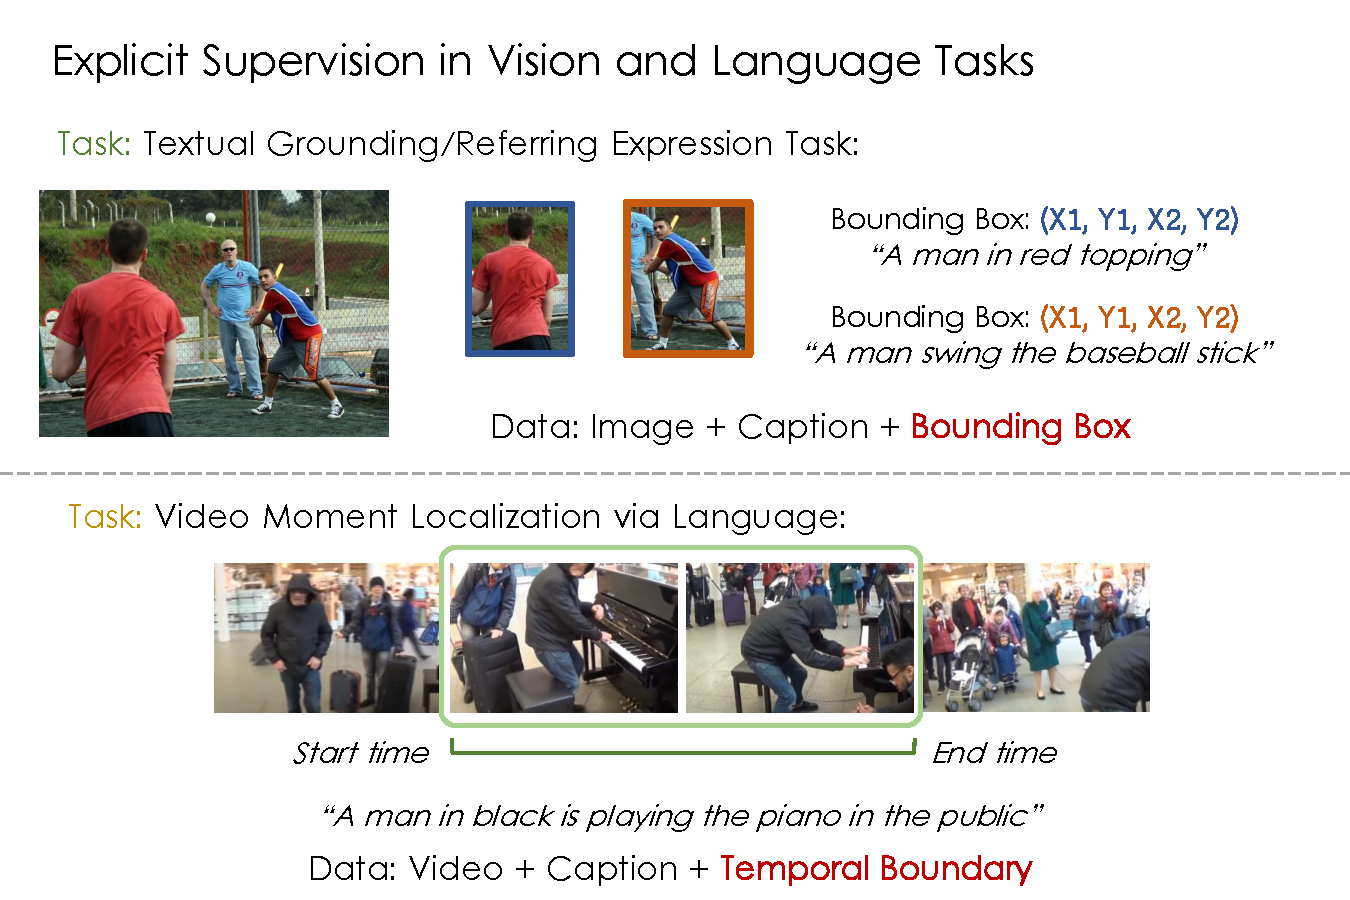
\includegraphics[width=.99\textwidth]{images/explicit_training.pdf}
\end{center}
\caption[Example of some VL tasks.]{VL tasks like textual grounding, referring expression and video moment localization via language unanimously require explicit annotations (\ie, bounding boxes of target objects or temporal boundaries for the moments) for learning of visual-textual correlation.
}
\label{fig:explicit_learning}
\end{figure}

Despite these, there exist several critical challenges that prevent us from pushing these advances to the real world.  One of the most difficult problems comes from the prohibitively expensive human labeling: previous powerful VL models are mostly domain-specific that rely heavily on a well-annotated VL dataset by humans, \eg, image captioning dataset like COCO~\citep{lin2014microsoft} collected  328K images, covering image-level object annotations and also captions explaining the content of images. Beyond that, the development of powerful VL systems like textual grounding models requires the awareness of spatial location per object (see Figure~\ref{fig:explicit_learning} for example). Compared with the countless images the system might encounter in the real world, annotating images at scale in COCO-style is hardly practical, nor financially effective. This spawns the challenge for the VL community: how to train a unified VL model that can be transferred to diverse domains via the implicit supervisions (\ie, large volume of weakly-annotated, or even un-labeled raw visual+textual data). Unlike the traditional vision model (object detection or recognition model), the VL model usually requires the understanding of correlations between visual concepts with rich semantics, while the traditional visual model only performs on a bunch of pre-defined and limited categories.


Another notable challenge arises when deploying the VL model on an edge device that usually has the limited computational power to be undertaken. It is impractical for real-world applications to exploit the power of prevailing VL models under a constrained training/inference budget due to their cumbersome sizes and huge computation cost. Building a lightweight VL model, meanwhile improving its performances is of great practical value but is less explored in the previous literature. In the furtherance of gaining a more real-world practical compact VL model, we study to exploit knowledge distillation techniques to improve the VL representation learning on compact models. 


Following the above-mentioned, I work on making contributions in the following aspects:

\begin{figure}
\begin{center}
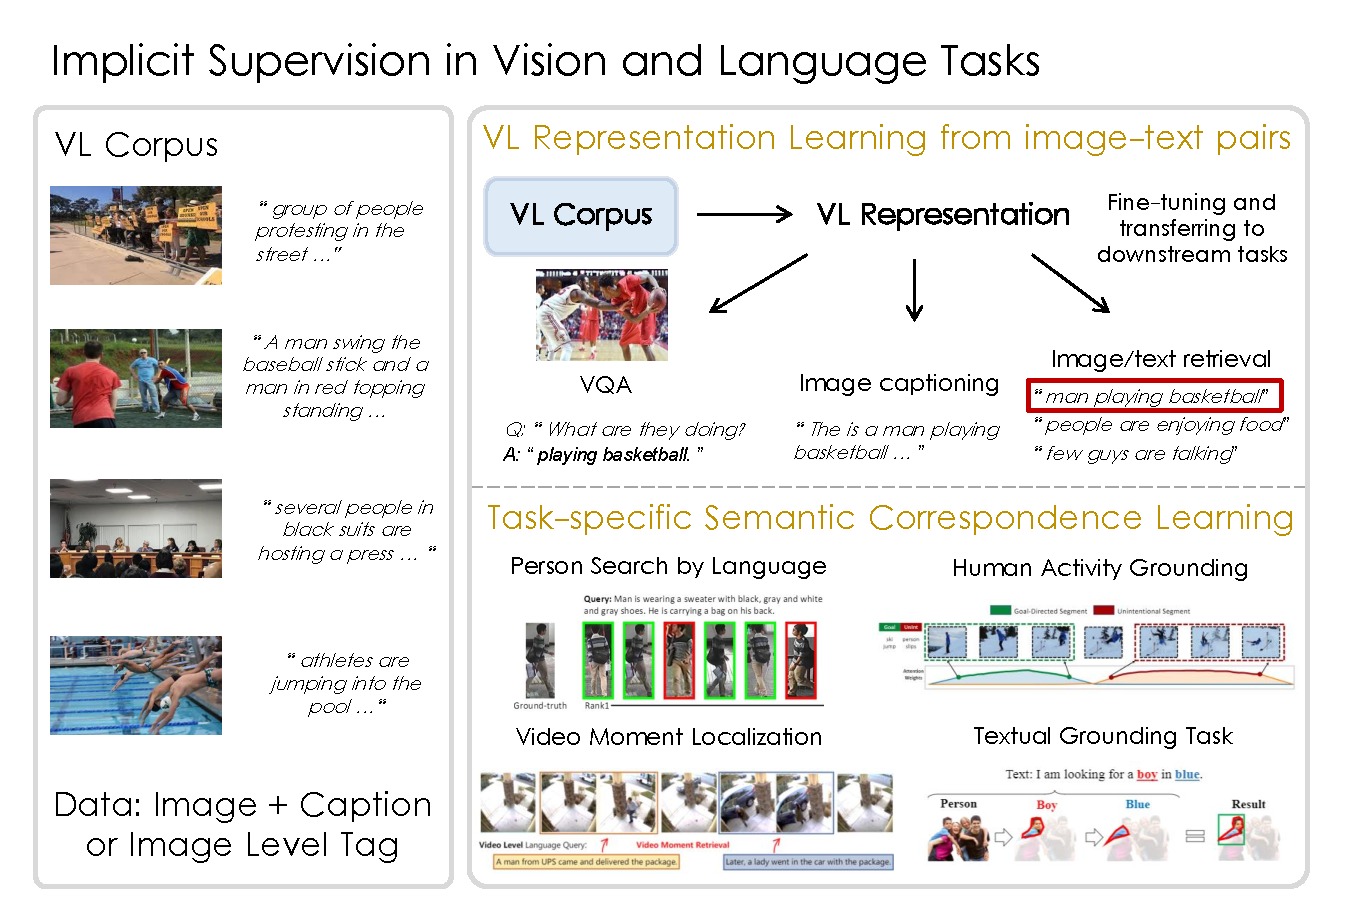
\includegraphics[width=.99\textwidth]{images/implicit_training.pdf}
\end{center}
\caption[VL Representation Learning \vs Downstream VL tasks.]{Unlike explicit VL supervisions, the training on implicit VL supervisions aims to learn either 1). task-agnostic and generic VL representations that can be transferred to other VL tasks, or 2). specific VL task (\eg, grounding, retrieval, etc). The former task focuses more on how to learn the VL representations from image-text pairs with better generalization and expressive semantics when there is no explicit training objective, while the latter requires a task-specific learning method (\eg, multi-instance learning).
}
\label{fig:implicit_learning}
\end{figure}

1. Learn the associations between visual concepts and semantics in a weak/un-supervised fashion. For example, when given an image, learn which specific region best corresponds to a textual query ``\textit{A man in red topping}'', when we have only an image-level general description like ``\textit{A man swing the base ball stick and a man in red topping standing in the playground ...}'', without knowing the exact region corresponds to specific visual concepts (a.k.a, weakly-supervised textual grounding in images/videos).

2. Learn ``omni''-VL representations that can be transferred to diverse VL tasks from image-text pairs via pre-training and fine-tune fashion. Now as the VL pre-training leverages only general image+text pairs without further spatial, or pixel-level annotations, it is challenging how to effectively mine the hidden visual-textual associations at scale for representation learning (as is shown in Figure~\ref{fig:implicit_learning}). Beyond that. I also work on leveraging task-agnostic knowledge distillation in assisting the representation learning on small and generic VL models. 

3. Build an efficient VL model. Much of the existing VL models focus on large models that suffer from high latency and large memory footprints at the time of inference, which limits their deployment to resource-constrained edge devices for real-world applications. I study how to train small and efficient VL models from the perspective of Knowledge Distillation for model compression. In the end, I explain the feasibility of developing the ``one-stage VL model'' which does not require the cumbersome object detector and thus brings obvious flexibility for both model training and inference. 

% Figure~\ref{fig:explicit_learning} gives an overview of the major aspects of this dissertation. 
This dissertation highlights a few selected research projects I worked on from the aforementioned perspective: 1). A textual grounding system that learns the semantic correspondence from weakly supervised learning~\citep{Fang_2019_CVPR,fang2019temporal}. 2). A novel self-supervised visual representation learning paradigm coupled with knowledge distillation~\citep{fang2020seed}. 3). A compact VL model that benefits from VL distillation, which can be transferred to a series of other generic downstream VL tasks~\citep{fang2021compressing}. Also an one-stage image captioning model that brings training flexibility and inference speed~\citep{fang2021injecting}. All of these efforts reflect my primary research in the intersection of computer vision and natural language processing that advances the V+L learning from implicit supervisions with increased efficiency.

\section{Preliminaries}
To give the readers a more comprehensive background introduction about the Vision and Language and some relevant techniques this dissertation mentions later, I will briefly review several Vision Language tasks, together with their formulation under the weakly-supervised learning schema. These weakly-supervised VL tasks are less data-dependent than they attempt to learn the cross-modal correspondence without explicit supervision. Nevertheless, they are inevitably limited to only specific VL tasks that need manual design. To circumvent these, a broader series of works alter to introduce the generic representation learning from a large VL corpus that their ``omni''-representations are transferable to different downstream tasks and are entirely task-agnostic during the pre-training phase.

\subsection{Glance of Prevailing VL Tasks}


\begin{figure}
\begin{center}
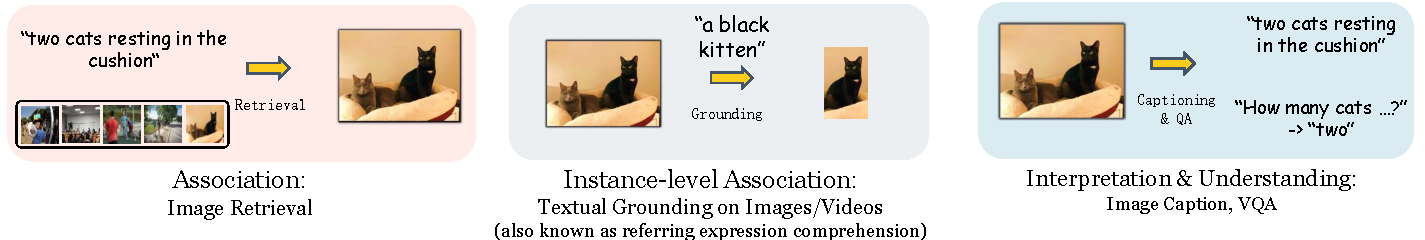
\includegraphics[width=.99\textwidth]{images/VL-tasks.pdf}
\end{center}
\caption[Prevailing VL Tasks.]{Glance of some representative VL tasks from different perspectives. The image content retrieval task builds upon the association relationship across the Vision and Language modalities. Proceeding from that, this association extends to the instance-level that one can retrieve either a region of the image covering a specific object or a short video moment containing an event in untrimmed video. High-level VL tasks involve more interpretation and understanding: for instance, generating a textual description from the observation, or answering the question based on the visual observation.}
\label{fig:VLtasks}
\end{figure}

\noindent{\bf Association Learning across Vision and Language} is core and tie of a wide range of tasks across vision and language domains, \emph{e.g.}, textual grounding~\citep{plummer2015flickr30k}, referring expression comprehension~\citep{nagaraja2016modeling} or object retrieval using language~\citep{hu2016natural}. In particular, given an image $\mathbf{I}$, {T}extual {G}rounding model selects a proposal $\mathbf{c}$ given a textual query $\mathbf{T}$ from a set of coordinates $\mathbf{C} = \{\mathbf{c_1 \dots c_N}\}$ (see example in Figure~\ref{fig:VLtasks}):
\begin{equation}
    \mathbf{c} = \text{Textual-Grounder}{\big(}\mathbf{I}, \mathbf{T},\mathbf{C}{\big)},
\end{equation}
where $N$ denotes the number of candidate proposals generated by some generic proposal network. To obtain a strong textual grounding model, one might need to collect massive \texttt{<image-text-proposal>} triplets to sufficiently train such a model. 
Such association learning also extends to the video domains ({V}ideo {L}ocalization Task) where the textual description is utilized as the query to anchor a clip from a long untrimmed video:
\begin{equation}
    \mathbf{c} = \text{Moment-Localizer}{\big(}\mathbf{V}, \mathbf{T}, \mathbf{C}{\big)},
\end{equation}
where now the proposal $\mathbf{c}$ is selected as the temporal boundary of a video moment with starting time $t_s$ and ending time $t_e$ of the video $\mathbf{V}$.

Recent works shed light on the importance of leveraging the image-level annotations (as weak supervision)~\citep{fang2018modularizedtextual,fang2018weakly} or unsupervised method~\citep{yeh2018unsupervised} to learn the association across language descriptions and objects. Proceeding from this, there arise works on using uncurated captions to learn temporal associations across video segments and texts~\citep{miech2019end,sun2019videobert}. Notably, these works all highlight the importance of constructing contrastive pairs in exploiting the weak annotations. We will discuss more about the contrastive learning at later section. 

\noindent{\bf Visual Interpretation via Language} tasks laid more emphasis on the high-level understanding aspects. Typical interpretation tasks include \emph{Visual Captioning} and \emph{Visual Question Answering} Tasks (an example is shown in Figure~\ref{fig:VLtasks}). Visual captioning is perhaps the first step towards understanding images/videos and describing their content in natural language.
Recent advances in visual captioning have been able to generate captions that describe humans and objects and their interactions in the video.
They seek to generate paragraphs or multi-sentence captions about the content of images or videos.
It is important to note that visual captioning systems have a major limitation in that they can only generate factual descriptions about observable objects or events in the video yet without full \emph{understanding} the content. For detailed visual understanding, we would like to go beyond observable visual entities and use background knowledge and contextualization to reason about the observation and answer the questions. Most existing VQA benchmarks only predict answers from a pre-constructed \& limited answer sets, largely limits the practical scopes of the systems. Few recent works propose the open-domain VQA task~\citep{chang2021webqa} that generates the answers directly, or the VQA tasks need external knowledge~\citep{wang2017fvqa,zellers2019vcr,marino2019ok,garcia2020knowit,7298682}


\subsection{Implicit Supervisions for VL Tasks}
\noindent{\bf Weakly Supervised Learning} receives increasing attention~\citep{deselaers2010localizing,pandey2011scene, cinbis2017weakly,mahajan2018exploring,pathak2015constrained,pinheiro2015image,xu2014tell}.
It focuses on learning granular detectors given only coarse annotations.
This is of practical significance as granular annotations (\eg, bounding boxes and pixel-level labels) are much more expensive to obtain compared to coarse image-level annotations.
Recent studies show that weakly supervised methods can even outperform the strongly supervised method for image classification~\citep{mahajan2018exploring,ge2019weakly},
and is even widen to a wide range of vision tasks, including object detection~\citep{bilen2014weakly,shen2018generative,bilen2016weakly}, semantic segmentation~\citep{kervadec2019constrained,pathak2015constrained,wei2016stc} and etc.
In video analysis domain, the weakly-supervised action localization is frequently studied and can be thought of a specific example of learning with the video-level labels~\citep{sun2015temporal,shou2018autoloc,nguyen2018weakly,paul2018w}.
This problem derives from the fully-supervised counterpart methods which exploits fine annotations at frame level
for localizing the actions~\citep{buch2017sst,kalogeiton2017action,weinzaepfel2015learning,shou2017cdc,tran2012max,shou2016temporal}.
Recent weakly-supervised methods extensively adopt either the video-level classification framework~\citep{singh2017hide,shou2018autoloc,sikka2014classification,dwibedi2019temporal} or with the attentional mechanism 
that generates bottom-up sparse weights used for localizing action categories temporally~\citep{nguyen2018weakly}. Beyond that, few works~\citep{wang2017untrimmednets,paul2018w} propose to utilize the multi-instance learning loss to address this challenge,~\citep{paul2018w} also suggests exploiting the co-activity across videos in the metric learning, which largely improves the action localization task even when temporal annotations are not available. The most recent work~\citep{nguyen2019weakly} improves over these methods with a background modeling module that explicitly extracts the foreground and background appearances.  This dissertation focus more on extending this weakly supervised learning signals to VL tasks.\footnote{Implicit supervisions in this dissertation refer to both weakly-supervised learning and self-supervised learning.}

% Unlike current work,
% we perform weakly-supervised learning for textual grounding, including training for both entity grounding
% and textual-visual matching through a progressive modular procedure.

% Modular design is also receiving more attention recently, mainly for
% complex systems like visual-question-answering or image captioning~\citep{hu2017modeling, hu2018explainable,
% yu2018mattnet}.
% Such modular design is carried out by realizing some linguistic structures.
% In our work,
% we propose to decompose the query textual description into progressive levels,
% each of which is passed to a corresponding module,
% and then produce the final grounding result by progressively merging the intermediate results.
% In this way,
% our system enjoys high interpretability and resilience to counterfactual inputs.

% Few works also shed light upon the importance of contrastive learning for weak supervision.


\noindent{\bf Weakly-Supervised Image/Video Grounding by Language} 
We are concerned with the model's dependency on the complicated data annotations for textual grounding task. For this reason, it is important to study how to build 

Temporal Grounding and Moments Retrieval are two instantiations of learning
temporal-textual association.
In these tasks, most recent methods adopt fully-supervised training over 
fine annotations on the frame-textual associations.
For example, Gao \emph{et al.} augment the Charades 
dataset~\citep{sigurdsson2016hollywood} by generating complex language queries with temporal boundary annotations for language moment retrieval~\citep{gao2017tall}; 
Anne Hendricks \emph{et al.} also collect a new dataset for training to localize video moments over a given descriptive sentence~\citep{anne2017localizing}. 
Other follow-up methods~\citep{hendricks2018localizing,liu2018attentive,chen2018temporally,wang2018bidirectional,xu2019joint,gavrilyuk2018actor} also
fully-supervised train for temporal grounding using these datasets,
suffering from the limitation on their generalizability due to  
the combinatorial nature of complex natural language sentences (\textit{e.g.}, 
synonymous words, grammatical tense 
and sentence structures)~\citep{hendricks2018localizing,gao2017tall}. 
advances the aforementioned to an even challenging task, as now the only available supervision is video-level natural language descriptions in an open format, which come with a huge amount of unnecessary noises.
In particular, Mithun \emph{et al.}~\citep{Mithun_2019_CVPR} for the first time attempted to 
solve the temporal grounding problem by weakly supervising learning 
with only the video-level textual queries~\citep{Mithun_2019_CVPR}. 
In~\citep{chen2020look}, the author proposed to utilize the temporal proposal and textual description alignment learning using the sliding window fashion and tackle the grounding problem in a coarse-to-fine manner. Similarly, a very recent work by~\citep{lin2019weakly} also focuses on the design of a better proposal generation module, that aggregates the contextual visual cues to generate and score the proposed candidates for grounding. We summarize that current efforts in weakly supervised language grounding are either centered on better proposal generation~\citep{chen2020look,lin2019weakly} or a better cross-modal association model by constructing contrastive samples across video and languages~\citep{Mithun_2019_CVPR,gao2019wslln}. Our WSRA (introduced in later Chapter) places emphasis on the latter, but nevertheless further distinguishes the above with a more comprehensive cross-modal association learning objectiveness and a novel sampling and weighting strategy in our metric learning step.

\subsection{VL Representation Learning from Weak Annotations}

Following the prominent progress in the transformer-based (introduced in later section)~\citep{vaswani2017attention} pre-training in natural language~\citep{devlin2018bert,radford2018improving,lagler2013gpt2,brown2020language,clark2020electra,raffel2019exploring}, Vision Language pre-training models, either for image+text~\citep{lu2019vilbert,tan2019lxmert,chen2019uniter,li2020oscar,hu2020vivo,zhang2021vinvl,li2020closer,gan2020large,li2020hero,lu202012} or for video+text~\citep{sun2019videobert,li2020hero,miech2020end,zhu2020actbert,lei2021less}, have achieved great success on a number of downstream V+L tasks. 

\subsection{Self-supervised Learning and Contrastive Learning}
Another important implicit supervision is the self-supervised learning technique. 
Among the recent works in \textbf{Self-supervised Learning (SSL)}, contrastive based approaches show prominent results on downstream tasks. Majority of the techniques along this direction are stemming from noise-contrastive estimation~\citep{gutmann2010noise} where the latent distribution is estimated by contrasting with randomly or artificially generated noises. 
~\citep{oord2018representation} first proposed Info-NCE to learn image representations by predicting the future using an auto-regressive model for unsupervised learning. Follow-up works include improving the efficiency~\citep{henaff2019data}, and using multi-view as positive samples~\citep{tian2019contrastive1}. As these approaches can only have the access to limited negative instances,~\citep{wu2018unsupervised} designed a memory-bank to store the previously seen random representations as negative samples, and treat each of them as independent categories (instance discrimination). However, this approach also comes with a deficiency that the previously stored vectors are inconsistent with the recently computed representations during the earlier stage of pre-training. ~\citep{chen2020simple} mitigate this issue by sampling negative samples from a large batch. Concurrently,~\citep{he2020momentum} improve the memory-bank based method and propose to use the momentum updated encoder for the remission of representation inconsistency. Other techniques include~\citep{misra2020self} that combines the pretext-invariant objective loss with contrastive learning, and ~\citep{wang2020understanding} that decomposes contrastive loss into alignment and uniformity objectiveness.


\subsection{Knowledge Distillation}
Knowledge Distillation has been applied to model compression task across different domains with its main goal being to transfer the ``\textit{knowledge}'' $f(x_i)$ of sample ($x_i, y_i$) from a strong Teacher network ($T$) to the Student network ($S$) by minimizing the divergence between them:
\begin{equation}
\mathcal{L} = \frac{1}{N}\sum_{i=1}^{N}\bigg(\mathcal{L}_\text{S}(x_i, y_i) + \mathcal{L}_\text{KD}\Big(f^S(x_i), f^T(x_i)\Big)\bigg),
\end{equation}
where $\mathcal{L}_\text{S}(\cdot)$ refers to the original supervision signal(s) on the Student. In practice, this term can possibly be replaced by the exclusive use of $L_\text{KD}$. Depending on the type of knowledge transferred, $\mathcal{L}_\text{KD}$ can derive from soft cross-entropy, mean squared error (MSE) function or \textit{KL}-divergence.
For example,~\citep{hinton2015distilling,bucilua2006model} transfer the learned knowledge by mimicking the mass function of the output probability across classes, or by minimizing the divergence of intermediate features~\citep{yim2017gift,koratana2019lit,huang2017like,yalniz2019billion,xie2020self}.
Works in ~\citep{ahn2019variational,yim2017gift,koratana2019lit,huang2017like} have utilized different learning objectives including consistency on feature maps, consistency on probability mass function, and maximizing the mutual information. CRD~\citep{tian2019contrastive}, which is derived from CMC~\citep{tian2019contrastive1}, optimizes the student network by a similar objective to~\citep{oord2018representation} using a derived lower bound on mutual information. 
~\citep{tian2019contrastive,tian2019contrastive,fang2021seed} propose contrastive distillation for visual representation learning.  In addition, remarkable advances have been made in knowledge distillation for language model compression (\ie, BERT~\citep{devlin2018bert}), and these works show that mimicking the distribution of self-attention and intermediate representations of transformer blocks increases performances~\citep{sanh2019distilbert,jiao2019tinybert,sun2020mobilebert,xu2020bert} for downstream tasks.
In particular, in the transformer-based language model distillation, DistillBERT~\citep{sanh2019distilbert} proposes to train the small BERT by mimicking the Teacher's output probability of masked language prediction and the embedding features.  TinyBERT~\citep{jiao2019tinybert} and MobileBERT~\citep{sun2020mobilebert} leverage the layer-wise attention distributions for distillation with MSE function.~\citep{wang2020minilm} suggests distilling on the last transformer layer and bringing extra flexibility for training.~\citep{sun2020contrastive,chen2020wasserstein} also use the contrastive distillation in transformer-based language model compression.~\citep{fang2021seed,sun2020contrastive} propose using a sample queue to store history embeddings and show that contrasting with more negative samples is beneficial for knowledge distillation. 

\subsection{Architecture of VL Model}
Most existing VL models are designed in a two-step fashion: a pre-trained object detector is used to encode the image as
set of regional features (as offline visual tokens) followed by pre-training on a large scale visual-linguistic corpus using tasks like masked language modeling, image-text matching or masked region modeling losses. In particular, Zhang \etal~\citep{zhang2021vinvl} demonstrate the significant role of visual features in VL pre-training and looks for more effective visual representations from a larger object detector. Li~\etal~\citep{li2020oscar} shows that a larger transformer VL model can learn better from larger VL corpus. However, the marginal costs are greater than the marginal benefits. 
Recently, Wang \etal~\citep{wang2020minivlm} propose a small VL model called MiniVLM that uses a lightweight visual feature extractor and smaller transformer to reduce the model size by 73\% and maintain good accuracy on VL tasks. 
Nevertheless, the cost of pre-training on MiniVLM is associated with sub-optimal efficiency: it requires a large amount of training data (14M) to learn a good representation. Thus, it is worth exploring a more efficient way to train small VL models. 
There are other lines of VL pre-training works in which grid features~\citep{huang2020pixel,jiang2020defense} is extracted from the convolutional layers without the proposal computation.~\citep{ramesh2021zero,radford2021learning,desai2020virtex} learn visual representation from scratch using Convolutional Neural Network as image encoder with a transformer for VL pre-training on a large amount of image-text pairs.  The notion of VL distillation is not limited to just the two-stage VL models, it can potentially benefit other types of transformer-based VL models as well. 



\begin{figure}[t]
\centering
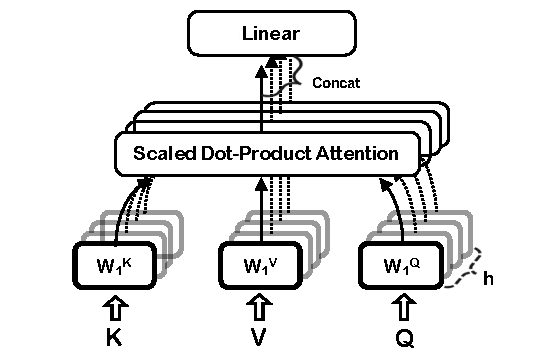
\includegraphics[width=.45\textwidth]{./images/attention.pdf}
\caption{ Illustration of Multi-Head Attention block. Each block consists of $L$ attention layers. 
}
\label{fig:multiattention}
\end{figure} 

\subsubsection{Transformer Model}
A Transformer Model is composed of a stack of identical transformer blocks, whose main component is a self-attention architecture.
It takes as input the summation of word embedding and the positional encoding offset by 1 position through a masked multi-head attention block, which prevents future words from being seen by the block. 

The transformer block consists of several consecutive linear transformations.
Let $\mathcal{H}_{\textsc{M-Att}}$ denotes the multi-head attention block, $\mathcal{H}_{\textsc{Norm}}$ be the normalization layer and $\mathcal{H}_{\textsc{FFN}}$ be the feed forward layer.
Let K, V, and Q denote the key, value, and query respectively, which are inputs to the attention block.
The transformer block can be summarized as follows:
\begin{equation}
\begin{split}
\tilde{o_1}^\ell&=\mathcal{H}_{\textsc{M-Att}}(\textrm{K}, \textrm{V}, \textrm{Q}) \\
\tilde{o_2}^\ell &= \mathcal{H}_{\textsc{Norm}}(\tilde{o_1}^\ell + \tilde{\mathbf{o}}^{\ell-1})   \\
\tilde{o_3}^\ell &= \mathcal{H}_{\textsc{FFN}}(\tilde{o_2}^\ell)   \\
\tilde{o}^{\ell}&= \mathcal{H}_{\textsc{Norm}}(\tilde{o_3}^\ell \tilde{o_2}^\ell),
\end{split}
\end{equation}
In the context of the transformer blocks used in our work, the video encoding acts as the key, the concatenation of video/caption encoding is the value, and the output from the previous transformer block acts as the query.


\subsubsection{Multi-head Attention Block}
\label{sec:att_block}
In the masked multi-head attention block, the transformer block is used with K, V, and Q being identical vectors of the input embedding.
An example of a multi-head attention block is shown in Figure~\ref{fig:multiattention}.
The motivation of the design originates from the self-attention mechanism that aims to solve the problem of long-term dependencies because of which the propagated gradients tend to vanish or explode. 
    Instead of handling sequences word by word, the self-attention block learns the attention weight between every word and produces a representation with a global view of the input.
A self-attention block with $L$ heads is formulated as: 
\begin{equation}
\mathcal{H}_{\textsc{M-Att}}(\textsc{K}, \textsc{V}, \textsc{Q}) = \mathcal{H}_{\textsc{FFN}}([{g_1}, {g_2}, ..., {g_L}]).
\end{equation}
$g_i$ for every head-index $i$ is computed by a scaled dot-product attention operation as:

\begin{equation}
{g_i} = \textsc{Softmax}\xbigg(\frac{\textsc{w}^\textsc{q}_i \textsc{Q}\cdot \textsc{w}^\textsc{k}_i \textsc{K}^\prime}{\sqrt{d_k}}\bigg)\textsc{w}^\textsc{v}_i \textsc{V}, \forall i \in \{1, \dots, L \},
\end{equation}
where $d_k$ is the dimension of keys, and $\textsc{w}_i$ are the learnable parameters of the linear transformation.

% \section{Related Literature}


In what follows, we will introduce our progress towards each perspective as stated above. In Chapter 2, we summarize our effort to build a VL grounding model from weak supervisions, achieving satisfactory grounding results compared with explicit supervised models. Furthermore, we also investigate the effort of extending the weakly-supervised grounding to videos. In Chapter 3, we then introduce a novel self-supervised visual representation learning algorithm that is facilitated by knowledge distillation technique which achieves major performance gain. We extend this contrastive learning-based distillation algorithm to the VL representation learning on a small VL architecture. Chapter 4 presents a one-stage VL model that is object detector-free and can be end-to-end optimized dubbed ViTCAP, experiment shows that our ViTCAP reaches state-of-the-art image captioning performances amongst all existing one-stage VL models. We finally summarize our work and point some future research directions in the end.                  

% \include{seed}
% 

\section{VL Representation Learning via Knowledge Distillation on Compact Architectures}



\begin{figure}[h]
    \centering
    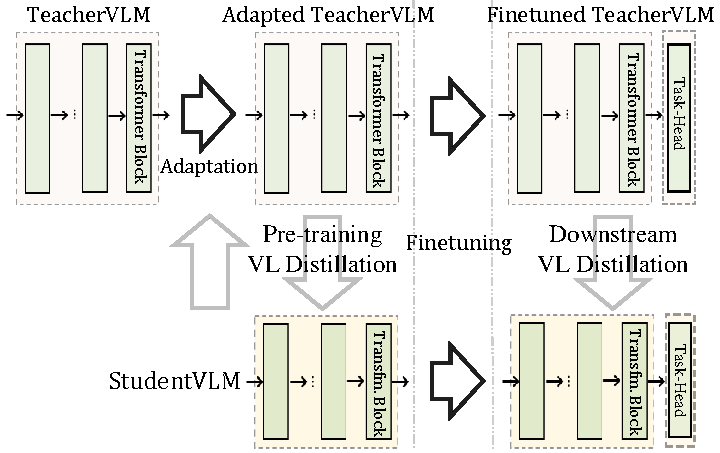
\includegraphics[width=.95\textwidth]{images/distillvlm_abstract.pdf} 
    \caption[Overview of our proposed VL distillation schema. ]{ Overview of our proposed VL distillation schema. 
    The VL model typically contains a region feature extraction module and a multi-modal transformer module. To have an aligned input, we adapt the Teacher VL model based on the region proposals from Student's region feature extractor. The VL distillation is then performed in both the pre-training stage and the fine-tuning stage.
    }
    \label{fig:abstract}
\end{figure}


%%%%%%%%% BODY TEXT
As previously mentioned, there have been exciting progress in visual linguistic~(VL) pre-training to learn omni-representation models~\cite{lu2019vilbert,su2019vl,chen2019uniter,tan2019lxmert,zhou2020unified,li2020oscar} which could benefit a number of downstream tasks (\ie, image captioning, VQA, image retrieval, etc.). The success can largely be attributed to the self-attention-based~\cite{vaswani2017attention} transformer architecture, \eg, BERT~\cite{devlin2018bert}, which is effective in learning from image-text pairs at scale. So far, much of the work has focused on large models that suffer from high latency and large memory footprints at the time of inference, which limits their deployment to resource constrained edge devices for real-world applications. 


As one of the effective techniques to compress large models, 
knowledge distillation (KD)~\cite{hinton2015distilling, bucilua2006model} was proposed  by injecting the knowledge from a strong Teacher model into a smaller Student model without losing too much generalization power. 
Typically, the knowledge is transferred though
mimicking the output logit~\cite{hinton2015distilling,sanh2019distilbert,fang2021seed}, reducing the divergence of feature maps~\cite{zagoruyko2016paying,NST2017,yim2017gift}, or learning the intermediate layer representations~\cite{koratana2019lit,ahn2019variational}, \etc. 

In recent years, KD has been proven effective in compressing language models. For instance, Kim \etal~\cite{kimrush2016sequence} adopt KD for sequential model compression. In the transformer based language model, DistillBERT~\cite{sanh2019distilbert} reduces the size of the BERT-base model by 40\% using a cosine embedding loss on the basis of hidden embedding in the transformer block, and a soft-target probability loss. TinyBERT~\cite{jiaoetal2020tinybert}, MobileBERT~\cite{sun2020mobilebert} and MiniLM~\cite{wang2020minilm} further highlight the importance of minimizing the self-attention distributions across Teacher and Student networks. In particular,~\cite{clark2019does} visually shows that attention maps in BERT capture substantial linguistic knowledge and syntactic relations that provide critical information during the distillation~\cite{jiaoetal2020tinybert}.

Heretofore, these advances have not been carried over to VL model compression.
We identify the major challenges that prevent us from applying these techniques directly to VL distillation:
Most existing VLP works~\cite{zhou2020unified,li2020oscar} use pre-trained object detector (\eg, Faster-RCNN~\cite{ren2015faster}) to extract regional features as visual tokens then feed them into the multi-modal transformer network for VL pre-training.
A smaller VL model usually uses a lightweight detector for faster inference (\eg, EfficientNet~\cite{tan2019efficientnet} based detector is adopted in~\cite{wang2020minivlm} as visual feature extractor) that may be different from Teacher's detector. The object proposals from the two different detectors are usually very different, and there is no easy way to obtain the semantic correspondence between the two sets of object proposals. It is therefore unable to align the attention distributions or hidden embeddings between Student and Teacher.

To address the aforementioned challenges, we propose a set of strategies to enable distillation of VL models. First, instead of using object proposals from two different detectors, we use the same set of object proposals, obtained from Student's lightweight detector for the visual token extraction of both Teacher and Student (as shown in Figure~\ref{fig:arch}). This ensures the semantic correspondence between the Teacher and Student's visual tokens. Second, we use a loss term to have the Student to mimic the Teacher's self-attention distribution at the last transformer layer. Third, We further distill the knowledge from the outputs of the transformer layers (\ie, the hidden embeddings). We find that simply learning from the layer-wise Teacher embedding does not provide adequate supervision for the  distillation. Hence, we use a noise contrastive loss to align the token embeddings by contrasting them with randomly sampled negative embeddings that are held in a sample queue. 
Figure~\ref{fig:abstract} gives an overview of our proposed VL distillation schema, where VL distillation is applied for both the pre-training and fine-tuning stages.
In order to examine the effectiveness of our VL distillation, we 
choose the same compact transformer architecture used in~\cite{wang2020minilm,wang2020minivlm}, and the lightweight object detector as in~\cite{wang2020minivlm}, but leverages knowledge distillation techniques to facilitate the training of the small VL model (dubbed as \distillvlm). 
We show that our \distillvlm achieves a comparable performance to a large VL model, and clearly outperforms its non-distilled counterpart~\cite{wang2020minivlm}.

To summarize our contributions:  \\ [-2.5ex]
\begin{itemize}[noitemsep,nosep]
    \item For the first time, we propose VL distillation, a technique that leverages knowledge distillation to facilitate training of smaller VL models. \\ [-1.7ex]
    \item Compared to non-distilled VL model pre-training, VL distillation offers a significant boosting in performance for VL tasks such as image captioning and visual question answering: DistillV{\small L}M achieves 120.8 in  CIDEr score on COCO captioning~\cite{lin2014microsoft} and 69.8 in accuracy on VQA~\cite{balanced_vqa_v2} tasks, which are $5.1$ more or $0.8$ higher than the VL pre-training baselines.\\ [-1.7ex]
    \item We provide extensive ablations of \distillvlm, and systematically analyze the effect of various KD strategies.
    This provides insights for future research on VL model distillation.
\end{itemize}



\begin{figure*}[th!]
    \centering
    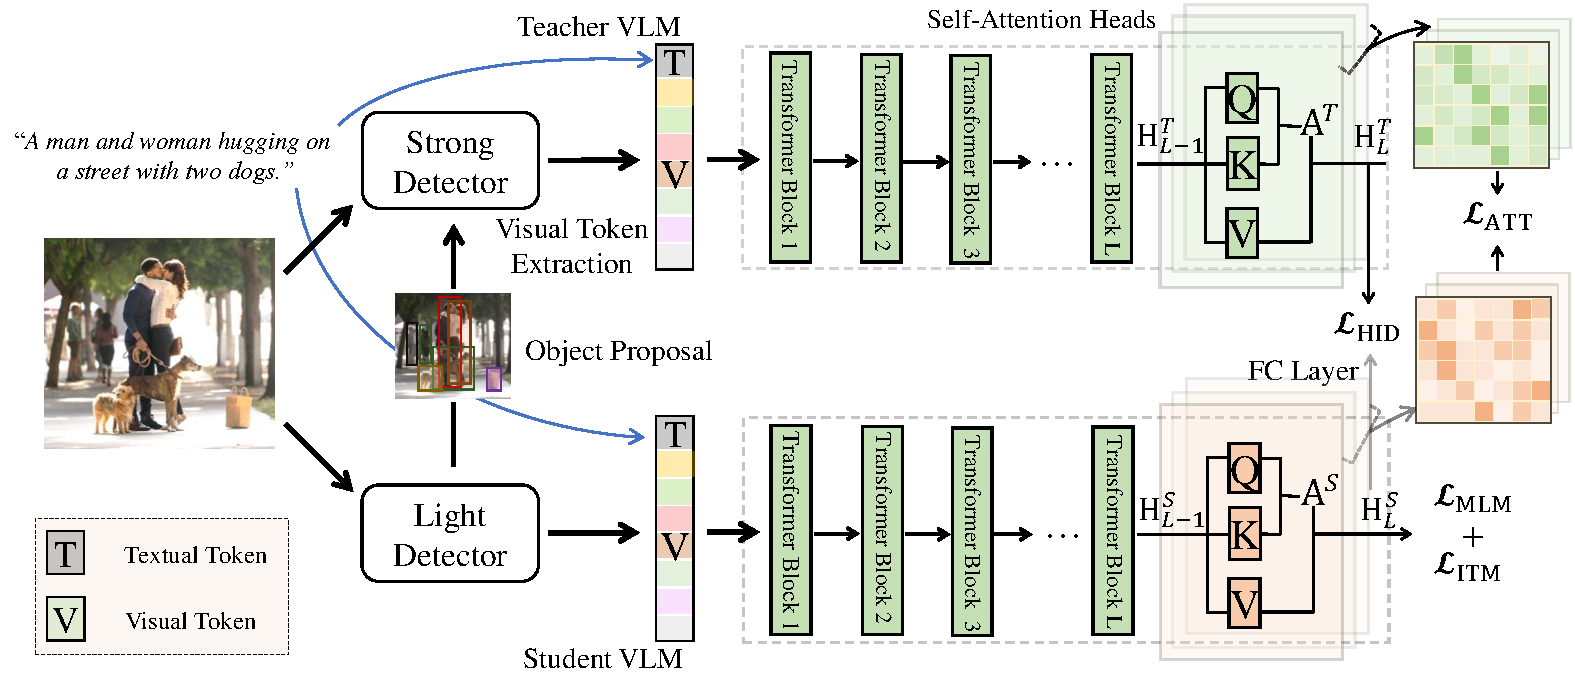
\includegraphics[width=.98\textwidth]{images/distillvlm_architecture.pdf} 
    % \vspace{1mm}
    \caption[Illustration of our proposed DistillV{\footnotesize L}M architecture.]{ 
    {
    Illustration of our proposed DistillV{\footnotesize L}M architecture. The lightweight detector extracts the region features, and the region proposals are injected into the strong detector so that the region features are aligned between Teacher and Student. The Teacher transformer network is adapted with the new input before distillation. The Student VLM is distilled based on the hidden embedding matching and attention distribution alignment. 
    }
    }
    \label{fig:arch}
\end{figure*}

\subsection{Visual-linguistic Knowledge Distillation}
Compared to knowledge distillation in language models, VL knowledge distillation requires knowledge transferring from Teacher to Student in both modalities.
We present {DistillV{\small L}M} for the task of visual-linguistic distillation (the overall architecture is illustrated in Figure~\ref{fig:arch}), together with the detailed strategies for our model training. 

\subsubsection{Visual Token Alignment}
VL pre-training methods such as  OSCAR~\cite{li2020oscar} take as input an image-text pair in the format of Word-Tag-Image triple ($\boldsymbol{w}$, $\boldsymbol{q}$, $\boldsymbol{v}$), where $\boldsymbol{w}$ and $\boldsymbol{q}$ denote the sequence of caption embedding and the word embedding of detected object tags (in texts). 
To obtain the visual tokens $\boldsymbol{v}$ and object tags, a set of image regional vectors are extracted from an object detector. A Faster R-CNN~\cite{NIPS2015_14bfa6bb} detector pre-trained on Visual Genome~\cite{krishna2017visual} is used to extract the visual feature vector of each region, which is concatenated with its regional position coordinates to form a positional-sensitive region feature vector. This vector is then fed into a linear projection to ensure that the final vector $\boldsymbol{v}$ has the same dimension as the caption/tag embedding. The VL pre-training can be seen as a semantic alignment process between the image regions and the textual units. It is worth mentioning that, the top regions to be extracted from the image
is dependent on their associated confidence score output by the detector~\cite{wang2020minivlm}, which leads to some over-sampled and noisy visual tokens. Typically, the order of visual tokens is specified in descending order using the confidence score.
As an alternative to Faster-RCNN, MiniVLM~\cite{wang2020minivlm} uses a lightweight detector (\ie, TEE) in which the backbone is replaced with EfficientNet~\cite{tan2019efficientnet} and a BiFPN~\cite{tan2020efficientdet} module is added to generate multi-scale features. These strategies obviously accelerate inference process, but inevitably also lead to different visual tokens between the Teacher and Student networks during distillation. For this reason, the direct application of the distillation loss to attention matrices or hidden representations leads to an invalid transfer of knowledge. Hence, we extract and align the Teacher/Student's visual tokens by using the same set of detected bounding boxes recognized by the lightweight detector, and keep the same token orders based on their confidence scores (as in Figure~\ref{fig:arch}). Both the Teacher and Student VLM use the same object tags from the lightweight detector during the distillation. Having the Teacher use the visual tokens extracted by proposals from the lightweight detector may result in small performance drop. In practice, we address this issue by fine-tuning/re-training the Teacher VLM using the new visual tokens (Teacher adaptation).


\subsubsection{Attention Distribution Distillation}
One critical component of the transformer block is the multi-head self-attention module~\cite{vaswani2017attention}.  which enables contextualized information to be captured from an input sequence. A multi-head attention module outputs a set of attended values:
\begin{equation}
    \texttt{Attention(}\mathbf{Q}, \mathbf{K}, \mathbf{V}\text{)}=\texttt{softmax(}\frac{\mathbf{Q}\cdot \mathbf{K}}{\sqrt{d_k}}\text{)}\cdot \mathbf{V},
\end{equation}
where $\mathbf{Q}$, $\mathbf{K}$, and $\mathbf{V}$ denote query, key and value that are retrieved after three independent linear transformations on the hidden embedding $\mathbf{H}_i$ from $i$-th transformer block, and $d_k$ is the dimension of key as a scaling factor. The dot-product between key and query after the softmax normalization is the attention matrix:
\begin{equation}
    \mathbf{A}=\texttt{softmax(}{\mathbf{Q}\cdot \mathbf{K}}/{\sqrt{d_k}}\text{)}.
\end{equation}
Each transformer block consists of a set of consecutive linear transformations, which include one multi-head attention module, a two-layer feed forward network, followed by a normalization layer, and finally a residual connection.


Previous attempts in language model distillation~\cite{jiao2019tinybert, sun2020mobilebert} have demonstrated the importance of transferring self-attention matrices, that are believed to contain latent linguistic information, \eg, syntactic and co-reference relation of input tokens~\cite{clark2019does,jawahar2019does}. 
~\cite{wang2020minilm} shows that using just the last transformer block's attention map yields equivalent results, allowing the Teacher and Student to have a different number of layers. In the case of the VL pre-training task, Cao \etal~\cite{cao2020behind} show that certain attention matrices of the pre-trained VL models contain extensive intra-modal and cross-modal co-reference relations.
These visual-linguistic knowledge is implicitly encoded, but shows a very promising potential for VL distillation.
We formulate the distillation loss of the attention distribution by minimizing the divergence between the self-attention matrices of the last layer of the Teacher and the Student:
\begin{equation}
    \mathcal{L}_\text{ATT} = \frac{1}{T\!\cdot\!H}\sum_{i=1}^{T}\sum_{j=1}^{H} \texttt{MSE}(\mathbf{A}^S_{i, j}, \mathbf{A}^T_{i, j}),
\end{equation}
where $T$, $H$ denote the number of tokens and attention heads in a transformer. $\mathbf{A}_{i, j}$ is the normalized attention for $i$-th token at $j$-th head. 
We further study the effects of the distillation over the attention distribution in ablations.

\subsubsection{Hidden Representation Distillation}
Similar to previous works~\cite{jiao2019tinybert,sun2020mobilebert}, we also use the hidden representations for the Teacher and Student alignment during distillation. In particular, previous efforts formulate the task as minimizing the divergence of the hidden embedding ($\mathbf{H}\in\mathbb{R}^{T\times d}$) of every Transformer block, whose objective is as follows:
\begin{equation}
    \mathcal{L}_\text{HID-MSE} = \frac{1}{T\!\cdot\!L}\sum_{i=1}^{T}\sum_{j=1}^{L} \texttt{MSE}(\mathbf{H}^S_{i, j}\mathbf{W}_{h}, \mathbf{H}^T_{i, j}),
\end{equation}
and $L$ stands for the number of transformer blocks. $\mathbf{W}_{h}$ is a learnable linear transformation that maps the Student hidden embedding into the identical dimension of Teacher embedding. However, there are limitations for such layer-to-layer alignment method. For example, TinyBERT must employ a uniform-function mapping to selectively choose a subset of the layers for learning, and MobileBERT requires the Teacher and Student to have identical number of layers. Since visual tokens are noisy during the VL distillation, this also leads to an increased difficulty in alignment. Sun \etal~\cite{sun2020contrastive} propose CoDIR, which takes advantage of the noise contrastive estimation (NCE) loss to align the Teacher \& Student's hidden representations by contrasting the target instance ($\mathbf{h}^S$) with more random instances as negative samples and aligning with its positive sample ($\mathbf{h}^T$), $\mathbf{h}\in\mathbb{R}^{d_T}$. Following~\cite{he2020momentum,fang2021seed,sun2020contrastive}, we employ a pre-defined instance queue $[\mathbf{h}_0^T, \mathbf{h}_1^T \cdots \mathbf{h}_K^T]$ to store $K$ random sampled embeddings and one positive embedding from the Teacher network. And the objective of NCE is as:
\begin{equation}
\mathcal{L}_\text{HID} = -\text{log} \frac{\text{exp}(\mathbf{h}^S_i\cdot\mathbf{h}^T_i/\tau)}{\sum_{j=0}^K\text{exp}(\mathbf{h}^S_i\cdot\mathbf{h}_j/\tau)},
\end{equation}
where $\tau$ denotes the temperature hyper-parameter,  $\langle \cdot \rangle$  is the cosine similarity function. There are different ways to retrieve hidden representations $\mathbf{h}$, \eg,~\cite{sun2020contrastive} uses mean-pooled token representations as layer-wise summarized embedding.
We find that applying the NCE loss to token-wise embedding leads to better distillation results, as discussed in Section~\ref{sec:method}. A linear mapping is introduced for the identical dimension transformation: $\phi: \mathbb{R}^{d_S} \rightarrow \mathbb{R}^{d_T}$ ($d_S$, $d_T$ denote the hidden embedding dimension for Student and Teacher networks). 
To update the instance queue, we en-queue
the Teacher-derived representation of the current batch ($\mathbf{h}^T$) and de-queue the earliest stored samples after the iteration. The introduction of the queue design enables batch-size independent distillation and allows the comparison with more contrastive samples with limited computational resources. In ablations, we discuss the effect of enlarging queue size and other distillation methods. In contrast to~\cite{he2020momentum,sun2020contrastive}, we store representations from the pre-trained and frozen Teacher network in the sample queue, which remain constant during training. This frees us from the use of momentum encoder like in~\cite{fang2021seed}.


\subsubsection{Classification Distillation}
The losses mentioned above allow the task-agnostic distillation during the pre-training stage. In addition, in the fine-tuning stage, we carry out knowledge distillation that benefits certain VL downstream tasks. Specifically, most VL downstream tasks are classification based tasks with labels, \eg, image captioning or VQA tasks.  Continuing the distillation at the downstream alleviates the domain gap brought by different pre-training VL corpus. As in~\cite{hinton2015distilling}, we minimize the softmax prediction of Student and Teacher networks and the loss is measured by the cross-entropy:
\begin{equation}
\mathcal{L}_\text{CLS} = \texttt{CE}(\mathbf{z}^S/\tau_{d}, \mathbf{z}^T/\tau_{d}),
\end{equation}
where $\tau_d$ refers to the temperature parameter, and we simply maintain it as  a constant $\mathbbm{1}$. $\mathbf{z}^S/\mathbf{z}^T$ are the soft label outputs from Student/Teacher network.

\subsubsection{Training}
For the training, we keep the original VL pre-training objective losses ($\mathcal{L}_\text{VLP}$)~\cite{lu2019vilbert} which consist of: masked language  modeling loss ($\mathcal{L}_\text{MLM}$), where 15\% of the textual tokens are masked and replaced with a special token $\texttt{[MASK]}$ and the VL model is expected to classify these tokens; Image-text (contrastive) matching (ITM) loss ($\mathcal{L}_\text{ITM}$) where the model is expected to predict whether the image-text pair matches. Our final total loss on distillation at the pre-training stage is the combination of the above:
\begin{equation}
    \mathcal{L} = \mathcal{L}_\text{VLP} + \alpha\mathcal{L}_\text{ATT} + \beta\mathcal{L}_\text{HID},
\end{equation}
where $\alpha$ are $\beta$ are the weights of the loss terms. We find that $\mathcal{L}_\text{CLS}$ does not obviously contribute to the pre-training stage so we simply apply it at the fine-tuning distillation stage as:
\begin{equation}
    \mathcal{L} = \mathcal{L}_\text{CE} + \mathcal{L}_\text{CLS} + \alpha\mathcal{L}_\text{ATT} + \beta\mathcal{L}_\text{HID},
\end{equation}
where $\mathcal{L}_\text{CE}$ is the original classification task in the specfic downstream-task. We study the effects of different learning losses in our ablations.


\begin{table*}[t!]
    \centering
    \begingroup
    \setlength{\tabcolsep}{3pt} % Default value: 6pt
    \renewcommand{\arraystretch}{1.2} % Default value: 1
    {\small
    \scalebox{0.75}{
    \begin{tabular}{lccccc|cccc|cc}
    \enspace\enspace\multirow{2}{*}{\textbf{Method}} &  \multirow{2}{*}{\# \textbf{Param}} &  \multirow{2}{*}{\# \textit{I-T} \textbf{Pairs}} &  \multirow{2}{*}{\textbf{Visual Feat.}} & \multirow{2}{*}{\textbf{P. D.}} & \multirow{2}{*}{\textbf{F. D.}} &  \multicolumn{4}{c|}{{ COCO Captioning}} & \multicolumn{2}{c}{VQA}\\ 
    & & & & &  & {B@4} & {M} & {C} & {S} & test-std & test-dev \\
    \hline \rule{0pt}{1.1\normalbaselineskip}
    UVLP  & $111.7$M & $3$M & ResNeXt101  & \xmark & \xmark & $36.5$ & $28.4$ & $116.9$  & $21.2$  & $70.7$ & $-$\\
    OSCAR$_{\text{B}}$ & $111.7$M & $7$M & R101-F  & \xmark & \xmark & $36.5$   & $30.3$    & $123.7$  & $23.1$ & $73.4$ & $73.2$\\
    MiniVLM  & $34.5$M & $7$M & TEE & \xmark & \xmark & $34.3$ & $28.1$ & $116.7$ & $21.3$ & - & -  \\
    MiniVLM
 & $34.5$M & $14$M & TEE & \xmark & \xmark & $35.6$ & $28.6$ & $119.8$ & $21.6$ &  $69.4$ & $69.1$ \\ 
    \hline \rule{0pt}{1.05\normalbaselineskip}
    \multirow{4}{*}{DistillV{\small L}M } & \multirow{4}{*}{$34.5$M} & \multirow{4}{*}{$7$M} &
    % the below coco caption results are get by CE distill only yet.
    \multirow{4}{*}{TEE}  & \xmark & \xmark & $34.0$ & $28.0$ & $115.7$ & $21.1$ & 69.0 & 68.8 \\
      &  &  &   & \xmark & \checkmark & \cellcolor{gray!15}$34.5$ & $28.2$ & \cellcolor{gray!20}$117.1$ & $21.5$ & \cellcolor{gray!10}$69.2$ & \cellcolor{gray!10}$69.0$ \\
      &  &  &   & \checkmark & \xmark & \cellcolor{gray!25}$35.2$ & $28.6$ & \cellcolor{gray!25}$120.1$ & $21.9$ & \cellcolor{gray!25}$69.7$ & \cellcolor{gray!25}$69.6$ \\
      &  &  &   & \checkmark & \checkmark & \cellcolor{gray!35}$35.6$ & $28.7$ & \cellcolor{gray!35}$120.8$ & $22.1$ & \cellcolor{gray!25}$69.8$ & \cellcolor{gray!25}$69.6$  \\
    \end{tabular}
    }
    }
    \endgroup
    \vspace{2mm}
    \caption[\distillvlm distills from stronger VL model (as Teacher), and retains high accuracy on COCO captioning task under different evaluating metrics.]{
    \distillvlm distills from stronger VL model (as Teacher), and retains high accuracy on COCO captioning task under different evaluating metrics, regardless of the effect brought by the lightweight visual feature extractor (TEE \textit{v.s.} R101-F). 
    Our model shows competitive results comparing to MiniVLM~\cite{wang2020minivlm}, even only half of the image-text pairs (\# \textit{I-T} Pairs) are available for pre-training. The VL distillation strategy brings consistent improvement in both the pre-training stage (P.D.) and fine-tuning stage (F.D.). All captioning methods are shown with cross-entropy optimization. 
}
\label{tab:main_tbl}
\end{table*}


\subsection{Experiments}
In this section, we conduct extensive experiments on VL distillation both in pre-training and fine-tuning stages. To evaluate the effectiveness of our proposed distillation schema, we provide results and ablations for the image captioning and VQA tasks.



\subsubsection{Datasets}
Following~\cite{li2020oscar}, we construct our VL pre-training dataset by combining multiple existing VL datasets. Specifically, we use Conceptual Captions (CC)~\cite{sharma2018conceptual}, SBU captions~\cite{ordonez2011im2text}, training splits of Flicker30k~\cite{plummer2015flickr30k}, GQA~\cite{hudson2019gqa}, COCO Captions~\cite{lin2014microsoft}, and VQA-2.0~\cite{balanced_vqa_v2},~yielding 4 million unique images, and 7 million image-text pairs (VL-7M). Both our Teacher model and \distillvlm are pre-trained on VL-7M and are then transferred to downstream VL tasks: image captioning on COCO Captions and visual question answering on VQA-2.0. 
We follow Karpathy's split\footnote{\url{https://github.com/karpathy/neuraltalk2}} and have $\sim$11k images for training, and $5$k/$5$k images for validation/testing. For the VQA task, we conduct downstream fine-tuning and testing on VQA-2.0 dataset, which consists of $83$k images/$444$k questions for training, $41$k images/$214$k questions for validation. For a fair comparison with previous works, we report results on \texttt{test-std} and \texttt{test-dev} splits via the online evaluation server\footnote{\url{https://visualqa.org/challenge.html}}, and compare ablation results using \texttt{test-dev} split.


\subsubsection{Implementation Details}
\noindent \textbf{Visual Representation.} Earlier VL pre-training (VLP) works mostly use Faster R-CNN~\cite{anderson2018bottom, ren2015faster} or even advanced architecture~\cite{xie2017aggregated,zhou2020unified} for visual region representation extraction. To obtain visual tokens with more semantics, the object detector for VLP is usually pre-trained on Visual Genome Dataset~\cite{krishna2017visual}, which contains $1,600$ object and 500 attribute categories.
Following MiniVLM~\cite{wang2020minivlm}, we also adopt the EfficientNet~\cite{tan2020efficientdet} based lightweight object detector (TEE) for visual feature extraction. TEE reduces $90\%$ of total inference time and has $91\%$ fewer parameters ($86.9$M for R101-F \vs $7.5$M for TEE). 
Same as MiniVLM, we also pre-train the TEE detector on Object365~\cite{shao2019objects365} and Visual Genome~\cite{krishna2017visual} datasets before the visual representation extraction.
We use R101~\cite{he2016deep} based Faster-RCNN and TEE detected proposals for Teacher's regional visual representation extraction. This guarantees the semantic correspondence of the input tokens between Teacher and Student. 
Prevailing VL pre-training method like~\cite{li2020oscar} shows that applying object tags in VL pre-training contributes to the performances.
During distillation, we use consistent object tags detected by TEE for both the Teacher and Student networks. The lengths for object tags and visual tokens are $15$ and $50$, respectively. \\[-1.6ex]

\noindent \textbf{VL Pre-training\&Distillation.} We use a compact transformer architecture for the VLP and VL distillation. In particularly, we follow~\cite{wang2020minilm,wang2020minivlm} and adopt a $12$-layer transformer with $12$ attention heads and $384$ hidden dimension. For the Teacher model, we use Oscar$_{b}$~\cite{li2020oscar}, a $12$-layer transformer with $12$ attention heads and $768$ hidden size, pre-trained on the VL-7M corpus for 1M steps ($100$ epochs), with learning rate $5e^{-5}$ and batch size $768$, using AdamW optimizer.\footnote{\url{https://github.com/microsoft/Oscar}} Overall, our compact transformer uses the same architecture as MiniVLM~\cite{wang2020minivlm}, and it has $34.5$M learnable parameters and is 70\% less than Oscar$_\text{b}$. 
For VL distillation, we first adapt the Teacher VLM by re-training it using the new visual tokens. Then, we keep the Teacher model frozen without further updating throughout the VL distillation.
In contrast to~\cite{zhou2020unified,li2020oscar}, weights in \distillvlm are randomly initialized without inheriting weights from BERT~\cite{devlin2018bert}. We adopt a learning rate at $2e^{-4}$ with batch size 768 for pre-training/distillation. We report and compare the effect of VL distillation with previous VLP baselines in Table~\ref{tab:main_tbl}. We set $\tau = \tau_d =1$ and $\alpha = 10$, $\beta = 10$. Similar results are observed when using different values. We set the queue size to $4,096$ and further study the effect of different hyper-parameters in ablations. 
\\ [-1.8ex]


\noindent \textbf{Transferring to Downstream Tasks.}
In order to validate the efficacy of our proposed VL distillation schema, we transfer the pre-trained model to VL downstream tasks. Image captioning and VQA task can be formulated as a typical classification task, which enables direct task-specific distillation and comparisons in the downstream. 
We mainly examine them in this work, while the VL distillation is not task-specific and can be extended to other VL tasks as well. We conduct downstream distillation by using the output logit from downstream fine-tuned Teacher as soft-labels ($\mathcal{L}_\text{TASK}$). More details on distillations and ablations for the downstream tasks can be found at Appendix.\\ [-1.8ex]


\noindent \textbf{Image Captioning.} We evaluate our model by transferring it to the image captioning task. 
We fine-tune our model by randomly masking out 15\% of the caption tokens and impose a classification task to predict the masked token id using cross-entropy loss.  Similar to~\cite{devlin2018bert}, we trim and pad textual sentences to the length of $20$. At inference, we recursively feed in [\texttt{MASK}] tokens and predict out captions one after the other with the beam search size at 1. The performance of captioning models is evaluated via BLEU@4~\cite{papineni2002bleu}, METEOR~\cite{denkowski2014meteor}, CIDEr~\cite{vedantam2015cider} and SPICE~\cite{anderson2016spice} metrics. We perform the parameter search in a limited range:  learning rate \{$2e^{-5}$, $5e^{-6}$\} and epochs \{$20$, $30$, $40$\}. \\ [-1.8ex]

\noindent \textbf{VQA.} For the VQA task, the model must select the correct answer from the multi-options list given an image and textual question. We conduct fine-tuning on the VQA-2.0 dataset~\cite{balanced_vqa_v2} and report the accuracy on \texttt{test-std} and \texttt{test-dev} splits. Following~\cite{anderson2018bottom}, we train the VQA model as a $3,129$-way classification task. We perform a light combinatorial parameter search on VQA task within a limited range:  learning rate \{$1e^{-5}$, $5e^{-5}$\} and epochs \{$20$, $40$\}. 


\subsubsection{Results and Analysis}
Table~\ref{tab:main_tbl} summarizes the results of \distillvlm using Oscar$_\text{b}$ as the Teacher model. We list VLP baselines with larger transformer architectures and stronger visual representations in the top lines. In particularly, \distillvlm without VL distillation achieves $34.0$\ BLEU@4 and $115.7$ CIDEr scores with TEE visual representations using VLP~\cite{li2020oscar} (masked language prediction and image-text matching losses).  This is slightly lower than the performance reported by MiniVLM~\cite{wang2020minivlm} pre-trained on VL-7M:  $116.7$ CIDEr score \vs our reproduced $115.7$, which might be caused by the sub-optimal hyper-parameters. 
The apparent performance gaps between larger and smaller VLP models indicate the importance of visual representations so that the VL distillation is desired on small VL architectures. Notably, when equipped with downstream distillation, it performs better on COCO captioning dataset, $1.4$ more on CIDEr, and $0.5$ more on BLEU@4 scores. Downstream distillation on VQA task show marginal improvement: $69.2$ \vs $69.0$. 
We conjecture that this is mainly because the classification distillation on YES/NO or counting type of question does not provide better guidance, that the answers in the VQA task are mostly irrelevant/mutually exclusive.
However, VL distillation in the pre-training stage increases the performances of \distillvlm on both captioning and VQA tasks consistently across all metrics: $\Delta=1.2\%$ at B@4, $4.4$ at CIDEr and $0.7$ higher on VQA test-std split. Compared to its non-distilled counterpart MiniVLM~\cite{wang2020minivlm}, \distillvlm shows better results with only half the size of VL-corpus. To this end, the combination of the VL distillation in both pre-training and fine-tuning stage achieves the best results of \distillvlm, which shows comparable performances with Oscar$_\text{b}$: $120.8$ \vs $123.7$ with $70$\% fewer parameters. To learn more about \distillvlm, we conduct ablations on different designing options and examine the advantages of distillation at different epochs and data usage at Section~\ref{sec:dataefficient}.\\ [-1.8ex]


\begin{table}[t!]
    \centering
    \setlength{\tabcolsep}{4.8pt} % Default value: 6pt
    \renewcommand{\arraystretch}{1.2} % Default value: 1
    \caption[Detailed distillation effects based on attention matrices ($\mathcal{L}_\text{ATT}$).]{
    Detailed distillation effects based on attention matrices ($\mathcal{L}_\text{ATT}$), hidden hidden embedding ($\mathcal{L}_\text{HID}$), compared with VL pre-training losses ($\mathcal{L}_\text{VLP}$) at pre-training stage. 
    Results are reported after 20 epochs of pre-training/distillation on 7M Image-Text pairs, then fine-tuned at the downstream (with cross-entropy optimization only).
    }    
    { \small
    \begin{tabular}{ccc|cccc|c}
    % \toprule
    \multirow{2}{*}{\textbf{$\mathcal{L}_\text{VLP}$}} & \multirow{2}{*}{\textbf{$\mathcal{L}_\text{ATT}$}} &  \multirow{2}{*}{\textbf{$\mathcal{L}_\text{HID}$}} & \multicolumn{4}{c|}{{ COCO Captioning}} & \multicolumn{1}{c}{{ VQA}}  \\ 
    & & & {B@4} & {M} & {C} & {S} & {test-dev} \\
    \hline 
    % \xmark & \xmark & \xmark & $31.3$ & $25.6$  & $99.8$ & $19.0$ & $64.7$ \\
    \checkmark & \xmark & \xmark & $33.0$ & $27.3$ & $110.6$ & $20.4$ & $68.5$ \\
    \checkmark & \checkmark & \xmark & \cellcolor{gray!0}$32.9$ & $27.5$ & \cellcolor{gray!5}$111.8$ & $20.6$ & \cellcolor{gray!5}$68.9$  \\
    \checkmark & \xmark & \checkmark & \cellcolor{gray!15}$34.0$ & $27.8$ & \cellcolor{gray!15}$114.4$ &  $21.1$ & \cellcolor{gray!15}$69.2$  \\
    \xmark & \checkmark & \checkmark & \cellcolor{gray!10}$33.9$ & $27.8$ & \cellcolor{gray!25}$114.7$ & $21.1$ & \cellcolor{gray!15}$69.2$ \\
    \checkmark & \checkmark & \checkmark & \cellcolor{gray!35}$34.6$  & $27.9$ & \cellcolor{gray!35}$115.6$ & $21.3$ & \cellcolor{gray!25}$69.4$ \\
    % \bottomrule
    \end{tabular}
    }
    \label{tab:att_ablation}
\end{table}


\noindent \textbf{Distillation over Different Losses.} Table~\ref{tab:att_ablation} presents the individual contribution of each distillation loss (attention matrices, hidden embedding) on the basis of the VL pre-training. The experiments for VL Pre-training/Distillation are trained for $20$ epochs using identical hyper-parameters as before. 
From the table, we have the following observations: First, the non-distilled baseline alone reaches $110.6$ CIDEr score for image captioning and $67.2$ accuracy on VQA benchmark (shown in the first line of Table~\ref{tab:att_ablation}). By mimicking the distribution of attention, minor improvements are made, that is $1.2$ for CIDEr and $0.4$ for VQA scores respectively. Similarly, we observe the same trend when combining VLP with hidden embedding distillation. Compared with the VLP baseline, hidden embedding distillation significantly improves the performance under all criteria, demonstrating the efficacy of the alignment schema. In the end, the combination of all the loss terms gives the best performance, confirming that our proposed attention and hidden embedding distillation losses are complementary to each other. We find that using distillation objective alone also produces satisfactory performance, showing that knowledge transfer from distillation is to some extent equivalent to VL pre-training loss.


\begin{table}[t!]
    \centering
    \setlength{\tabcolsep}{3.1pt} % Default value: 6pt
    \renewcommand{\arraystretch}{1.2} % Default value: 1
    \caption[Ablation of DistillV{\small L}M  using different distillation strategies.]{
    Ablation of DistillV{\small L}M  using different distillation strategies, \ie, layer-to-layer distillation or last-layer distillation, using mean-square-error distance (MSE) or noise-contrastive (NCE) loss. Textual Distill represents applying the distillation only to the textual tokens without using visual tokens.
    Captioning results are reported after $20$ epochs of training/distillation on VL-7M with cross-entropy optimization. {\color{red} $^{*}$} is the result using mean-pooled token embedding for distillation.
    }    
    { \small
    \begin{tabular}{l|cccc|c}
    % \toprule
   \quad\enspace \multirow{2}{*}{\textbf{Methods}} & \multicolumn{4}{c|}{{ COCO Captioning}} & \multicolumn{1}{c}{{ VQA}}  \\ 
    &  {B@4} & {M} & {C} & {S} & {test-dev} \\
    \hline  \rule{0pt}{1.0\normalbaselineskip}
    VL Pre-training~\cite{li2020oscar} & $33.0$ & $27.3$ & $110.6$ & $20.4$ & $68.5$ \\
    Textual Distill & \cellcolor{gray!10}$34.1$ & $27.7$ & \cellcolor{gray!10}$114.3$ & $20.9$ & \cellcolor{gray!10}$69.0$  \\
    %W/O Re-arrange $32.9$ & $27.3$ & $110.4$ & $20.2$ & $68.3$ 
    % W/O. Re-arrange. & & & & \\
    MSE + Layerwise & \cellcolor{gray!10}$34.2$  & $27.8$  & \cellcolor{gray!10}$114.8$ & $21.1$ & \cellcolor{gray!10}$69.2$  \\
    MSE + Last-layer{\color{red} $^{*}$} & \cellcolor{gray!5}$33.3$  & $27.6$ & \cellcolor{gray!5}$112.4$ & $20.7$ & \cellcolor{gray!5}$68.5$ \\
    MSE + Last-layer & \cellcolor{gray!15}$34.3$  & $27.8$ & \cellcolor{gray!15}$115.3$ & $21.2$ & \cellcolor{gray!15}$69.4$ \\
    NCE + Last-layer{\color{red} $^{*}$} & \cellcolor{gray!15}$34.3$ & $27.9$ & \cellcolor{gray!15}$115.4$ & $21.2$  & \cellcolor{gray!12}$69.3$\\
    NCE + Last-layer & \cellcolor{gray!20}$34.6$ & $27.9$ & \cellcolor{gray!25}$115.6$ & $21.3$ & \cellcolor{gray!20}$69.4$\\
    % \bottomrule
    \end{tabular}
    }
    \label{tab:losses}
\end{table}


\noindent \textbf{Different Distillation Strategies.} 
\label{sec:method}
Table~\ref{tab:losses} shows the results of distillation using different strategies, \ie, layer-to-layer distillation \vs last-layer distillation, and MSE loss \vs NCE loss. We first study the effect of our proposed visual token alignment by applying attention distribution and hidden embedding distillation loss only to the textual token part: \eg, using the ``textual-to-textual'' attention sub-matrices and their corresponded textual token embedding. The second line in Table~\ref{tab:losses} is the result of textual distillation, which shows a slight improvement over the VLP baseline. 
% Directly applying distillation on the whose sequence without maintaining their semantic correspondence leads to a worse results (third row). 
Following previous language distillation works~\cite{jiao2019tinybert}, we also conduct the layer-to-layer attention and hidden distillation between Teacher and Student, and observe inferior performances than the last-layer strategy. Beyond that, the layer-to-layer method can also be severely limited by their architectural structures~\cite{wang2020minilm} (\eg, different number of layers and attention heads). ``NCE + Last-layer'' represents the results of \distillvlm using our proposed contrastive objective function that uses negative samples for the alignment learning. We find that contrastive learning leads to slightly better results than MSE loss. To this end, we study the differences in using token-wise embedding and the mean-pooled layer-wise embedding for contrastive learning and observe that learning with token-wise embedding gives much better results, which is a different observation from~\cite{sun2020contrastive}. However, applying the mean-pooled embedding with NCE loss mitigates this issue and gives on par results with token-wise NCE method (see last two lines in Table~\ref{tab:losses}).
We further provide the ablations of VL distillation for the downstream tasks in the appendix. 

In Table~\ref{tab:neg}, we study the effect of using more negative samples in NCE loss. We observe that increasing the size of the sample queue can steadily contribute to the performances of VL models. Especially, when we only use one negative sample, the model reaches $112.5$ CIDEr score, which aligns with the MSE results ($112.4$ CIDEr score) at Table~\ref{tab:losses}. When increased to $4,096$, the model performs best across all metrics. While continuing to use more negative samples may produce better results, we just set the size of the sample queue as $4,096$ in our experiments. Note that our queue stores the random sample representations from Teacher VLM, which remain consistent throughout the distillation process.
This also implies the feasibility of leveraging in-batch samples for contrastive learning, while the queue design relieves the model from batch-size requirements and allows the use of more negative samples.



\begin{table}[t!]
    \centering
    \setlength{\tabcolsep}{7pt} % Default value: 6pt
    \renewcommand{\arraystretch}{1.2} % Default value: 1
    \caption[Effect of the number of negative samples for noise contrastive estimation loss.]{ Effect of the number of negative samples for noise contrastive estimation loss. A larger queue size incrementally contributes to the distillation performance. When queue size approaches 1, the NCE loss is approximately the MSE loss with an only positive anchor from the Teacher. All the experiments are trained for 20 epochs using sample queues in different sizes on VL-7M, and then transferred to downstream.}    
    { \small
    \begin{tabular}{c|cccc|c}
    % \toprule
    \multirow{2}{*}{{\# \textit{Neg}.}} & \multicolumn{4}{c|}{{ COCO Captioning}} & \multicolumn{1}{c}{{ VQA}}  \\ 
    &  {B@4} & {M} & {C} & {S} & {test-dev} \\
    \hline  \rule{0pt}{1.03\normalbaselineskip}
    % VL Pre-training & $33.0$ & $27.3$ & $110.6$ & $20.4$ & $68.5$ \\
    % \hline \rule{0pt}{1.03\normalbaselineskip}
    $1$ & $33.3$  & $27.6$  & $112.5$ & $20.7$ &  $68.5$ \\
    $64$ & \cellcolor{gray!5}$33.6$  & $27.7$  & \cellcolor{gray!5}$112.7$ & $20.9$ &  \cellcolor{gray!5}$68.9$ \\
    $128$ & \cellcolor{gray!10}$33.6$  & $27.7$  & \cellcolor{gray!10}$112.7$ & $20.9$ &  \cellcolor{gray!5}$68.9$ \\
    $512$ & \cellcolor{gray!15}$33.7$  & $27.8$  & \cellcolor{gray!15}$113.3$ & $21.0$ &  \cellcolor{gray!5}$68.8$ \\
    $1,024$ & \cellcolor{gray!20}$34.1$  & $27.9$  & \cellcolor{gray!20}$114.7$ & $21.2$ &  \cellcolor{gray!15}$69.1$ \\
    $4,096$ & \cellcolor{gray!25}$34.3$  & $27.9$  & \cellcolor{gray!25}$115.4$ & $21.2$ & \cellcolor{gray!20}$69.3$  \\
    % \bottomrule
    \end{tabular}
    }
    \label{tab:neg}
\end{table}



\vspace{2mm}
\noindent \textbf{Data-efficient VL Distillation.} \label{sec:dataefficient} One critical aspect of VL distillation for real-world application is its ability to efficiently train smaller VL model with limited cost, \ie, with a smaller VL corpus (data scarcity) and less converging epochs (training efficiency). 
To further assess whether VL distillation can cope with these challenges, we perform VL distillation at the pre-training stage when trained with $1$, $5$, $10$, $20$, $50$, $100$ epochs and compare their results with VLP. In addition, as pointed by~\cite{lu202012} that specific partial VL data might contribute more to performances, we propose to conduct VL distillation/pre-training using evenly sampled partial data ($1\%$, $5\%$, $10\%$, $20\%$, $50\%$ and $100\%$ of VL-7M). These also help to verify whether \distillvlm benefits from more converging epochs and more VL data.
Several conclusions can be drawn from the above results. First, VL distillation brings a consistent CIDEr gain across different training epochs. Non-distilled VL pre-training method achieves only $99.8$ CIDEr score with $1$ epoch of training, while \distillvlm reaches $103.1$ (see Figure~\ref{fig:epoch}). Notably, CIDEr score of \distillvlm increases steadily with more training epochs, revealing that VL distillation is more effective than VL pre-training. When it comes to using different percentages of VL data, we also see a similar trend. In the most extreme case, with only $1\%$ of VL-7M corpus available, VL pre-training produces $89.1$ CIDEr score, $4.1$ lower than the VL distillation. With more image-text pairs, VL distillation obviously gives even better results: 
$8.6$ higher for $10\%$, $6.9$ higher for $20\%$ and $5.0\%$ higher for $100\%$.
This shows that regardless of the amount of data available, VL distillation
provides much more effective and informative supervision than the normal pre-training strategy, which leads to better performances.

% w/o distillation.
\begin{figure}[t]
    \centering
    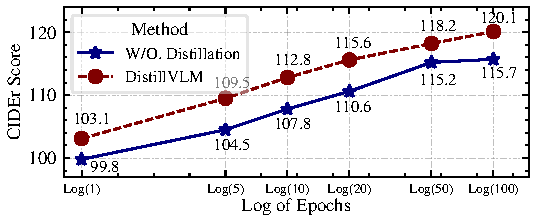
\includegraphics[width=.95\textwidth]{images/Effect_Epoch.pdf} 
    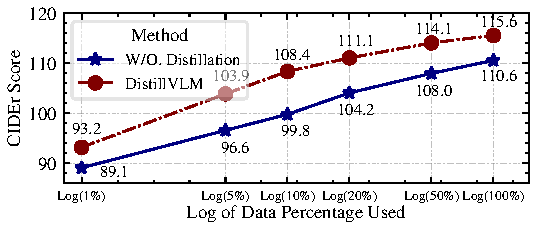
\includegraphics[width=.95\textwidth]{images/Effect_Data.pdf} 
    % \vspace{1mm}
    \caption[Captioning CIDEr scores gain from VL distillation under different epochs and portions of data.]{ Top: Captioning CIDEr score gain from VL distillation under different epochs ($1$, $10$, $20$, $50$, $100$) in  pre-training/distillation on VL-7M; Bottom: Using $1\%$, $10\%$, $20\%$, $50\%$ and $100\%$ of VL-7M image-text pairs with $20$ epochs of pre-training/distillation. }
    \vspace{-4mm}
    \label{fig:epoch} 
\end{figure}


\noindent We provide additional details of the VL distillation, which includes: a pseudo-implementation in PyTorch~\cite{paszke2017automatic} style; more results/ablations in the downstream; \distillvlm results transferred to the image retrieval task. To the end, we present qualitative analysis of attention distribution distillation and provide an analysis for VL Distillation and its broader impact for future studies.



\subsection*{Pseudo-implementation for VL Distillation}
The following section presents the pseudo implementation (see Page~\pageref{fig:pseudocode}) of our proposed VL distillation schema in \textit{Py}Torch style.


\subsection*{VL Distillation in Image Captioning Task}
We also conduct ablations of VL distillation in the task-specific fine-tuning stage. Table~\ref{tab:downablation} summarizes the fine-tuning results on image captioning task using different distillation losses, whereby weight loss parameters within the range of $[0, 1, 10]$ are searched for. All experiments are pre-trained/distilled for 20 epochs on the VL-7M dataset. In contrast to the results in pre-training stage VL distillation, we find that the $\mathcal{L}_\text{HID}$ and $\mathcal{L}_\text{att}$ do not contribute to the performances for downstream VL distillation. Instead, using just the $\mathcal{L}_\text{CLS}$ obviously improves the results: the CIDEr score is improved from $115.6$ to $116.3$.



\subsubsection*{Transferring to Image-text Retrieval Task}
In addition to the previously mentioned image captioning task and VQA task, \distillvlm is not VL task specific and can be extended to other tasks as well. In this section, we study whether the advantages from pre-training stage VL distillation extend to the image-text retrieval task on COCO dataset. In particular, the image-text retrieval task aims to retrieve the target image or text given a query text or image. We set up the image-text retrieval task on COCO dataset, and evaluate the performance of model using top-\textit{K} retrieval accuracy on both 1k and 5k test splits. To transfer and train the VL model for the image-text retrieval task, we use the first $\texttt{[CLS]}$ token from transformer in a binary classification task, where the classifier predicts whether the image and text match or not. To construct the negative tuple, irrelevant texts are sampled as non-matching cases. We fine-tune the model with learning rate at $2e-5$ and train it for $30$ epochs. The results are shown in Table~\ref{tab:retrieval}. 



\begin{table}[t!]
    \centering
    \setlength{\tabcolsep}{3.8pt} % Default value: 6pt
    \renewcommand{\arraystretch}{1.2} % Default value: 1
    \caption[Detailed distillation effects based on classification logit ($\mathcal{L}_\text{CLS}$), attention matrices ($\mathcal{L}_\text{ATT}$), hidden embedding ($\mathcal{L}_\text{HID}$).]{
    Detailed distillation effects based on classification logit ($\mathcal{L}_\text{CLS}$), attention matrices ($\mathcal{L}_\text{ATT}$), hidden embedding ($\mathcal{L}_\text{HID}$) with various weights ($\alpha$, $\beta$), compared with non-distilled strategy at fine-tuning stage. The first line shows the fine-tuning result without any distillation.
    }    
    { \small
    \begin{tabular}{ccc|cccc}
    \toprule
    \multirow{2}{*}{\textbf{$\mathcal{L}_\text{CLS}$}} & \multirow{2}{*}{\textbf{$\mathcal{L}_\text{ATT}$}} &  \multirow{2}{*}{\textbf{$\mathcal{L}_\text{HID}$}} & \multicolumn{4}{c}{{ COCO Captioning}}   \\ 
    & & & {B@4} & {M} & {C} & {S} \\
    \hline 
    $0$ & $0$ & $0$ & $34.6$ & $27.9$ & $115.6$ & $21.3$ \\
    $1$ & $0$ & $0$ & $34.6$ & $28.1$ & $116.3$ & $21.3$\\
    $1$ & $1$ & $0$ & $34.6$ & $28.1$ & $116.3$ & $21.3$ \\
    $1$ & $10$ & $0$ & $34.5$ & $28.0$ & $116.1$ & $21.3$ \\
    $1$ & $0$ & $1$ & $34.5$ & $28.0$ & $116.0$ & $21.3$ \\
    $1$ & $0$ & $10$ & $34.3$ & $28.0$ & $115.2$ & $21.2$ \\
    $10$ & $10$ & $10$ &  $34.6$ & $28.1$ & $116.4$ & $21.3$\\
    \bottomrule
    \end{tabular}
    }
    \label{tab:downablation}
\end{table}



\begin{table*}[t!]
\begin{center}
\renewcommand{\arraystretch}{1.2} % Default value: 1
\caption{Results of \distillvlm with and without VL distillation transferring to Image-Text Retrieval task  on COCO dataset.}
{
\scalebox{0.75}{
\begin{tabular}{lcc@{~~}c@{~~}cc@{~~}c@{~~}cc@{~~}c@{~~}cc@{~~}c@{~~}c}
\toprule
\hskip15pt \multirow{4}{*}{\textbf{Method}}  & & \multicolumn{6}{c}{\textbf{1K Test Set}} & \multicolumn{6}{c}{\textbf{5K Test Set}}     \\ 
\cmidrule(lr){3-8} \cmidrule(lr){9-14} & & \multicolumn{3}{c}{Text Retrieval}  & \multicolumn{3}{c}{Image Retrieval}   & \multicolumn{3}{c}{Text Retrieval}   & \multicolumn{3}{c}{Image Retrieval}  \\ [2px]
\cmidrule(lr){3-5} \cmidrule(lr){6-8} \cmidrule(lr){9-11}\cmidrule(lr){12-14} &    & R@1  & R@5  & R@10 & R@1 & R@5 & R@10  & R@1 & R@5 & R@10 & R@1 & R@5 & R@10  \\ 
\hline
PixelBERT & \xmark   & $77.8$  & $95.4$ & $98.2$ & $64.1$ & $91.0$ & $96.2$ & $53.4$ & $80.4$ & $88.5$ & $41.1$ & $69.7$ & $80.5$ \\  
Unicoder-VL& \xmark   & $84.3$  & $97.3$ & $99.3$ & $69.7$ & $93.5$ & $97.2$ & $62.3$ & $87.1$ & $92.8$ & $46.7$ & $76.0$ & $85.3$ \\
OSCAR$-\text{base}$& \xmark  & $88.4$  & $99.1$ & $99.8$ & $75.7$ & $95.2$ & $98.3$ & $70.0$ & $91.1$ & $95.5$ & $54.0$ & $80.8$ & $88.5$ \\ 
MiniVLM & \xmark &$81.1$  &$96.1$ & $99.2$   &$68.5$ &$93.0$  & $97.1$  &$58.8$  & $85.1$ & $91.7$ &$45.0$ &$74.1$   & $84.0$ \\ 
\hline
Baseline  & \xmark & $77.3$ & $95.0$  & $98.5$  & $64.6$ & $92.0$   & $96.7$ & $54.4$ & $81.4$  & $89.3$ & $41.3$ & $71.2 $ & $81.9$ \\
DistillVLM  & \checkmark & $80.0$ & $95.5$ & $98.5$ & $68.3$ & $92.3$ & $96.9$ & $58.3$ & $84.1$ & $91.3$ & $43.9$ & $73.7$ & $83.3$\\ [-5pt]
    \quad\enspace $\Delta$ & &  {\scriptsize$\mathcolor{darkgreen}{\textbf{+2.7}}$} &   {\scriptsize$\mathcolor{darkgreen}{\textbf{+0.5}}$} &   {\scriptsize{+0.0}} &   {\scriptsize$\mathcolor{darkgreen}{\textbf{+3.7}}$} &  {\scriptsize$\mathcolor{darkgreen}{\textbf{+0.3}}$} & {\scriptsize$\mathcolor{darkgreen}{\textbf{+0.2}}$} &   {\scriptsize$\mathcolor{darkgreen}{\textbf{+3.9}}$} &   {\scriptsize$\mathcolor{darkgreen}{\textbf{+2.7}}$} &   {\scriptsize$\mathcolor{darkgreen}{\textbf{+2.0}}$} &   {\scriptsize$\mathcolor{darkgreen}{\textbf{+2.6}}$} &   {\scriptsize$\mathcolor{darkgreen}{\textbf{+2.5}}$} &   {\scriptsize$\mathcolor{darkgreen}{\textbf{+1.4}}$}\\

\bottomrule
\end{tabular}
}}
\label{tab:retrieval}
\end{center}
\end{table*}




\begin{table}[t!]
    \centering
    \setlength{\tabcolsep}{4.5pt} % Default value: 6pt
    \renewcommand{\arraystretch}{1.2} % Default value: 1
    \caption[Effect of VL distillation with and without Teacher VLM adaptation in pre-training stage.]{
    Effect of VL distillation with and without Teacher VLM adaptation in pre-training stage. First row in the table shows the captioning performances using VL pre-training without VL distillation. $^{\color{red} *}$ denotes the VL distillation results without re-training the Teacher VLM.
    }    
    { \small
    \begin{tabular}{c|cccc}
    \multirow{2}{*}{\textbf{Method}} & \multicolumn{4}{c}{{COCO Captioning }} \\ 
    & {B@4} & {M} & {C} & {S} \\
    \hline
    VL Pre-training & $33.0$ & $27.3$ & $110.6$ & $20.4$ \\
    VL Distill. w/o. Adaptation & $33.3$ & $27.5$ & $112.3$ & $20.6$ \\
    VL Distill. with Adaptation.$^{\color{red} *}$ &  $34.4$ & $27.9$ & $115.0$ & $21.0$\\
    VL Distill. with Adaptation & $34.6$ & $27.9$ & $115.6$ & $21.3$ \\

    \end{tabular}
    }
    \label{tab:vlpadapt1}
\end{table}

\begin{table}[t!]
    \centering
    \setlength{\tabcolsep}{5.pt} % Default value: 6pt
    \renewcommand{\arraystretch}{1.2} % Default value: 1
    \caption[Effect of VL distillation with and without Teacher VLM adaptation in fine-tuning stage.]{
    Effect of VL distillation with and without Teacher VLM adaptation in fine-tuning stage. First row in the table shows the COCO captioning results without any downstream distillation.
    }    
    { \small
    \begin{tabular}{c|cccc}
    \multirow{2}{*}{\textbf{Method}} & \multicolumn{4}{c}{{COCO Captioning}} \\
    & {B@4} & {M} & {C} & {S} \\
    \hline 
    VL Pre-training & $33.0$ & $27.3$ & $110.6$ & $20.4$ \\
    VL Distill. w/o. Adaptation & $33.2$   & $ 27.5$ & $110.7$  & $20.3$\\
    VL Distill. with Adaptation & $33.5$ & $27.5$ & $111.6$ & $20.6$\\
    \end{tabular}
    }
    \label{tab:vlpadapt2}
\end{table}

We just examine the effect of VL distillation in the pre-training stage. 
DistillVLM without VL distillation is notably worse than MiniVLM: $81.1$ \vs $77.3$ accuracy of R@$1$ on 1$K$ Test Set,  since less training data is used. Equipped with pre-training stage VL distillation, it is significantly improved to $80.0$ and $58.3$ accuracy of R@$1$ on $1$K/$5$K Test Set respectively, which are $2.7$ and $4.0$ higher. Compared to its counterpart MiniVLM~\cite{wang2020minivlm} and other state-of-the-art methods, \distillvlm achieves on par performances, while MiniVLM is trained on 14M image-text pairs, which is twice the size of our pre-training VL corpus. Other methods all use a larger transformer model or stronger visual representations. 


\subsubsection{Discussion on Teacher VLM Adaptation}


\begin{table*}[t!]
    \centering
    \setlength{\tabcolsep}{7pt} % Default value: 6pt
    \renewcommand{\arraystretch}{1.2} % Default value: 1
    \caption[Detailed image captioning results for data efficient VL distillation.]{ Detailed image captioning results for data efficient VL distillation. The rows in gray show results using non-distilled VL pre-training method, and the following rows show results with VL distillation.}    
    { \small
    \begin{tabular}{ccccc|ccccc}
    % \toprule
    \multirow{2}{*}{{\# \textit{Epochs}}} & \multicolumn{4}{c|}{{ COCO Captioning}} & \multirow{2}{*}{{\% \textit{Data}}} & \multicolumn{4}{c}{{ COCO Captioning}} \\ 
    &  {B@4} & {M} & {C} & {S}  & &   {B@4} & {M} & {C} & {S} \\ 
    \hline
    % \rule{0pt}{1.03\normalbaselineskip}
    \rowcolor{gray!15}\multirow{2}{*}{{ {1}}} & $31.3$ & $25.6$  & $99.8$ & $19.0$ & \multirow{2}{*}{{ {1\%}}} & $27.9$  & $24.2$  & $89.1$ & $17.2$ \\
    & $31.3$  & $26.2$  & $103.3$ & $19.4$ & & $29.2$  & $24.6$  & $93.2$ & $17.8$ \\
    \hline
    \rowcolor{gray!15}
    \multirow{2}{*}{{ {5}}} & $31.3$  & $26.4$  & $104.5$ & $19.6$ & \multirow{2}{*}{{ {5\%}}} & $29.5$  & $25.1$  & $96.6$ & $18.4$ \\
    & $32.8$  & $27.3$  & $109.5$ & $20.5$ & & $31.6$  & $26.3$  & $103.9$ & $19.3$ \\
    \hline
    \rowcolor{gray!15}
    \multirow{2}{*}{{ {10}}} & $32.2$  & $26.8$  & $107.8$ & $20.2$ & \multirow{2}{*}{{ {10\%}}} & $30.2$  & $25.7$  & $99.8$ & $18.9$ \\
    & $33.9$  & $27.5$  & $112.8$ & $20.6$ & & $32.8$  & $27.0$  & $108.4$ & $20.0$ \\
    \hline
    \rowcolor{gray!15}
    \multirow{2}{*}{{ {20}}} & $33.0$  & $27.3$  & $110.6$ & $20.4$ & \multirow{2}{*}{{ {20\%}}} & $31.2$  & $27.3$  & $104.1$ & $19.6$ \\
    & $34.6$ & $27.9$ & $115.6$ & $21.3$ & & $33.4$  & $27.3$  & $111.1$ & $20.5$ \\
    \hline
    \rowcolor{gray!15}
    \multirow{2}{*}{{ {50}}} & $34.3$  & $27.8$  & $115.2$ & $21.1$ & \multirow{2}{*}{{ {50\%}}} & $32.2$  & $26.9$  & $108.5$ & $20.1$ \\
    & $35.1$  & $28.2$  & $118.2$ & $21.5$ & & $34.0$  & $27.7$  & $114.1$ & $21.2$ \\
    \hline
    \rowcolor{gray!15}
    \multirow{2}{*}{{ {100}}} & $34.0$  & $28.0$  & $115.7$ & $21.1$ & \multirow{2}{*}{{ {100\%}}} & $33.0$  & $27.3$  & $110.6$ & $20.4$ \\
    & $35.2$ & $28.6$ & $120.1$  & $21.9$ & & $34.6$  & $27.9$  & $115.6$ & $21.3$ \\
    % \bottomrule
    \end{tabular}
    }
    \label{tab:efficient}
\end{table*}

Unlike the previous knowledge distillation where the Teacher model is usually not re-trained, Teacher VLM in our work is adapted using the new visual tokens. This is to ensure that the use of new Teacher visual tokens does not have a negative impact to the Teacher. Nevertheless, it is also viable to use Teacher VLM directly without adaptation. We compare the performances using Teacher VLM with and without adaptation in Table~\ref{tab:vlpadapt1} and~\ref{tab:vlpadapt2} in both pre-training and fine-tuning stages. 

In particular, we first conduct VL distillation in pre-training stage without using the adapted Teacher VLM, and use the old visual tokens as in~\cite{li2020oscar} without re-extracting them using object proposals from the lightweight detector. As there is no semantic correspondence across Teacher and Student's tokens, we just adopt the classification distillation on the masked tokens' logit. The second line of Table~\ref{tab:vlpadapt1} gives the results (VL Distill. w/o. Adaptation), where we observe a slight improvement on captioning performances: $112.3$ \vs $110.6$. Furthermore, we apply the visual tokens extracted according to the Student detector's object proposals, which guarantees the semantic correspondence across Teacher and Student tokens. With that, we conduct the VL distillation using the our proposed losses ($\mathcal{L}_\text{ATT}$ and $\mathcal{L}_\text{HID}$), and find significant improvement: CIDEr score increases from $110.6$ to $115.0$ (as shown in third line of Table~\ref{tab:vlpadapt1}). Finally, by re-training the Teacher VLM using the new extracted visual tokens will lead to more improvement: $115.6$ \vs $115.0$. This confirms that, even without re-training the Teacher VLM, VL distillation still gives satisfactory results.

We conduct similar investigations in the downstream and show results in Table~\ref{tab:vlpadapt2}. In particular, downstream VL Distillation without adaptation gives minor improvement ($0.2$ and $0.1$ for BLEU@$4$ and CIDEr scores), while using the adapted Teacher VLM leads to obvious better results ($0.5$ and $1.0$ higher on BLEU@$4$ and CIDEr score). We only apply the classification distillation loss in the downstream experiments.


\subsection*{Detailed Results for Data Efficient VL Distillation }
Table~\ref{tab:efficient} summarizes more detailed results of data efficient VL distillation on image captioning tasks.  In particular, we compare the effectiveness of  VL distillation in pre-training stage using different converging epochs $[1, 5, 10, 20, 50, 100]$ and fraction data $[1\%, 5\%, 10\%, 20\%, 50\%, 100\%]$.  VL distillation comprehensively improves the results on all metrics, regardless of the amount of data available or different training epochs.



% \section*{Effect of Attention Distribution Distillation}
% \label{sec:adapt}
% In Figure~\ref{fig:att}, we show qualitative effect of attention distribution distillation where we select random samples from VL corpus and retrieve their last transformer block attention maps from the Teacher VLM, \distillvlm and the non-distilled counterpart of \distillvlm. To illustrate this, the attention maps are averaged over 12 self-attention heads. Based on the examples, we observe that the attention maps after VL distillation exhibit higher similarities to the Teacher VLM's attention maps. This confirms that our attention distribution distillation successfully mimic the Teacher VLM's attention distribution to some extent.

\label{fig:pseudocode}
{\centering
    \lstset{
        language={python},
        % backgroundcolor=\color{backcolor},  
        commentstyle=\color{darkgreen}\ttfamily,
        commentstyle=\color{darkgreen},
        keywordstyle=\color{magenta},
        numberstyle=\tiny\color{maroon},
        stringstyle=\color{codepurple},
        basicstyle=\ttfamily\footnotesize,
        breakatwhitespace=false,         
        breaklines=true,                 
        captionpos=b,                    
        keepspaces=true,                 
        numbers=left,                    
        numbersep=1pt,                  
        showspaces=false,                
        showstringspaces=false,
        showtabs=false,                  
        tabsize=2,
        moredelim=**[is][\color{maroon}]{<}{>},
        moredelim=**[is][\color{blue}]{--}{--},
        moredelim=**[is][\color{maroon}]{```}{```},
        moredelim=**[is][\color{p}]{---}{---},
    }
    \begin{lstlisting}
    ```--Q:-- Maintaining queue of random history representations: (---K--- X ---DT---)
    --teacher_model, student_model:-- Large/small Teacher/Student VL model. 
    --FC--: Linear layer for dimension transformation of student hidden representation.
    --temp:-- Temperatures of the NCE loss.
    --lamda, beta--: Weights for loss terms.
    ```
    
    # activate evaluation mode for Teacher to freeze BN and updation.
    with torch.no_grad():
        # t_atts: 1 X N X N, t_hids: 1 X N X DT
        t_atts, t_hids = --teacher_model--(**teacher_inputs)
    
    # s_atts: 1 X N X N, s_hids: 1 X N X DS
    mlm_loss, itm_loss, s_atts, s_hids = --student_model--(**student_inputs)
    
    # dimension transformation on student hidden, s_hids: 1 X N X DT
    s_hids = --FC--(s_hids)
    
    # attention distillation loss
    att_loss = <mse_loss>(s_atts, t_atts)

    # NCE hidden states distillation loss
    
    # l2-norm the hidden representation
    t_hids, s_hids = <L2_norm>(s_hids), <L2_norm>(t_hids)

    # positive logit: Nx1
    l_pos = torch.<einsum>('nd,nd->n',  [s_hids.squeeze(0), t_hids.squeeze(0)])

    # negative logit: NxK
    l_neg = torch.<einsum>('nd,dk->nk', [s_hids.squeeze(0), Q.<detach>().<T>()])

    # logit: Nx(1+K)
    logits = torch.<cat>([l_pos, l_neg], dim=1)

    # apply the temperature for NCE loss
    logits /= --temp--

    # NCE label: N
    labels = torch.<zeros>(logits.shape[0], dtype=torch.long).cuda()

    nce_loss = <ce_loss>(logits, labels)

    # update the queue with current teacher hidden states.
    <dequeue_and_enqueue>(t_hids, Q)
    
    # aggregated losses
    loss = mlm_loss + itm_loss + --lamda-- * att_loss + --beta-- * nce_loss
    \end{lstlisting}
}
% \caption{Our VL distillation consists of the attention distribution and hidden embedding mimicking when batch size $= 1$ with $N$ textual/visual tokens. We assume \texttt{[PAD]} tokens are excluded from input tokens before the distillation. }




% \begin{figure*}
% \centering
% \begin{subfigure}{.5\textwidth}
%   \centering
%     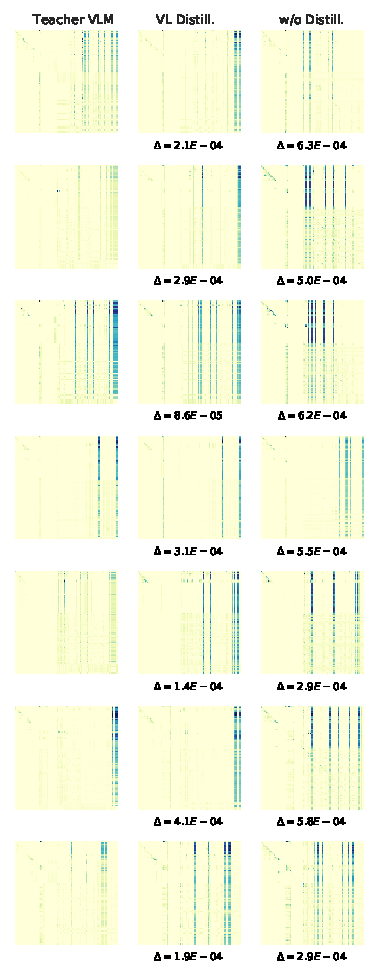
\includegraphics[width=.9\textwidth]{images/a.pdf} 
%   \label{fig:sub1}
% \end{subfigure}%
% \begin{subfigure}{.5\textwidth}
%   \centering
%     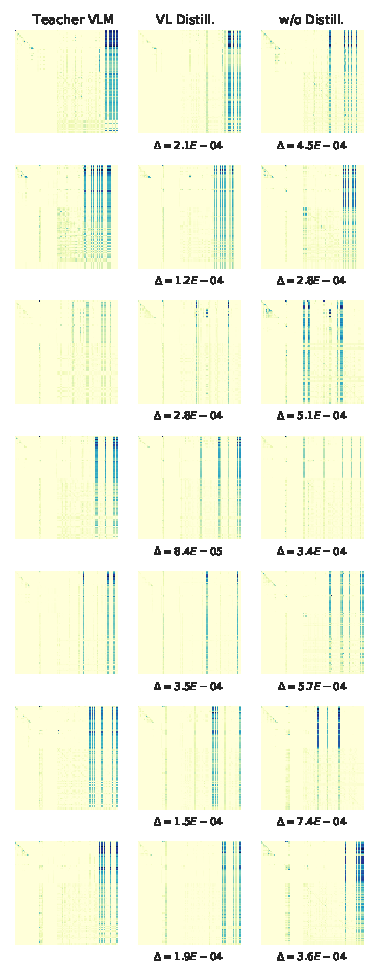
\includegraphics[width=.9\textwidth]{images/b.pdf} 
%   \label{fig:sub2}
% \end{subfigure}

% \caption{\small Qualitative effect of attention distribution distillation. The 3 neighbouring attention maps are the averaged attention map from the last transformer block of: Teacher VLM, \distillvlm, and non-distilled VL model. The number at bottom is the $l2$ distance of the attention map with its corresponded Teacher attention map.}
% \label{fig:att}
% \end{figure*}

\subsection{Conclusion}
We have proposed the first VL distillation, which leverages the knowledge distillation technique to compress large visual-linguistic models. Our experiments confirmed the validity of VL distillation from several aspects: Compared to the non-distilled VL pre-training method, VL distillation not only brings better performances, it is also more data efficient. Our extensive ablations also verified that our VL distillation strategies are simple yet effective.



% % \chapter{Towards One-stage Image Captioning Model}
\chapter{TOWARDS ONE-STAGE IMAGE CAPTIONING MODEL}

The task of image captioning aims to generate human-readable descriptive text from an image. Recent studies have witnessed its great development which are primarily reflected in the aspects of more advanced cross-modal fusion architectures~\citep{you2016image,vinyals2015show, xu2015show,rennie2017self,yang2019auto,cornia2020meshed,pan2020x,ting2019hierarchy,zhang2021rstnet}; more expressive object-centric features~\citep{anderson2018bottom,zhang2021multi} \& tags~\citep{li2020oscar,hu2020vivo,wang2020minivlm,fang2021compressing} obtained from a pre-trained object detection model; or learning general \textbf{\textit{V}}ision and \textbf{\textit{L}}anguage (VL) representations from large image-text corpus~\citep{zhou2020unified,xu2021e2e,li2020oscar,wang2021simvlm,wang2020minivlm,fang2021compressing}.

\begin{figure}[t!]
 \vspace{-3mm}
  \begin{center}
    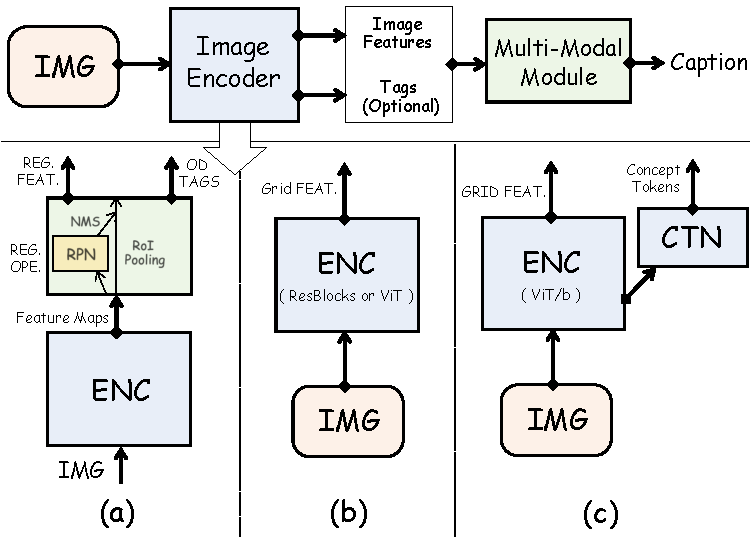
\includegraphics[width=.76\textwidth]{./images/vit_cap.pdf} 
  \end{center}
  \vspace{-5mm}
    \caption[Comparisons of different image captioning models.]{\small \textbf{Comparisons of different image captioning models}. Top: A general image captioning pipeline. Bottom: (a). Prevailing conventional models~\citep{li2019scale,zhang2021multi,hu2020vivo} which are based on an object detector to extract regional features. 
    Object tags~\citep{li2020oscar,zhang2021multi} can be optionally used to assist the text generation through a multi-modal decoder network. This usually requires regional operations (REG. OPE.) that are time consuming.
    (b). To eliminate the detection module, a ResNet variant~\citep{he2016deep} or Vision Transformer~\citep{kim2021vilt} can be applied as substitution to output the grid feature~\citep{xu2021e2e,wang2021simvlm}. 
    This replacement has been studied on the image understanding task recently but very few works
    focus on the generation task. 
    (c). Our proposed \vitcapp\!\!, which is detector-free and incorporates a novel Concept Token Network
    to predict semantic concepts as tokens for the image captioning task.
    }
    \vspace{-2mm}
  \label{fig:abstract}
\end{figure}

Despite these significant advances, most of the mainstream captioning models~\citep{cornia2020meshed,pan2020x,ting2019hierarchy,zhang2021rstnet} rely heavily on a bulky object detector to provide regional visual representations for the multimodal interaction, as shown in Figure~\ref{fig:abstract}-a. 
In spite of the superior performance brought by the object features, 
the ensuing difficulties occur as they: 1) \textbf{lead to heavy computational load} due to the regional operations (\ie, RPN, RoI Pooling, and NMS). These intermediate operations unavoidably cause training inefficiency and high inference latency at prediction stage~\citep{kim2021vilt,wang2020minivlm}; 2) \textbf{require box annotations} and largely limit the flexibility in training and application;  
% 3) are \textbf{unable to update the visual features} from the detector which are not directly optimized towards generating high quality image captions~\citep{xu2021e2e}. 
To address these challenges, there is an emerging trend that more recent works propose to eliminate the detector for the VL pre-training in an end-to-end fashion~\citep{jiang2020defense,huang2020pixel,kim2021vilt,yan2021grid,wang2021simvlm}. In such detector-free design, a general visual encoder serves as a substitute for the detector and from which the grid features are produced for later cross-modal fusion, as in Figure~\ref{fig:abstract}{\color{black}-b}.
Heretofore, the majority of these works mainly focus on the image understanding task, which is typically cast as a classification problem, and only a few of them shed light on the generation task.
In~\citep{xu2021e2e}, the image is encoded with ResNet~\citep{he2016deep} and 
the performance ($117.3$ CIDEr on COCO~\citep{xu2021e2e})
is still far from the state-of-the-art detector-based approach ($129.3$ CIDEr with VinVL-base~\citep{zhang2021multi}).
% with moderate VL training corpus ($6$ million image-text pairs),
% Recent work of SimVLM~\citep{wang2021simvlm} boosts the performance significantly but with as large as $1.8$ billion image-text pairs, which is inaccessible for public. 
% In the meantime, we observe that the currently existing endeavors for the image captioning task are still far from reaching on par outcomes of the detector-based methods, from either the perspective of performance~\citep{xu2021e2e} or training efficacy (\eg, \citep{wang2021simvlm} exploits a massively larger VL corpus than the previous). 
The challenge remains uncharted and insufficiently investigated regarding \textit{how to build a stronger detector-free image captioning model.}
% (\eg, E2E-VLP reaches only $117.3$ CIDEr scores on COCO-caption compared with $123.7$ from~\citep{li2020oscar})


Previous efforts~\citep{li2020oscar,hu2020vivo,zhang2021multi,wang2020minivlm,fang2021compressing} have demonstrated that the object tags play an important role in improving the captioning performance. 
Instead of gleaning the object tags from the detector, we introduce a novel fully \textbf{VI}sion \textbf{T}ransformer based image \textbf{CAP}tioning model, dubbed ViTCAP, with a lightweight Concept Token Network (CTN) that produces concept tokens (see Figure~\ref{fig:abstract}{\color{black}-c}). 
ViTCAP is constructed on the basis of a vision transformer~\citep{dosovitskiy2020image} as the stem image encoder. Our vision transformer backbone starts with encoding the image and produces grid features, on top of which the CTN branch is then applied to predict semantic concepts of images. We represent the semantic concepts at the token level instead of the tag level to avoid the tokenization. 
The multi-modal module then takes the input of both grid representations and Top-$K$ concept tokens for decoding. During training, the CTN is optimized to predict the pseudo ground-truth concepts extracted from image captions via a simple classification task. We also investigate to adopt the object tags from the detector as the pseudo ground-truth, and empirically observe no further improvement. Overall, this straight-forward design allows the injection of semantic concepts into the multi-modal fusion module with abundant semantics, and is critical for the improved captioning performance.

Our ablative analysis suggests that, with no bells and whistles, simple vanilla transformer architecture based \vitcap 1) significantly outperforms existing detector-free captioning models;
%2) surpasses most detector-based models and approaches on par performances with staste of the arts. 
2) surpasses most detector-based models and 3) approaches the state-of-the-art detector-based models. 
% with great inference speed improvement on multiple image captioning benchmarks.
In particular, \vitcap achieves $138.1$ CIDEr scores on COCO-caption Karpathy split~\citep{lin2014microsoft}, $108.6$ on Google-CC~\citep{sharma2018conceptual}, and $95.4$ on nocaps~\citep{agrawal2019nocaps} datasets.

\noindent To summarize our contributions:
\begin{itemize} [leftmargin=8pt]
    \item We present a detector-free image captioning model  \vitcap\!\! with fully transformer architecture, where it leverages grid representations without regional operations. 
    \item We propose to inject semantic concepts into end-to-end captioning by learning from open-form captions. We find that our proposed concept classification training and concept tokens significantly benefit the captioning task.
    \item Extensive evaluations on multiple captioning datasets confirm the validity of our method. \vitcap achieves competitive or even leading results amongst detector-based prior arts with clear inference-time advantages.
\end{itemize}


\subsection{ViTCAP}
% Vision Transformer for Image Captioning
Existing image captioning models usually consist of an object detector module (\textbf{Detector}) to extract regional feature ($\vv^{T}$) from the raw image (\,$\mathbf{I}$\,), and a multi-modal module (\textbf{MM}) to generate a textual description (\,$\vc$\,). Several recent works~\citep{li2020oscar,zhang2021multi} show that the object tags ($\vt^{T}$) extracted from the detector can serve as anchoring points across modalities, and are essential for various VL tasks. This procedure can be expressed as follows:
\begin{equation}
    (\vv^{T}, \vt^{T}) = \text{\textbf{Detector}}(\, \mathbf{I}\,), \cv = \text{\textbf{MM}}(\vv^{T}, \tv^{T}).
\end{equation}
Several VL models~\citep{huang2020pixel,kim2021vilt,xu2021e2e} obtain a great improvement in inference speed by using general image encoders without regional operations. However, these models are unable to utilize the image tags due to the absence of a detector.  

In this work, we aim to build a detector-free captioning model with concept tokens containing rich semantics, coming from a novel Concept Token Network (CTN).
An overview of \vitcap is depicted in Figure~\ref{fig:architecture}. 
The raw image is firstly fed into the image encoder to generate the intermediate representations ($\vv_{i}$) and the final grid representations ($\vv$).
% \vitcap consists of an image encoder module that produces an grid representations ($\vv$),
A CTN branch then takes $\vv_{i}$ as the input and predicts concept tokens ($\tv$), followed by the multi-modal module that allows the interactions across modalities and generates caption ($\cv$). We adopt the fully transformer~\citep{vaswani2017attention} framework in all modules, but the image encoder and CTN modules are not architecture-specific. The overall pipeline can be summarized as:
% \text{\textbf{M}}^{2}\text{-}\, \text{\textbf{Mod.}}
\begin{equation}
    (\!\vv_{i}, \vv\!) \!=\! \text{\textbf{Encoder}}(\, \mathbf{I}\,), \ \ \tv \! = \! \text{\textbf{CTN}}(\vv_{i}), \ \ \cv \! = \! \text{\textbf{MM}}(\vv, \tv).
\end{equation}
In the following, we first introduce how the vision transformer produces grid representations and our proposed CTN in Section~\ref{sec:tagger}, and the overall training losses in Section~\ref{sec:training}.


 
\subsubsection{Model Structure}
% \subsubsection{Vision Transformer}
\noindent \textbf{Vision Transformer.}
\label{sec:vit}   % its okay to release some space here.
The transformer architecture and its instantiations (\eg, BERT~\citep{devlin2018bert}, GPT~\citep{brown2020language}) are well-known for their remarkable performances on natural language processing tasks, which are mostly attributed to the self-attention design. Recent efforts have advanced this to vision tasks, \ie, Vision Transformer (ViT)~\citep{dosovitskiy2020image}. 
We use ViT as the backbone of the image encoder to produce grid representations ($\vv_i$ and $\vv$ ). 
% To be specific, the raw image $\mathbf{I}\in\mathbb{R}^{H\times W \times3}$ is partitioned into $N$ disjoint patches with each in the size of $P\!\times\!P\!\times\!3$, $N\!=\frac{H\times W}{P\times P}$. 
To be specific, the raw image $\mathbf{I}\in\mathbb{R}^{H\times W \times3}$ is partitioned into $N$ disjoint patches. The size of each patch is $P\!\times\!P\!\times\!3$ and the number of patches $N\!$ is 
% $\frac{H\times W}{P\times P}$. 
${(H W)}/{P^2}$. 
% These patches are then flattened and projected into patch embedding of dimension $d$ via a trainable linear projection layer, feeding into consecutive transformer blocks thereafter. 
These patches are then flattened and projected into patch embedding of dimension $d$ via a trainable linear projection layer. Concatenated with a special \texttt{[CLS]} token, these patch representations are added with learnable positional embeddings and then sent into $M$ consecutive transformer blocks thereafter. 
To this end, we use the final representation as the grid features $\vv$, and extract the output of the first $M_1$ blocks as the intermediate representations $\vv_i$, which is the input of the Concept Token Network for concept predictions as detailed below. 
% To this end, grid representations $\vv_i, \vv\in\mathbb{R}^{(N+1)\times d}$ of the image are produced for decoding, with one additional feature for the \texttt{[CLS]} token. $\vv_i$ and $\vv$ are intermediate and final grid representations produced from the stem image encoder and feature extractor.
% The CTN is built upon the initial $M_1$$ transformer blocks with the image encoder (stem image encoder as in Figure~\ref{fig:architecture}), which saves the computational cost with minor performance loss. We experiment with a different number of sharing blocks and compare their results in ablations.
% The intermediate grid representations $\vv_{i}\in\mathbb{R}^{(N+1)\times d}$ are produced from the stem image encoder for the CTN branch. 

\vspace{1mm}
\noindent \textbf{Concept Token Network.}
% \subsection{Concept Token Network}
\label{sec:tagger}
The Concept Token Network (CTN) is composed of $M_2$ transformer blocks to process the intermediate
features $v_i$. The output representation corresponding to \texttt{[CLS]} is used to predict the 
concept token with a multi-linear perceptual (MLP) network. 
The vocabulary of the concept token is identical with the one used for the captions. 
It is noted that we predict the concept in the token level rather than in the tag level, and thus the top-$K$ ($K=50$ in our experiments) tokens can be directly used by the multi-modal decoding module for auto-regressive decoding. In~\citep{li2020oscar,zhang2021multi}, the object tags are predicted from the object detector, while we eliminate the detection module to remove the dependency of the box annotations. Another difference lies in the tag/concept vocabulary. The existing approaches apply the tag list from the dataset as the vocabulary which are pre-defined and need an extra tokenization operation. Instead, our concept token vocabulary is shared with the one for captions and also removes the tokenization step.

% to avoid the 
% tokenization operation. 

% Heretofore, most existing VL models rely on the object detector to retrieve expressive regional features and object tags~\citep{li2020oscar,zhang2021multi} as the anchor points. These categorical tags are known to implicitly align between text and the regional features, thus beneficial for VL tasks. We propose to build a Concept Token Network on top of the stem image encoder, where the CTN predicts semantic concepts through a classification task. In practice, our CTN consists $M-M_1$ transformer blocks to guarantee a consistent 

% We formulate the concept token learning process as a $K$-way classification task using the \texttt{[CLS]} token embedding after a classification head consisting of two linear projection layers. When proceeding to the decoding module, we simply retain the embeddings of the top-$K$ concepts from the vocabulary as concept tokens $\tv$. This exempts us from the operation of tokenization during captioning, and differs from how object tags are encoded as in previous VLP works~\citep{li2020oscar,zhang2021multi}.
% Details of CTN training are discussed in later sections.



\vspace{1mm}
\noindent \textbf{Multi-Modal Fusion Module.}
% \subsection{Multi-modal Module for Decoding}
\label{sec:multimodal}
% Our multi-modal fusion module is a shallow network composed of multiple transformer blocks. 
% % During decoding, we first adopt the Top-$K$ concept tokens' indexes to retrieve their corresponded token embedding from the caption embedding layer as concept token embedding $\tv$. 
% During decoding, the Top-$K$ concept tokens' indexes is mapped to token embeddings through an embedding layer, which is shared with the caption embedding layer.
% Then, the module takes as input the concatenation of concept token embedding and grid representations $(\tv, \vv)$. And during decoding, the multi-modal module produces the caption $\cv$ in an auto-regressive manner given the first \texttt{[CLS]} token. % During decoding, we first adopt the Top-$K$ concept tokens' indexes to retrieve their corresponded token embedding from the caption embedding layer as concept token embedding $\tv$. 
Our multi-modal fusion module is a shallow network composed of multiple transformer blocks, and we follow~\citep{radford2018improving,brown2020language} to apply the \texttt{seq2seq} attention mask to generate the caption token in an auto-regressive way.
First, the Top-$K$ concept tokens' indices are mapped to token embeddings through an embedding layer $l_c$.
Then, the module takes as input the concatenation of concept token embeddings ($\tv$) and grid representations ($\vv$) to generate the description, where we append a mask token \texttt{[MASK]} to the previous generated tokens (empty at very beginning) to predict the next token one by one.
With the \texttt{seq2seq} attention mask, the generated token (including the appended \texttt{[MASK]} token) is able to access the preceding tokens and $(\tv, \vv)$, while $(\tv, \vv)$ has no access to the generated tokens.  
The generated caption token is also mapped through an embedding layer $l_d$.
In experiments, we make the two embedding layers ($l_c$ and $l_d$) shared to reduce the parameter size as the result is similar to two separate layers. 
% Empirically, we observe that the results are similar when $l_c$ and $l_d$ are shared or not (see Appendix for results). To reduce the parameter size, we use the shared embedding layer for both steps. For the auto-regressive decoding, we also have an embedding layer $l_d$ to map the generated token which is shared with the caption embedding layer





\begin{figure*}[t!]
  \begin{center}
    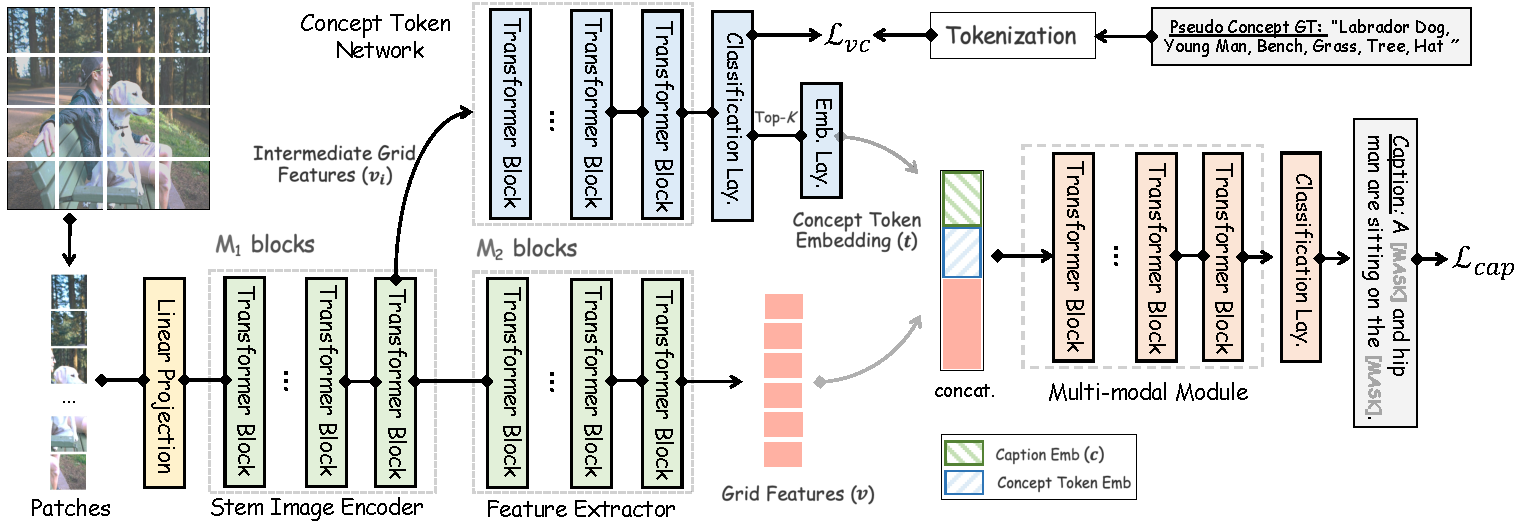
\includegraphics[width=\textwidth, height=0.35\textwidth]{./images/vitcap_architecture.pdf}
    \vspace{-8mm}
  \end{center}
    \caption[Architecture of our proposed \vitcapp image captioning model]{\small \textbf{Architecture of our proposed \vitcapp image captioning model}. \vitcapp is a detector-free image captioning model based on the vision transformer, where image patches are encoded into continuous embeddings as grid representations. The CTN branch roots from an intermediate block of the image encoder, and is a shallow transformer architecture (\eg, 4 self-attention blocks). The CTN is trained via a classification task using object tags gleaned from the Teacher VLM's detector as pseudo-labels and the keywords parsed from image captions as the semantic concept ground-truth. During captioning, the CTN-produced concept tokens from the semantic concept vocabulary are then concatenated with the grid representations and fed into the multi-modal module for decoding. Best viewed in color.
    }
  \label{fig:architecture}
  \vspace{-3mm}
  \end{figure*}

\subsection{Model Training}
\label{sec:training}
The training of \vitcap is composed of the CTN and the captioning training.
% , where the CTN learns to predict existed image-level concepts.
% We jointly optimize both multi-modal module and the TCN branch as the pre-trained TCN can be further adapted at the captioning dataset.
% In order to inject broad semantic concepts into the model, we use the caption extracted keywords (including nouns and adjective words) as the pseudo ground-truth concepts. 
% An alternative way to retrieve the target concepts is to leverage the detector-produced image tags. We also experiment with the object detector pre-trained on Visual Genome~\citep{krishna2017visual} to generate categorical tags as the image-level pseudo-labels for training but find no better results. This is because though such detectors are capable of recognizing diverse collections of semantic concepts, they are largely limited because of the pre-defined categories based on the pre-training dataset. Learning from open-form captions gives much richer concepts, while adopting the detector-produced tags as pseudo-labels allows flexible training when image captions are not attainable. 
CTN is used to predict the image concepts. However, the widely-used VL pre-training dataset contains only the image descriptions without the tags. To address the issue, one can simply retrieve the concepts from the open-form captions (\eg, by extracting nouns or adjective words as keywords) as the pseudo ground-truth concepts, or alternatively leverage a pre-trained object detector (\eg on Visual Genome~\citep{krishna2017visual}) to produce the image tags (remove the bounding boxes). Empirically, we observe that by using caption extracted concepts lead to better results.
% The training of \vitcap is composed of the CTN and the captioning training, where the CTN learns to predict existed image-level concepts.
% % We jointly optimize both multi-modal module and the TCN branch as the pre-trained TCN can be further adapted at the captioning dataset.
% In order to inject broad semantic concepts into the model, we use the caption extracted keywords (including nouns and adjective words) as the pseudo ground-truth concepts. 
% An alternative way to retrieve the target concepts is to leverage the detector-produced image tags. We also experiment with the object detector pre-trained on Visual Genome~\citep{krishna2017visual} to generate categorical tags as the image-level pseudo-labels for training but find no better results. This is because though such detectors are capable of recognizing diverse collections of semantic concepts, they are largely limited because of the pre-defined categories based on the pre-training dataset. Learning from open-form captions gives much richer concepts, while adopting the detector-produced tags as pseudo-labels allows flexible training when image captions are not attainable. 
% we experiment with different sources of semantic concepts as learning targets: 1). the detector-produced image tags, and 2). keywords extracted from the descriptive image captions as target concepts. 
% We leverage the object detector pre-trained on Visual Genome~\citep{krishna2017visual} to generate categorical tags as the image-level pseudo-labels for training. Even though such detectors are capable of recognizing diverse collections of semantic concepts, they are largely limited because of the pre-defined categories based on the pre-training dataset. covering extensive objects and visual attributes. 
% % By concatenating both the object labels and attribute labels as VinVL for a more diverse collection of semantic concepts, covering $1,848$ object categories and $524$ attribute categories. 
% To further broaden the semantic concepts, we expand the taxonomy of semantic concepts by extracting keywords from image captions. Though learning from open-form captions gives much richer concepts, adopting the detector-produced tags as pseudo-labels allows flexible training when image captions are not attainable.
We optimize the CTN to predict the target concepts via a multi-label classification task. Due to the extremely imbalanced semantic concepts distribution (certain concepts appear much frequently than the rest), we adopt the simplified asymmetric focal loss~\citep{ben2020asymmetric,liu2021query2label,lin2014microsoft} which shows great performances handling sample imbalance problems for the multi-label classification task. The overall concept classification loss can be expressed as: 
%  \ \ \  \text{where} \ \
\begin{align}
\mathcal{L}_{{vc}} = \mathbb{E}_{\vv_i\sim D}f_{\theta}(p\ |\ \vv_i),
\end{align}
% and the objective $f_{\theta}(p\ |\ \vv_i)$ is:
\begin{equation}
      f_{\theta}(p\ |\ \vv_i) = \frac{1}{K} \sum^{K}_{k=1}
\begin{cases}
    (1-p_{k})^{\gamma_{+}}\cdot\text{log}(p_k), & +, \\ p_{k}^{\gamma_{-}} \cdot \text{log}(1-p_k), & -,
\end{cases} 
\end{equation}
$p_k \in [0, 1]$ denotes the output probability for the $k$-th class and ${\pm}$ specifies whether the class is the pseudo ground-truth concept. Despite the rarity of positive samples, setting parameters $\gamma_{+} < \gamma_{-}$ decouples its decay rates from the deluge of negative samples and emphasizes more the contribution of the positive. We set parameters $\gamma_{+}=0$ and $\gamma_{}-=1$ as~\citep{liu2021query2label} in our experiment.

% To make the training\&inference consistent, we use unidirectional attention map in our multi-modal module for both phases as a sequence-to-sequence generation task auto-regressively.
% We use unidirectional attention map in our multi-modal module for both phases as a sequence-to-sequence generation task auto-regressively.

For the captioning training, the multi-modal module takes the Caption-Concept Token-Feature triple $(\cv, \tv, \vv)$ as input, 
% where $\cv$ is the caption embedding sequences after tokenization, and $\cv$ is $15\%$ of masked tokens ($\Cv_{M}$) for prediction. 
where $\cv = \{\cv_1, \dots \cv_T\}$ are the masked input words after tokenization and we set the mask probability $=15\%$. The masked tokens are replaced with the special token \texttt{[MASK]}.
% is masked caption embedding sequences after tokenization. The mask rate is $15\%$ and the masked tokens ($\Cv_{M}$) is used for the loss calculation. 
% As inaccurate concept tokens might impose detrimental effects for captioning, we only retain the top-$K$ predicted concepts.
The prediction of masked token at the position $t$ is conditioned on the preceding tokens ($\cv_{<t}$), visual representations ($\vv$) and the concept tokens ($\tv$). We train our model parameters $\theta$ by minimizing the negative log-likelihood over the masked tokens:
\begin{equation}
    \mathcal{L}_{cap} = -\mathbb{E}_{\Tv\sim D}\Big[\text{log}\prod_{\hat{\cv_{t}}\sim \Cv_{M}} P_{\theta}(\hat{\cv_{t}}|\cv_{<t}, \tv, \vv)\Big],
\end{equation}
where $\Cv_{M}$ refers to the ground-truth set of the masked tokens.
% and $\hat{\cv_{t}}$ is the ground-truth token of the masked token $\hat{\cv_{t}}$.

Recent works~\citep{fang2021compressing,liu2021kd} reveal that by leveraging the knowledge distillation technique~\citep{hinton2015distilling}, the VL model can be improved compared to the non-distilled counterpart using a pre-trained Teacher VL model. In our training, we experiment with applying a trained detector-based captioning model as the Teacher (parameterized by $\theta_{t}$), \ie, VinVL~\citep{zhang2021multi}, to assist the training of \vitcap\!\!. Note that the Teacher model is a two-stage VL model adopting regional features and object tags from the detector, yielding discrepant visual features with \vitcap\!\!, and hence the distillation objectives like attention-map loss and hidden-states loss are not directly applicable as in~\citep{fang2021compressing}. We adopt the classification distillation loss over the masked token probabilities between the predictions from the Student ($P_\theta$) and Teacher ($P_{\theta_t}$) models:
\begin{equation}
    % \mathcal{L}_{dis} = \mathbb{E}_{(\Tv, \Tv_{t})\sim D}\Big[\text{log}\!\!\!\!\prod_{\hat{\cv_{t}}\sim \Cv_{M}}\!\!\!\! f_{\theta}(\hat{\cv_{t}}|\cv_{<t}, \tv, \vv, \tv_{t}, \vv_{t}, \theta_{t})\Big],
    \mathcal{L}_{dis} = \mathbb{E}_{\Tv\sim D}\Big[\sum_{\hat{\cv_t}\sim\Cv_{M}}\text{KL}{\Big(}P_\theta(\hat{\cv_t}), P_{\theta_t}(\hat{\cv_t}){\Big)}\Big],
\end{equation}
where KL$( \ , \ )$ is the Kullback–Leibler divergence.
% where $f_{\theta}(\,\cdot\,|\,\cdot\,) = \textsc{CE}(\mathbf{z}/\tau, \mathbf{z}_{ t}/\tau)$ and $\tau$ denotes the temperature parameter set as constant $\mathds{1}$, and $\mathbf{z}$, $\mathbf{z}_{t}$ refer to the predicted token probabilities from Student and Teacher respectively. 
Overall, our final loss is then the combination of the terms:
\begin{equation}
    \mathcal{L} = \mathcal{L}_{vc} + \mathcal{L}_{cap} + \mathcal{L}_{dis}.
\end{equation}
% $\lambda$ is a hyper-parameter weighting the loss terms. 
% We discuss more training details in the later section.
% , and we find satisfactory results by setting  $\lambda = 10$ in our experiment.

\subsection{Experiment}
We now introduce the implementation details of \vitcap and empirically verify the validity of our proposed training schema from different aspects. 
To highlight the generalizability of \vitcap\!\!, we benchmark performances of \vitcap and compare it with prior arts on multiple image captioning testbeds. We then exhaustively study the effect of our proposed concept tokens, the benefits of pre-training at scale, the effect of VL distillation, \etc. In the end, we visualize the attention maps of \vitcap and provide in-depth discussion. 


\subsubsection{Datasets}

\vspace{1mm}
\noindent \textbf{Pre-training Datasets.}
% VL pre-training has shown great performances on multiple VL-related tasks, \eg, image captioning, VQA, and retrieval. 
In our experiment, we aggregate image-text pairs from Google-CC~\citep{sharma2018conceptual}, SBU Caption dataset~\citep{ordonez2011im2text}, MS COCO~\citep{lin2014microsoft} and Visual Genome dataset~\citep{krishna2017visual} to form the pre-training corpus.  In total, our pre-training corpus contains $9.9$M image-text pairs and $4.1$M independent images, and we follow~\citep{lu202012} to de-duplicate testing images exist in evaluating datasets. Details of the pre-training corpus can be found in later section. 
% Unlike most VL pre-training works that use image-text pairs matching loss and unidirectional masked token loss as the training loss, we find that a consistent pre-training training objective as in the downstream task leads to better performances. 
% Thus our pre-training paradigm follows the identical training loss as introduced in Section~\ref{sec:training}.

\vspace{1mm}
\noindent \textbf{Evaluation Datasets.}
% \footnote{\url{https://github.com/karpathy/neuraltalk2}.}
We report performances of \vitcap on {{COCO captions}} (Karpathy split)~\citep{lin2014microsoft}, {{Google-CC}}~\citep{sharma2018conceptual}, and {{nocaps}}~\citep{agrawal2019nocaps} datasets. We follow Karpathy’s split and use~$113$k, $5$k and $5$k images for training, validation and testing respectively on MS COCO dataset. As regards to Google-CC, we follow~\citep{sharma2018conceptual} and use its training split containing~$3$M image-text pairs for training, and report the performances on validation split with~$16$K image-text pairs. To test the generalization of \vitcap\!\!, we also report the performances on nocaps dataset~\citep{agrawal2019nocaps}, a benchmark consisting of $166$k human-generated captions describing $15$k images in the wild collected from the OpenImages dataset~\citep{shao2019objects365}. 



\subsubsection{Implementation Details}
\vspace{1mm}
\noindent \textbf{Architecture.}
Our \vitcap is based on a Vision Transformer base (ViT/b) architecture consisting of $M=12$ consecutive transformer blocks, with hidden size as $768$, and $12$ attention heads. In our experiment, we set the patch size as $16 \times 16$ and resize the shorter side of the image to $384$. We use $M_1=8$ transformer blocks in Stem Image Encoder to extract the intermediate grid representations and use $M_2=4$ transformer blocks for the CTN branch.
Data augmentations are applied on raw images before the linear projection as~\citep{dosovitskiy2020image} including \textit{ColorJitter}, \textit{horizontal flipping}, \etc.

\vspace{1mm}
\noindent \textbf{Two-stage Training.}
Training both the CTN branch jointly with the captioning task jointly from scratch is challenging, we observe that using a pre-trained CTN with stable and consistent concept prediction throughout the training leads to superior captioning results. Thus in practice, we first conduct concept classification training for a good concept prediction, and then train the model with both tasks. 
Such strategy prevents the ``\textit{cold-start}'' issue when the initially produced concepts are mostly random, impairing the captioning training. During the joint captioning \& concept branch training, we reduce the learning rate for both the Stem Image Encoder and CTN branch by a factor of $\alpha$ ($\alpha = 10$) and keep the predicted concepts relatively consistent but still slowly adapted throughout the training. 
\vspace{-2mm}
\begin{itemize} [leftmargin=8pt]
    \item \textbf{Concept Classification.} The concept classification is conducted on an aggregated dataset with $4.1$M images (see later section for details). To obtain the pseudo ground-truth concepts, we experiment with using the NLTK~\citep{loper2002nltk} toolkit to parse out the nouns and adjectives as the target concepts, or simply use all tokens in captions as targets for the classification task. For the detector-produced tags, we take advantage of a ResNeXt-$152$ C4 architecture based object-attribute detector that has been well-trained~\citep{zhang2021multi} to produce image tags as pseudo-labels for concept classification training. We only retain image tags with confidence score $> 0.2$ from the detector and acquire $50$ tags at most per image. For classification training, the model is initialized from the ImageNet-$21$k~\citep{krizhevsky2012imagenet} pre-trained checkpoint\footnote{\url{https://github.com/lucidrains/vit-pytorch}.}, and is optimized for $10$ epochs using AdamW~\citep{you2019large,reddi2019convergence} optimizer. The batch size is $1,024$. The initial learning rate is $5e-5$ and is linearly decayed to $0$. 
    \vspace{-2mm}
    \item  \textbf{Captioning Training.} For the joint optimization, we apply the well-trained model after concept classification to initialize Stem Image Encoder, CTN and the feature extractor. The initial weights in the feature extractor are copied from the CTN branch, as the architecture for grid feature extractor is the same as the CTN branch. We set base learning rate~$lr=1e-4$, batch-size $=512$ and train the model for $30$ epochs using AdamW optimizer, and set weight decay$=0.05$. 
\end{itemize}
% \vspace{1mm}
\noindent \textbf{Evaluation.} We evaluate the quality of the generated captions using the prevailing metrics including BLEU@$4$~\citep{papineni2002bleu}, METEOR~\citep{banerjee2005meteor}, CIDEr~\citep{vedantam2015cider}, ROUGE~\citep{lin2004rouge} and SPICE~\citep{anderson2016spice}. During inference, we use beam search (beam size $= 1$) for decoding.


% COCO_Captioning Results
\begin{table*}[t] 
\small
\centering
\renewcommand{\arraystretch}{1.1} 
\vspace{-1mm}
\setlength\tabcolsep{9.2pt}
\caption[Performance comparisons on \coco Karpathy split.]{\small Performance comparisons on \coco Karpathy split, where B@$4$, M, R, C denote BLEU@$4$, METEOR, ROUGE-L, CIDEr and SPICE scores. All values are reported as percentages (\%). We compare the \vitcap with previous state-of-the-art detector-based baselines (without the VLP) in the first section, and detector-based baselines (with large scale pre-training) in the third section, and the detector-free methods with pre-training in the last section.
V. ENC. denotes visual encoders for feature extraction; \# \textit{I-T} refers to the number of image-text pairs used in pre-training (in millions). 
$^{\color{black}{\spadesuit}}$ is the results we achieved using the VILT~\citep{kim2021vilt} pre-trained checkpoint for image captioning task. 
$^{\color{black}{\heartsuit}}$ is the result using concepts from captions.
}
% \vspace{-2mm} c@{\vline}
\scalebox{.6}{
% \begin{tabular}{p{24mm} c p{9mm}  c c c c  c | c c c c c}
\begin{tabular}{p{24mm} c p{9mm}  c c c c  c c c c c c}
\toprule
 \\[-2.5ex]
\multirow{2}{*}{\textbf{Methods}} & \multirow{2}{*}{V. ENC.} & \multirow{2}{*}{\# \textit{I-T}} & \multicolumn{5}{c}{{\texttt{\textbf{Cross-Entropy Loss}}}} & \multicolumn{5}{c}{{\texttt{\textbf{CIDEr Optimization}}}} \\
\cmidrule(r){4-8} \cmidrule(l){9-13}
&  &  & \multicolumn{1}{c}{B@4 } & M    & R    & C     & \multicolumn{1}{c}{S}  &  B@4  & M  & R  & C     & S  \\	\hline \\[-2ex]
{$^{{\color{black}{\text{\textbf{Detector}}}}\text{ w.o. }\color{black}{\text{\textbf{VLP}}}}$} & & & & & & & & & \\[-6pt]
{\cellcolor{black!3} RFNet}       & Ensemble & \ \ \xmarkg & $35.8$ & $27.4$ & $56.5$ & $112.5$ & $20.5$ & $36.5$ & $27.7$ & $57.3$ & $121.9$ & $21.2$ \\
{\cellcolor{black!3}BUTD}    & F-RCNN$_{101}$ & \ \ \xmarkg & $36.2$ & $27.0$ & $56.4$ & $113.5$ & $20.3$ & $36.3$ & $27.7$ & $56.9$ & $120.1$ & $21.4$ \\
{\cellcolor{black!3}LBPF}        & F-RCNN$_{101}$ & \ \ \xmarkg & 37.4 & 28.1 & 57.5 & 116.4 & 21.2 & 38.3 & 28.5 & 58.4 & 127.6 & 22.0 \\
{\cellcolor{black!3}SGAE}        & F-RCNN$_{101}$ & \ \ \xmarkg & $36.9$ & $27.7$ & $57.2$ & $116.7$ & $20.9$ & $38.4$ & $28.4$ & $58.6$ & $127.8$ & $22.1$ \\
{\cellcolor{black!3}AoANet}      & F-RCNN$_{101}$ & \ \ \xmarkg & $37.2$ & $28.4$ & $57.5$ & $119.8$ & $21.3$ & $38.9$ & $29.2$ & $58.8$ & $129.8$ & $22.4$ \\
{\cellcolor{black!3}M$^{2}$ Transfm.} & F-RCNN$_{101}$ & \ \ \xmarkg & - & - & - & - & - & $39.1$ & $29.2$ & $58.6$ & $131.2$ & $22.6$\\ 
{\cellcolor{black!3}X-LAN}       & F-RCNN$_{101}$ & \ \ \xmarkg & $38.2$ & $28.8$ & $58.0$ & $122.0$ & $21.9$  & $39.5$ & $29.5$ & $59.2$ & $132.0$ & $23.4$ \\
{\cellcolor{black!3}RSTNet} & RESNeXt$_{152}$ & \ \ \xmarkg & - & - & - & - & - & $40.1$ & $29.8$ & $59.5$ & $135.6$ & $23.3$\\ 
\hline \\[-2ex]
{$^{{\color{black}{\text{\textbf{Detector-Free}}}}\text{ w.o. }\color{black}{\text{\textbf{VLP}}}}$} & & & & & & & & & \\[-6pt]
{\cellcolor{black!3}ViTCAP \ \ \ (Ours)}    & ViT$_{b}$  & \ \ \ \xmarkg & $35.9$ & $28.6$  & $57.6$ & $121.3$ & $21.9$ & $40.1$ & $29.4$ & $59.4$ & $133.1$ & $23.0$ \\
{\cellcolor{black!3}ViTCAP$^{\heartsuit}$ (Ours)}    & ViT$_{b}$  & \ \ \ \xmarkg & $36.1$ &  $28.8$ &  $57.6$ & $122.2$ &  $22.1$ & $40.3$ & $29.4$ & $59.5$ & $133.6$ & $23.3$\\
\hline \\[-2ex]
{\cellcolor{black!3}$^{{\color{black}{\text{\textbf{Detector}}}}\text{ w. }\color{black}{\text{\textbf{VLP}}}}$}  &  &  &  &  &  &  & & & & \\[-6pt]
{\cellcolor{black!3} UVLP}        & F-RCNN$_{101}$ & \ $4$M & $36.5$ & $28.4$ & - & $116.9$ & $21.2$ & $39.5$ & $29.3$ & - & $129.3$ & $23.2$ \\
{\cellcolor{black!3} MiniVLM}      & Eff-DET & $14$M & $35.6$ & $28.6$ & - & $119.8$ & $21.6$ & $39.2$ & $29.7$ & - & $131.7$ & $23.5$ \\
{\cellcolor{black!3}DistillVLM}   & Eff-DET & \ $7$M & $35.6$ & $28.7$ & - & $120.8$ & $22.1$ & - & - & - & - & - \\
{\cellcolor{black!3} OSCAR$_\text{b}$}        & F-RCNN$_{101}$ & \ $7$M & $36.5$ & $30.3$ & - & $123.7$ & $23.1$ & $40.5$ & $29.7$ & - & $137.6$ & $22.8$ \\
{\cellcolor{black!3}UNIMO$_\text{b}$} & F-RCNN$_{101}$ & \ $9$M & $38.8$ & - & - & 124.4  & - & - & - & - & - & -\\ 
{\cellcolor{black!3}VL-T5} & F-RCNN$_{101}$ & \ $9$M & - & - & - &  $116.5$ & - & - & - & - & - & -\\
{\cellcolor{black!3}VinVL$_\text{b}$}        & RESNeXt$_{152}$ & \ $9$M  & $38.2$ & $30.3$ & - & $129.3$ & $23.6$ & \textbf{$40.9$} & \textbf{$30.9$} & - & \textbf{$140.4$} & \textbf{$25.1$} \\
\hline \\[-2ex]
{$^{{\color{black}{\text{\textbf{Detector-Free}}}}\text{ w. }\color{black}{\text{\textbf{VLP}}}}$} & & & & & & & & & & \\[-6pt]
% Jacob_Kim_Vilt_captioning_testing_batch-size_512_encoder_vit_base_patch32_384_lr_5e-5_iter_30_with_VLP_  \multirow{3}{*}{\xmark}
{\cellcolor{black!3}ViLT-CAP$^{\color{black}{\ \spadesuit}}$}  & ViT$_{b}$ & \ $10$M & $33.7$ & $27.7$ & $56.1$ & $113.5$ & $20.9$ & - & - & - & - & - \\
{\cellcolor{black!3}E2E-VLP} & ResNet$_{50}$ & \ \ $6$M & $36.2$ & - & - & $117.3$ & - & - & - & - & - & - \\
% SimVLM$_\text{b}$ & ResBlocks & $1.8$B & $\textbf{32.9}$ & - & $134.8$ & $24.0$ & - & - & - & - & - & $39.0$  \\ 
% \vitcap   & \xmark & \xmark & 36.1 & 28.5 & 57.5 & 121.0 & 22.0 & - & - & - & - & - \\
% \cellcolor{red!3}CAPTION$^{\spadesuit}$ & \cellcolor{gray!35}$35.9$ & $28.6$  & $57.6$ & \cellcolor{gray!40}$121.3$ & $21.9$ \\
{\cellcolor{black!3}ViTCAP \ \ \ (Ours)} & ViT$_{b}$  & \ $10$M & $\textbf{36.3}$ & $\textbf{29.3}$ & $\textbf{58.1}$ & $\textbf{125.2}$ & $\textbf{22.6}$ & $\textbf{41.2}$ & $\textbf{30.1}$ & $\textbf{60.1}$ & $\textbf{138.1}$ & $\textbf{24.1}$\\
\bottomrule
\end{tabular}
}
\label{tab:COCO}
\end{table*}


\subsubsection{Main Results}
We perform extensive comparisons of \vitcap with the prior arts. Table~\ref{tab:COCO} presents the captioning results on MS COCO dataset where the models are trained with cross-entropy loss or optimized with CIDEr as reward~\citep{rennie2017self}. 
% Unless specifically noted, 
We compare \vitcap with 1). ``\textit{detector w/o VLP}'' models with complex architectural modifications. These models ~\citep{huang2019attention,cornia2020meshed,pan2020x,zhang2021rstnet} all come unanimously with heavy computational burdens and extra learnable parameters. 2). ``\textit{detector w. VLP}'': prevailing detector-based VL models pre-trained with a large VL corpus and then fine-tuned on image captioning tasks. 3). ``\textit{detector-free}'' methods: the end-to-end trainable image captioning models without object detector (with or without pre-training).


% \vspace{-4mm}
\noindent \textbf{Without VLP.} To compare fairly with the detector-based baselines without VLP,  we adopt the VinVL tags as concept sources instead of the captions to guarantee that \emph{no additional captions have been exploited} during the concept classification training. Note that the knowledge distillation objective is not applied for this experiment as it introduces extra knowledge from the pre-training of Teacher model.
On COCO-caption Karpathy split, our \vitcap achieves similar results and even surpasses most existing detector-based methods, \ie, CIDEr score $121.2$. Using caption extracted concepts leads to better result: \ie, CIDEr score $122.2$.  It is worth mentioning that the architectures of most existing detector-based methods are deliberately designed, \eg, the self-attention module in X-LAN~\citep{pan2020x} has 2$^{nd}$ interactions for multimodal inputs, M$^{2}$ Transformer~\citep{cornia2020meshed} has the multi-level representation of the relationships between image regions, \etc. \vitcap adopts the simplest vanilla transformer architecture without any bells and whistles. This proves the effectiveness of our proposed learning paradigm. 
% It is worth pointing out that we pre-train a ViT/b architecture as the CTN on the $9$M VL corpus and then adapt it for the captioning task by applying its initialization. 
The ablations in the later section comprehensively explore the benefits of CTN and the knowledge distillation technique. 


% \vspace{1mm}
\noindent \textbf{With VLP.}
We observe a clear performance gain of \vitcap after the large scale pre-training ($3.0$ higher CIDEr scores), better than most detector-based VL methods: \eg, $125.2$ \vs $123.7$ (OSCAR$_{b}$), and $0.8$ higher than UNIMO$_{b}$, $8.7$ higher than VL-T$5$ when pre-trained on similar VL corpus. This conclusion is further supported by results of other metrics. \vitcap approaches the state of the art, only $2.3$ lower than VinVL in CIDEr scores after CIDEr optimization, considering the fact that VinVL used ResNeXt$_{152}$-based object detector.
% \vitcap approaches comparable performances with the state of the art, only $2.3$ lower than VinVL$_{b}$ CIDEr scores after CIDEr optimization, regardless of the ResNeXt$_{152}$ based bulky object detector used by VinVL.
Compared with detector-free baselines, \vitcap outperforms all existing works with an obvious discrepancy: $11.5$ CIDEr scores higher than the VILT-CAP~\citep{kim2021vilt} and $7.7$ higher than E2E-VLP~\citep{xu2021e2e}. 

% \vspace{}
In Figure~\ref{fig:flops}, we present the inference speed and the number of learnable parameters of prevailing detector-based VL models compared with \vitcap\!\!. Notably, with on-par parameters, \vitcap consumes only $\sim10\%$ FLOPs of the prevailing VL models ($97$G for \vitcap \vs  $1,025$G for VinVL).

\subsubsection{Ablative Study}
We now comprehensively study \vitcap\!'s performance gain from different aspects, \ie, knowledge distillation, the effect of concept tokens, and large-scale pre-training.
% We conduct and report the results on COCO caption (Karpathy split) dataset. 
% \footnote{We list more ablations regard the effect of concept classification loss, results using architectural variations in the Appendix. }


\begin{figure}[t]
    \centering
  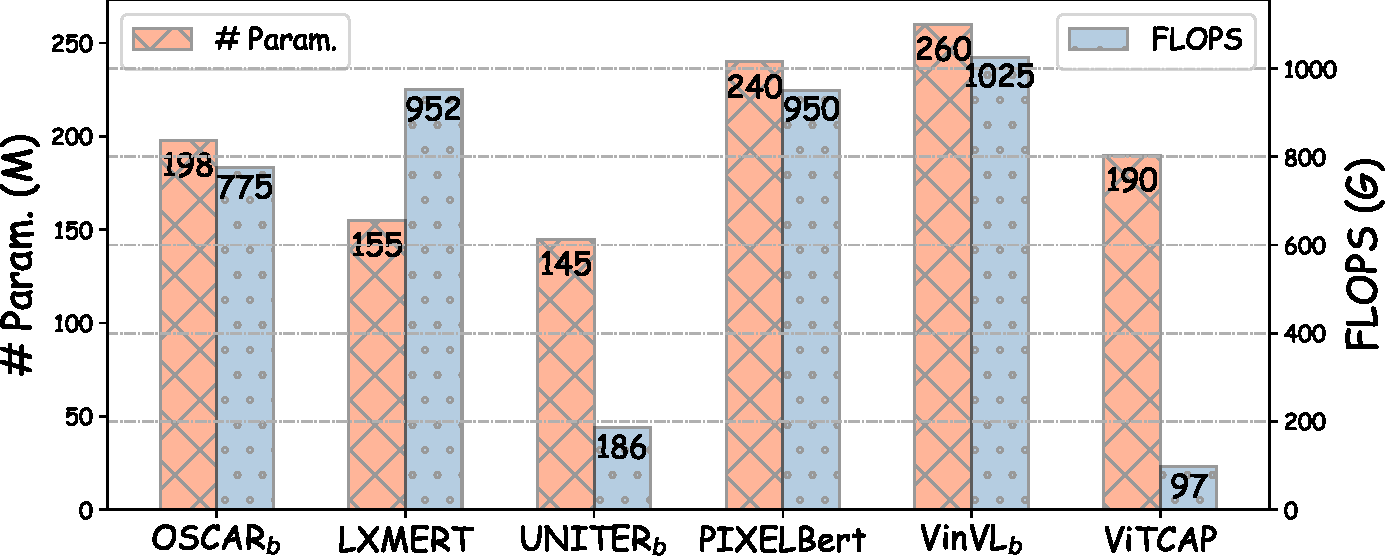
\includegraphics[width=.78\textwidth]{images/flops.pdf}
    \caption {\small Inference speed in FLOPs (in G), number of parameters (in M) of multiple VL models and \vitcapp\!\!.}
    \vspace{-1mm}
\label{fig:flops}
\end{figure}





% Table for semantic concepts
\begin{table}[t]
\centering
\renewcommand{\arraystretch}{1.15} 
\setlength\tabcolsep{8.5pt}
\caption[Adopting various sources of semantic concept leads to different performances.]{\small Adopting various sources of semantic concept leads to different performances. ``CAPTION'' represents the baseline extracting keywords from open-form captions; ``$^{\spadesuit}$'' is the baseline using all words in captions as target concepts; ``BUTD'' and ``VinVL'' represent using the object tags produced by the object detector from~\citep{anderson2018bottom} and~\citep{zhang2021multi} as target semantic concepts, respectively. ``VinVL $\rightarrow$ CAP.'' represents adopting detector tags~\citep{zhang2021multi} during first stage of concept classification and using caption extracted tags during the second stage.}
\scalebox{1.0}
{
\small
\begin{tabular}{p{42mm} | c c c c c }
\toprule
\multirow{2}{*}{\textbf{Concept Source}} & \multicolumn{4}{c}{{ \texttt{\textbf{\ \ \ \ \ COCO Captioning}}}}  \\ 
 & {B@4} & {\ \ M} & {\ \ R} & {\ \ C} & {\ \ S} \\
\hline
\cellcolor{black!3}\xmarkg  & \cellcolor{black!5}$33.9$ & $27.8$ & $56.4$ & \cellcolor{black!5}$114.8$ & $21.3$ \\
\cellcolor{red!3}BUTD & \cellcolor{black!15}$35.0$ & $28.2$ & $56.9$ & \cellcolor{gray!25}$117.4$& $21.3$ \\
\cellcolor{red!3}VinVL  & \cellcolor{black!25}$35.6$ & $28.6$ & $57.4$ & \cellcolor{gray!35}$119.7$ & $21.8$ \\
\cellcolor{red!3}CAPTION & \cellcolor{black!35}$35.6$ & $28.7$  & $57.6$ & \cellcolor{gray!35}$120.9$ & $21.8$ \\
\cellcolor{red!3}VinVL $\rightarrow$ CAP.$^{\spadesuit}$& \cellcolor{gray!35}$35.9$ & $28.6$  & $57.6$ & \cellcolor{gray!40}$121.3$ & $21.9$ \\
\cellcolor{red!3} CAPTION$^{\spadesuit}$ & \cellcolor{gray!45}$36.1$ & $28.8$ & $57.6$ & \cellcolor{gray!45}$122.2$ & $22.1$ \\ 
\bottomrule
\end{tabular}
}
\label{tab:tags}
\end{table}




\vspace{1mm}
\noindent \textbf{Semantic Concept Sources.} We study the effects of different semantic concept sources, \ie, from object detectors~\citep{anderson2018bottom,zhang2021multi}, captions-extacted concepts, and the combination of them. Table~\ref{tab:tags} lists the performances of \vitcap on the COCO caption dataset with various semantic concepts sources. 
Open-form captions are the most accessible source to directly obtain semantic concepts, although these descriptions can sometimes be noisy, inaccurate and incomplete. ``CAPTION'' in Table~\ref{tab:tags} is the result using nouns and adjectives parsed from captions using NLTK~\citep{loper2002nltk} toolkit as target concepts. This leads to an obvious improvement over the baseline (without CTN): CIDEr $120.9$ \vs $114.8$. 
We also attempt to leverage all tokens from the captions as concept targets in case of omitting essential words during parsing (see ``CAP.$^{\spadesuit}$''), which brings further incremental improvement and yield best result. Although using all tokens in the caption might inevitably introduce more noisy or irrelevant words, \eg, connection and stop words, it also broadens the semantic concepts vocabulary as some rare entities/attributes might be missed using just keywords. 
% Refer to the Appendix for more experimental setup details.

\begin{table}[t]
    \centering
    \renewcommand{\arraystretch}{1.2} .
    \caption[Comparisons of \vitcapp with or without knowledge distillation.]{\small Comparisons of \vitcapp with or without knowledge distillation, large-scale pre-training and with CTN. Performances are reported on COCO-caption Karpathy split optimized by cross-entropy loss. $_{+ \text{OD-TAG}}$ indicates the result using the detector produced off-the-shelf tags as~\citep{li2020oscar}. $_{+ \text{CTN-TOK}}$ is the result of \vitcapp using the initialization after first-stage concept classification. $_{\color{darkred}{\text{\textbf{KD}}}}$ and $_{\color{darkgreen}{\text{\textbf{PRE}}}}$ are results obtained with masked token classification distillation and pre-training at scale respectively.
    }    
    \scalebox{0.95}
    {\small
    \begin{tabular}{p{43.5mm} c c c c c }
    \toprule
    \\[-3.5ex]
   \multirow{2}{*}{\textbf{Methods}} & \multicolumn{4}{c}{{\texttt{\textbf{\ \ \ \ Cross-Entropy Loss}}}} \\
    & \multicolumn{1}{c}{B@4 } & M & R  & C     & \multicolumn{1}{c}{S}    \\	
    \hline
    \cellcolor{red!3}ViT/B&   \cellcolor{gray!5}$33.9$ & $27.8$ & $56.4$ &  \cellcolor{gray!5}$114.8$ & $21.3$ \\
    \cellcolor{red!3}ViT/B${\tiny  \scalebox{1.1}{+} \  \color{darkred}{\text{\textbf{KD}}}}$ &   \cellcolor{gray!20}$35.4$ & $28.5$ & $57.5$ & \cellcolor{gray!40}$120.0$ & $21.7$   \\
    \cellcolor{red!3}ViT/B${\tiny \scalebox{1.1}{+} \ \text{CTN-TAG}}$ &    \cellcolor{gray!15}$35.2$ &  $28.0$ & $57.0$ &	\cellcolor{gray!25}$117.1$ & $21.4$ \\
    \cellcolor{red!3}ViT/B${\tiny \scalebox{1.1}{+} \ \text{OD-TAG}}$ &    \cellcolor{gray!10}$34.3$ &  $28.2$ & $57.4$	& \cellcolor{gray!25}$117.4$ & $21.7$\\
    \cellcolor{red!3}ViTCAP${\tiny \scalebox{1.1}{+} \ \text{CTN-TOK}{\color{black}}}$ &    \cellcolor{gray!25}$36.1$ &  $28.8$ & $57.6$	& \cellcolor{gray!35}$122.2$ & $22.1$\\
    % ViTCAP${\tiny \scalebox{1.1}{+} \ \text{VC-TOK} \scalebox{1.1}{+} \ {\color{darkred}{\text{\textbf{KD}}}}  }$ \\
    \cellcolor{red!3}ViTCAP${\tiny \scalebox{1.1}{+} \ \text{CTN-TOK}  \scalebox{1.1}{+} \ {\color{ddarkgreen}{\text{\textbf{PRE}}}} \scalebox{1.1}{+} {\color{darkred}{\text{\textbf{KD}}}} }$ &  \cellcolor{gray!35}$36.3$ &  $29.3$ & $58.1$ & \cellcolor{gray!45}$125.2$ & $22.6$   \\
    \bottomrule
    \end{tabular}
    }
  \label{tab:ablation}
\end{table}
% We also resort to different object detectors to acquire high-quality semantic concepts, \ie, a ResNet$_{101}$ base Faster-RCNN~\citep{anderson2018bottom} that has been pre-trained on Visual-Genome dataset~\citep{krishna2017visual} (denoted as BUTD), and a ResNext$_{152}$ based modified Faster-RCNN detector with broader categories of the visual attribute as detection targets (denoted as VinVL). Although these detector-produced image-level tags are rather accurate with less noise, they require a pre-defined categorical dictionary with a fixed set of vocabulary. We first extract these tags as off-the-shelf annotations for the classification task on a ViT/B model and apply it as the initialization of \vitcap for captioning training. Note that we conduct and compare all these ablations without pre-training. We showcase some qualitative examples with the produced image-level semantic concepts in the Appendix.
We then experiment with using the detectors in~\citep{zhang2021multi} and~\citep{anderson2018bottom} to produce image-level tags as target concepts. We observe that using the detector of VinVL yields better performances than BUTD, \ie, $119.7$ \vs $117.4$ CIDEr scores. This is mainly because of the more diverse collection of semantic concepts involved in~\citep{zhang2021multi} than BUTD~\citep{anderson2018bottom}. 
% including $1,848$ object labels and $524$ attribute labels involved in detection training. 
% Noticeably, direct learning from the caption-extracted keywords leads to better results and by using all tokens as target concepts (denoted CAPTION$^{\spadesuit}$). 
The second last row is the experiment where the model is firstly trained using VinVL tags on large scale dataset (in the first stage), and then using the caption tokens during the second stage of captioning. This indicates that, when no captions are attainable, it is also viable to leverage detector-produced tags to improve the performance.
% This suggests that the extracted concepts enrich the vocabulary and therefore produce tokens with more semantics for the captioning task. 
% This also largely alleviates the challenge where the semantic concepts in the target domain are in different forms \textit{w.r.t.} the source domain descriptions. For example, synonym, cognate and conjugate words or various tenses.


\begin{table}[t!]
\centering
\renewcommand{\arraystretch}{1.05} % Default value: 1
\caption[Performances of \vitcapp model on Conceptual Captions (Google-CC 3M dev-split)~\citep{sharma2018conceptual} benchmark.]{\small
Performances of \vitcapp model on Conceptual Captions (Google-CC 3M dev-split)~\citep{sharma2018conceptual} benchmark. We compare with the baseline methods FRCNN~\citep{changpinyo2019decoupled}, Ultra~\citep{changpinyo2019decoupled} and~\citep{changpinyo2021conceptual}. The ViLT-CAP$^{\color{black}{\spadesuit}}$ and VinVL represent our reproduced results with pre-trained checkpoint from~\citep{kim2021vilt} and~\citep{zhang2021multi}.
}
\scalebox{0.99}
{ 
\small
\begin{tabular}{l|c}
\toprule
\multirow{2}{*}{\textbf{Methods}}  & \multicolumn{1}{c}{{ \texttt{\textbf{CC-3M dev}}}}  \\ 
& {CIDEr} \\
\hline 
   \cellcolor{red!3}FRCNN & $89.2$ \\
   \cellcolor{red!3}Ultra & $93.7$ \\ 
   \cellcolor{red!3}VILT-CAP$^{\color{black}{\spadesuit}}$ & $83.8$\\ 
   \cellcolor{red!3}VinVL$^{\color{black}{\spadesuit}}$ & $103.4$ \\ 
   \cellcolor{red!3}CC-$3$M & $100.9$ \\
   \cellcolor{red!3}CC-$12$M & $105.4$ \\ 
   \hline
   \cellcolor{blue!3}ViTCAP  &  $\textbf{108.6}_\text{\color{darkgreen}\textbf{ +3.2}}$ \\
\bottomrule
\end{tabular}
}
\label{tab:googlecc}
\end{table}


\begin{table}[t!]
    \centering
    \setlength{\tabcolsep}{6pt} % Default value: 6pt
    \renewcommand{\arraystretch}{1.05} % Default value: 1
    \caption [Performances of \vitcapp in nocaps validation split.]{\small Performances of \vitcapp in nocaps validation split. We compare our \vitcapp with previous state-of-the-art models at \textbf{``in-domain''}, \textbf{``near-domain''} and \textbf{``out-of-domain''}. Results are reported with constrained beam search (CBS) decoding~\citep{anderson2016guided}.}    
    \scalebox{0.88}
    {
     \small
    \begin{tabular}{l|cc|cc|cc|cc}
    \toprule
    & \multicolumn{8}{c}{\texttt{\textbf{nocaps validation set}}} \\
    \cline{2-9} 
    \multicolumn{1}{l|}{\textbf{Methods}} & \multicolumn{2}{c|}{\textbf{in-domain}} & \multicolumn{2}{c|}{\textbf{near-domain}} &  \multicolumn{2}{c|}{\textbf{out-of-domain}} & \multicolumn{2}{c}{\textbf{overall}}\\ 
     & C & S & C &  S  & C & S & C & S \\ 
    \hline 
    \transparent{0.4}Human & \transparent{0.4}84.4 & \transparent{0.4}\textbf{14.3} & \transparent{0.4}85.0 & \transparent{0.4}\textbf{14.3} & \transparent{0.4}\textbf{95.7} & \transparent{0.4}\textbf{14.0} & \transparent{0.4}87.1 & \transparent{0.4}\textbf{14.2} \\
    \hline
    \cellcolor{red!3}UpDown & $78.1$ & $11.6$ & $57.7$ & $10.3$ & $31.3$ & $8.3$ & $55.3$ & $10.1$ \\
    \cellcolor{red!3}UpDown + CBS  & $80.0$ & $12.0$ & $73.6$ & $11.3$ & $66.4$ & $9.7$ & $73.1$ & $11.1$ \\
    \cellcolor{red!3}UpDown + ELMO + CBS  & $80.0$ & $12.0$ & $73.6$ & $11.3$ & $66.4$ & $9.7$ & $73.1$ & $11.1$ \\
    % UpDown~\citep{agrawal2019nocaps} + ELMo + CBS & $79.3$ & $12.4$ & $73.8$ & $11.4$ & $71.7$ & $9.9$ & $74.3$ & $11.2$ \\ 
    % UpDown~\citep{agrawal2019nocaps}& $79.3$ & $12.4$ & $73.8$ & $11.4$ & $71.7$ & $9.9$ & $74.3$ & $11.2$ \\ 
    % \hline
    % Oscar$_L$~\citep{li2020oscar} & 79.9 & 12.4 & 68.2 & 11.8 & 45.1 & 9.4 & 65.2 & 11.4 \\
    \cellcolor{red!3}OSCAR & $79.6$ & $12.3$ & $66.1$ & $11.5$ & $45.3$ & $9.7$ & $63.8$ & $11.2$ \\
    \cellcolor{red!3}OSCAR + CBS & $83.4$ & $12.0$ & $81.6$ & $12.0$ & $77.6$ & $10.6$ & $81.1$ & $11.7$ \\
    % Oscar$_L$ + CBS & 78.8 & 12.2 & 78.9 & 12.1 & 77.4 & 10.5 & 78.6 & 11.8 \\
    % OSCAR$_\text{L}$~\citep{li2020oscar}& $85.4$ & $11.9$ & $84.0$ & $11.7$ & $80.3$ & $10.0$ & $83.4$ & $11.4$ \\ 
    % \hline
    % VIVO~\citep{hu2020vivo} & 88.8 & 12.9 & 83.2 & {12.6} & 71.1 & 10.6 & 81.5 & 12.2 \\
    % VIVO + CBS & 90.4 & {13.0} & 84.9 & 12.5 & 83.0 & 10.7 & 85.3 & 12.2 \\
    \cellcolor{red!3}VIVO  & $90.4$ & $13.0$ & $84.9$ & $12.5$ & $83.0$ & $10.7$ & $85.3$ & $12.2$ \\
    \cellcolor{red!3}VIVO + CBS & $92.2$ & $12.9$ & $87.8$ & $12.6$ & $87.5$ & $11.5$ & $88.3$ & $12.4$ \\
    \hline
    \cellcolor{blue!3}\vitcap  & $\textbf{99.3}$ & $13.2$ & $90.4$ & $12.9$ & $78.1$ & $11.9$ & $89.2$ & $12.7$ \\
    \cellcolor{blue!3}\vitcap + CBS & $98.7$ & $13.3$ & $\textbf{92.3}$ & $13.3$ & ${95.4}$ & ${12.7}$ & $\textbf{93.8}$ & $13.0$ \\ [-6pt]
     $_{\color{black}\Delta}$ & $_\text{\color{darkgreen}\textbf{+6.5}}$ & $_\text{\color{darkgreen}\textbf{+0.4}}$ & $_\text{\color{darkgreen}\textbf{+4.5}}$ & $_\text{\color{darkgreen}\textbf{+0.7}}$ & $_\text{\color{darkgreen}\textbf{+7.9}}$ & $_\text{\color{darkgreen}\textbf{+1.2}}$ &
     $_\text{\color{darkgreen}\textbf{+5.5}}$ &
     $_\text{\color{darkgreen}\textbf{+0.6}}$ \\
    \bottomrule
    \end{tabular}
    }
    \label{tab:arch}
\end{table}

% architectural variations and Google CC result
% \begin{table*}[t!]
% 	\begin{minipage}{0.28\linewidth}
%     \centering
%     \renewcommand{\arraystretch}{1.05} % Default value: 1
%     \scalebox{0.72}
%     { 
%     \small
%     \begin{tabular}{l|c}
%     \toprule
%     \multirow{2}{*}{\textbf{Methods}}  & \multicolumn{1}{c}{{ \texttt{\textbf{CC-3M dev}}}}  \\ 
%     & {CIDEr} \\
%     \hline 
%       \cellcolor{red!3}FRCNN & $89.2$ \\
%       \cellcolor{red!3}Ultra & $93.7$ \\ 
%       \cellcolor{red!3}VILT-CAP$^{\color{black}{\spadesuit}}$ & $83.8$\\ 
%       \cellcolor{red!3}VinVL$^{\color{black}{\spadesuit}}$ & $103.4$ \\ 
%       \cellcolor{red!3}CC-$3$M & $100.9$ \\
%       \cellcolor{red!3}CC-$12$M & $105.4$ \\ 
%       \hline
%       \cellcolor{blue!3}ViTCAP  &  $\textbf{108.6}_\text{\color{darkgreen}\textbf{ +3.2}}$ \\
%     \bottomrule
%     \end{tabular}
%     }
%     % \vspace{-2mm}
%     \caption[Performances of \vitcapp model on Conceptual Captions (Google-CC 3M dev-split)~\citep{sharma2018conceptual} benchmark.]{\small
%     Performances of \vitcapp model on Conceptual Captions (Google-CC 3M dev-split)~\citep{sharma2018conceptual} benchmark. We compare with the baseline methods FRCNN~\citep{changpinyo2019decoupled}, Ultra~\citep{changpinyo2019decoupled} and~\citep{changpinyo2021conceptual}. The ViLT-CAP$^{\color{black}{\spadesuit}}$ and VinVL represent our reproduced results with pre-trained checkpoint from~\citep{kim2021vilt} and~\citep{zhang2021multi}.
%     }
%     \label{tab:googlecc}
% 	\end{minipage} \hfill
% 	\begin{minipage}{0.64\linewidth}
%     \centering
%     \setlength{\tabcolsep}{4pt} % Default value: 6pt
%     \renewcommand{\arraystretch}{1.05} % Default value: 1
%     \scalebox{0.58}
%     {
%      \small
%     \begin{tabular}{l|cc|cc|cc|cc}
%     \toprule
%     & \multicolumn{8}{c}{\texttt{\textbf{nocaps validation set}}} \\
%     \cline{2-9} 
%     \multicolumn{1}{l|}{\textbf{Methods}} & \multicolumn{2}{c|}{\textbf{in-domain}} & \multicolumn{2}{c|}{\textbf{near-domain}} &  \multicolumn{2}{c|}{\textbf{out-of-domain}} & \multicolumn{2}{c}{\textbf{overall}}\\ 
%      & C & S & C &  S  & C & S & C & S \\ 
%     \hline 
%     \transparent{0.4}Human & \transparent{0.4}84.4 & \transparent{0.4}\textbf{14.3} & \transparent{0.4}85.0 & \transparent{0.4}\textbf{14.3} & \transparent{0.4}\textbf{95.7} & \transparent{0.4}\textbf{14.0} & \transparent{0.4}87.1 & \transparent{0.4}\textbf{14.2} \\
%     \hline
%     \cellcolor{red!3}UpDown & $78.1$ & $11.6$ & $57.7$ & $10.3$ & $31.3$ & $8.3$ & $55.3$ & $10.1$ \\
%     \cellcolor{red!3}UpDown + CBS  & $80.0$ & $12.0$ & $73.6$ & $11.3$ & $66.4$ & $9.7$ & $73.1$ & $11.1$ \\
%     \cellcolor{red!3}UpDown + ELMO + CBS  & $80.0$ & $12.0$ & $73.6$ & $11.3$ & $66.4$ & $9.7$ & $73.1$ & $11.1$ \\
%     % UpDown~\citep{agrawal2019nocaps} + ELMo + CBS & $79.3$ & $12.4$ & $73.8$ & $11.4$ & $71.7$ & $9.9$ & $74.3$ & $11.2$ \\ 
%     % UpDown~\citep{agrawal2019nocaps}& $79.3$ & $12.4$ & $73.8$ & $11.4$ & $71.7$ & $9.9$ & $74.3$ & $11.2$ \\ 
%     % \hline
%     % Oscar$_L$~\citep{li2020oscar} & 79.9 & 12.4 & 68.2 & 11.8 & 45.1 & 9.4 & 65.2 & 11.4 \\
%     \cellcolor{red!3}OSCAR & $79.6$ & $12.3$ & $66.1$ & $11.5$ & $45.3$ & $9.7$ & $63.8$ & $11.2$ \\
%     \cellcolor{red!3}OSCAR + CBS & $83.4$ & $12.0$ & $81.6$ & $12.0$ & $77.6$ & $10.6$ & $81.1$ & $11.7$ \\
%     % Oscar$_L$ + CBS & 78.8 & 12.2 & 78.9 & 12.1 & 77.4 & 10.5 & 78.6 & 11.8 \\
%     % OSCAR$_\text{L}$~\citep{li2020oscar}& $85.4$ & $11.9$ & $84.0$ & $11.7$ & $80.3$ & $10.0$ & $83.4$ & $11.4$ \\ 
%     % \hline
%     % VIVO~\citep{hu2020vivo} & 88.8 & 12.9 & 83.2 & {12.6} & 71.1 & 10.6 & 81.5 & 12.2 \\
%     % VIVO + CBS & 90.4 & {13.0} & 84.9 & 12.5 & 83.0 & 10.7 & 85.3 & 12.2 \\
%     \cellcolor{red!3}VIVO  & $90.4$ & $13.0$ & $84.9$ & $12.5$ & $83.0$ & $10.7$ & $85.3$ & $12.2$ \\
%     \cellcolor{red!3}VIVO + CBS & $92.2$ & $12.9$ & $87.8$ & $12.6$ & $87.5$ & $11.5$ & $88.3$ & $12.4$ \\
%     \hline
%     \cellcolor{blue!3}\vitcap  & $\textbf{99.3}$ & $13.2$ & $90.4$ & $12.9$ & $78.1$ & $11.9$ & $89.2$ & $12.7$ \\
%     \cellcolor{blue!3}\vitcap + CBS & $98.7$ & $13.3$ & $\textbf{92.3}$ & $13.3$ & ${95.4}$ & ${12.7}$ & $\textbf{93.8}$ & $13.0$ \\ [-6pt]
%      $_{\color{black}\Delta}$ & $_\text{\color{darkgreen}\textbf{+6.5}}$ & $_\text{\color{darkgreen}\textbf{+0.4}}$ & $_\text{\color{darkgreen}\textbf{+4.5}}$ & $_\text{\color{darkgreen}\textbf{+0.7}}$ & $_\text{\color{darkgreen}\textbf{+7.9}}$ & $_\text{\color{darkgreen}\textbf{+1.2}}$ &
%      $_\text{\color{darkgreen}\textbf{+5.5}}$ &
%      $_\text{\color{darkgreen}\textbf{+0.6}}$ \\
%     \bottomrule
%     \end{tabular}
%     }
%     \vspace{1mm}
%     \caption [Performances of \vitcapp in nocaps validation split.]{\small Performances of \vitcapp in nocaps validation split. We compare our \vitcapp with previous state-of-the-art models at \textbf{``in-domain''}, \textbf{``near-domain''} and \textbf{``out-of-domain''}. Results are reported with constrained beam search (CBS) decoding~\citep{anderson2016guided}.}
%     \label{tab:arch}
% 	\end{minipage} \ \ \
% 	\vspace{-4mm}
% \end{table*}


\noindent \textbf{Effect of Different Modules.} \label{sec:module} In Table~\ref{tab:ablation}, we show in details the independent performance gains from each design, \textit{viz.}, with or without concept tokens, masked token distillation loss, pre-training and the combinations of them. 
We report the result of the baseline model 
% is built upon the ViT base architecture using patch size $16\times16$ (ViT/B-16), 
which reaches CIDEr scores $114.8$ on COCO caption dataset. 
With the aim of isolating the performance gain from concept tokens, we first decode the image-level semantic concepts and store them as offline tags for the captioning task. We then follow~\citep{li2020oscar} to tokenize them and concatenate the tag embedding with visual features for captioning task. This allows us to directly compare the effect of CTN-produced concepts with detector tags without the concept classification initialization.
Adopting the explicit tags predicted by the CTN leads to obvious improvements: $2.3$ higher CIDEr and $1.3$ higher BLEU@$4$ scores, reaching similar results with that using VinVL's detector tags directly (see ViT/B$_\text{+OD-TAG}$): $117.4$ \vs $117.1$ CIDEr scores. This proves that our generated semantic concepts play a significant role in the captioning task and have a similar effect as the VinVL's detector tags. Next, we apply the pre-trained weights after the concept classification to initialize the \vitcap for the captioning task, and find further improvement (see ViTCAP${_\text{+CTN-TOK}}$). 
% : $36.1$ BLEU@$4$ and $122.2$ CIDEr scores
This proves that both the predicted concept tokens and the concept classification training are beneficial captioning tasks. 
For the knowledge distillation experiment, we use the VinVL-base~\citep{zhang2021multi} optimized on COCO-caption dataset as the Teacher and keep it frozen during distillation.
The application of KD on masked token prediction (ViT/B${_\text{+\color{darkred}{\textbf{KD}}}}$) is also evidently helpful: there is an over $5.0$ CIDEr scores improvement over the baseline. Note that the KD objective is only applied in the downstream for the \vitcap baseline after VLP for fair comparison with previous works. 
% The later experiment also verifies that the application of KD is complementary with concept tokens. 
Finally, by pre-training the \vitcap with large scale VL corpus continuously contributes to the results.




% \vspace{1mm}
\noindent \textbf{Performances on other Benchmarks.}
\label{sec:otherdata} To evaluate the generalizability of ViTCAP, we continue to expand the testbeds to other challenging captioning benchmarks, \ie, Google-CC~\citep{sharma2018conceptual} and nocaps~\citep{agrawal2019nocaps} datasets. For the Google-CC dataset, we train the \vitcap on the training split, which consists of ${\sim}3.3$M image-caption pairs, and test it on the dev split. We follow the same training protocols as previously mentioned and optimize the \vitcap for $120$ epochs.  Following previous works, we evaluate the performances using the CIDEr metric and Table~\ref{tab:googlecc} shows the results of \vitcap compared with previous captioning models. In particular, \vitcap achieves the state-of-the-art results CIDEr $108.6$ scores (without the knowledge distillation), surpassing all detector-based captioning models. CC-$12$M is the model trained with $12$M image-caption pairs~\citep{changpinyo2021conceptual}. Again, when evaluating on nocaps dataset, \vitcap  shows promissing results across all in-domain, near-domain, and out-of-domain splits. For example, \vitcap achieves $98.7$ and $93.8$ CIDEr scores on in/out-domain splits, $6.5$ and $5.5$ higher than the VIVO~\citep{hu2020vivo}, which exploits OpenImage~\citep{kuznetsova2020open} dataset to learn semantic concepts for captioning task. 
The great generalization ability of \vitcap can be partly ascribed to its ability to recognize expansive semantic concepts extracted from the open-form captions. Compared to predicting the pre-defined tags as in the detector, the usage of caption extracted concepts largely expands the concept vocabulary. This provides the \vitcap with robust and broad concept tokens, which is essential for the images with novel concepts. 



\begin{figure}[t!]
%  \vspace{-3mm}
  \begin{center}
  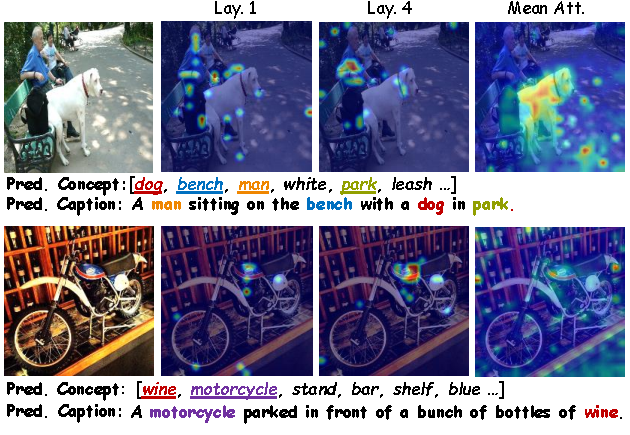
\includegraphics[width=.86\textwidth]{images/main_qualitative.pdf}
  \end{center}
  \vspace{-6mm}
    \caption[Visualization of the attention maps from \vitcapp and its produced concepts\&captions.]{\small Visualization of the attention maps from \vitcapp and its produced concepts\&captions. ``\rule{6mm}{0.15mm}'' refers to the concepts appear in captions. Best viewed in colors.
    }
    \vspace{-4mm}
  \label{fig:qualitative}
\end{figure}



\vspace{1mm}
\noindent \textbf{Qualitative Examples.} We show visualization examples of the attention maps from \vitcap in Figure~\ref{fig:qualitative} together with their generated concepts\&captions. Interestingly, we observe obvious correlations between the attended regions across different layers and predicted concepts. For example, ``{\color{black} \texttt{\textbf{dog}}}'' is notably highlighted according to the mean-averaged attention maps, yet the ``{\color{black} \texttt{\textbf{man}}}'' is more attended in shallower transformer blocks. We conjecture that instead of relying on an object detector to glean object locations, training the detector-free VL model properly via image-text supervisions might potentially lead to a strong grounding model as a promising future endeavor. 



\begin{figure}[t!]
    \centering
    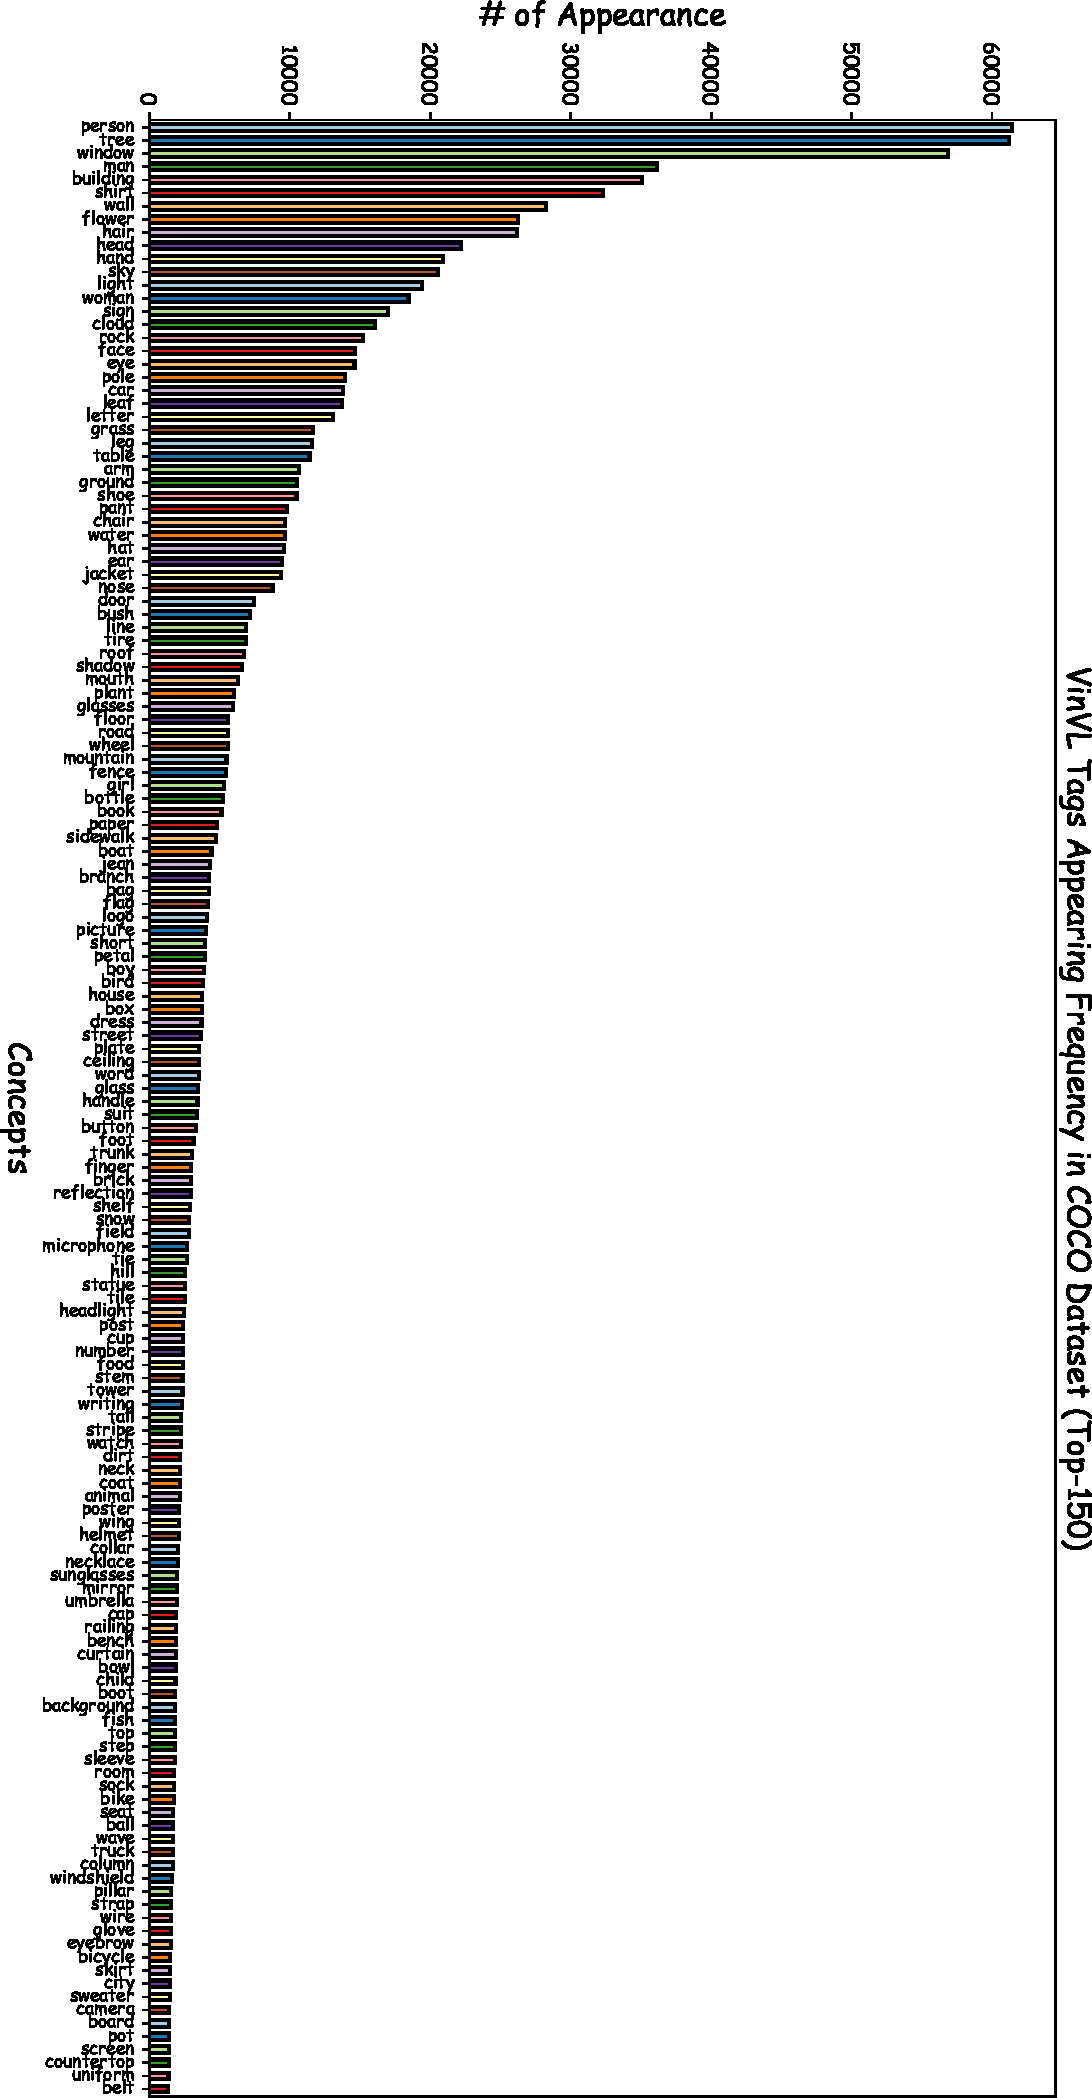
\includegraphics[width=.7\linewidth]{images/stats_rotated.pdf}
    \caption[Top-$150$ most frequently appeared semantic concepts produced by VinVL's object detector.]{Top-$150$ most frequently appeared semantic concepts produced by VinVL's object detector. The produced tags are severely long-tail distributed and certain concepts dominates across all samples. This arises the necessity to apply focal loss as countermeasure. }
    \label{fig:stats}
\end{figure}



  
 
\begin{table}[t!]
\begin{center}
\caption{Statistics of the VL pre-training datasets. }
\begin{tabular}{c@{\hspace{3pt}}|c@{\hspace{3pt}}|c|c|c@{\hspace{3pt}}}
\toprule
Source & VG & COCO & CC& SBU\\
\midrule
Image & 108K & 113K & 3.1M & 875K  \\
Text & 5.4M & 567K & 3.1M & 875K  \\
\bottomrule
\end{tabular}
\end{center}
\label{tab:vlcorpus}
\end{table}


\subsubsection{Pre-training VL Corpus}
As previous works in~\citep{zhang2021multi}, we carry out the pre-training of ViTCAP on the aggregation of several common datasets, which include COCO~\citep{lin2014microsoft}, Conceptual Caption~\citep{changpinyo2021conceptual}, SBU Captions~\citep{ordonez2011im2text}, and Visual Genome~\citep{krishna2017visual}. We have the detailed statistics of the aggregated datasets in the above Table. In total, we use $4.2$ millions images and $9.9$M captions for the pre-training. Following~\citep{lu202012}, we de-duplicate images exist in both pre-training corpus and COCO Karpathy testing splits for fair comparisons.



\subsubsection{Ablative Studies}
This section further presents additional ablative studies about ViTCAP, which includes: some examples and basic statistics about semantic concepts, effect of differnet concept sources, 
results of different concept classification losses, different other training strategies.



\vspace{1mm}
\noindent\textbf{Examples and Stats of Concepts.}
In practice, we experiment with utilizing semantic concepts gleaned from 1). open-form image captions by language parsing (or simple as using all tokens as classification ground-truth) or 2).  an object detector. 

As previously mentioned, we notice that the concepts from both sides are all severely long-tailed distributed (an example of the detector-produced concept distribution is shown in Figure~\ref{fig:stats}). Notably, certain concepts appear more frequently across the whole COCO training split, \eg, ``\texttt{person}'', ``\texttt{tree}'', ``\texttt{window}'' obviously exist far more frequent than the remaining.  We also resort to different object detectors to acquire high-quality semantic concepts, \ie, a ResNet$_{101}$ base Faster-RCNN~\citep{anderson2018bottom} that has been pre-trained on Visual-Genome dataset~\citep{krishna2017visual} (denoted as BUTD), and a ResNext$_{152}$ based modified Faster-RCNN detector with broader categories of the visual attribute as detection targets (denoted as VinVL). These detector-produced image-level tags are actually accurate with less noise as in captions, but they also require the pre-defined categorical dictionary with fixed set of concepts. This largely limits the scope of their applications.

\vspace{1mm}
\noindent\textbf{More About Concept Sources.}
Open-form captions are the most idea source to obtain semantic concepts as they naturally carry abundant semantic concepts with no vocabulary limitation. Notwithstanding that most of these descriptions can be noisy, inaccurate and incomplete. In practice, we leverage different ways to extract the concepts from them by 1) using the NLTK~\citep{loper2002nltk} toolkit and parse out only the nouns and adjectives as the semantic concepts for the classification task (see ``CAPTION'' baseline in main paper); 2) we also simply attempt to leverage all tokens from the captions as concept targets in case of omitting essential words during parsing (see ``$^{\spadesuit}$'' in main paper).
We first extract these tags as ``\textit{off-the-shelf}'' annotations for the concept classification task and then apply the initialization of VitCAP after first stage training for the joint captioning training. Note that we conduct and compare all these ablations without VL pre-training. It is beneficial to further adopt the concept classification loss during the joint training, as the semantic concepts in the COCO-caption dataset vary with the concept classification dataset. Also, captions in these two domains might vary from the aspect of textual styles: for example, length of captions, the use of synonym, cognate and conjugate words or various tenses.



\begin{table}[h]
\centering
\setlength{\tabcolsep}{4pt} % Default value: 6pt
\renewcommand{\arraystretch}{1.15} % Default value: 1
\caption{\small Performances of ViTCAP using focal loss, binary classification loss as concept classification training target. 
}
% \vspace{-2mm}
\scalebox{0.99}{
 \small
\begin{tabular}{l|c|ccccc}
\toprule
 & \multicolumn{5}{c}{{ \texttt{\textbf{COCO Captioning}}}}  \\ 
& EPOCH & {B@4} & {M} & {R} & {C} & {S} \\
\hline 
%  {\transparent{0.4} Baseline$_{32\times32}$} & {\transparent{0.4} -} & {\transparent{0.4} $33.9$} &
  {\transparent{0.4} Baseline} & {\transparent{0.4} -} & {\transparent{0.4} $33.9$} &
  {\transparent{0.4} $27.8$} &  {\transparent{0.4} $56.4$} & {\transparent{0.4} $114.8$} &  {\transparent{0.4} $21.3$} \\
 {\transparent{0.4} VinVL-Tag} & {\transparent{0.4} -} & {\transparent{0.4} $35.4$} & {\transparent{0.4} $28.1$} &  {\transparent{0.4} $57.2$} & {\transparent{0.4} $117.7$} &  {\transparent{0.4} $21.3$} \\
\hline
% BCE$_\text{Tag}$  & $10$ & \\ 
BCE$_\text{Tag}$  & $10$ & $33.9$ & $27.9$ & $56.5$ & $115.0$ & $21.4$\\ 
FOCAL$_\text{Tag}$ & $10$ & $35.2$ & $28.0$ & $57.0$ & $117.1$ & $21.4$\\ 
FOCAL$_\text{Tag+Init}$ & $10$ & $36.0$ & $28.4$ & $57.5$ & $120.5$ & $22.0$\\ 
FOCAL$_\text{Init}$ & $10$ & $35.0$ & $28.2$ & $57.1$ & $118.0$ & $21.6$\\ 
FOCAL$_\text{Tag+Init}$ & $40$ & $35.9$ & $28.4$ & $57.6$ & $121.1$ & $22.1$ \\ 
\bottomrule
\end{tabular}
}
\label{tab:losses}
\end{table} 

\vspace{1mm}
\noindent\textbf{Concept Classification Training.}
We now study the effect of different losses for the concept classification task, namely binary cross-entropy loss and the focal loss and the effect of the initialization after the classification training. 
The extremely imbalanced sample distribution usually lead to sub-optimal classification performances, as also studied in previous works like face recognition~\citep{zhang2017range,ma2020learning} and object detection~\citep{li2020overcoming, ouyang2016factors}, etc. As countermeasures, there exist works designing advanced losses~\citep{lin2017focal,zhang2017range} re-weighting different samples. In Table~\ref{tab:losses}, we list the performances of ViTCAP using different losses. In specific, the top-two rows are the baseline results 1). Baseline: vanilla Encoder-Decoder architecture without CTN branch, and 2). Encoder-Decoder architecture using VinVL's OD tags as~\citep{li2020oscar}. ``$_\text{Tag}$'' denotes the results are reported using concepts as the offline tags without concept classification \& its initialization. We observe that by applying the BCE loss trained offline concepts as offline tags, the results are only incrementally improved over the baseline, and it still shows a great performance gap \textit{w.r.t.} the VinVL's tag. Notably, using focal loss obviously improves the quality of produced concepts, reaching $117.1$ CIDEr scores. To this end, we apply the concept classification pre-trained initialization, and this
further improves the performances to a great extent. It is discernible that the experiment ``$_\text{Init}$'' gives worse result than the ``$_\text{Tag+Init}$''. This validates that both the concept classification task and the predicted concepts are helpful for the captioning task. Results show that they are complementary to each other.


\begin{table}[h]
\centering
\setlength{\tabcolsep}{4pt} % Default value: 6pt
\renewcommand{\arraystretch}{1.15} % Default value: 1
\caption{\small Performances of VitCAP using different strategies for concept tokenization. 
}
% \vspace{-2mm}
\scalebox{0.99}{
 \small
\begin{tabular}{l|ccccc}
\toprule
\multirow{2}{*}{Tokenization} & \multicolumn{5}{c}{{ \texttt{\textbf{COCO Captioning}}}}  \\ 
 & {B@4} & {M} & {R} & {C} & {S} \\
\hline 
Caption Tokenizer & $35.5$ & $28.5$ & $57.5$ & $119.7$ & $21.8$ \\ 
Classifier Tokenizer & $35.6$ & $28.4$ & $57.4$ & $119.8$ & $21.8$ \\ 
Independent Tokenizer & $35.9$ & $28.5$ & $57.6$ & $120.1$ & $21.9$ \\ 
\bottomrule
\end{tabular}
}
\label{tab:tokenizer}
\end{table} 

\noindent\textbf{Representing Concepts as Tokens.} There are multiple ways to encode the predicted concepts as continuous embedding for decoding stage. We study three different ways of encoding and present the results in Table~\ref{tab:tokenizer}, namely, 1). use the tokenizer for captioning, 2). use the concept classifier's tokenizer (in concept classification, we simply use the BERT tokenizer to encode the semantic concepts), 3). use an independent and untrained tokenizer. Though in practice, all three tokenizers are implemented based on the BERT tokenizer~\citep{devlin2018bert}, the embeddings from the three are entirely different. From the results, we observe fairly negligible performance gap: using independent tokenizer only yields $0.4$ higher CIDEr score. Though adopting an independent tokenizer yields the best result, it introduces additional parameters and thus we choose to share the tokenizer for captioning instead. 


% \section{More Details about Training\&Evaluation}


\begin{table}[h]
\centering
\setlength{\tabcolsep}{4pt} % Default value: 6pt
\renewcommand{\arraystretch}{1.15} % Default value: 1
\caption{\small Performances of ViTCAP using either ground-truth concepts for captioning, the concept network predicted concept tokens, or the mixed of them during training. 
}
% \vspace{-2mm}
\scalebox{0.99}{
 \small
\begin{tabular}{l|ccccc}
\toprule
\multirow{2}{*}{\textbf{}} & \multicolumn{5}{c}{{ \texttt{\textbf{COCO Captioning}}}}  \\ 
& {B@4} & {M} & {R} & {C} & {S} \\
\hline 
GT Concepts & $35.5$ & $28.4$ & $57.3$ & $119.1$ & $21.7$ \\ 
GT + PRED. Concepts & $35.2$ & $28.5$ & $57.3$ & $119.2$ & $21.8$\\ 
PRED. Concepts & $36.1$ & $28.6$ & $57.6$ & $120.6$ & $21.7$\\ 
\bottomrule
\end{tabular}
}
\label{tab:concept}
\end{table} 

We experiment with different ways to train with the concept tokens. In Table~\ref{tab:concept}, we list results of training using GT semantic concepts encoded as tokens, GT concepts mixed with predicted concepts, and fully predicted concepts.

\begin{figure*}[h!]
  \begin{center}
    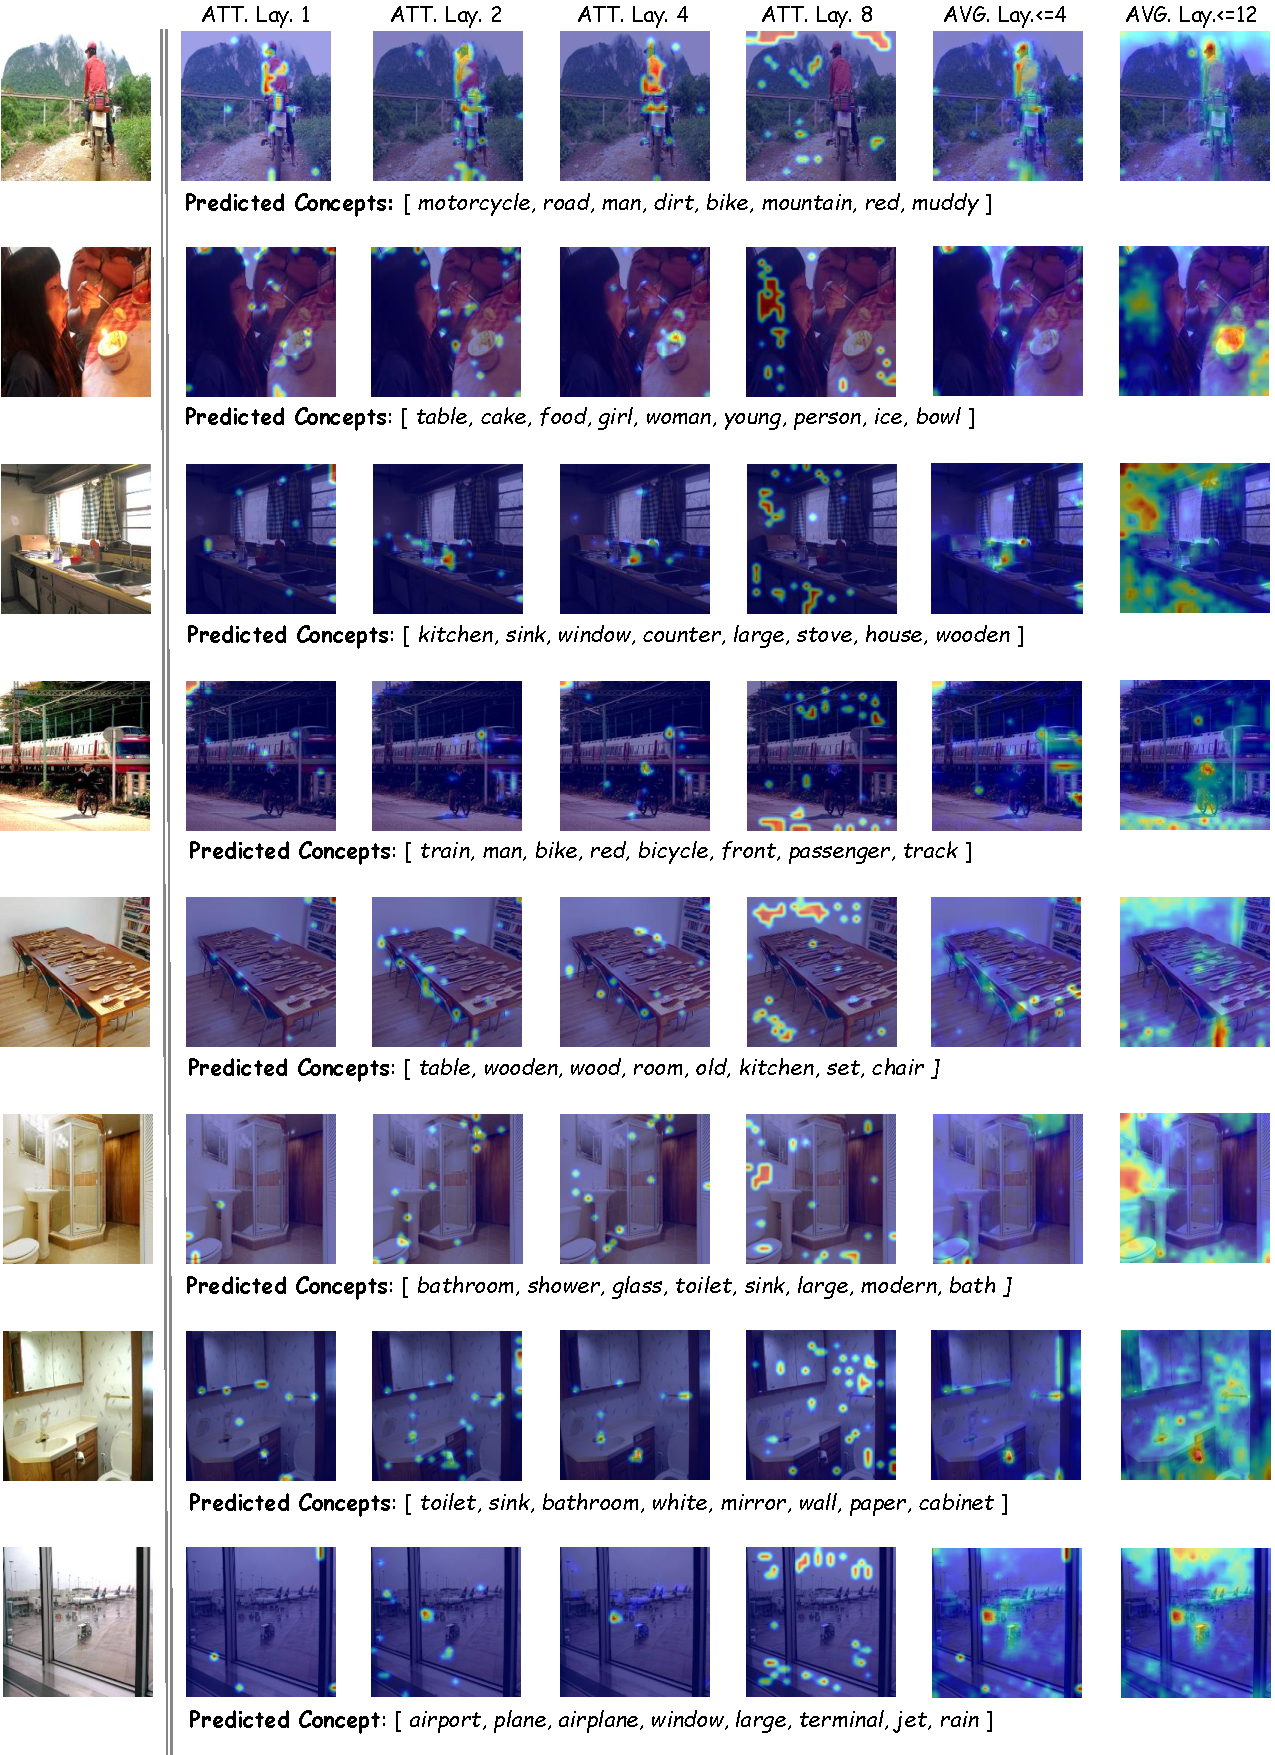
\includegraphics[width=0.9\textwidth]{./images/vitcap_qualitative.pdf}
    \vspace{-6mm}
  \end{center}
    \caption[ViTCAP produced class-agnostic attention maps and their associated semantic concepts of random images from COCO caption dataset. ]{\small ViTCAP produced class-agnostic attention maps and their associated semantic concepts of random images from COCO caption dataset. We exhibit attention maps of $1$, $2$, $4$, $8$th transformer blocks of ViTCAP and the mean-average attention maps of first $4$ and the entire $12$ transformer blocks (last two columns).
    }
  \label{fig:qualitative}
\end{figure*}

We find that by using the predicted concepts for training lead to optimal results. This is mostly because that the pre-trained CTN can already produce reasonable concepts at the captioning fine-tuning stage. 


\begin{table}[h]
\centering
\setlength{\tabcolsep}{6pt} % Default value: 6pt
\renewcommand{\arraystretch}{1.15} % Default value: 1
% \vspace{-2mm}
\caption[We compare different instantiations of ViTCAP with architectural variations of ViT based captioning model.]{\small
We compare different instantiations of VitCAP with architectural variations of ViT based captioning model: single-tower (SIN-TOW), encoder-decoder structure (ENC-DEC), two-tower ViTCAP, and ViTCAP with various numbers of sharing blocks in stem image encoder. All experiments are conducted without VL pre-training and are trained by cross-entropy loss.
}
\scalebox{0.99}{
 \small
\begin{tabular}{l|ccccc}
\toprule
\multirow{2}{*}{\textbf{Architecture}} & \multicolumn{5}{c}{{ \texttt{\textbf{COCO Captioning}}}}  \\ 
& {B@4} & {M} & {R} & {C} & {S} \\
\hline 
SIN-TOW$_{32\times32}$ & $32.5$ & $27.1$ & $55.4$ & $109.5$ & $20.2$ \\ 
$_{+\text{EFF. OD-Tags}}$ & $32.8$ &  $27.4$ & 	$55.5$ & $110.9$ &	$20.6$ \\
$_{+\text{VinVL-Tags}}$ &  $33.5$ & $27.8$ & $56.1$ & $114.6$ & $21.1$\\
\hline
ENC-DEC$_{32\times32}$ & $33.4$ & $27.5$ & $56.0$ & $112.1$ & $20.6$ \\
$_{+\text{EFF. OD-Tags}}$ & $33.8$ & $27.9$ & $56.4$ & $114.6$ & $21.3$  \\
$_{+\text{VinVL-Tags}}$ & $34.4$ & 	$27.9$ & $56.6$ & $115.8$& $21.1$\\
$_{+\text{ViTCAP-Tags}}$ & $34.0$ &	$27.7$ & $56.3$ & $114.2$ & $20.8$\\
\hline
SIN-TOW$_{16\times16}$ & $33.8$ & $27.8$ &	$56.2$ & $113.9$ & $21.0$\\ 
$_{+\text{EFF. OD-Tags}}$ & $33.8$ & $27.9$  &	$56.4$ &	$114.6$ &	$21.3$ \\
$_{+\text{VinVL-Tags}}$ &  $34.3$ &	$28.2$ & $56.7$ & $117.4$	& $21.7$ \\
\hline
ENC-DEC$_{16\times16}$ & $33.9$ &$27.8$ &	$56.4$ &	$114.8$ &	$21.3$ \\
$_{+\text{VinVL-Tags}}$ &  $35.4$ &	$28.1$ & $57.2$ & 	$117.7$ &	$21.3$\\
$_{+\text{ViTCAP-Tags}}$  & $35.2$ & 	$28.0$ & 	$57.0$	 & $117.1$ & 	$21.4$\\
\hline
ViTCAP\\
$M_1=8$ &  $36.3$ &   $28.9$ &   $57.7$ & $123.0$ &    $22.1$\\
$M_1=4$ & $36.1$ &   $28.8$ &   $57.6$ & $122.2$ &    $22.1$\\
\bottomrule
\end{tabular}
}
\label{tab:arch}
\end{table} 



\begin{figure}[t]
%  \vspace{-3mm}
  \begin{center}
  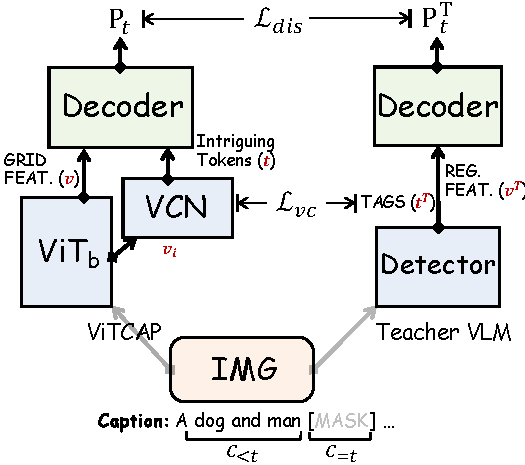
\includegraphics[width=.76\textwidth]{./images/distillation.pdf}
  \end{center}
  \vspace{-6mm}
    \caption[The overall training paradigm of ViTCAP.]{\small The overall training paradigm of ViTCAP can be understood as the knowledge distillation procedure where a detector-based Teacher VLM to assist the training of ViTCAP as a knowledge distillation paradigm. The CTN branch in ViTCAP learns to predict the semantic concepts as conceptual tokens for captioning. }
    \vspace{-2mm}
  \label{fig:distillation}
\end{figure}


\vspace{1mm}
\noindent \textbf{ViTCAP Architecture.} To give a more detailed explanation about the architecture of ViTCAP: it is consisted of a stem image encoder with $8$ transformer blocks (shared for both grid feature extractor and CTN), a CTN branch with $4$ transformer blocks, and a grid feature extractor with $4$ transformer blocks, the multi-modal module is also a $4$ transformer blocks module. When $M_1=12$, the model can be understood as consisting of two parallel branches, with one for concept prediction and one for grid representation. We does find that minimizing the shared blocks can bring extra performance gains but this inevitably increases the model size very obviously.
More experiments about different architectural instantiations are provided in the following.


\vspace{1mm}
\noindent \textbf{Architectural Variations.} We then experiment
with different architectural variations of ViTCAP and report their performances on COCO-caption in Table~\ref{tab:arch}. 
The baseline models include single-tower (SIN-TOW) that shares the ViT backbone for both modalities; Encoder-decoder (ENC-DEC) that use a ViT as visual encoder and 4 separate transformer blocks as modal fusion. This is similar to~\citep{kim2021vilt}, however we modify it with using seq-to-seq attention maps for the captioning training which prevents the model from seeing bidirectional context; Two-tower (TWO-TOW) uses an independent ViT/b architecture as conceptual token network and another architecture as the visual encoder; And VitCAP with different number of sharing blocks. We attach detailed architectures for these variations in the later section together with their learnable parameters. When adopting $8$ transformer blocks in the stem image encoder, we observe VitCAP achieves the close performances when $M_1=4$.



\vspace{1mm}
% \noindent\textbf{Evaluations on Google-CC and nocaps.}


% \section{Qualitative Examples}


\subsection{Discussions}
\noindent\textbf{Qualitative Examples.}
We demonstrate more qualitative examples of the attention maps produced by VitCAP together with their predicted semantic concepts in Figure~\ref{fig:qualitative}. 

\vspace{1mm}
\noindent\textbf{Can ViTCAP Ground Concepts?} Interestingly, we observe that the attention maps produced from transformer blocks closely relate to the concepts and various layers have different focuses while the averaged attention maps cover a broad holistic regions. We present more visualizations in Figure~\ref{fig:grounding} which contain single object per image for more direct analysis. The topmost row is a picture with multiple ``\texttt{wild gooses}'' and all regions of them are highlighted according to the attention maps. Despite so, it seems VitCAP suffers from identifying the clear borders of the object that it may only recognize part of the objects, \eg, ViTCAP only highlights the part of the ``\texttt{traffic light}'' and the ``\texttt{tie}''.

\vspace{1mm}
\noindent\textbf{VL Distillation Schema.} Our distillation schema can be indeed viewed as an extension of the VL distillation schema, where the Student model not only mimic the predicted masked token probability but also learns from the Teacher OD's object tags. As is shown in Figure~\ref{fig:distillation}. Note that our distillation technique is only applied on the \vitcap with VL pre-training, as the teacher VL model contains knowledge acquired from large scale pre-training and so it is unfair to compare the \vitcap with other methods without VL pre-training.

\begin{figure*}[t!]
%  \vspace{-3mm}
  \begin{center}
  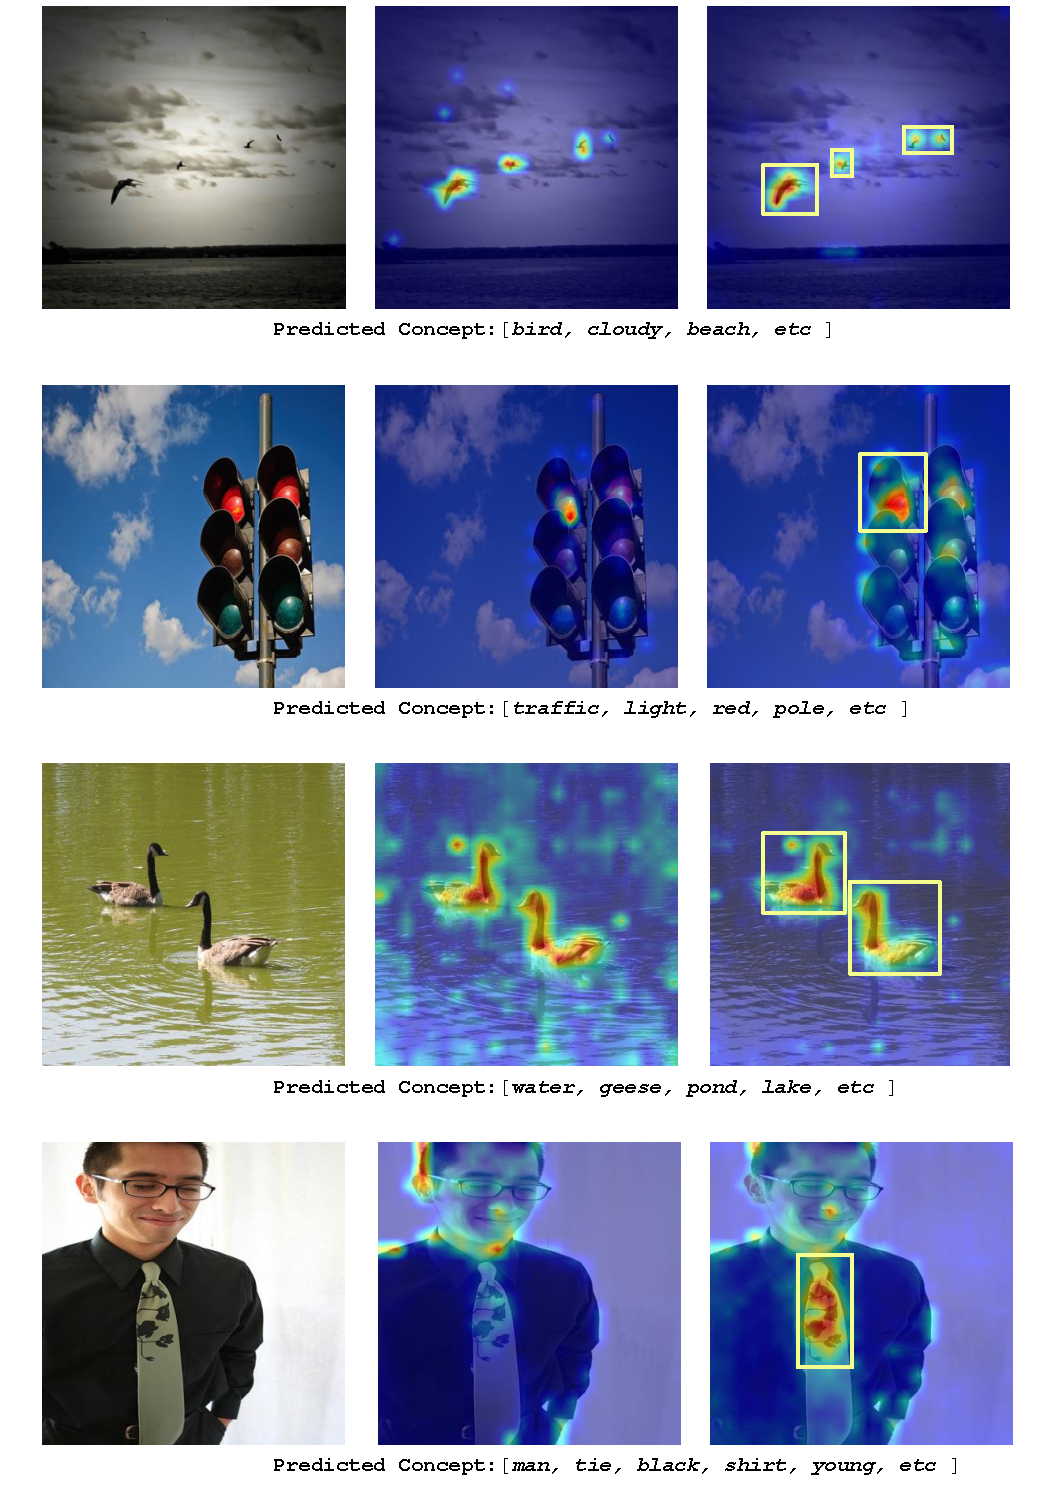
\includegraphics[width=.75\textwidth]{./images/grounding.pdf}
  \end{center}
  \vspace{-6mm}
    \caption{\small From left to right, we show the original image, average attention maps of the front 4 and 8 transformer blocks.  }
    \vspace{-2mm}
  \label{fig:grounding}
\end{figure*}



\vspace{1mm}
\noindent\textbf{Detector Tags \vs Caption Extracted Concepts.} Empirical studies show that the caption extracted concepts lead to better \vitcap\!. We conjecture that this is mainly because that the captions contain much broader image concepts contained in open-form texts, yet the detector tags are pre-defined with much more limited vocabulary. However, perfectly aligned image-text pairs are not always attainable considering that most existing image-level annotations are collected from Web. These image captions can be as noisy as alt text or short phrases, from which the extracted concepts only cover partial of the image content. Thus in practice, it is also an important aspect to explore the feasibility of adopting the non caption-extracted concepts, \eg, from an object detector as substitution. This provides a flexible source of the concepts. 




\subsection{Conclusion}
In this paper, we propose the ViTCAP, a detector-free image captioning model in the full transformer fashion. Compared with prior arts, \vitcap can be trained in an end-to-end fashion without intermediate regional operations using grid representations. Our proposed Concept Token Network learns broad semantic concepts and encodes them as the concept tokens that largely benefit the captioning task on a series of challenging captioning benchmarks. Extensive experiments indicate that \vitcap achieves competing performances, approaching most detector-based models. 

\vspace{-2mm}

% \include{chapter5}
% \include{chapter6}
% \include{conclusion}

                                        
{\singlespace
\addcontentsline{toc}{part}{REFERENCES}
\bibliographystyle{asudis}
% \bibliographystyle{ieeetr}
\bibliography{ref}
}

%\chapter{INTRODUCTION}
\pagenumbering{arabic}

\section{Overview}
The current progress in computer vision (V) and natural language processing (L) is inspiring. Representative V+L tasks include visual question answering (VQA), image/video captioning, textual grounding system, and image/video retrieval by language tasks. All these tasks have significant meanings to real-world applications: VQA and captioning systems can be the ground of cross-modal conversation systems, VL retrieval might be helpful for next-generation searching engines, and the textual grounding system helps to localize certain objects by open-form, and human-readable natural languages in robotics.


\begin{figure}
\begin{center}
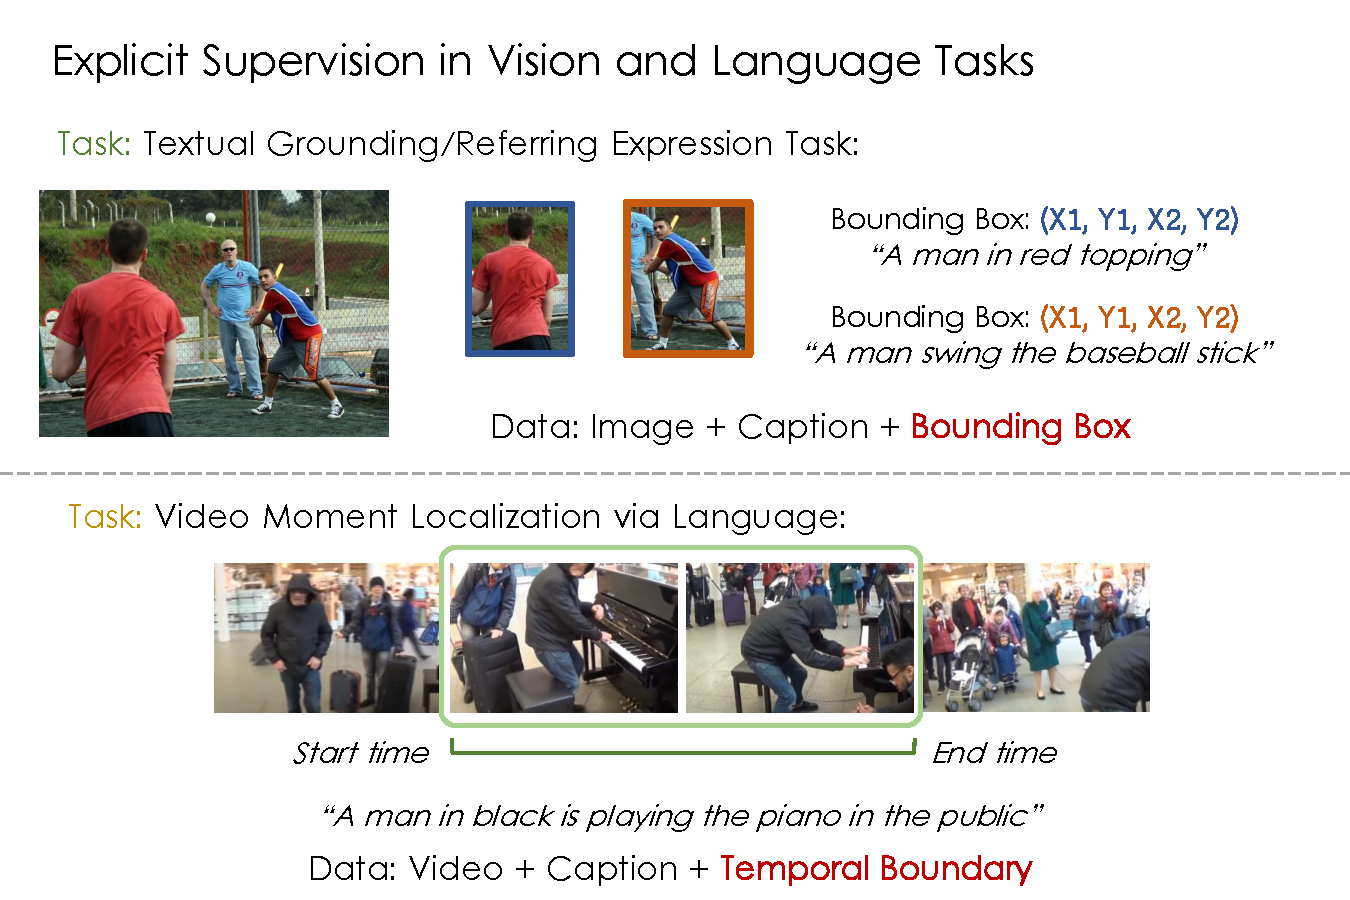
\includegraphics[width=.99\textwidth]{images/explicit_training.pdf}
\end{center}
\caption[Example of some VL tasks.]{VL tasks like textual grounding, referring expression and video moment localization via language unanimously require explicit annotations (\ie, bounding boxes of target objects or temporal boundaries for the moments) for learning of visual-textual correlation.
}
\label{fig:explicit_learning}
\end{figure}

Despite these, there exist several critical challenges that prevent us from pushing these advances to the real world.  One of the most difficult problems comes from the prohibitively expensive human labeling: previous powerful VL models are mostly domain-specific that rely heavily on a well-annotated VL dataset by humans, \eg, image captioning dataset like COCO~\citep{lin2014microsoft} collected  328K images, covering image-level object annotations and also captions explaining the content of images. Beyond that, the development of powerful VL systems like textual grounding models requires the awareness of spatial location per object (see Figure~\ref{fig:explicit_learning} for example). Compared with the countless images the system might encounter in the real world, annotating images at scale in COCO-style is hardly practical, nor financially effective. This spawns the challenge for the VL community: how to train a unified VL model that can be transferred to diverse domains via the implicit supervisions (\ie, large volume of weakly-annotated, or even un-labeled raw visual+textual data). Unlike the traditional vision model (object detection or recognition model), the VL model usually requires the understanding of correlations between visual concepts with rich semantics, while the traditional visual model only performs on a bunch of pre-defined and limited categories.


Another notable challenge arises when deploying the VL model on an edge device that usually has the limited computational power to be undertaken. It is impractical for real-world applications to exploit the power of prevailing VL models under a constrained training/inference budget due to their cumbersome sizes and huge computation cost. Building a lightweight VL model, meanwhile improving its performances is of great practical value but is less explored in the previous literature. In the furtherance of gaining a more real-world practical compact VL model, we study to exploit knowledge distillation techniques to improve the VL representation learning on compact models. 


Following the above-mentioned, I work on making contributions in the following aspects:

\begin{figure}
\begin{center}
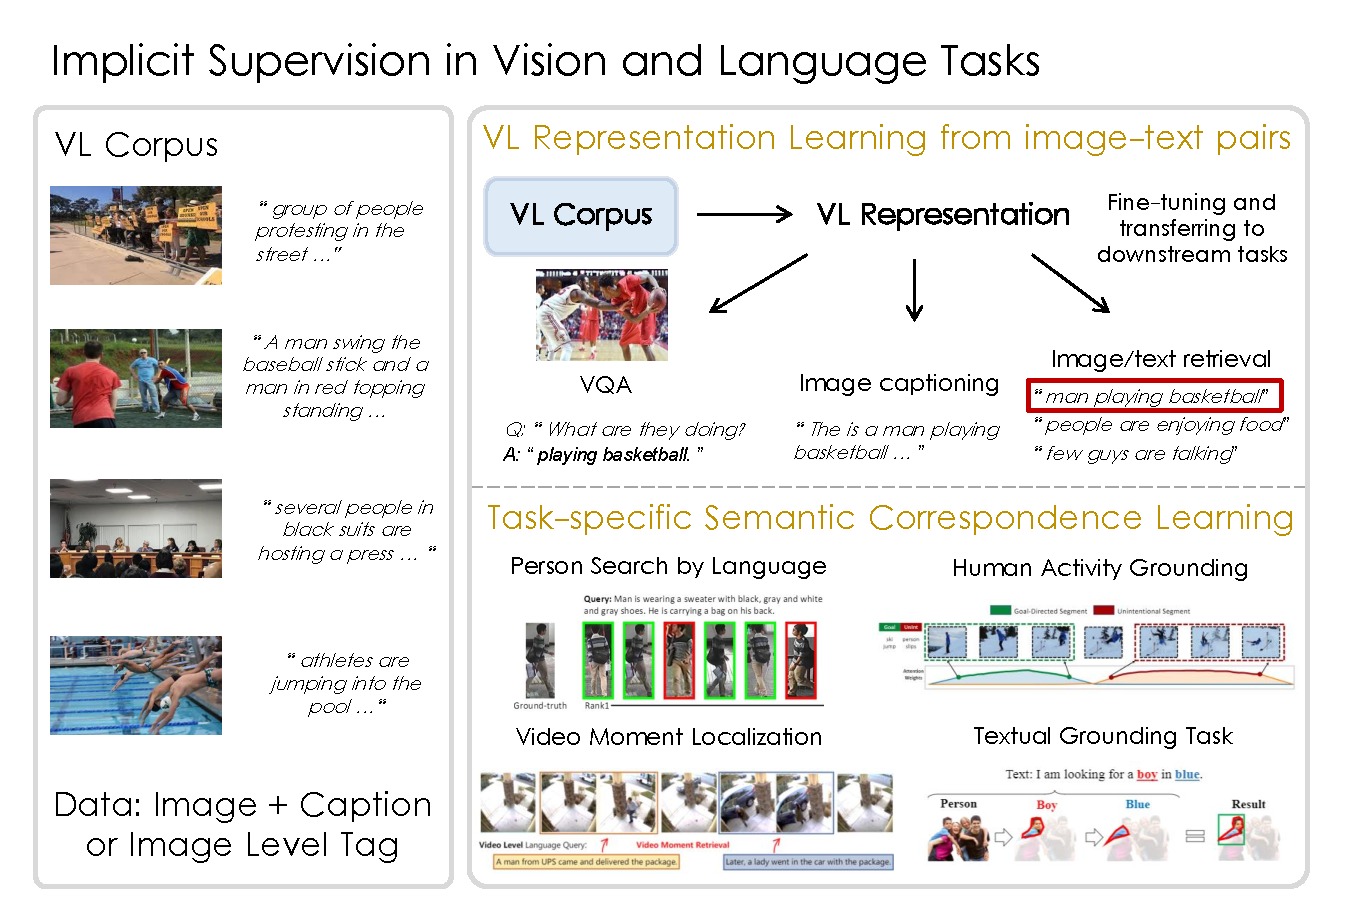
\includegraphics[width=.99\textwidth]{images/implicit_training.pdf}
\end{center}
\caption[VL Representation Learning \vs Downstream VL tasks.]{Unlike explicit VL supervisions, the training on implicit VL supervisions aims to learn either 1). task-agnostic and generic VL representations that can be transferred to other VL tasks, or 2). specific VL task (\eg, grounding, retrieval, etc). The former task focuses more on how to learn the VL representations from image-text pairs with better generalization and expressive semantics when there is no explicit training objective, while the latter requires a task-specific learning method (\eg, multi-instance learning).
}
\label{fig:implicit_learning}
\end{figure}

1. Learn the associations between visual concepts and semantics in a weak/un-supervised fashion. For example, when given an image, learn which specific region best corresponds to a textual query ``\textit{A man in red topping}'', when we have only an image-level general description like ``\textit{A man swing the base ball stick and a man in red topping standing in the playground ...}'', without knowing the exact region corresponds to specific visual concepts (a.k.a, weakly-supervised textual grounding in images/videos).

2. Learn ``omni''-VL representations that can be transferred to diverse VL tasks from image-text pairs via pre-training and fine-tune fashion. Now as the VL pre-training leverages only general image+text pairs without further spatial, or pixel-level annotations, it is challenging how to effectively mine the hidden visual-textual associations at scale for representation learning (as is shown in Figure~\ref{fig:implicit_learning}). Beyond that. I also work on leveraging task-agnostic knowledge distillation in assisting the representation learning on small and generic VL models. 

3. Build an efficient VL model. Much of the existing VL models focus on large models that suffer from high latency and large memory footprints at the time of inference, which limits their deployment to resource-constrained edge devices for real-world applications. I study how to train small and efficient VL models from the perspective of Knowledge Distillation for model compression. In the end, I explain the feasibility of developing the ``one-stage VL model'' which does not require the cumbersome object detector and thus brings obvious flexibility for both model training and inference. 

% Figure~\ref{fig:explicit_learning} gives an overview of the major aspects of this dissertation. 
This dissertation highlights a few selected research projects I worked on from the aforementioned perspective: 1). A textual grounding system that learns the semantic correspondence from weakly supervised learning~\citep{Fang_2019_CVPR,fang2019temporal}. 2). A novel self-supervised visual representation learning paradigm coupled with knowledge distillation~\citep{fang2020seed}. 3). A compact VL model that benefits from VL distillation, which can be transferred to a series of other generic downstream VL tasks~\citep{fang2021compressing}. Also an one-stage image captioning model that brings training flexibility and inference speed~\citep{fang2021injecting}. All of these efforts reflect my primary research in the intersection of computer vision and natural language processing that advances the V+L learning from implicit supervisions with increased efficiency.

\section{Preliminaries}
To give the readers a more comprehensive background introduction about the Vision and Language and some relevant techniques this dissertation mentions later, I will briefly review several Vision Language tasks, together with their formulation under the weakly-supervised learning schema. These weakly-supervised VL tasks are less data-dependent than they attempt to learn the cross-modal correspondence without explicit supervision. Nevertheless, they are inevitably limited to only specific VL tasks that need manual design. To circumvent these, a broader series of works alter to introduce the generic representation learning from a large VL corpus that their ``omni''-representations are transferable to different downstream tasks and are entirely task-agnostic during the pre-training phase.

\subsection{Glance of Prevailing VL Tasks}


\begin{figure}
\begin{center}
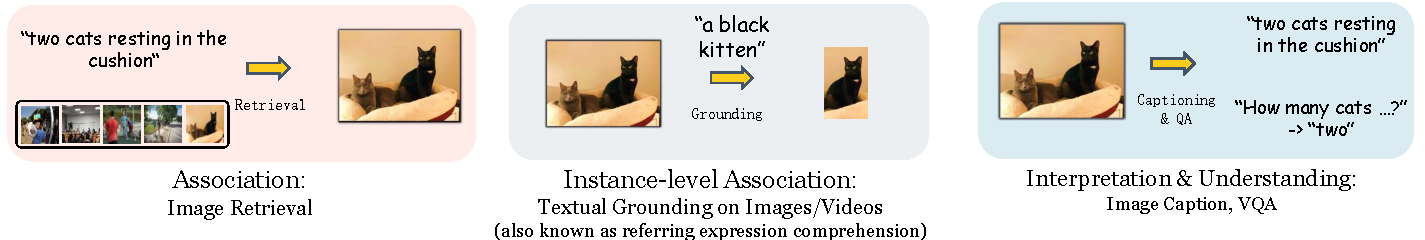
\includegraphics[width=.99\textwidth]{images/VL-tasks.pdf}
\end{center}
\caption[Prevailing VL Tasks.]{Glance of some representative VL tasks from different perspectives. The image content retrieval task builds upon the association relationship across the Vision and Language modalities. Proceeding from that, this association extends to the instance-level that one can retrieve either a region of the image covering a specific object or a short video moment containing an event in untrimmed video. High-level VL tasks involve more interpretation and understanding: for instance, generating a textual description from the observation, or answering the question based on the visual observation.}
\label{fig:VLtasks}
\end{figure}

\noindent{\bf Association Learning across Vision and Language} is core and tie of a wide range of tasks across vision and language domains, \emph{e.g.}, textual grounding~\citep{plummer2015flickr30k}, referring expression comprehension~\citep{nagaraja2016modeling} or object retrieval using language~\citep{hu2016natural}. In particular, given an image $\mathbf{I}$, {T}extual {G}rounding model selects a proposal $\mathbf{c}$ given a textual query $\mathbf{T}$ from a set of coordinates $\mathbf{C} = \{\mathbf{c_1 \dots c_N}\}$ (see example in Figure~\ref{fig:VLtasks}):
\begin{equation}
    \mathbf{c} = \text{Textual-Grounder}{\big(}\mathbf{I}, \mathbf{T},\mathbf{C}{\big)},
\end{equation}
where $N$ denotes the number of candidate proposals generated by some generic proposal network. To obtain a strong textual grounding model, one might need to collect massive \texttt{<image-text-proposal>} triplets to sufficiently train such a model. 
Such association learning also extends to the video domains ({V}ideo {L}ocalization Task) where the textual description is utilized as the query to anchor a clip from a long untrimmed video:
\begin{equation}
    \mathbf{c} = \text{Moment-Localizer}{\big(}\mathbf{V}, \mathbf{T}, \mathbf{C}{\big)},
\end{equation}
where now the proposal $\mathbf{c}$ is selected as the temporal boundary of a video moment with starting time $t_s$ and ending time $t_e$ of the video $\mathbf{V}$.

Recent works shed light on the importance of leveraging the image-level annotations (as weak supervision)~\citep{fang2018modularizedtextual,fang2018weakly} or unsupervised method~\citep{yeh2018unsupervised} to learn the association across language descriptions and objects. Proceeding from this, there arise works on using uncurated captions to learn temporal associations across video segments and texts~\citep{miech2019end,sun2019videobert}. Notably, these works all highlight the importance of constructing contrastive pairs in exploiting the weak annotations. We will discuss more about the contrastive learning at later section. 

\noindent{\bf Visual Interpretation via Language} tasks laid more emphasis on the high-level understanding aspects. Typical interpretation tasks include \emph{Visual Captioning} and \emph{Visual Question Answering} Tasks (an example is shown in Figure~\ref{fig:VLtasks}). Visual captioning is perhaps the first step towards understanding images/videos and describing their content in natural language.
Recent advances in visual captioning have been able to generate captions that describe humans and objects and their interactions in the video.
They seek to generate paragraphs or multi-sentence captions about the content of images or videos.
It is important to note that visual captioning systems have a major limitation in that they can only generate factual descriptions about observable objects or events in the video yet without full \emph{understanding} the content. For detailed visual understanding, we would like to go beyond observable visual entities and use background knowledge and contextualization to reason about the observation and answer the questions. Most existing VQA benchmarks only predict answers from a pre-constructed \& limited answer sets, largely limits the practical scopes of the systems. Few recent works propose the open-domain VQA task~\citep{chang2021webqa} that generates the answers directly, or the VQA tasks need external knowledge~\citep{wang2017fvqa,zellers2019vcr,marino2019ok,garcia2020knowit,7298682}


\subsection{Implicit Supervisions for VL Tasks}
\noindent{\bf Weakly Supervised Learning} receives increasing attention~\citep{deselaers2010localizing,pandey2011scene, cinbis2017weakly,mahajan2018exploring,pathak2015constrained,pinheiro2015image,xu2014tell}.
It focuses on learning granular detectors given only coarse annotations.
This is of practical significance as granular annotations (\eg, bounding boxes and pixel-level labels) are much more expensive to obtain compared to coarse image-level annotations.
Recent studies show that weakly supervised methods can even outperform the strongly supervised method for image classification~\citep{mahajan2018exploring,ge2019weakly},
and is even widen to a wide range of vision tasks, including object detection~\citep{bilen2014weakly,shen2018generative,bilen2016weakly}, semantic segmentation~\citep{kervadec2019constrained,pathak2015constrained,wei2016stc} and etc.
In video analysis domain, the weakly-supervised action localization is frequently studied and can be thought of a specific example of learning with the video-level labels~\citep{sun2015temporal,shou2018autoloc,nguyen2018weakly,paul2018w}.
This problem derives from the fully-supervised counterpart methods which exploits fine annotations at frame level
for localizing the actions~\citep{buch2017sst,kalogeiton2017action,weinzaepfel2015learning,shou2017cdc,tran2012max,shou2016temporal}.
Recent weakly-supervised methods extensively adopt either the video-level classification framework~\citep{singh2017hide,shou2018autoloc,sikka2014classification,dwibedi2019temporal} or with the attentional mechanism 
that generates bottom-up sparse weights used for localizing action categories temporally~\citep{nguyen2018weakly}. Beyond that, few works~\citep{wang2017untrimmednets,paul2018w} propose to utilize the multi-instance learning loss to address this challenge,~\citep{paul2018w} also suggests exploiting the co-activity across videos in the metric learning, which largely improves the action localization task even when temporal annotations are not available. The most recent work~\citep{nguyen2019weakly} improves over these methods with a background modeling module that explicitly extracts the foreground and background appearances.  This dissertation focus more on extending this weakly supervised learning signals to VL tasks.\footnote{Implicit supervisions in this dissertation refer to both weakly-supervised learning and self-supervised learning.}

% Unlike current work,
% we perform weakly-supervised learning for textual grounding, including training for both entity grounding
% and textual-visual matching through a progressive modular procedure.

% Modular design is also receiving more attention recently, mainly for
% complex systems like visual-question-answering or image captioning~\citep{hu2017modeling, hu2018explainable,
% yu2018mattnet}.
% Such modular design is carried out by realizing some linguistic structures.
% In our work,
% we propose to decompose the query textual description into progressive levels,
% each of which is passed to a corresponding module,
% and then produce the final grounding result by progressively merging the intermediate results.
% In this way,
% our system enjoys high interpretability and resilience to counterfactual inputs.

% Few works also shed light upon the importance of contrastive learning for weak supervision.


\noindent{\bf Weakly-Supervised Image/Video Grounding by Language} 
We are concerned with the model's dependency on the complicated data annotations for textual grounding task. For this reason, it is important to study how to build 

Temporal Grounding and Moments Retrieval are two instantiations of learning
temporal-textual association.
In these tasks, most recent methods adopt fully-supervised training over 
fine annotations on the frame-textual associations.
For example, Gao \emph{et al.} augment the Charades 
dataset~\citep{sigurdsson2016hollywood} by generating complex language queries with temporal boundary annotations for language moment retrieval~\citep{gao2017tall}; 
Anne Hendricks \emph{et al.} also collect a new dataset for training to localize video moments over a given descriptive sentence~\citep{anne2017localizing}. 
Other follow-up methods~\citep{hendricks2018localizing,liu2018attentive,chen2018temporally,wang2018bidirectional,xu2019joint,gavrilyuk2018actor} also
fully-supervised train for temporal grounding using these datasets,
suffering from the limitation on their generalizability due to  
the combinatorial nature of complex natural language sentences (\textit{e.g.}, 
synonymous words, grammatical tense 
and sentence structures)~\citep{hendricks2018localizing,gao2017tall}. 
advances the aforementioned to an even challenging task, as now the only available supervision is video-level natural language descriptions in an open format, which come with a huge amount of unnecessary noises.
In particular, Mithun \emph{et al.}~\citep{Mithun_2019_CVPR} for the first time attempted to 
solve the temporal grounding problem by weakly supervising learning 
with only the video-level textual queries~\citep{Mithun_2019_CVPR}. 
In~\citep{chen2020look}, the author proposed to utilize the temporal proposal and textual description alignment learning using the sliding window fashion and tackle the grounding problem in a coarse-to-fine manner. Similarly, a very recent work by~\citep{lin2019weakly} also focuses on the design of a better proposal generation module, that aggregates the contextual visual cues to generate and score the proposed candidates for grounding. We summarize that current efforts in weakly supervised language grounding are either centered on better proposal generation~\citep{chen2020look,lin2019weakly} or a better cross-modal association model by constructing contrastive samples across video and languages~\citep{Mithun_2019_CVPR,gao2019wslln}. Our WSRA (introduced in later Chapter) places emphasis on the latter, but nevertheless further distinguishes the above with a more comprehensive cross-modal association learning objectiveness and a novel sampling and weighting strategy in our metric learning step.

\subsection{VL Representation Learning from Weak Annotations}

Following the prominent progress in the transformer-based (introduced in later section)~\citep{vaswani2017attention} pre-training in natural language~\citep{devlin2018bert,radford2018improving,lagler2013gpt2,brown2020language,clark2020electra,raffel2019exploring}, Vision Language pre-training models, either for image+text~\citep{lu2019vilbert,tan2019lxmert,chen2019uniter,li2020oscar,hu2020vivo,zhang2021vinvl,li2020closer,gan2020large,li2020hero,lu202012} or for video+text~\citep{sun2019videobert,li2020hero,miech2020end,zhu2020actbert,lei2021less}, have achieved great success on a number of downstream V+L tasks. 

\subsection{Self-supervised Learning and Contrastive Learning}
Another important implicit supervision is the self-supervised learning technique. 
Among the recent works in \textbf{Self-supervised Learning (SSL)}, contrastive based approaches show prominent results on downstream tasks. Majority of the techniques along this direction are stemming from noise-contrastive estimation~\citep{gutmann2010noise} where the latent distribution is estimated by contrasting with randomly or artificially generated noises. 
~\citep{oord2018representation} first proposed Info-NCE to learn image representations by predicting the future using an auto-regressive model for unsupervised learning. Follow-up works include improving the efficiency~\citep{henaff2019data}, and using multi-view as positive samples~\citep{tian2019contrastive1}. As these approaches can only have the access to limited negative instances,~\citep{wu2018unsupervised} designed a memory-bank to store the previously seen random representations as negative samples, and treat each of them as independent categories (instance discrimination). However, this approach also comes with a deficiency that the previously stored vectors are inconsistent with the recently computed representations during the earlier stage of pre-training. ~\citep{chen2020simple} mitigate this issue by sampling negative samples from a large batch. Concurrently,~\citep{he2020momentum} improve the memory-bank based method and propose to use the momentum updated encoder for the remission of representation inconsistency. Other techniques include~\citep{misra2020self} that combines the pretext-invariant objective loss with contrastive learning, and ~\citep{wang2020understanding} that decomposes contrastive loss into alignment and uniformity objectiveness.


\subsection{Knowledge Distillation}
Knowledge Distillation has been applied to model compression task across different domains with its main goal being to transfer the ``\textit{knowledge}'' $f(x_i)$ of sample ($x_i, y_i$) from a strong Teacher network ($T$) to the Student network ($S$) by minimizing the divergence between them:
\begin{equation}
\mathcal{L} = \frac{1}{N}\sum_{i=1}^{N}\bigg(\mathcal{L}_\text{S}(x_i, y_i) + \mathcal{L}_\text{KD}\Big(f^S(x_i), f^T(x_i)\Big)\bigg),
\end{equation}
where $\mathcal{L}_\text{S}(\cdot)$ refers to the original supervision signal(s) on the Student. In practice, this term can possibly be replaced by the exclusive use of $L_\text{KD}$. Depending on the type of knowledge transferred, $\mathcal{L}_\text{KD}$ can derive from soft cross-entropy, mean squared error (MSE) function or \textit{KL}-divergence.
For example,~\citep{hinton2015distilling,bucilua2006model} transfer the learned knowledge by mimicking the mass function of the output probability across classes, or by minimizing the divergence of intermediate features~\citep{yim2017gift,koratana2019lit,huang2017like,yalniz2019billion,xie2020self}.
Works in ~\citep{ahn2019variational,yim2017gift,koratana2019lit,huang2017like} have utilized different learning objectives including consistency on feature maps, consistency on probability mass function, and maximizing the mutual information. CRD~\citep{tian2019contrastive}, which is derived from CMC~\citep{tian2019contrastive1}, optimizes the student network by a similar objective to~\citep{oord2018representation} using a derived lower bound on mutual information. 
~\citep{tian2019contrastive,tian2019contrastive,fang2021seed} propose contrastive distillation for visual representation learning.  In addition, remarkable advances have been made in knowledge distillation for language model compression (\ie, BERT~\citep{devlin2018bert}), and these works show that mimicking the distribution of self-attention and intermediate representations of transformer blocks increases performances~\citep{sanh2019distilbert,jiao2019tinybert,sun2020mobilebert,xu2020bert} for downstream tasks.
In particular, in the transformer-based language model distillation, DistillBERT~\citep{sanh2019distilbert} proposes to train the small BERT by mimicking the Teacher's output probability of masked language prediction and the embedding features.  TinyBERT~\citep{jiao2019tinybert} and MobileBERT~\citep{sun2020mobilebert} leverage the layer-wise attention distributions for distillation with MSE function.~\citep{wang2020minilm} suggests distilling on the last transformer layer and bringing extra flexibility for training.~\citep{sun2020contrastive,chen2020wasserstein} also use the contrastive distillation in transformer-based language model compression.~\citep{fang2021seed,sun2020contrastive} propose using a sample queue to store history embeddings and show that contrasting with more negative samples is beneficial for knowledge distillation. 

\subsection{Architecture of VL Model}
Most existing VL models are designed in a two-step fashion: a pre-trained object detector is used to encode the image as
set of regional features (as offline visual tokens) followed by pre-training on a large scale visual-linguistic corpus using tasks like masked language modeling, image-text matching or masked region modeling losses. In particular, Zhang \etal~\citep{zhang2021vinvl} demonstrate the significant role of visual features in VL pre-training and looks for more effective visual representations from a larger object detector. Li~\etal~\citep{li2020oscar} shows that a larger transformer VL model can learn better from larger VL corpus. However, the marginal costs are greater than the marginal benefits. 
Recently, Wang \etal~\citep{wang2020minivlm} propose a small VL model called MiniVLM that uses a lightweight visual feature extractor and smaller transformer to reduce the model size by 73\% and maintain good accuracy on VL tasks. 
Nevertheless, the cost of pre-training on MiniVLM is associated with sub-optimal efficiency: it requires a large amount of training data (14M) to learn a good representation. Thus, it is worth exploring a more efficient way to train small VL models. 
There are other lines of VL pre-training works in which grid features~\citep{huang2020pixel,jiang2020defense} is extracted from the convolutional layers without the proposal computation.~\citep{ramesh2021zero,radford2021learning,desai2020virtex} learn visual representation from scratch using Convolutional Neural Network as image encoder with a transformer for VL pre-training on a large amount of image-text pairs.  The notion of VL distillation is not limited to just the two-stage VL models, it can potentially benefit other types of transformer-based VL models as well. 



\begin{figure}[t]
\centering
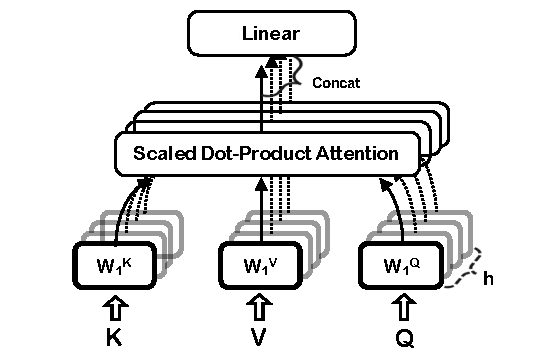
\includegraphics[width=.45\textwidth]{./images/attention.pdf}
\caption{ Illustration of Multi-Head Attention block. Each block consists of $L$ attention layers. 
}
\label{fig:multiattention}
\end{figure} 

\subsubsection{Transformer Model}
A Transformer Model is composed of a stack of identical transformer blocks, whose main component is a self-attention architecture.
It takes as input the summation of word embedding and the positional encoding offset by 1 position through a masked multi-head attention block, which prevents future words from being seen by the block. 

The transformer block consists of several consecutive linear transformations.
Let $\mathcal{H}_{\textsc{M-Att}}$ denotes the multi-head attention block, $\mathcal{H}_{\textsc{Norm}}$ be the normalization layer and $\mathcal{H}_{\textsc{FFN}}$ be the feed forward layer.
Let K, V, and Q denote the key, value, and query respectively, which are inputs to the attention block.
The transformer block can be summarized as follows:
\begin{equation}
\begin{split}
\tilde{o_1}^\ell&=\mathcal{H}_{\textsc{M-Att}}(\textrm{K}, \textrm{V}, \textrm{Q}) \\
\tilde{o_2}^\ell &= \mathcal{H}_{\textsc{Norm}}(\tilde{o_1}^\ell + \tilde{\mathbf{o}}^{\ell-1})   \\
\tilde{o_3}^\ell &= \mathcal{H}_{\textsc{FFN}}(\tilde{o_2}^\ell)   \\
\tilde{o}^{\ell}&= \mathcal{H}_{\textsc{Norm}}(\tilde{o_3}^\ell \tilde{o_2}^\ell),
\end{split}
\end{equation}
In the context of the transformer blocks used in our work, the video encoding acts as the key, the concatenation of video/caption encoding is the value, and the output from the previous transformer block acts as the query.


\subsubsection{Multi-head Attention Block}
\label{sec:att_block}
In the masked multi-head attention block, the transformer block is used with K, V, and Q being identical vectors of the input embedding.
An example of a multi-head attention block is shown in Figure~\ref{fig:multiattention}.
The motivation of the design originates from the self-attention mechanism that aims to solve the problem of long-term dependencies because of which the propagated gradients tend to vanish or explode. 
    Instead of handling sequences word by word, the self-attention block learns the attention weight between every word and produces a representation with a global view of the input.
A self-attention block with $L$ heads is formulated as: 
\begin{equation}
\mathcal{H}_{\textsc{M-Att}}(\textsc{K}, \textsc{V}, \textsc{Q}) = \mathcal{H}_{\textsc{FFN}}([{g_1}, {g_2}, ..., {g_L}]).
\end{equation}
$g_i$ for every head-index $i$ is computed by a scaled dot-product attention operation as:

\begin{equation}
{g_i} = \textsc{Softmax}\xbigg(\frac{\textsc{w}^\textsc{q}_i \textsc{Q}\cdot \textsc{w}^\textsc{k}_i \textsc{K}^\prime}{\sqrt{d_k}}\bigg)\textsc{w}^\textsc{v}_i \textsc{V}, \forall i \in \{1, \dots, L \},
\end{equation}
where $d_k$ is the dimension of keys, and $\textsc{w}_i$ are the learnable parameters of the linear transformation.

% \section{Related Literature}


In what follows, we will introduce our progress towards each perspective as stated above. In Chapter 2, we summarize our effort to build a VL grounding model from weak supervisions, achieving satisfactory grounding results compared with explicit supervised models. Furthermore, we also investigate the effort of extending the weakly-supervised grounding to videos. In Chapter 3, we then introduce a novel self-supervised visual representation learning algorithm that is facilitated by knowledge distillation technique which achieves major performance gain. We extend this contrastive learning-based distillation algorithm to the VL representation learning on a small VL architecture. Chapter 4 presents a one-stage VL model that is object detector-free and can be end-to-end optimized dubbed ViTCAP, experiment shows that our ViTCAP reaches state-of-the-art image captioning performances amongst all existing one-stage VL models. We finally summarize our work and point some future research directions in the end.                     %<Insert your chapters here; I recommend to use
%% \chapter{Visual-linguistic Semantic Correspondence from Weak Supervisions}
\chapter{VL SEMANTIC CORRESPONDENCE FROM WEAK SUPERVISIONS}


Visual recognition understands the content of image by categorizing the target object from pre-defined classes. Treating such problem as a classification task narrows the scope of what machines can recognize due to the limited data and computing power.
Language, however, contains large-scale and plentiful textual descriptions about the attributes, states, or even underlying aspects about the target object or scenes. For example, the textual phrase ``\textit{a boy in blue shirt}'' does not only implies of the existence of person, while also indicating the gender, age and the color of the dress on the target object. The utilization of open-form sentences enables the grounding system to localize object in a greater scope and flexibility. 
Though textual description does not always precisely and comprehensively covers the content of the image, such data always couples with ``large-scale'' and ``weak'' labels. This chapter studies how to better leverage and exploit textual data as weak supervision and find the image region (or video moment) that best matches the textual descriptions when no bounding box (or temporal boundary) annotations.
This chapter contains several works for the textual grounding on image, video moment/activity localization by language tasks all in a weakly-supervised learning fashion for semantic correspondence capturing.

\section{Associating V to L without Explicit Supervisions}
Multi-modal tasks, \eg. assistive visual search~\citep{cai2004hierarchical, la1998combining}  and image captioning~\citep{you2016image, vinyals2017show}, has been studied for decades in the community. While those tasks are classical topics in computer vision and natural language processing,
current advancement has further energized it by interplaying
vision (images) and language (high-level guide) for practical applications. Specific examples include referring expressing understanding~\citep{nagaraja2016modeling,hu2017modeling} and reasoning-aware visual-question-answering~\citep{hu2017learning}.

State-of-the-art textual grounding methods \citep{yu2018mattnet, hu2016natural, rohrbach2016grounding, plummer2015flickr30k, yeh2017interpretable, luo2017comprehension, fang2018weakly} are based on deep neural networks and relying on
large-scale training data with manual annotations for the object bounding box and relationship between
phrases and figures/objects.
This setup largely limits their broad applications as such strong supervision is expensive to obtain,
and they also lack interpretability and resilience to counterfactual cases which do not appear in training.




\section{Weakly-Supervised Textual Grounding on Images}

\begin{figure*}[h]
  \begin{center}
    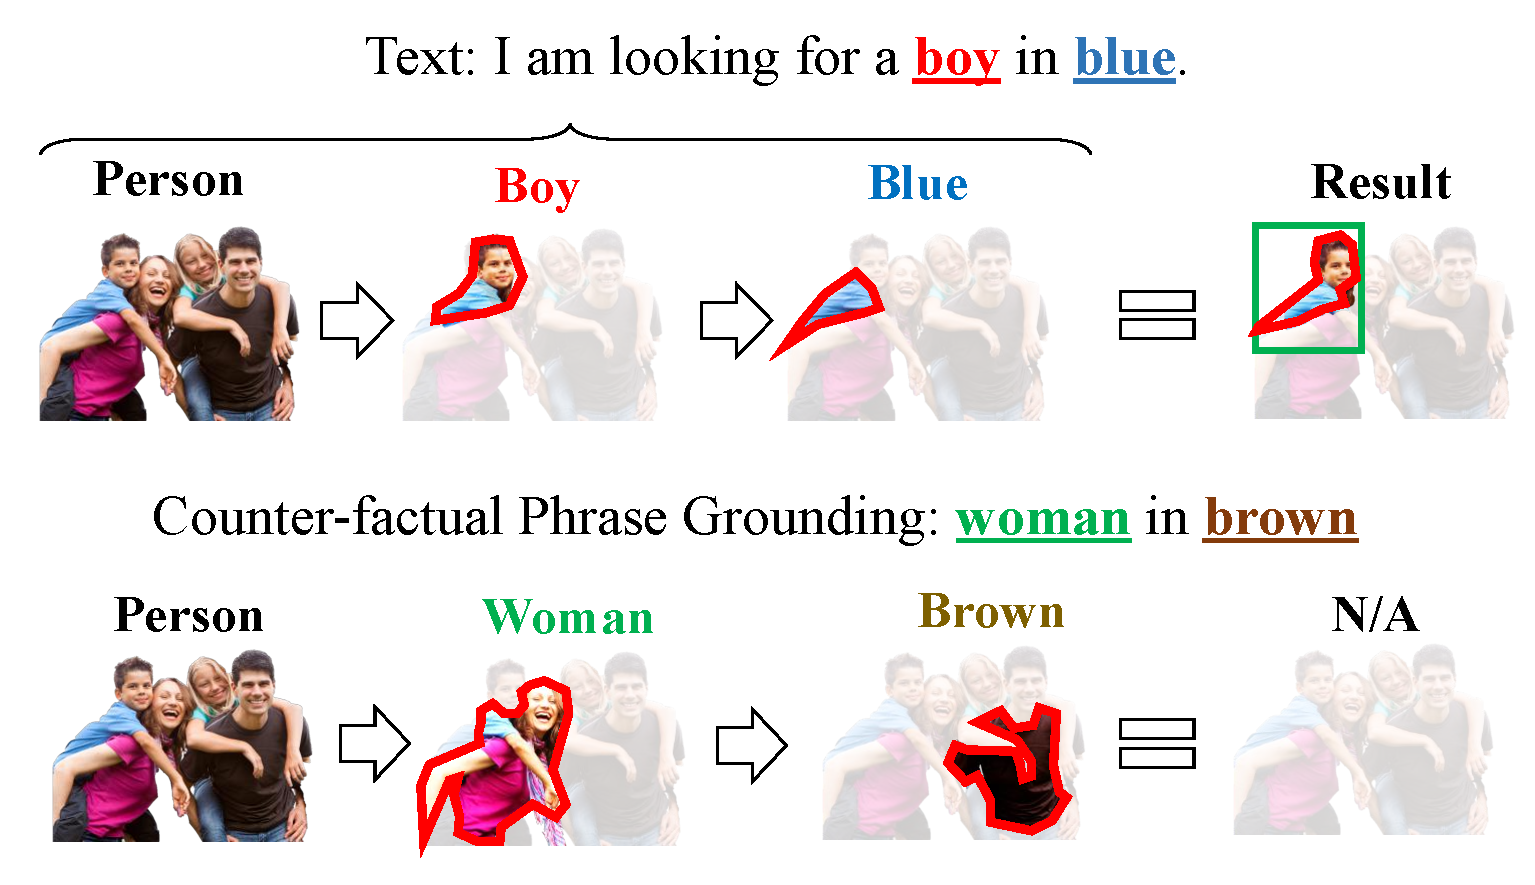
\includegraphics[width=1.0\textwidth]{images/mtg_abstract.pdf}
  \end{center}
  \caption{A example of textual grounding system, where the visual concepts are localized by open-form textual description, thus enabling the system to interact with users with high flexibility.}
  \label{fig:grounding}
 \end{figure*}

Computer Vision applications often require a textual grounding module with precision, interpretability, and resilience to counterfactual inputs/queries. To achieve high grounding precision, current textual grounding methods heavily rely on large-scale training data with manual annotations at the pixel level. Such annotations are expensive to obtain and thus severely narrow the model's scope of real-world applications. Moreover, most of these methods sacrifice interpretability, generalizability, and they neglect the importance of being resilient to counterfactual inputs. To address these issues, we propose a visual grounding system which is 1) end-to-end trainable in a weakly supervised fashion with only image-level annotations, and 2) counterfactually resilient owing to the modular design. Specifically, we decompose textual descriptions into three levels: entity, semantic attribute,  color information, and perform compositional grounding progressively. We validate our model through a series of experiments and demonstrate its improvement over the state-of-the-art methods. In particular, our model's performance not only surpasses other weakly/un-supervised methods and even approaches the strongly supervised ones, but also is interpretable for decision making and performs much better in face of counterfactual classes than all the others.


\begin{figure*}[t]
\begin{center}
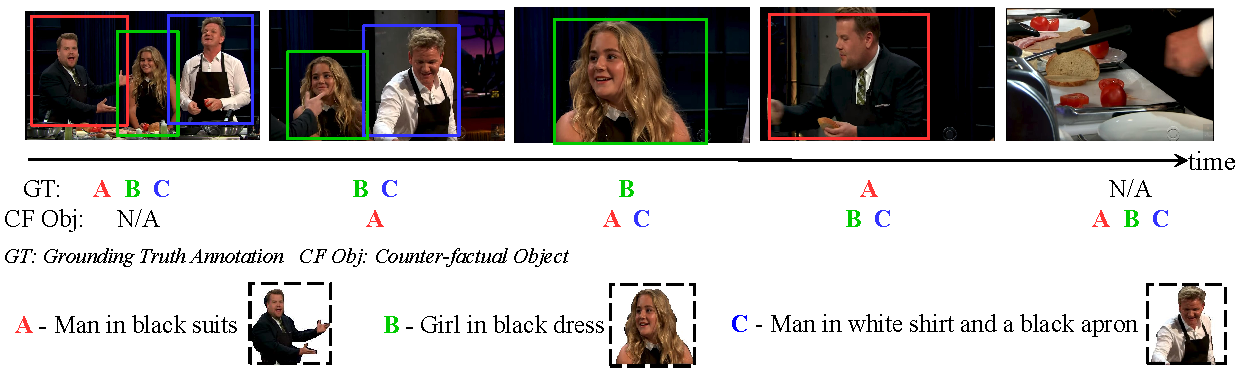
\includegraphics[width=1.0\linewidth]{images/ca_demo.pdf}
\end{center}
\caption{Example of the counter-factual object grounding.}
\label{fig:ca_demo}
\end{figure*}


\subsection{Modularized Textual Grounding Model with Weakly-supervised Training}
To obtain better interpretability and counterfactual resilience,
we propose to modularize the our whole textual grounding system
by decomposing the textual descriptions into multiple levels,
each of which is passed to a specific module to process.
We generate the final grounding result by progressively merging intermediate
results from these modules.

Without losing generalization,
in this work,
we decompose the textual descriptions into three levels,
and progressively process them with three different modules, respectively:
entity grounding module $M_e$,
semantic attribute grounding module $M_a$, and color grounding module $M_c$.
We extracted phrases and words that belong to such three levels from text, and feed them into their corresponding sub-modules.
We note that such a modular design allows for training different modules using different specialized protocols,
e.g., fully supervised learning or weakly supervised learning,
while also enables end-to-end training.
For the final grounding heat map $G$,
we merge progressively the intermediate results from these modules as below (see Figure \ref{fig:pipeline}):
\begin{equation}
\begin{split}
G & = M_e \cdot (M_a + M_c).
\label{eq:att}
\end{split}
\end{equation}

In practice, we observe that such a merging approach achieves the best
performance, better than the straightforward multiplicative or additive fusion.
This is because that the entity grounding sets the object constraints, and the summation
over the attribute and color modules interpretably delivers how the final results are generated,
though they may partially cover some regions belonging to the object of interest.
In the remaining of this section,
we elaborate each of the three modules and the adopted training protocols.



\subsubsection{Entity Grounding Module (M$_{e}$)}


\begin{figure*}[t]
\begin{center}
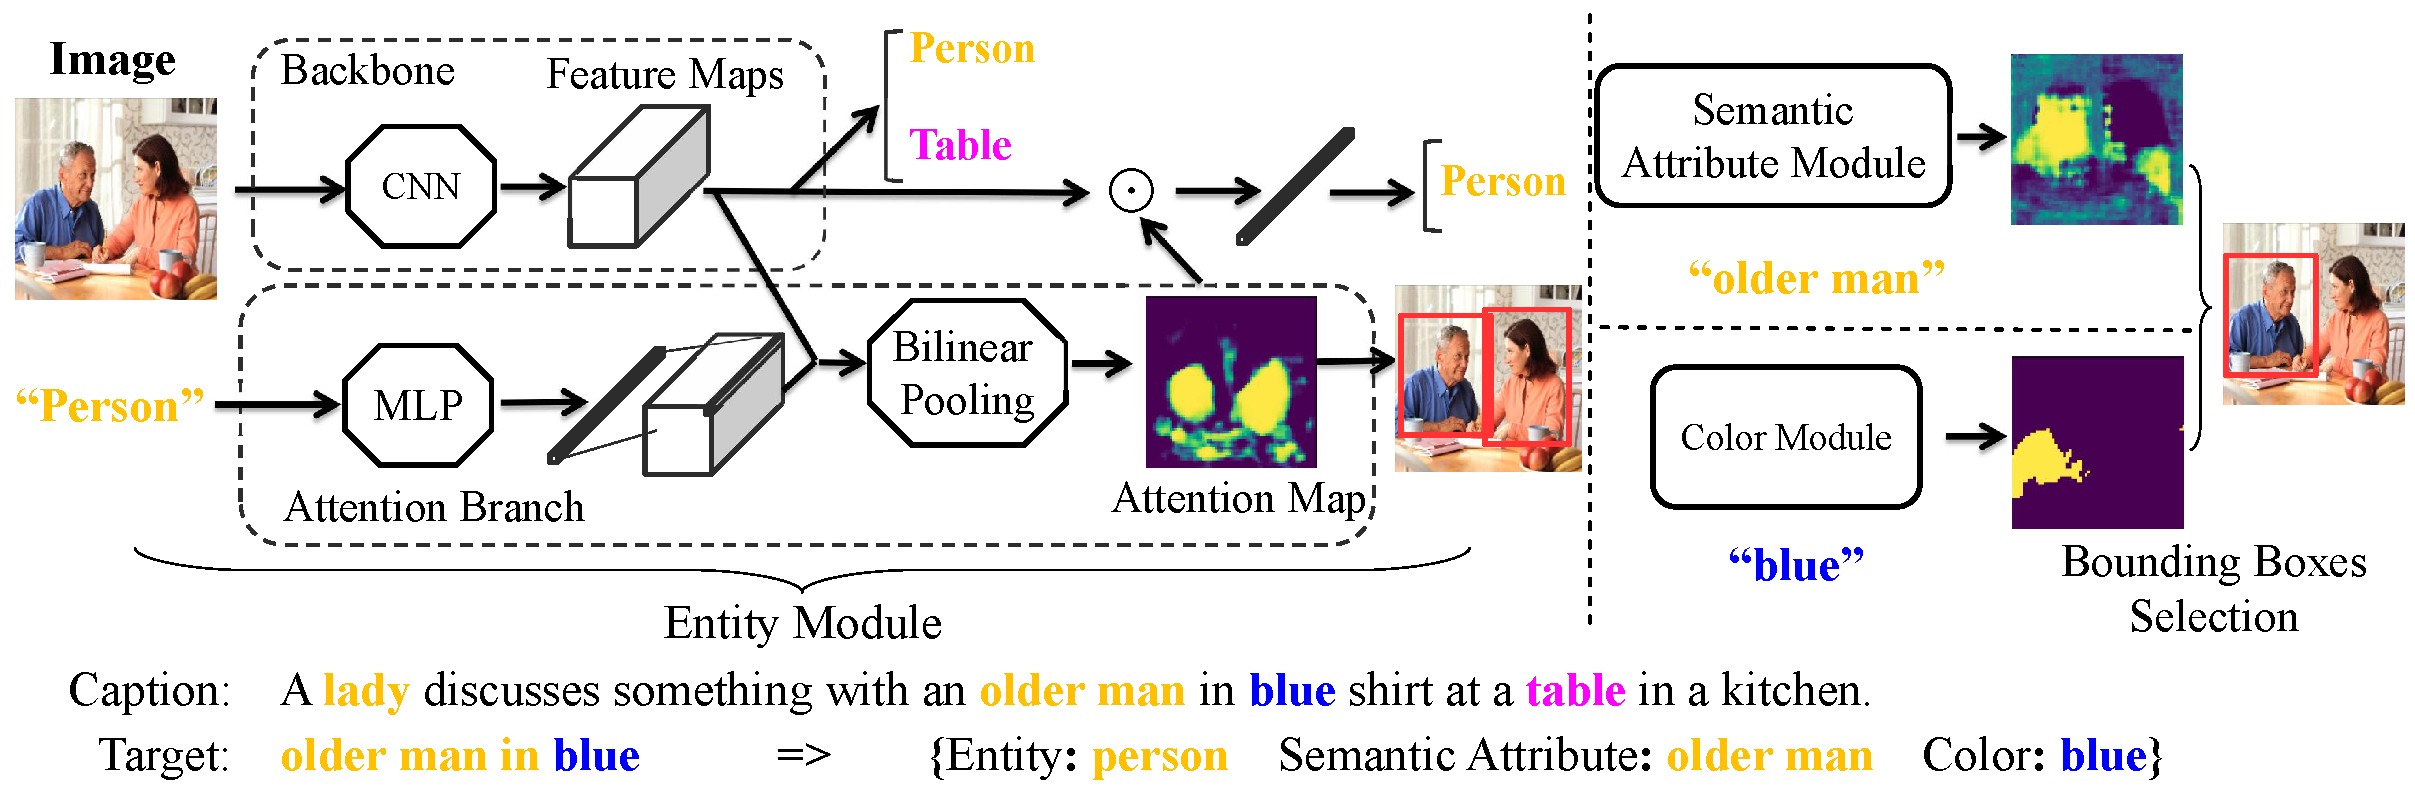
\includegraphics[width=1.0\linewidth]{images/pipeline.pdf}
\end{center}
\caption[Illustrative diagram for our entity grounding module (left) and the whole
textual grounding system(right).]{Illustrative diagram for our entity grounding module (left) and the whole
textual grounding system (right). The textual phrase is first decomposed into sub-elements, e.g., ``older man in blue" can be parsed to ``person'' category with ``older man'' and ``blue'' to be it's attributes, and later fed into corresponding sub-module. The bounding boxes are generated and selected based upon the merged attention maps. We train the entity/semantic attribute grounding module in a weakly supervised fashion with a attention mechanism. The semantic attribute module also adopt similar architecture of entity module, however with a dictionary learning loss. (best viewed in color)}
\label{fig:pipeline}
\end{figure*}


To overcome the limitation of current methods that require expensive manual annotations at fine-grained level,
we propose to train the entity grounding module in a weakly supervised learning manner.
This can help our system achieve better generalizability to other novel data domains which may just require fine-tuning over dataset annotated coarsely at image level.
This weakly supervised learning can be expressed as selecting the best region $r$ in an image $I$ given an object of interest represented by a textual feature $t$, e.g., a word2vec feature.
With well pre-trained feature extractor, we first extract visual feature maps $v$ over the image, 
based on which we train an attention branch $F$ that outputs
a heatmap expected to highlight a matched region in the image. 

Mathematically, we are interested in obtaining the region $R = F(t, v)$ in the format of heatmap and making sense of it. In practice, we find training a classification model at image level with the attention mechanism works well for entity grounding, which is the output through the attention maps, as illustrated by Figure~\ref{fig:pipeline} left. Moreover, rather than using a multiplicative gating layer to make use of the attention map, we find that it works better by using a bilinear pooling layer \citep{lin2015bilinear,gao2016compact,kong2017low}.

For bilinear pooling, we adopt the Multimodal Compact Bilinear (MCB) pooling introduced in~\citep{fukui2016multimodal} that effectively pools over visual and textual features. In MCB, the Count Sketch projection function \citep{charikar2002finding} $\Psi$ is applied on the outer product of the visual feature $v$ and an array repeating the word feature $t$ for dimensionality reduction: $\Psi (t)\ast \Psi(v)$. If converted to frequency domain, the concatenated outer product can be written as: $\Phi= {FFT}^{-1}(FFT(\Psi (t))\odot FFT(\Psi(v)))$. Based on $\Phi$, the final 2D attentive map $R$ is computed through several nonlinear 1$\times$1 convolutional layers : $R$ = $conv(\Psi)$, with the final one as sigmoid function to shrink all values into $[0,1]$. Later we retrieve the regional representation $f$ by a global pooling over the element wise product between entity attentive map and original visual feature maps: $f = pool(R\odot v)$, on which the weakly supervised classification loss is applied.
Overall, to train the entity grounding module with the attention mechanism in a weakly supervised learning fashion,
we train for image-level $K$-way classification using a cross-entropy loss.



\subsubsection{Semantic Attribute Grounding Module (M$_{a}$)}
The semantic attribute grounding module improves interpretability of the whole textual
grounding system by explaining that it explains how the final decision is being made. For example, a model finding the ``man in black suits'' as shown in Figure~\ref{fig:ca_demo} should not only output the final grounding mask, but also explain how the final result is being achieved by showing where ``man'' and ``black suits'' are localized in the image.

We also train this module with a weakly supervised learning protocol with similar architecture in the entity module.
But instead of training with $K$-way classification over $K$ predefined attributes as in training entity grounding module, we model this as a multi-label problem, since an image may deliver multiple attributes which are not exclusive to each other. Moreover, rather than classifying them, we propose to use regression for training, since attributes can become large in number while the features representing attribute names can lie in a manifold in the semantic space. This makes our module extensible to more novel attributes even trained with some pre-defined ones.

Note that we represent each attribute with the word2vec feature \citep{mikolov2013distributed}.
Although the word2vec model demonstrates very semantic grouping on words,
we find that these features representing attributes do not deliver reasonable discriminativeness. For example, in word2vec features,
``man'' is more similar to ``woman'' than ``boy'' but we care more about the gender meaning in practice.
Though retraining such a word2vec model solves the problem,
we adopt an alternative method in this paper by proposing a dictionary based scoring function
over the original word2vec features.
We note that this method not only offers more discriminative scoring power,
but also inherits the semantic manifolds in word2vec features,
extensible to novel attributes without re-training whole model as done in $K$-way classification.

To introduce our dictionary based scoring function,
we revisit the classic logistic normalization widely used in binary classification as below:

\begin{equation}
	y_i = \frac{1}{1+\exp(-\w_i^T\x)}
\end{equation}

where ${\bf w}_i$ here represents the learning parameters, 
and ${\bf x}, y_i$ are the input vectors and predicted probability with respect to class $i$.
Note again that, although the logistic loss works well for binary classification
or multi-label classification,
it is not extensible to novel classes unless retraining the whole model.
Our solution to this is based on the proposed dictionary based scoring function.
Suppose there are $C$ attributes, represented by word2vec and stacked as a dictionary
${\bf D}=[{\bf d}_1, \dots, {\bf d}_C]$.
We can measure the (inverse) Euclidean distance between $\x$ and each dictionary atom
for the similarity about which attribute $\x$ is predicted.

So the dictionary acts as the parameter bank
which can be fixed if we want to preserve the
semantic manifold in the word2vec feature space,
and we have the following modified sigmoid transformation:
\begin{equation}
	y_i = \frac{2}{1+\exp(\Vert{\bf d}_i-\x\Vert_2^2)}	
\end{equation}
However, as this may also be less discriminative,
we opt to learn a new latent space.
Concretely, we build new layers before the sigmoid transformation,
and these layers form new function $\phi$ and $\psi$
to transform the feature $\x$ and dictionary atoms, respectively.
Then we have the following dictionary based scoring function for the $i^{th}$ attribute:
\begin{equation}
	y_i = \frac{2}{1+\exp(\Vert \psi({\bf D})_i - \phi(\x)\Vert_2^2)}	
\end{equation}


Furthermore,
despite using the dictionary based scoring function as a modified sigmoid for logistic loss over
the holistic feature globally pooled over the image,
we also perform it at pixel levels.     % as in~\citep{kong2018recurrent}.
Concretely,
during each iteration on each training image,
we choose the $T$ pixels with the top scores to feed into the logistic loss.
This practice is essentially a multi-instance learning at pixel level ~\citep{paul2018w}.
We find in our experiment that jointly using the two losses helps generate
better attention maps.



\subsubsection{Color Grounding Module (M$_{c}$)}
When querying in natural languages,
human beings typically rely on textual descriptions for low-level vision characteristics,
e.g., color, texture, shape and locations.
Recent work also demonstrates the feasibility of grounding low-level features in unsupervised learning~\citep{vondrick2018tracking}.
In our work for the datasets we studied in our work,
we notice that color is the most used one.
In the Flickr30k Entities dataset~\citep{plummer2015flickr30k} as studied in this paper, 
70\% attributes words are colors describing persons. 
Therefore, 
without loss of generalization, 
we propose to build a separate color grounding module to
improve the interpretability of the whole textual grounding system.


Different from entity grounding and semantic attribute grounding modules,
we train this color grounding module in a fully supervised way over a small-scale dataset, called Color Name Dataset~\citep{van2007learning},
which contains 400 images with color name annotations at pixel level.
We essentially perform pixel-level color segmentation over the input image
to ground color reference. Moreover, we build this color grounding module over a ResNet50 model~\citep{he2016deep} pretrained on ImageNet dataset~\citep{deng2009imagenet}, and concatenate intermediate features at lower levels for pixel-level color segmentation. We find this works better than combining high-level features. We conjecture the reason is due to that color is a very low-level cue that does not require deep architectures and high-level feature abstraction. This is consistent with what reported in \citep{larsson2016learning}.





\begin{figure*}[t]
\begin{center}
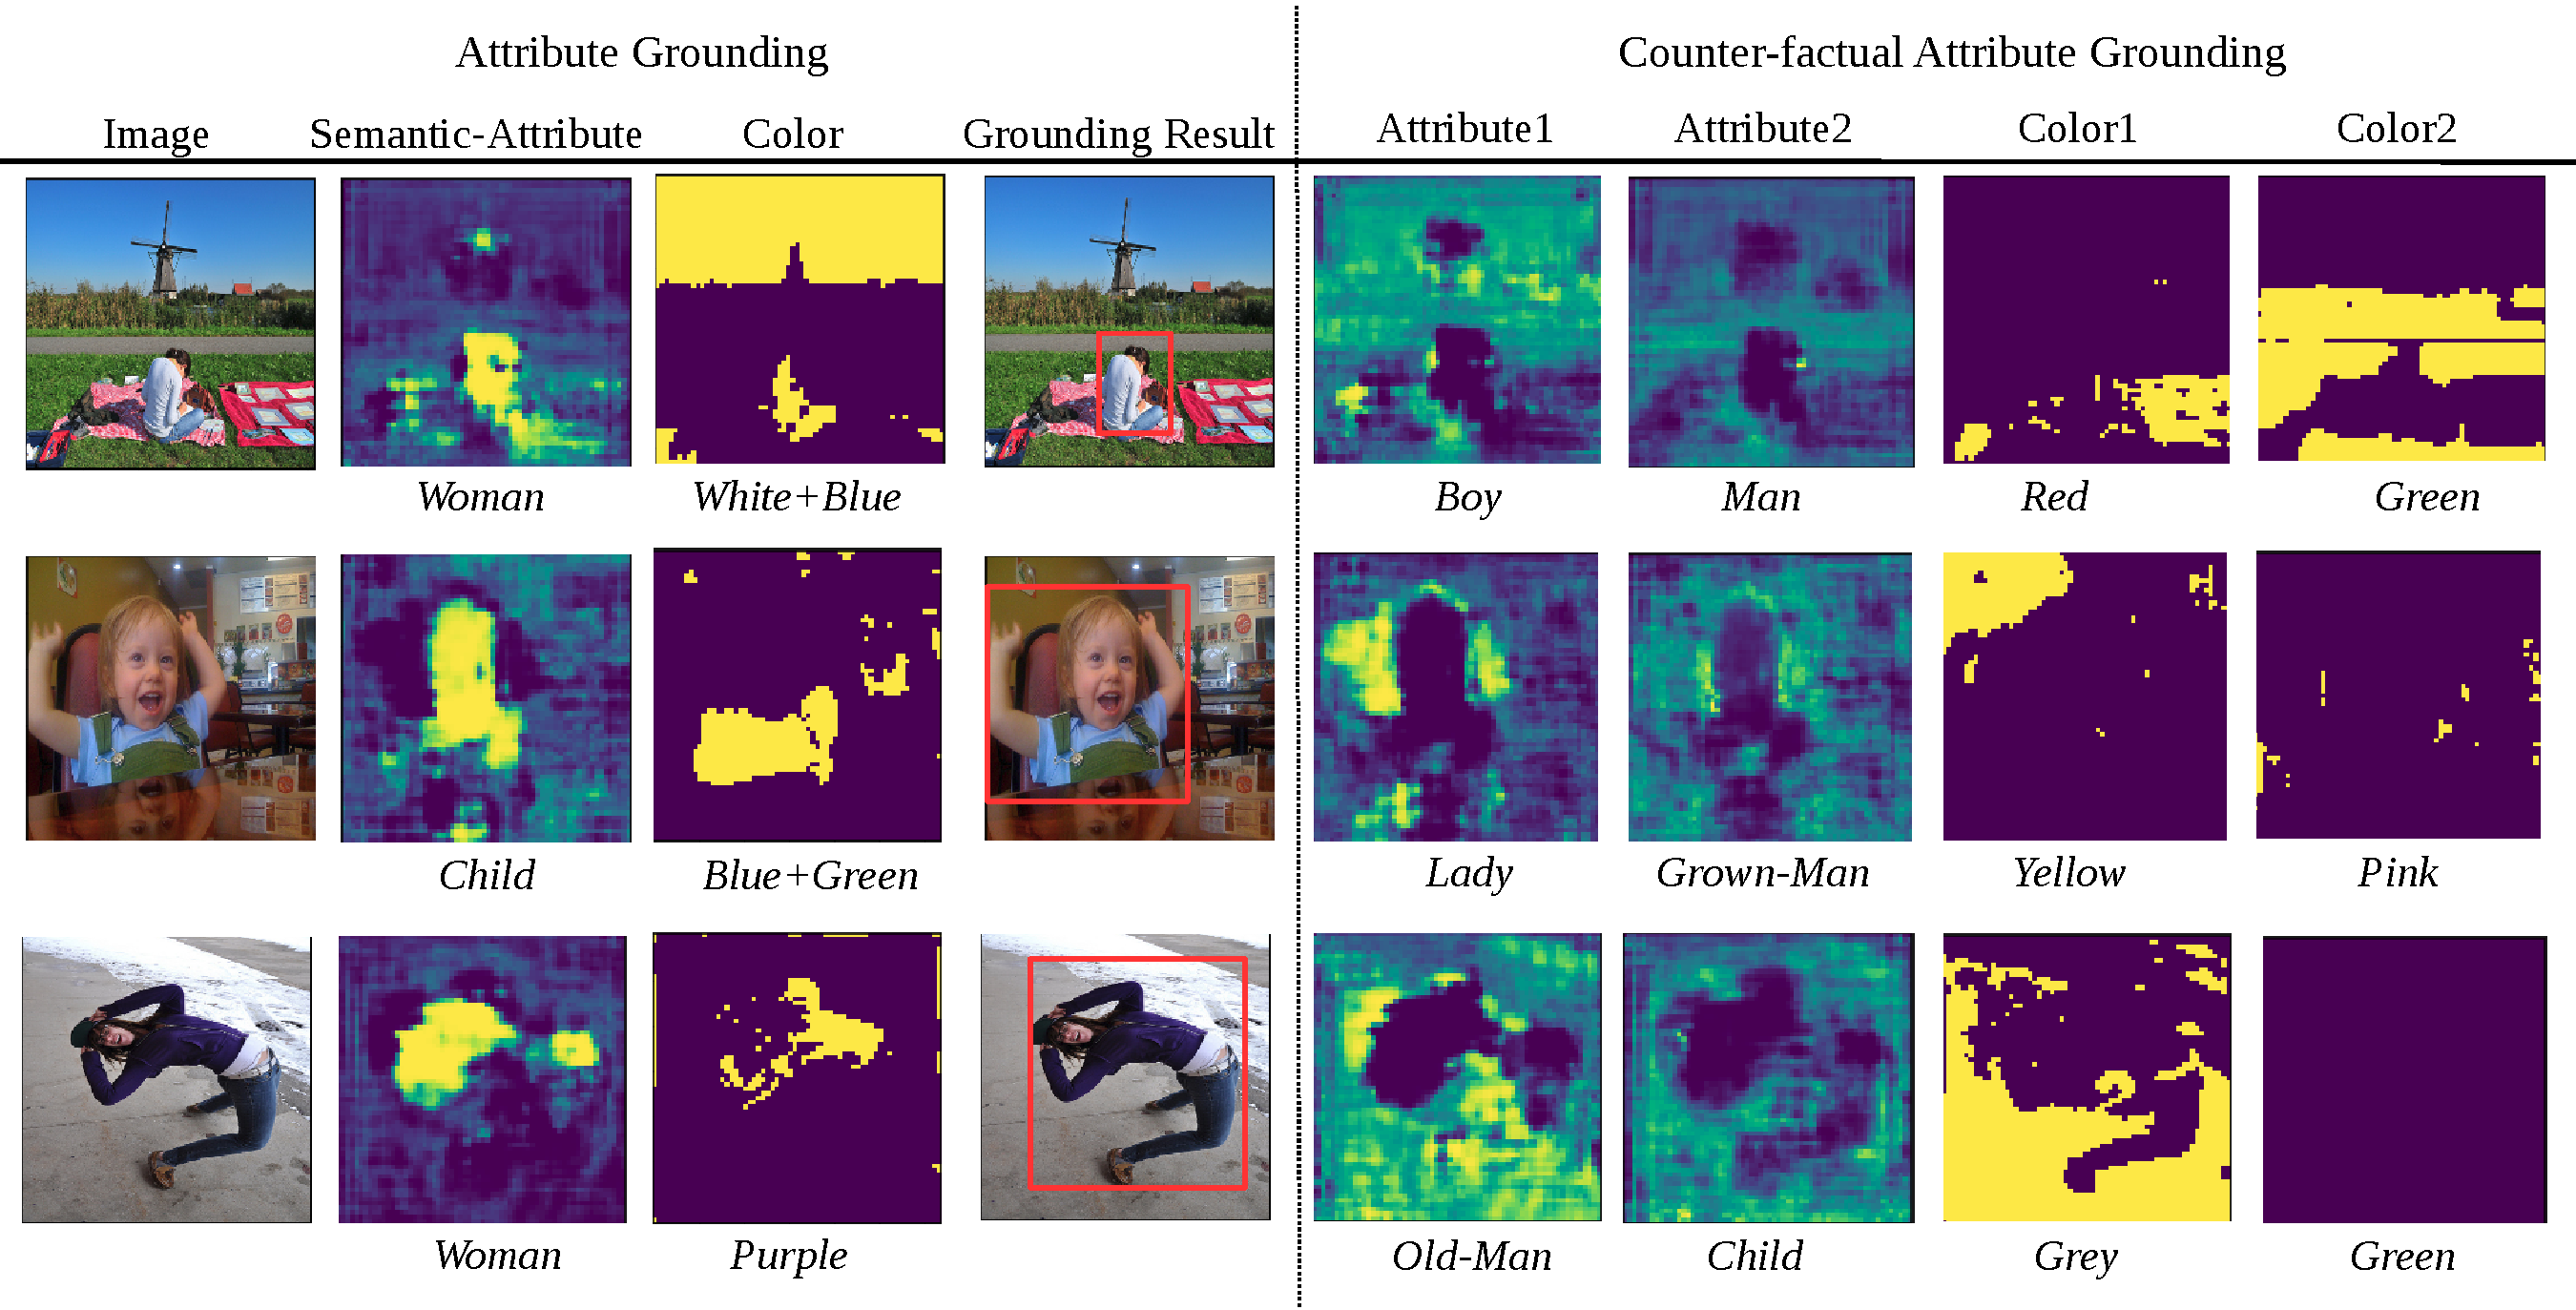
\includegraphics[width=1.0\linewidth]{images/qualitative.pdf}
\end{center}
\caption{Examples of attribute grounding predictions (left) and counterfactual attribute grounding results (right). (best viewed in color) }
\label{fig:demo}
\end{figure*}



\subsubsection{Architecture and Training}
Our three modules are based on the ResNet architecture~\citep{he2016deep}.
Similar to~\citep{chen2018deeplab,kong2017recurrent}, we increase the output resolution of ResNet
by removing the top global $7\times 7$ pooling layer and the last two $2\times2$
pooling layers, replacing them with atrous convolution with dilation rate 2 and
4, respectively to maintain a spatial sampling rate.
Our model thus outputs
predictions at $1/8$ the input resolution which are upsampled for benchmarking.
For (multi-label or $K$-way) classification,
we use a global pooling layer that produces a holistic image feature for classification.
In addition, we also insert an $L_{2}$ regularization over the attention maps,
and we observe that such a regularization term helps reduce noises effectively.

We use the standard stochastic gradient decent (SGD) for training in a stagewise fashion.
Specifically,
we first train a plain classification model for entity and semantic attribute grounding modules,
then we build the attention branch for attentional learning.


Though our textual grounding system is end-to-end trainable,
we train each module separately.
And though joint training is straightforward to implement,
we do not do this for practical reasons:
1) we can easily plug in a better trained module without retraining the whole system
for better comparison; 2) we focus on the modular design,
isolating the influence of the settings and parameters of each module.


\begin{figure}[h]
\begin{center}
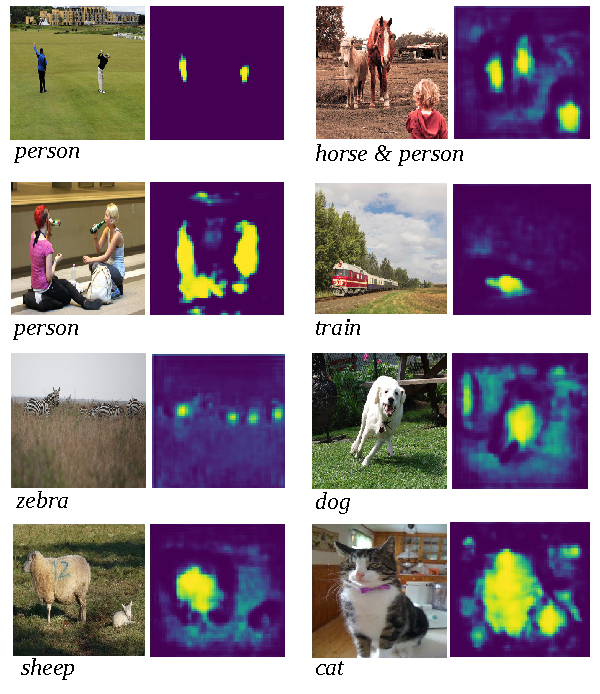
\includegraphics[width=.95\linewidth]{images/entity_demo.pdf}
\end{center}
\vspace{-7mm}
\caption{Qualitative examples of attention maps from the entity module.  }
\vspace{-5mm}
\label{fig:entity_demo}
\end{figure}


\subsection{Experiment}
We now experimentally validate our system and compare it with the state-of-the-art methods.
To highlight the generalizability of our system,
we train it on COCO2017 dataset~\citep{lin2014microsoft}
while test it on another Flickr30K Entities dataset~\citep{plummer2015flickr30k}.
We first introduce the two datasets briefly before conducting thorough comparisons,
then we carry out another experiment to show our (weakly supervised) model performs remarkably better than other (fully supervised) methods on a collected dataset consisting of counterfactual testing cases.


\subsubsection{Datasets and Preprocessing}
The two datasets we used in our experiments are:
COCO2017~\citep{lin2014microsoft} for training our system
and Flickr30k Entities Dataset \citep{plummer2015flickr30k} for testing it.

COCO2017 dataset contains 110k training images with 80 object categories at image level.
These 80 object categories are used for training our entity grounding module as they can be
seen exclusive to each other.
The captioning task and the annotations provided in COCO2017 enables us to train
our semantic attribute grounding module. Using \citep{bird2009natural,miller1998wordnet}, we tokenize and mine out words related to semantic attributes
(e.g., man, woman, boy, old and young) to form our corpus.
To train the semantic attribute grounding module,
we retrieve images from COCO2017 whose captions contain the attributes existing in our corpus.
Eventually,
10,000 images and 34 attributes are collected from COCO2017 for weakly supervised training our modules.
To alleviate imbalanced distribution of these attributes,
we adopt inverse frequency reweighting during training.

The Flickr30k Entities dataset contains over 31k images with 275k bounding boxes with natural languages descriptions,
and we only use this dataset for testing our system with the bounding boxes.

To carry out counterfactual testing experiment,
we collect a new testing set with images from Flickr30k and RefCOCO+ \citep{kazemzadeh2014referitgame}.
The images only contain persons and relevant attributes (e.g., gender, age, etc),
so we call this dataset Person Attribute Counterfactual Grounding dataset (PACG).
By developing an easy-to-use interface,
we are able to generate counterfactual captions for a given image with the good captions provided by the original dataset. Similar to work in \citep{hendricks2018generating}, we generate counterfactual attributes by mining the negation of existing attributes. The overall PACG dataset consists 2,000 images,
a half of which are with counterfactual attributes not existing in the image
and the other half with ``correct'' attributes.


\noindent{\bf Language Processing:}
To deal with free-form textual queries,
we use a language parser ~\citep{bird2009natural} to select the keywords according to the functionalities of the three modules.
We first extract the entity words and pick the most similar object classes by word similarities.
We then extract the semantic attribute words in the same way.
Finally, we extract the the color keywords simply for the color grounding.
%Furthermore, according to the word frequence statistics on Flickr 30k \citep{plummer2015flickr30k}, 70\% of the remaining semantic attribute words are related to person and colors. Thus we restricted our semantic dictionary to only human-related visual properties together with color informations. We pick  25 human-related attributes words that mainly cover the gender and age attributes.
To represent the textual attributes and color names,
we adopt the word vectors from GloVe \citep{pennington2014glove}.
This enables meaningful similarity between the defined attributes/colors and
novel ones when encountered at testing stage.
%\TODO{When constructing semantic attribute dictionary, we refer to the WordNet~\citep{miller1998wordnet} and compute word to attribute similarities among each word-attribute pairs.}%




\newcommand\Tstrut{\rule{0pt}{2.2ex}}        
\newcommand\Bstrut{\rule[1.6ex]{0pt}{0pt}} 

\begin{table}[htbp]
\begin{center}
\caption{Phrase localization performance on Flickr 30k Entities (accuracy
in \%). }
\begin{tabular}{c c c}
\toprule
Aprroach & Image Features & mAP (\%)\\
\hline
\textbf{Supervised} \Tstrut\\
SCRC \citep{hu2016natural} & VGG-cls & 27.80\\
GroundeR$_{s}$ \citep{rohrbach2016grounding} & VGG-cls & 47.81\\
CCA \citep{plummer2015flickr30k} &  VGG-det & 50.89\\
IGOP \citep{yeh2017interpretable} &  YOLO+DeepLab & \textbf{53.97}\\
\hline
\textbf{Unsupervised} \Tstrut\\
Largest proposal & n/a &  24.34\\
GroundeR$_{u}$ \citep{rohrbach2016grounding} & VGG-det & 28.94\\
Mutual Info. \citep{zitnick2013learning} & VGG-det & 31.19\\
UTG \citep{yeh2018unsupervised} & VGG-det & 35.90\\
UTG \citep{yeh2018unsupervised} & YOLO-det & 36.93\\
\hline
\textbf{Weakly-Supervised}\Tstrut\\
Ours$^{1}$  & Res101&  29.01\Tstrut\\
Ours(Attr)   & Res101& 32.04\\
Ours(Attr+Col)  & Res101& 33.43\\
Faster-RCNN~\citep{ren2015faster} & Res101-det& 35.35\\
Ours+Attr   & Res101-det& 47.46\\
Ours+Attr+Col  & Res101-det& \textbf{48.66}\\
\bottomrule
\end{tabular}
\end{center}
\label{table:flickr}
\end{table}



\subsection{Result}
We compare our modular textual grounding system with
other supervised/unsupervised methods on the Flickr30k Entities dataset.
We use the mean average precision (mAP) metric to measure the quantitative performance.
The detailed comparison is listed in Table~\ref{table:flickr}.

As the first baseline method similar to~\citep{yeh2018unsupervised},
we select the largest proposal as the final result.
This method achieves 24.34\% mAP.
Then, we build another baseline model that
we train the entity grounding module only through weakly supervised learning over a ResNet101 backbone, which is pretrained over ImageNet dataset. Then, over the entity grounding heatmaps,
we generate bounding boxes candidates by sub-window search \citep{lampert2009efficient} together with contour detection results, followed by a Non-Maximum Suppression to further refine the proposal boxes. We select the box that encompasses largest ratio of object according to equation \ref{eq:att}. We note that this simple baseline module (29.01\% mAP) outperforms GroundR$_{u}$~\citep{rohrbach2016grounding} (28.94\% mAP) that learns grounding in an attentive way over large-scale training data.
If we include our semantic attribute module,
we improve the performance further (32.04\% mPA),
outperforming Mutual Info.~\citep{zitnick2013learning}. If we further insert the color grounding module,
we achieve comparable performance (33.43\%) to UTG (36.93\% mAP),
which adopts an unsupervised method to link image concepts to query words~\citep{yeh2018unsupervised}.
We note that our models are trained on COCO dataset only,
unlike all these methods which are trained on the same dataset (Flickr30k dataset).
The effectiveness of our model is demonstrated by its good transferability, as it is trained and tested
on different data domains.


\begin{figure}[t]
\begin{center}
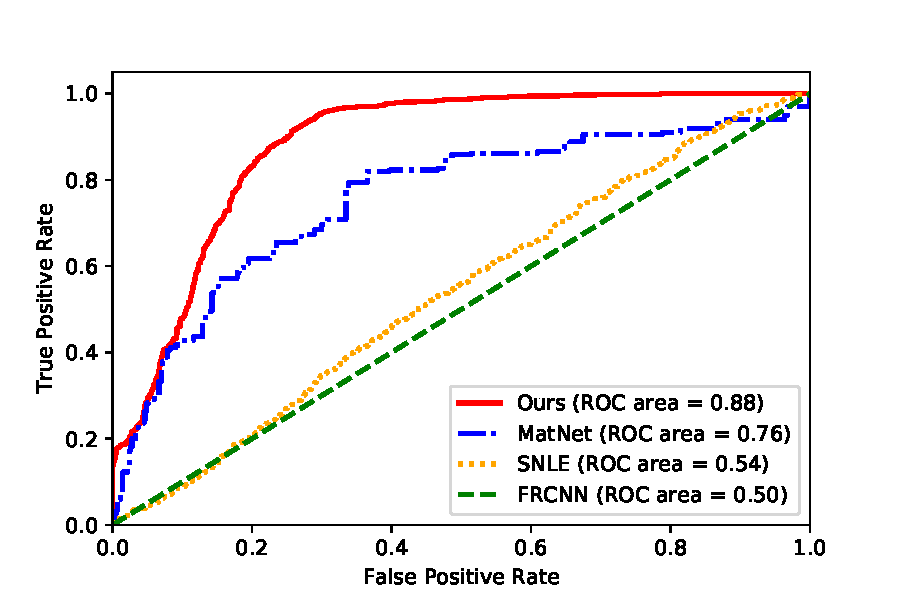
\includegraphics[width=1.1\linewidth]{images/roc}
\end{center}
\caption{ROC of our modular network demonstrates high resolving ability on PACG dataset with an AUC of 0.88, comparing to other state of the art baseline models (best viewed in color).  }
\label{fig:roc}
\end{figure}

It is also worth noting that, all the compared unsupervised methods unanimously adopt a well-trained object detector, even though they claim to be unsupervised learning.
To gain an idea how the detector improves the performance,
we fine-tune the faster-RCNN detector~\citep{girshick2015fast} on COCO
and train our modules with weak supervision again.
We report our results as the bottom two rows in Table \ref{table:flickr}.
Now we can see our models perform significantly better, and even surpasses some fully supervised methods (SCRC~\citep{hu2016natural}
and GroundeR~\citep{rohrbach2016grounding}).
Although it seems unfair that our system adopts ResNet101 architecture
while most compared methods uses shallower VGG networks,
we note that IGOP which adopts both VGG and ResNet101 (denoted by DeepLab) 
achieves the best performance with fully supervised training.
Even though our best model does not outperform IGOP,
we believe the performance gap is small and reasonable as our training is carried out
on a different dataset (COCO) rather than Flickr30k, and it does not
rely on any strong supervision signals. We show output examples of entity grounding module in Figure \ref{fig:entity_demo} with various object categories as input, and attribute grounding outputs in Figure \ref{fig:demo}, with both existing attributes and counterfactual attributes as queries. These visualizations demonstrates how our system rejects  in an explainable way the counterfactual queries through the modular output.

\subsubsection{Counterfactual Grounding Evaluation}
We now carry out in-depth study on how our system performs when facing of counterfactual textual queries over our collected
PACG dataset, and compare with three baseline or state-of-the-art methods, Faster-RCNN~\citep{ren2015faster}, MattNet \citep{yu2018mattnet}, SNLE \citep{hu2016segmentation}. We plot the ROC curves for these methods in Figure~\ref{fig:roc}. Textual grounding system then selects the region with highest scores/probability. We compare the prediction scores/probabilities of the predicted regions between the counterfactual queries and normal queries and expecting to observe distinct difference between their numerical scores.

We clearly see from the figure that our system achieves the highest AUC among of these methods, meaning that modular design successfully increases the counterfactual resilience of the grounding system. Specifically, end-to-end models like SNLE \citep{hu2016segmentation} encode the textual query
into a vector representation to extract spatial feature maps from the image as response map. However, such encoding do not consider the internal structure of sentences \citep{macwhinney1997second}, also neglecting semantic nuances of near-synonyms. Note that MattNet~\citep{yu2018mattnet} also adopts a modular design, but it is trained with fully supervised learning, also it is not easily extended to novel attributes and unable to reject counterfactual queries as effectively as our method.
The AUC of Faster-RCNN is approximately 0.5 since the recognition ability is restricted to entity-level and not been able to discern among semantic attributes.
We conclude that with the modular design and better scoring function in each modules, our model demonstrated highly resilient ability against counterfactual queries, even with only weakly-supervised training.


\subsection{Conclusion}
In this work, we propose to modularize the complex textual grounding system
by decomposing the textual description/query into three parts:
entity, semantic attributes and color.
Such a modular design largely improves the interpretability and counterfactual resilience of the system.
Moreover,
we propose to train the modules in a weakly supervised way,
so we merely needs image-level labels which are easy to obtain.
This largely helps alleviate the requirement of large-scale manual annotated images for training,
and for fine-tuning if transferring the system to a new data domain.
Through extensive experiments,
we show our system not only surpasses all unsupervised textual grounding methods
and some of fully supervised ones,
but also delivers strong resilience when facing counterfactual queries.

Our modularized textual grounding system is of practical significance as it can be deployed
in various problems.
We show how our system can be applied to video captioning correction and visual-textual search.
We expect more applications can benefit from our modular design.


\section{Video Moment Localization via Languages from Weak Supervisions}

Videos 
%abundant in number and usually are paired with other modalities (e.g., language captions and audios), 
contain much richer information for humans to interpret the world.
Building an intelligent system to automate video analysis could yield a wide range of applications benefiting human society at large, from assistive robots for the elderly to video surveillance for security~\citep{kim2018textual,yang2015robot,oh2011large,fang2020video2commonsense}. A significant component in such a system is to capture the association between video frames and textual reference/queries, \emph{a.k.a} temporal-textual association~\citep{gao2017tall,anne2017localizing,liu2018cross,ge2019mac}. Therefore, learning temporal-textual association over videos becomes a promising direction in the community~\citep{anne2017localizing,sun2019videobert,miech2019howto100m}.\\ One way to obtain such a model for temporal-textual association learning is to fully supervise the training over a video dataset which has meticulous annotations in term of the associated frames with some textual queries~\citep{chen2018temporally,anne2017localizing,gao2017tall,zhang2019man,ge2019mac}. However, we note that such a practice inevitably demands a large-scale  dataset, which apparently is not only prohibitively expensive to collect, but also largely limited in terms of diversity of both videos and  textual expressions. As an alternative, a few recent methods propose to learn the temporal-textual association only with weak annotations, \emph{i.e.}, video-level expressions in the form of natural language description~\citep{Mithun_2019_CVPR,lin2019weakly}.\\Though the weakly-supervised temporal-textual association learning attracted increasing attention until just recently, there exists a great number of works on related topics, such as weakly supervised action localization in videos~\citep{singh2017hide,paul2018w,mishra2018generative,nguyen2018weakly}.
However, compared to action localization which only has a limited number of action categories,
grounding textual reference is more challenging since the textual expressions 
could be more free-form with multiple words for the same meaning and flexible sentence structures.
In another word,
using the natural-language descriptions greatly
enlarges the content and diversity of visual-expression searching;
the combinatorial nature of open-form languages also makes it infeasible 
to enumerate all possible expressions towards the same indication.
%describing the video moment by just categorical labels limits these systems' applicability since the pre-defined action set might not fully capture the vast amount of diverse actions that exist in videos. 
For instance, 
instead of just localizing the video frames with categorical labels like  ``\textit{kissing}'' or ``\textit{person}'', 
a more practical and user-friendly query might be 
``\textit{the moment when the new couple are kissing in the wedding}'' (for moment retrieval) 
or ``\textit{a man in yellow shirt appearing in the hall in last night}'' (for video surveillance).
This necessitates the study of temporal grounding using natural language descriptions.
To foster the study, 
Gao \emph{et al.} augment the Charades 
dataset~\citep{sigurdsson2016hollywood} by generating complex language queries with temporal boundary annotations~\citep{gao2017tall};
Anne Hendricks \emph{et al.} collect the DiDeMo dataset with manual annotations 
on the associated video frames and natural-language descriptions~\citep{anne2017localizing}.
Both datasets for the first place enable training for language moment retrieval or temporal grounding. 

In this paper, basing on the datasets available in the literature,
we study learning temporal-textual association with 
weak supervisions, \emph{e.g.}, video-level language expressions
as shown in Fig.~\ref{fig:abstract}.
Until very recently, few works propose to weakly supervised train for temporal-textual association with language expressions.
In particular,
Mithun \emph{et al.} present the very first attempt for weakly supervised training
to localize video segment over the given textual queries~\citep{Mithun_2019_CVPR}. 
In general, weakly supervised methods of temporal-textual association learning
are facing two major challenges: 
1) the lack of precise supervision aligning video segments and textual queries,
2) highly undecidable features for the complex and open-form languages.

%In this work, we further propagate the fashion of weak supervision to the field of language localization with videos and stress upon the underlying significance of this for video understanding. We notice that very few work goes beyond weakly-supervised localization using more complex scenarios,\textit{ e.g.}, localizing phrases or free-form language sentences in videos. Mithun and Paul \etal in ~\citep{Mithun_2019_CVPR} first present to use the attention mechanism based method to locate the video segment without strong annotations. To be sure, almost all attempts will be thwarted by mainly several challenges: 1) The lack of valid supervision for precise textual-visual feature alignment temporally. 2) Noises of the textual features because of the complex and open-form nature of languages. 


 % why its hard and we nobody do this yet



To overcome these challenges, 
we propose a weakly-supervised framework with a referring attention mechanism (\textit{WSRA})
for learning temporal-textual associations on videos.
%With our WSRA, our model can be trained over videos only with their video-level textual descriptions  (see Figure~\ref{figure:abstract}). 
%We dub our system as \emph{\textbf{W}eakly-\textbf{S}upervised video analysis with \textbf{R}eferring \textbf{A}ttention} (WSRA) 
%to distinguish it from other weakly-supervised methods. 
The proposed referring attention mechanism summarizes a series of our novel components.
%More specifically, we facilitate WSRA with three general learning mechanisms in the context of weakly supervised video-language learning, where valid supervisions for discriminative learning and cross-modal association are made possible. 
The first one learns through a background modelling method to pool out 
irrelevant frames specific to the given language query. 
Building upon it, 
the second component encourages foreground features to align with the query
by discriminating itself from the background features from the first component. 
Within this component, 
we present a hard negative mining method integrated to sample irrelevant textual descriptions during learning. 
The third component exploits inter-video (dis-)similarity based on 
the multiple textual queries.
Specifically,
this forces the visual features to be close to each other from different videos,
as long as the queries convey similar meanings measured by the similarity of textual features.
%Similar ideas are explored in action classification~\citep{gao2017tall, zhou2018towards, gu2018ava}. 
%improving learning the visual features for 
%also adapt and introduce the cross video similarities learning in language grounding task, that enables the visual representations across videos to be close when samples contain identical visual activities inferred from their textual descriptions, which mostly exist in the action recognition based dataset \citep{gao2017tall, zhou2018towards, gu2018ava}. 

To summarize our  contributions:
1) We propose a unified framework (\textit{WSRA}) for weakly supervised learning temporal-textual associations with the referring attention 
mechanism,
directly applicable to moment retrieval and language grounding in videos.
2) We show with rigorous ablation study that the proposed components 
in the referring attention leverages better informative cues from  the limited weak supervision.
3) We justify the \textit{WSRA} through extensive experiments,
notably outperforming other state-of-the-art weakly-supervised methods on these
tasks on two public benchmarks, 
DiDeMo \citep{anne2017localizing} and 
Charades-STA \citep{gao2017tall}.

%-------------------------------------------------------------------------
\subsection{Temporal-Textual Association Learning}
The well learned temporal-textual associations on videos can allow for practical tasks like moment retrieval and temporal grounding of natural-language descriptions, where the core to it is to learn a joint embedding space for both the frames and the textual queries.
In this embedding space, the associated frames and the textual queries should be close to each other represented by the visual feature and language feature, respectively.
Formally, given a long and untrimmed video ${\cal V}=[\boldsymbol{v}_1, ..., \boldsymbol{v}_T]$ consisting of $T$ snippets of frames, and an open-form textual sentence $\boldsymbol{t}$, we would like to train a model to localize a video segment $\boldsymbol{v}_t$ from ${\cal V}$ that best corresponds to the description, which is ideally the true (yet unknown) video segment for the textual query.
We denote by $\boldsymbol{v}_t \in\mathbb{R}^{d}$ the feature vector 
extracted from a video model (\emph{e.g.}, a pretrained classification network),
and by $\boldsymbol{t}\in\mathbb{R}^{d}$ the textual feature representation of the 
query (short phrase or a sentence) from a language model.
In practice, segment features can also be the averagely pooled proposal visual features, where each proposal contains several continuous segments with various lengths. 
As weak supervision causes ambiguities in predicting the association between frames and the textual query, we present our weakly-supervised approach with the proposed referring attention mechanism (\textit{WSRA}) in this section.
Fig.~\ref{figure:over_arch} shows the overall architecture.

\begin{figure}[t]
\centering
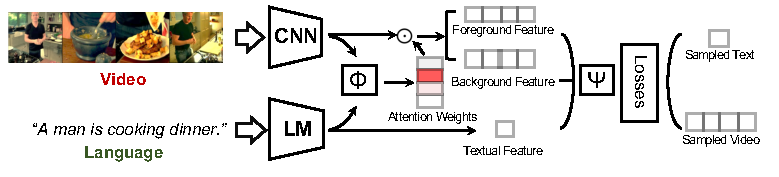
\includegraphics[width=.95\textwidth]{images/wsra_architecture.pdf}
\caption[Flowchart of the proposed \textit{WSRA}.]{\small Flowchart of the proposed \textit{WSRA}.
The losses are only used during training for temporal-textual association learning,
while inference shares the same computation flow 
for grounding textual queries over the given video. ``\textit{CNN}'' and ``\textit{LM}'' denote
video model and language model to extract features for frames and the textual query.
respectively. 
}
\label{figure:over_arch}
\end{figure}

\begin{figure*}[t]
\centering
\includegraphics[width=.95\textwidth]{images/wsra_pipeline.pdf}
\caption[ The \textit{WSRA} framework's learning losses.]{\small The \textit{WSRA} framework contains three learning losses. (a) Fore/background modelling loss forces the fore/background visual features to be discriminative by training 
over the same video \textit{w.r.t.} the ground-truth referring text $\mathbf{t}_\textit{$+$}$. (b) Video-to-text loss samples negative textual queries $\mathbf{t}_\textit{$-$}$ for each video segment for discriminative learning. The third loss is shown separately in Fig.~\ref{figure:crossvideo}.
}
\label{figure:architecture}
\end{figure*}

\subsubsection{Video-level Attention Modeling}
Prior weakly supervised methods for action localization propose to generate a weight vector to localize action labels among the video snippets in a \textit{bottom-up} manner~\citep{paul2018w,nguyen2019weakly}. While being successful in action localization from predefined categorical labels, these bottom-up methods cannot be directly tailored to the more natural language localization problem in question, as a video can correspond to multiple textual queries which appear in a very open-form language structure. Based on the fact that, the description of textual query usually covers multiple snippets in a video, we propose to model the video-level back/fore-ground features that are (ir)related to the textual query with the designed referring weights:
\begin{equation}
\begin{split}
    \boldsymbol{v}_f = &\sum^{T}_{t=1}\alpha_t\boldsymbol{v}_t \\
    \boldsymbol{v}_b = \frac{1}{T-1} &\sum^{T}_{t=1}(1-\alpha_t)\boldsymbol{v}_t,
\end{split}
\label{eq:foreback}
\end{equation}
where $v_f$ and $v_b$ are the synthesized fore/back-ground features, and weight $\alpha_t$ is calculated as:
\begin{equation}
    \alpha_t = \frac{\text{exp}(\phi(\boldsymbol{v}_t, \boldsymbol{t}))}{{\sum_{i=1}^{T}\text{exp}(\phi(\boldsymbol{v}_i, \boldsymbol{t}))}}.
    \label{eq:videoweight}
\end{equation}
In Eq.~\ref{eq:videoweight}, $\phi(\cdot, \cdot)$ is the cross-modal scoring function that measuring the distance between a frame/snippet and the textual query in the embedding space.
In practice, we define $\phi(\boldsymbol{v}, \boldsymbol{t})=\text{Sigmoid}(\text{FC}(\text{Cat}(\boldsymbol{v}, \boldsymbol{t}))$ with learnable parameters, which has a stronger association ability than cosine similarity~\citep{yu2018mattnet}, bilinear pooling~\citep{gao2016compact,fang2018modularizedtextual,kong2017low}, and second-order polynomial feature fusion~\citep{scikit-learn,gao2017tall}.
It is worth noting that the scoring function not only conveys the idea of metric learning, 
but also lands for embedding learning along with further loss terms as presented in next subsections.

As we would like to learn an embedding space in which,
1) foreground visual features tightly correspond to the given textual query measured by
the scoring function performing in the same space;
and 2) background features are clearly far away from both the foreground and textual query, as illustrated in Fig.~\ref{figure:architecture} (a).
To this end, refer to the Triplet Loss~\citep{7298682}, we set $(\phi(\boldsymbol{v}_b, \boldsymbol{t})-\phi(\boldsymbol{v}_f, \boldsymbol{t}))>m$ as our optimization target for video-level metric learning.
Rather than simply leveraging the margin or triplet-loss based contrastive learning objectiveness, we refer to the recently proposed general pair weighting framework that origins from deep metric learning~\citep{wang2020vitaa,wang2019multi}, which endows our learning objectiveness with the ability of gradient weighting using the logistic-loss as the basic form function. Comparing to the previous works as in~\citep{Mithun_2019_CVPR, chen2020look}, WSRA adaptively assigns proper weights to valuable learning pairs thus benefiting the training. 
We denote fore/back-ground similarity scores as $s_p^i=\phi(\boldsymbol{v}_f^i, \boldsymbol{t}^i)$ and $s_n^i=\phi(\boldsymbol{v}_b^i, \boldsymbol{t}^i)$, respectively. Our video-level loss function is calculated by:
\begin{equation}
    \mathcal{L}_{video} = \log\Big[1+\sum_{i=1}^{N}\exp(\gamma(s_n^i-s_p^i+m))\Big],
    \label{eq:video}
\end{equation}
in which $i$ indices the sample in a random mini-batch, $m$ is a predefined margin and $\gamma$ is a temperature factor.


\subsubsection{Snippet-level Attention Modeling}
While the above video-level loss imposed on a whole video encourages learning a discriminative embedding space and the metric functions, we introduce snippet-level modeling to enhance the contrastive study of individual video snippet and multiple textual queries, as illustrated in Fig.~\ref{figure:architecture} (b). Under this case, for the $t$-th snippet in the $j$-th video $\boldsymbol{v}_t^j$ , we calculate the referring weight $\beta_t^i$ as:
\begin{equation}
    \beta_t^j = \frac{\text{exp}(\phi(\boldsymbol{v}_t^j, \boldsymbol{t_t}))}{{\sum_{i=1}^{N}\text{exp}(\phi(\boldsymbol{v}_t^j, \boldsymbol{t_i}))}}.
    \label{eq:snippetweight}
\end{equation}



As noted, sampling semantically similar queries affect learning~\citep{wu2018unsupervised}, but when the batch size grows with limited number of textual expressions, a single training batch may contain semantically similar queries more easily,\emph{e.g.}, ``\textit{a man having food}'' and ``\textit{the man eating dinner}''. 
As a result, simply treating all other textual queries within the mini-batch as the negative samples hurt discriminative learning.
We provide our solution as below on using the similarity $(\boldsymbol{t}^i, \boldsymbol{t}^j)$ to differentiate individual instances (queries within a single
training batch), telling whether a pair of them are semantically dissimilar enough
to support a sampled negative query.




\begin{figure*}[t]
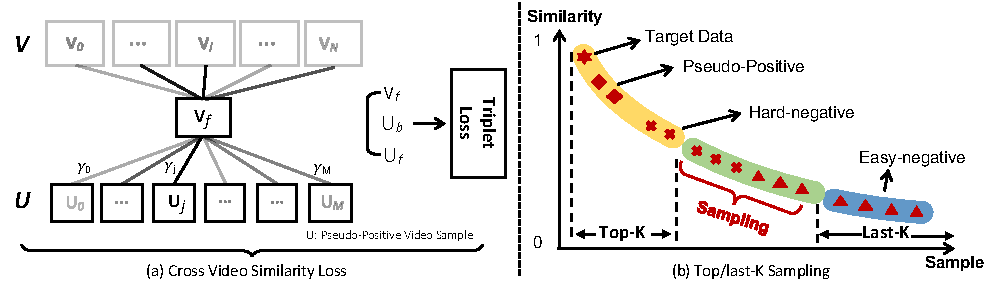
\includegraphics[width=.92\textwidth]{images/lcrov.pdf}
\centering
\caption[(a) Cross Video Similarity Loss $L_{crov}$ exploits the pseudo positive videos. (b) Demonstrative figure of queries' semantic similarity within a single training batch.]{\small (a) Cross Video Similarity Loss $L_{crov}$ exploits the pseudo positive videos, and encourage the foreground representations across samples to be similar when similar visual content occurs. (b) Demonstrative figure of queries' semantic similarity within a single training batch. The $y$-axis stands for distance measured by matching scores between
all queries and the current query in question;
$x$-axis sorts all the queries according the  matching score 
within this training batch.
%Distance represents the matching scores by computing the relevance score of the visual vector with each textual vector within the batch. 
}
\label{figure:crossvideo}
\end{figure*}
 
The negative textual queries used in the VAS loss 
are sampled within
a single training batch.
%which samples random negative textual instances within the mini-batch for the sake of learning from negative samples. 
Different with previous fore/background discriminative loss, 
VAS loss constructs a triplet as ($\boldsymbol{v}_f^i$, 
$\boldsymbol{t}^i$,
$\boldsymbol{t}^j$), 
where ($\boldsymbol{v}_f^i$, $\boldsymbol{t}^i$) are the foreground
features and corresponding (positive) textual query for the $i^{th}$ video;
and $\boldsymbol{t}^j$ is the textual query coming with the $j^{th}$ video and assumed as a negative query iff satisfying 
a condition indicated by a logic value 
${\mathbb{1}}(\boldsymbol{t}^i, \boldsymbol{t}^j)$.
We have the video-level max-margin VAS loss as below:
\begin{equation}
    \mathcal{L}_{vas} = \sum_{i=1}^{N}{\mathbb{1}}(\boldsymbol{t}^i, \boldsymbol{t}^j) \cdot 
    \text{max}(\textbf{0}, m + \psi(\boldsymbol{t}^j, \boldsymbol{v}_f^i) - \psi(\boldsymbol{t}^i, \boldsymbol{v}_f^i)).
\end{equation}
%where $\boldsymbol{t}^j$ can be the sampled negative samples within a mini-batch. 
As noted, sampling semantically similar queries affect learning~\citep{wu2018unsupervised},
but when the batch size grows with limited number of textual expressions, 
a single training batch may contain semantically similar queries more 
easily,
\emph{e.g.}, ``\textit{a man having food}'' and ``\textit{the man eating dinner}''. 
As a result, 
simply treating all other textual queries within the mini-batch as the negative samples hurt training.
We provide our solution as below on how to define ${\mathbb{1}}(\boldsymbol{t}^i, \boldsymbol{t}^j)$
to differentiate individual instances (queries within a single
training batch),
telling whether a pair of them are semantically dissimilar enough
to support a sampled negative query.





\subsubsection{Top/last-$K$ Sampling.}
Inspired by the hard negative sampling techniques in metric learning~\citep{shrivastava2016training,lin2017focal,liu2016ssd,zhang2017range}, 
we propose a top/last-$K$ sampling strategy akin to semi-hard negative sampling~\citep{schroff2015facenet}. 
We identify queries as ``pseudo-positive samples'' and ``easy-negative samples'', 
as demonstrated by Fig.~\ref{figure:crossvideo},
then we select the ``hard-negative samples'',
which provide more informative gradients that help learning.
We note ``easy-negative samples'' do not contribute to better training while being included do not hurt either yet
waste wall-clock time in computation.
To identify the ``hard-negative samples'', 
we first sort all the queries in the mini-batch based on 
the similarity scores
compared to the one given for the video of interest.
Then we simply remove the top and last $K$ samples as easy positive and negative ones.
While the hyper-parameter $K$ depends on the batch size,
we set $K=3$ in our experiments and find it quite 
stable and beneficial to the training.
%let \{$s^i_1, s^i_2 ... s^i_N$\} denotes the ranked matching scores of the video $i$, \textit{w.r.t} all textual vectors within the batch. Our negative instance $\boldsymbol{t}^j_-$ is random sampled in the set after excluding samples with relevance scores at both top and last $k$ positions, \{$s^i_{k+1}, s^i_{k+2} ... s^i_{N-k}$\} (see Figure.~\ref{figure:sample}), where $k$ is a hyper-parameter during training and depended on the batch size as well.
 
\subsubsection{Instance-level VAS Loss.}
VAS loss can be thought of a video-level multi-target learning,
\emph{e.g.}, one video with multiple textual descriptions, 
as the referring attention weights are aggregated to compute global
fore/back-ground visual features during training. 
We find further imposing a discriminative loss on individual video snippet (the instance) improves learning:
    \begin{equation}
    \label{ins-vas}
    \mathcal{L}_{ins\text{-}vas} = \sum ^{N}_{i=1}\sum^{T}_{t=1}\text{max}(\mathbf{0}, m + \alpha_{t_-}\cdot\psi(\boldsymbol{t}^i_-, \boldsymbol{v}_t^i) - \alpha_{t_+}\cdot\psi(\boldsymbol{t}^i_+, \boldsymbol{v}_t^i)),
    \end{equation}
where $\alpha_{t_+}$ and $\alpha_{t_-}$ are the referring attention weights computed by Eq.~\ref{eq:videoweight} using $\boldsymbol{t}^i_+$ (the ground-truth referring text) and $\boldsymbol{t}^i_-$ (the sampled negative text), with $\boldsymbol{v}_t^i$, 
respectively. 
We note that the weights $\alpha$ actually scales the similarity scores,
in which way the loss forces embedding learning and metric learning to be more discriminative.
%In here, the referring attention weights serve as the temperature parameters, modulating the attention weights cohere with segment-level alignment. 
We carry out ablation study on the losses in the experiment section.




% \begin{figure}[t]
% \includegraphics[width=.45\textwidth]{images/cross-video.pdf}
% \centering
% \caption{\small{Our cross video loss encourages the partial visual 
% representations across videos to be similar 
% when a common latent visual activity (if can be extracted) exists in both videos.}}
% \label{figure:crossvideo}
% \end{figure}




\subsubsection{Cross Video Similarity Loss}
%Recent efforts in in weak/un-supervision shed light upon the importance to design the learning schema that learns across instances. 
Proceeding from previous efforts in un/weak-supervised video representation learning, we are inspired with the necessity to construct contrastive learning pairs across video samples.~\citep{paul2018w} proposed to encourage the videos containing identical actions to be encoded as similar features in their corresponded temporal regions.~\citep{dwibedi2019temporal} learns the frame-wise correspondence across videos and yields great representations without any strong supervision. These works all unanimously highlight that mining the common-information among samples could enormously benefit the discriminative learning. This practice also applies for our video and language tasks, where the similar visual content can be observed in different videos. For instance, the excluded pseudo-positive samples from our VAS learning might be ``\textit{a gentleman is having dinner}'', whose visual foreground should be similar with the scenario of ``\textit{man eating food in a restaurant}''. We then exploit an inter-video loss ($L_{crov}$) for further improving the discriminativeness of learning by utilizing the mined pseudo-positive samples as stated previously. Concretely, we assume that for each target video $\boldsymbol{v}$, it contains implicit common activities with its pseudo-positive sample $\boldsymbol{u}$. Now we design our learning objective to be making their foreground representations ($\boldsymbol{v}_f, \boldsymbol{u}_f$) closer and enlarging the divergence of foreground with background ($\boldsymbol{u}_b$) as is shown in Fig.~\ref{figure:crossvideo}, where $\boldsymbol{u}_f$ and $\boldsymbol{u}_b$ is computed as the soft aggregation over all segment $\boldsymbol{u}_i$ weighted by their similarity with $\boldsymbol{v}_f$: 
\begin{equation}
    \boldsymbol{u}_f = \sum_{i}^{M} \gamma_i \cdot  \boldsymbol{u}_i.
\end{equation}
Here $M$ denotes the length of $\boldsymbol{u}$, and $\gamma_i$ represents the attention weights and are normalized by the softmax function along temporal axis:
\begin{equation}
    \gamma_i = \frac{e^{\text{cos}(\boldsymbol{u}_i, \boldsymbol{v}_f)}}{\sum_{j}^{M}e^{\text{cos}(\boldsymbol{u}_j, \boldsymbol{v}_f)}}.
\end{equation}
Since the comparing targets are from the same modality, we simply use cosine similarity as measuring function.
Our overall cross-video loss then can then be expressed as:
\begin{equation}
    \mathcal{L}_{crov} = \sum_{i=1}^{N}\lambda_i\cdot
    \text{max}(\textbf{0}, m + \frac{{\boldsymbol{u}_f^i}^T \cdot \boldsymbol{v}_f^i}{||{\boldsymbol{u}_f^i}||\cdot ||\boldsymbol{v}_f^i||} - \frac{{\boldsymbol{u}_b^i}^T \cdot \boldsymbol{v}_f^i}{||\boldsymbol{u}_b^i||\cdot ||\boldsymbol{v}_f^i||}).
    \label{equation:lcrov}
\end{equation}
We also introduce a gating parameter $\lambda_i$, which acts as the masking function that blocks out the training pairs when their textual descriptions ($\boldsymbol{t}_v, \boldsymbol{t}_u$) are not similar:
\begin{equation}
      \lambda_{i} =
    \begin{cases}
      1 & \text{if } \frac{{\boldsymbol{t}_v}^{T}{\boldsymbol{t}_u}}{||\boldsymbol{t}_v||\cdot||\boldsymbol{t}_u||} > \tau\\
      0 & \text{otherwise}\\
    \end{cases},
\end{equation}
we set $\tau=0.9$ as the similarity threshold. In such a way, we can utilize the semantic information of captions to guarantee that the constructed pseudo-positive sample is correctly chosen.
% , we found that another critical while yet under-investigated supervision comes from the cross-video samples. 
%To introduce the cross-video similarity for learned feature representations, 
% To this end,
% we initialize a random dictionary 
% $\mathbf{D} = [\mathbf{d}_1, \cdots, \mathbf{d}_C ]$
% consisting of $C$ atoms,
% which supposedly correspond to $C$ latent categories that, 
% for example, 
% describe actions or activities.
% During training,
% we also update the dictionary as described at the end of this section.
% %to contain the averagely pooled textual embedding \textit{w.r.t.} each latent class. 
% With the dictionary,
% we simply compute the cosine similarity between the textual feature with the class embedding, 
% and select the highest category as the pseudo-label. 
% Ideally, 
% we anticipate the learned visual representations across two samples to be similar in the portions 
% of videos when identical latent visual activity $\mathbf{d}_C$ occurs (see Fig.~\ref{figure:crossvideo}). 
% Our cross-video loss is defined as below:
% \begin{equation}
%     \begin{split}
%     \mathcal{L}_{crov} = \sum_{i=1}^{N}\sum_{j=1}^{C}&\uplambda_{i,j}\cdot\text{max}(\mathbf{0}, \\ 
%     m + ||{\boldsymbol{v}^i_f}{\scriptstyle[\mathbf{d}_j]} - & \boldsymbol{v}_f^+{\scriptstyle[\mathbf{d}_j]}||_2
%     - ||\boldsymbol{v}^i_f{\scriptstyle[\mathbf{d}_j]} - \boldsymbol{v}_b^+{\scriptstyle[\mathbf{d}_j]}||_2),
%     \end{split}
% \end{equation}
% where the $||\cdot||_2$ represents the Euclidean distance of two vectors, 
% $\boldsymbol{v}_f^i[\mathbf{d}]$ represents the video-level foreground feature when the referring signal is latent class embedding $\mathbf{d}$, and $\lambda_{i, j}$ is the mask function that is expressed as:
% \begin{equation}
%       \uplambda_{i,j} =
%     \begin{cases}
%       1 & \text{if } \frac{{\mathbf{d}_j}^{T}{\boldsymbol{t}^{i}}}{||\mathbf{d}_j||\cdot||{\boldsymbol{t}^{i}}||} > \tau\\
%       0 & \text{otherwise}\\
%     \end{cases}
% \end{equation}
% we set $\tau=0.9$ as the similarity threshold.
% During training, 
% class dictionary $\mathbf{D}$ is updated by averaging the matched embedding: 
% $\boldsymbol{d}_i\rightarrow(\boldsymbol{d}_i+\boldsymbol{t})/2$ in each iteration. 
% It is worth noting, 
% when $C$ increases to the number of whole training samples, 
% our cross video loss is reduced to the regular instance-level learning 
% without the notion of latent classes. 
% Essentially, 
% our cross-video loss encourages the cross-video visual features  to be similar when they share similar descriptions,
% defined by the latent dictionary being updated to cluster semantically similar textual queries.
\subsection{Overall Training Loss}
As for the overall objective loss,
we combine all the above loss terms for end-to-end training our model:
\begin{equation}
    \mathcal{L} = \alpha\mathcal{L}_{bg} + \beta\mathcal{L}_{crov} 
    + \gamma\mathcal{L}_{vas} + \delta\mathcal{L}_{ins-vas} \\
    \label{eq:overall_loss}
\end{equation}
where $\alpha, \beta$, $\gamma$ and $\delta$ are hyper-parameters weighting the loss terms.
% \shu{Shouldn't we add one sentence to say we didn't tune these hyper-parameters too much, but incrementally search over grids of choices one-by-one. refer to what we wrote in the rebuttal.}
We independently study each loss weight on top of $L_{bg}$, 
then incrementally combine all the losses and train the final model.
We list details on the use of these loss terms in the ablation study for specific tasks involved in our experiments.
During training,
we use the Adam optimizer 
with constant learning rate $10^{-4}$ and coefficients 0.9 and 0.999
for computing running averages of gradient and its square.
We implement our algorithm using PyTorch toolbox~\citep{paszke2017automatic} 
on single GTX1080 Ti GPU.

\subsection{Experiment}
The goal of our experiments is to validate the effectiveness of 
the proposed weakly-supervised framework with the top-down referring attention (\textit{WSRA}) 
for temporal-textual association learning,
through two tasks of moment localization and language grounding on
the  DiDeMo~\citep{hendricks2018localizing} and Charades-STA~\citep{gao2017tall},
respectively.
We use the mean Average Precision (mAP) 
under various Intersection over Union (IoU) thresholds to measure the performance. 
First, we elaborate on some important details about the models and language features.
We then compare our \textit{WSRA} with other state-of-the-art methods with
systematical ablation studies on the two tasks over the two benchmarks.
Finally, we visualize the qualitative results produced by our \textit{WSRA}.
% \footnote{
% Code and models will be  released
% \url{https://XXX.XXX/XXX}.}
%To show the effectiveness of our learning framework, we also conduct ablation study on the combination of various loss functions. At last, we show qualitative results of our language grounding task and analyze its future study and applications.

\noindent \textbf{Language Processing and Feature Extraction}.
The proposed  \textit{WSRA} framework is agnostic to the choice of language models.
Although one is free to use any language models providing features to represent
the textual queries (\emph{e.g.}, natural-language sentence or short phrase),   
we turn to the Openai-GPT2~\citep{radford2019language}, 
which is a released language model\footnote{\url{https://github.com/openai/gpt-2}}
trained over large-scale, diverse corpus (Wikipedia, news and books). 
% Ablation study shows that language feature extractor does not obviously benefit the performance of our model as indicated by our ablation study. 
%More specifically, we use the official released large version of GPT2\footnote{\url{https://github.com/openai/gpt-2}} (774M parameters) pre-trained on diverse corpus (Wikipedia, news and books) on the task of next word prediction. 
GPT2 is composed of a stacking of repetitive transformer modules, and we retrieve our textual features by averaging all outputs from modules as done in literature~\citep{xiao2018bertservice}.

%Note that 
%We note that, since the language features are offline, 
%the use of GPT-2 as language feature extractor does not directly benefit the performance of our model as indicated by our ablation study.
%The use of pre-trained language model is only for the consideration that it provides great sentence level representations semantically, thus enabling us to cluster the latent action dictionary precisely during training.




\subsubsection{Moment Localization on DiDeMo}

For localizing moments over a given natural-language description,
we use the Distinct Describable Moments (DiDeMo) dataset~\citep{hendricks2018localizing}, 
which includes $>$10k 25-30 second long Flickr videos. 
Manual annotations contain  $>$40k sentences with temporal boundaries 
for fine localization. 
In total, the DiDeMo dataset contains 
8,395, 1,065 and 1,004 videos for training, validation and testing respectively. We report the performances of our model on the testing split and conduct ablation studies on the validation split.
As suggested by the dataset, 
to simplify association between the sentence and a video, 
each long video is divided into 6 segments, which are annotated as whether corresponding to the sentence for localization. 
In DeDeMo, each textual description is associated with only one continuous video moment, thus yielding 21 possible candidates ($\sum_{i=1}^{6}i$). 
We measure the performance using the Rank@1 (R@1) and Rank@5 (R@5) (accuracy of the top-1/5 retrieved candidates) and their mean Intersection of Unions (mIoU) when IoU=1. To extract visual features of the videos, 
we use the official provided features 
over both RGB and optical flow~\citep{anne2017localizing}. 
For fair comparisons with other methods, as done in~\citep{hendricks2018localizing,anne2017localizing}, we compute the visual features as the concatenation of the global averagely pooled features (all 21 proposal features) and the local proposal features, which are produced by after average pooling the features from each segment.
We set hyper-parameters $\delta=1$ and $\alpha=\lambda=\gamma=0.1$ in this experiment and report results under different combinations in our supplementary materials.
During inference, we select the top-5 proposals with highest attention weights as the final prediction.

% {
% \setlength{\tabcolsep}{0.3em} % for the horizontal padding
% \begin{table}[t]
% \captionsetup{font=small}
% \centering
% \caption{Ablation study of loss terms on DiDeMo and Charades-STA dataset. 
% %The results indicate our proposed joint training yields significant improvement.
% }
% \label{table:ablation_studies}
% \small
% \begin{tabular}{cccc|ccc|ccc}
% \multirow{2}{*}{$\mathcal{L}_{bg}$} & \multirow{2}{*}{$\mathcal{L}_{vas}$} & \multirow{2}{*}{$\mathcal{L}_{ins\text{-}vas}$} & \multirow{2}{*}{$\mathcal{L}_{crov}$} & \multicolumn{3}{c|}{DiDeMo} & \multicolumn{3}{c}{Charades-STA} \\
% \cline{5-10}
% % & & & & \multicolumn{3}{c}{AP@IoU}  \\
%  &  &  & & R@1 & R@5 & mIoU & R@1 & R@5 & mIoU\\
% \hline
% \checkmark & -- & -- & --  & 12.31  & 40.03  &  22.53  & & & \\
% -- & \checkmark & -- & --  & 15.77 & 47.08  &  26.80 & & &  \\
% -- & -- & \checkmark & -- & 16.92  & 48.48  & 28.67  & & &   \\
% -- & \checkmark & \checkmark & --  & 17.50  &  48.15 & 28.97 & & &  \\
% \checkmark & \checkmark & \checkmark & --  & {17.85} & 49.28 & {29.82} & & &   \\
% \checkmark & \checkmark & \checkmark & \checkmark  &  \textbf{17.88} & \textbf{50.04}  &  \textbf{29.90} & & &  
% % \hline
% \end{tabular}
% \end{table}
% }


{
\setlength{\tabcolsep}{11.6pt} % for the horizontal padding
\begin{table}[t]
\captionsetup{font=small}
\centering
\caption{Ablation study of loss terms on the validation split of DiDeMo and Charades-STA when IoU is 1 and 0.7 respectively. 
%The results indicate our proposed joint training yields significant improvement.
}
\label{table:ablation_studies}
\small
\scalebox{.75}{
\begin{tabular}{ccc|c|ccc|ccc}
\toprule
\multirow{2}{*}{$\mathcal{L}_{bg}$} & \multirow{2}{*}{$\mathcal{L}_{vas}$} & \multirow{2}{*}{$\mathcal{L}_{ins\text{-}vas}$} & \multirow{2}{*}{$\mathcal{L}_{crov}$} & \multicolumn{3}{c|}{DiDeMo (Val)} & \multicolumn{3}{c}{Charades-STA} \\
\cline{5-10}
% & & & & \multicolumn{3}{c}{AP@IoU}  \\
 &  &  & & R@1 & R@5 & mIoU & R@1 & R@5 &mIoU\\
\hline
\checkmark & -- & -- & --  & 10.10 & 36.05  & 18.78  & 3.42 & 18.56 & 16.85\\
-- & \checkmark & -- & --  & 9.34 & 35.75 & 18.36 & 3.94 & 20.04  & 19.20\\
-- & -- & \checkmark & -- & 14.68  & 45.72  & 26.04 & 4.84 & 23.65 &22.16 \\
\checkmark & \checkmark & -- & --  & 11.76   & 39.29  & 22.41 & 4.11 & 21.88  &  18.86\\
\checkmark & -- & \checkmark & --  & 14.75  & 43.62   & 25.30  & 5.12 & 22.56  & 20.95\\
-- & \checkmark & \checkmark & --  & 15.37  &  46.26  & 27.52 & 5.81 & 23.90  & 20.55\\
\checkmark & \checkmark & \checkmark & --  & {16.20} & 49.56 & {27.50} & 7.42 & 26.65 & 24.42 \\
\checkmark & \checkmark & \checkmark & \checkmark  & \textbf{16.92}  & \textbf{50.12}  &  \textbf{28.32} & \textbf{10.05} &  \textbf{33.73} & \textbf{26.68} \\
\bottomrule
% \hline
\end{tabular}
}
\end{table}
}


% Results on DiDeMo dataset
{
\setlength{\tabcolsep}{17.6pt} % for the horizontal padding
\begin{table}[t]
\caption[Comparison of performances with fully/weakly-supervised methods on DiDeMo test split.]{\small Comparison of performances with fully/weakly-supervised methods on DiDeMo test split. Our \textit{WSRA} model outperforms the state-of-the-art weakly-supervised method (TGA)~\citep{Mithun_2019_CVPR}. We report performances of models using regular word vectors (marked as \textit{WSRA}$^{*}$). ``Chance'' denotes the results of random guess.
}
\small
\label{table:didemo}
\begin{center}
\centering
\scalebox{.75}{
\begin{tabular}{c|c|c|ccc}
% \thickhline
\toprule
\multirow{1}{*}{Supervision} & \multirow{1}{*}{Method} & \multirow{1}{*}{Feature} &
R@1 & R@5 & mIoU  \\
\cline{1-6}
& Upper Bound & -- & 74.75 &  100 & 69.05  \\
& Chance & --  & 3.75 & 22.5 & 22.64  \\
\cline{2-6} 
\multirow{6}{*}{\shortstack{\textit{Fully}\\Supervised}} & CCA & Flow\&RGB & 18.11  & 52.11 & 37.82  \\
& Lang. Obj. Retr. & {Flow}  & 16.20 & 43.94 & 27.18  \\
& LSTM-RGB-local & {RGB}  & 13.10 & 44.82 & 25.13  \\
& LSTM-Flow-local & {Flow}  & 18.35 & 56.25 & 31.46  \\
& MCN & {Flow\&RGB}  & 28.10 & 78.21 & 41.08 \\
& TGN & {Flow\&RGB}  & \textbf{28.23} & \textbf{79.26} & \textbf{42.97} \\
\hline
\multirow{5}{*}{\shortstack{\textit{Weakly}\\Supervised}}
& TGA & {Flow\&RGB}  & 12.19 & 39.74 & 24.92 \\
& WSRA  & {RGB}  & 14.20 & 43.67 & 25.22 \\
& WSRA$^{*}$ & {Flow}  & {17.23} & 48.84 & {27.42} \\
& WSRA & {Flow}  & \textbf{17.88} & 50.04 & \textbf{29.90} \\
& WSRA & {Flow\&RGB}  & 17.52 & \textbf{52.11} & 28.87 \\
% \cline{1-6}
% \thickhline
\bottomrule
\end{tabular}
}
\end{center}
\end{table}
}

To understand how each loss term contributes to the performance,
we conduct a systematical ablation study in Table~\ref{table:ablation_studies}. 
The results clearly demonstrate that all the loss terms improve the performance individually and are complementary with each other, and by combining them all achieves the best performance. Since $L_{crov}$ supervises only the visual features without any alignment, thus can not be compared independently.
From this table, it is worth noting that using the  fore/background loss only performs on par with TGA~\citep{Mithun_2019_CVPR} (see Table~\ref{table:didemo}), which is the state-of-the-art weakly-supervised method that adopts similar design of fore/back-ground modelling. 
Our final \textit{WSRA} outperforms TGA~\citep{Mithun_2019_CVPR} by a clear gain,
demonstrating that the loss terms  exploits the  weak supervision more
effectively in learning a better discriminative model.
%further distinguishes with their design that our learning pipeline includes more comprehensive weak supervisions, besides, WSRA is also trained under instance level, which is not considered by ~\citep{Mithun_2019_CVPR}. 
% We are also aware of that the inclusion of $\mathcal{L}_{crov}$
% improves quite marginally, 
% \eg, only 0.08 mIoU gain as shown in last two rows of 
% Table~\ref{table:ablation_studies}. 
% We believe this is due to  the content of the video dataset: 
% videos in DiDeMo are very diverse that are about various daily life scenes, 
% which make it difficult to exploit cross-video cues for better learning. 
% However,
% we find the cross-video loss largely boost performance  on
% the Charades-STA dataset (as shown in the next experiment),
% which contain videos for common activities. 
%In practice, we alleviate such influences by reducing the weight $\gamma$ of $\mathcal{L}_{crov}$ and also increase the number of latent classes $C$ (we found $\lambda=\beta=\gamma=0.1, C=1000$ yields satisfactory results). 
%However, we observe large performance boost by our cross-video learning mechanism in the dataset of Charades-STA (see later section), which is constructed innately upon common visual activities. 
Fig.~\ref{figure:k_sample} studies the effect of our 
top/last-$K$ sampling strategy with various $K$. 
We clearly see that, when excluding top $K=3$ and last $K=2$ samples in the mini-batch, it yields the best performance,
with the batch size set to 42 in this experiment.

\begin{figure}[t]
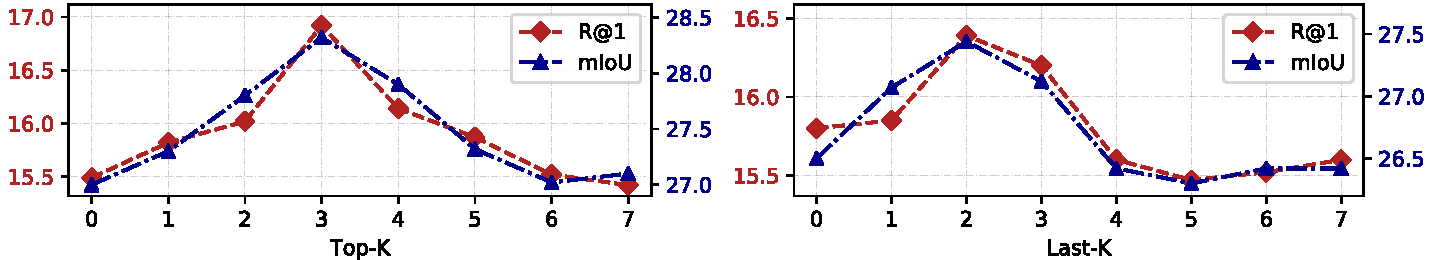
\includegraphics[width=.95\textwidth]{images/wsra_lask_K.pdf}
\centering
\caption{\small  Effect of different $K$ in the top/last-$K$ sampling on DiDeMo validation split.}
\label{figure:k_sample}
\end{figure}


% table 3
{\setlength{\tabcolsep}{.5em} % for the horizontal padding
\begin{table*}[t]
\begin{center}
\caption{ Language grounding results on the test set of Charades-STA under different intersection over unions. $^*$ denotes the work under peer reviewing.
}
\label{table:charades_sta}
\scalebox{0.75}{
\small{
\begin{tabular}{c| c | cc | cc | cc|c}
\toprule
\multirow{2}{*}{} &  \multirow{2}{*}{Approach} & \multicolumn{2}{c}{\textbf{IoU=0.3}}  & \multicolumn{2}{c}{\textbf{IoU=0.5}}  & \multicolumn{2}{c}{\textbf{IoU=0.7}}\\
 & & R@1& R@5 & R@1  & R@5   & R@1 & R@5 &  mIoU \\
\hline
\multirow{5}{*}{{\shortstack{\textit{Fully}\\Supervised}}}&Random~\citep{gao2017tall} & -- & -- & 08.51 & 37.12  & 03.03 & 14.06 & --\\
&VSA-STV \citep{kiros2015skip} & -- & --  & 10.50 & 48.43  & 04.32 & 20.21 & --\\

&CTRL~\citep{gao2017tall} & -- & -- & 21.42 & 59.11 & 07.15 & 26.91 & -- \\
&Xu \emph{et al.} ~\citep{xu2019multilevel} & -- &-- & 35.60 & 79.40  & 15.80 & 45.40 & -- \\
&MAN \citep{zhang2019man} & -- & -- & 46.53 & 86.23  & 22.72 & 53.72 & --\\

\hline 
\multirow{4}{*}{{\shortstack{\textit{Weakly}\\Supervised}}}&TGA~\citep{Mithun_2019_CVPR} & 32.14 & {89.56} & 19.94 & {65.52} & 08.84 & 33.51 & --\\
&SCN~\citep{lin2019weakly} &  42.96 & \textbf{95.56}  & 23.58 & \textbf{ 71.80}& 09.97 & {38.87} & --\\
&CTF$^{*}$~\citep{chen2020look} &  39.80 & - &  27.30 & - & \textbf{12.90} & - & --\\
% &WSRA-\textit{Verb}  & 46.50 & 73.84 & 29.35 & 60.48  & 10.05 & 33.73 & 29.05 \\
% &WSRA-\textit{Lang} & 43.63 & 73.58  & 27.02 & 55.62 & 08.87 & 26.91 & 26.68  \\
&WSRA (Ours) & \textbf{50.13} & {86.75}  & \textbf{31.20} & 70.50& {11.01} & \textbf{39.02 }& \textbf{31.00} \\
\bottomrule
\end{tabular}
}
}
\end{center}
\end{table*}
}

We compare our \textit{WSRA}  with other advanced weakly/fully-supervised methods in Table.~\ref{table:didemo}. 
As the previous methods, 
we experiment with visual features from modals of RGB and optical flow. 
Upper-bound of DiDeMo is brought since the human annotators cannot achieve 100\% agreement in 
annotating the segment boundaries \emph{w.r.t} the given video-level sentence~\citep{anne2017localizing}.
Comparing with the baseline models, 
our \textit{WSRA} model  significantly outperforms weakly supervised TGA~\citep{Mithun_2019_CVPR} by 5.5\%, 11\% at R@1 and R@5 respectively, 
even achieving comparable performance with several fully supervised methods \emph{e.g.}, CCA~\citep{anne2017localizing} and LSTM based model~\citep{anne2017localizing}. 
It is also worth noting that, our \textit{WSRA} model has similar number of parameters with all above mentioned baseline models. 
% In Fig.~\ref{figure:didemo}, we exhibit examples of the grounding attention weights together with a failure case.
% We notice that \textit{WSRA} shows high attention on the video segment that corresponds to the query. However in the second case, \textit{WSRA} fails to distinguish the video segments as the attention weights show similar values. This can be partly ascribed to the extremely alike visual contents of the video, which prevents the model from associating the descriptions with a distinct moment.



\subsubsection{Language Grounding on Charades-STA}
We further validate our \textit{WSRA} for the language grounding task on another video dataset, 
Charades-STA~\citep{gao2017tall},
which augments the Charades dataset~\citep{actorobserver,sigurdsson2017asynchronous}  with
manual annotations in the form of 
natural language descriptions at precise start-end timestamp of each video.
Charades-STA contains 12,408/3,720 video-query pairs for training/testing. 
For annotation,
Charades-STA expands each verb to generate a textual sentence
from single caption in Charades using language templates, 
and associate the sentence with frames corresponding to this verb.
To encode the video segment,
as done by other weakly-supervised methods 
for action localization~\citep{nguyen2018weakly,paul2018w},
we use the I3D feature from a pre-trained model trained over 
the Kinetics dataset~\citep{carreira2017quo}. 
For inference, we turn to the moment selection methods~\citep{gao2017tall},
which generate multi-scale sampled moment candidates using sliding window method for retrieval with fixed length of frames. 
Moreover, 
since the  video duration varies significantly, we sampling the moment 
candidates with lengths proportioned to the video duration.
Specifically, sampled candidate clips are with $\small\{$20\%, 30\%, 40\%, 50\%$\small\}$ of the whole videos and in 80\% overlap using the sliding window manner, then the moment with highest attention weight score is selected as the final prediction. More details can be found in the supplementary.
\begin{figure*}[t]
\includegraphics[width=.98\textwidth]{images/wsra_qualitative.pdf}
\centering
\caption{\small Qualitative examples of the language grounding on Charades-STA dataset. We select the top several video moments with high attention weights as the prediction.}
\label{figure:qualitative}
\end{figure*}
% \begin{figure*}[t]
% \includegraphics[width=1.0\textwidth]{images/retrieval.pdf}
% \centering
% \caption{\small Examples of the sampled ``pseudo-positive'' videos, where exist the common activity of ``\textit{watching tv}'', and irrelevant videos in a batch that serves as negative samples for learning.}
% \label{figure:sampled}
% \end{figure*} 
We report the performance comparison with
different mean Intersection-over Union (mIoU = \{0.3, 0.5, 0.7\}) and Recall@\{1, 5\}, 
and the mIoU as a summary metric.
We list detailed comparison in Table~\ref{table:charades_sta}.
From our \textit{WSRA} and TGA~\citep{Mithun_2019_CVPR}, 
we can see the clear advantage of our referring attention:  
\textit{WSRA} significantly outperforms TGA, 
for example by 18\% at [R@1, IoU=0.3], 
and 12\% at [R@1, IoU=0.5], respectively. 
We can also see clearly from the above table that, 
\textit{WSRA} demonstrates either comparable or even better performance than 
most fully-supervised methods. 
% In right side of Fig.~\ref{figure:sampled}, we showcase examples of the sampled videos during learning, our cross-video loss enables the \textit{WSRA} to exploit the common activity exist in both videos. 
In the meanwhile, our top/last-$K$ sampling also rejects theses pseudo-positive and less informative samples in the contrastive learning. Fig.~\ref{figure:qualitative} shows the qualitative examples of grounding in Charades-STA dataset where the moment is aligned with language query even facing much longer videos. We further study the effect of cross-video loss in the supplementary.
% \begin{figure*}[t]
% \centering
% \includegraphics[width=.90\textwidth]{images/didemo.pdf}
% \caption{\small We show the attention weights of language grounding on DiDeMo with a failure example. Ground-truth moment is in red-box.}
% \label{figure:didemo}
% \end{figure*}
\subsection{Conclusion}
In this paper, we propose the weakly supervised model with the referring attention mechanism (\textit{WSRA})  for learning temporal-textual association on videos.
We introduce several novel loss terms and sampling strategies,
all of which help better learning by fully exploiting the cues from 
the weak supervision at video level.
Through extensive experiments on two benchmarks,
we show the \textit{WSRA} model outperforms the state-of-the-art weakly-supervised
methods by a notable gain,
achieving on par or even better performance than some fully-supervised methods. As an outlook for the future study, we consider that the most potential aspect our model would benefit comes from the video-language representation learning at scale~\citep{miech2019howto100m}, whereas the training is often severely accompanied by uncurated annotations: \textit{e.g.}, temporally misaligned descriptions~\citep{miech2019end}. To construct a soundly and largely pre-trained model, it is requisite to properly leverage the weak or biased annotation at comprehensive views. Our \textit{WSRA} provides us with such a perspective as the trailblazer, that investigates thoroughly how language can be fully exploited as valid supervisions even without temporal annotations.                     %   \include rather than \input for chapters
%\include{chapter3}% etc. 
                                        % Heading commands (in descending order): 
                                        % \chapter
                                        % \section
                                        % \subsection
                                        % \subsubsection
                                        % \paragraph
                                        % \subparagraph
%%%%%%%%%%%%%%%%%%%%%%%%%%%%%%%%%%%%%%%
% Back matter
%%%%%%%%%%%%%%%%%%%%%%%%%%%%%%%%%%%%%%%
\SingleSpacing                          % Back matter should be single spaced 

\edef\defaulttolerance{\the\tolerance}
\tolerance 500                         % Increase tolerance to prevent material extending into margins
\hbadness 500  

\iftoggle{useendnotes}{%                % If you're using endnotes, output them here
  \setsecnumdepth{none}                 % No section numbering in end notes
%   \printpagenotes                       
  \setsecnumdepth{all}%                 % Turn section numbering back on after printing
}{}



% \iftoggle{usebiblatex}{%                % Output the bibliography
%   \printbibliography[title=\bibheading] % Using a 'biblatex' package
% }{%                                     
%   \bibliographystyle{\natbibstyle}      % Using 'natbib'
%   \bibliography{\bibfilename}
% }



% \appendix                               % Indicate start of appendices
                                        % Appendices are considered 'mainmatter' in this
                                        %   documentclass
\tolerance \defaulttolerance            % Set tolerance back to default
\hbadness \defaulttolerance  

\addtocontents{toc}{\protect%           % Only include appendix title in table of contents
  \setcounter{tocdepth}{0}}%            %   and omit sub-headings
\renewcommand*{\chapnamefont}%          % Reset font for 'Appendix' in chapter titles
    {\normalfont\MakeTextUppercase}                                        
\makeatletter                           % Clear page after printing appendix title
  \renewcommand{\memendofchapterhook}%
  {%
    \clearpage
    \m@mindentafterchapter
    \@afterheading
  }
\makeatother

\phantomsection                         % Need '\phantomsection' to place hyperref 
                                        %   bookmark more accurately
% \addcontentsline{toc}{part}{Appendix}   %~Add "Appendix" to TOC here; comment out this 
                                        %   line if you're not including appendices

%\phantomsection                        %!This is the one part of the template that I 
%\addtocontents{toc}%                   %   could not get to work properly. After you 
%  {\protect\markboth{APPENDIX}{Page}}  %   start listing appendices in the TOC, 
                                        %   subsequent TOC pages should use "APPENDIX in 
                                        %   the header instead of "CHAPTER"; however, 
                                        %   this code will make "APPENDIX" appear on the 
                                        %   the same page that the *first* appendix 
                                        %   appears on. This problem won't affect most 
                                        %   people, but if it affects you, uncomment 
                                        %   these lines and move them below where 
                                        %   the appendices are listed. Keep moving these
                                        %   lines down and checking the output until
                                        %   the TOC headers appear correctly 
                 
                 


%\include{appendix1}                     %~Insert your appendices here; I recommend to use
%\include{appendix2}                     %   \include rather than \input for appendices. 
%\include{appendix3}% etc.               %   All heading commands are the same as above,
                                         %   e.g., \chapter, \section, etc. 

\backmatter                             % Start back matter according to documentclass
\makeatletter                           % Do not clear page after printing title for
  \renewcommand{\memendofchapterhook}%  %   biographical sketch
  {%
    \m@mindentafterchapter
    \@afterheading
  }
\makeatother
%\chapter{Biographical Sketch}           %~Biographical Sketch is optional
%\input{biography}                       %<Enter the name of the .tex file containing your
                                        %   biography or omit this line and type in
                                        %   your biography here (1 paragraph) 


\end{document}